\begin{singlespacing}
\chapter{A search for new phenomena}
\label{chapter:2ljets}
%
\begin{epigraphs}
\qitem{%
An experiment is never a failure solely because it fails to
achieve predicted results. An experiment is a failure only when it also
fails adequately to test the hypothesis in question, when the data it
produces don’t prove anything one way or another.%
}%
{Robert~M.~Pirsig,
\emph{Zen and the Art of Motorcycle Maintenance},
1974~\cite{pirsig1999zen}}
\qitem{%
But there is one feature I notice that is generally missing in cargo cult
science. \ldots\
% That is the idea that we all hope you have learned in studying science in
% school --- we never say explicitly what this is, but just hope that you catch
% on by all the examples of scientific investigation. It is interesting,
% therefore, to bring it out now and speak of it explicitly.
It's a kind of scientific integrity, a principle of scientific thought that
corresponds to a kind of utter honesty --- a kind of leaning over backwards.%
}%
{Richard~Feynman,
\emph{Cargo Cult Science},
1974~\cite{feynman1974cargo}}
\end{epigraphs}
\end{singlespacing}
\noindent
The main results of this thesis are my contributions to the recently
published \atlas\ searches ``for new phenomena in events with two leptons,
jets, and missing transverse momentum''~\cite{atlas2022searches},
particularly to its electroweak part.
For brevity, we will call this publication $\twoljets$ and its electroweak
part $\twoljets$-electroweak.

This chapter follows an unusual order.
A more ordinary ordering would first present preparations made in the search
project --- blind to data ---
followed later by the results --- unblinded.%
\footnote{%
Blinding, unblinding, and their implementation in this analysis are discussed
more thoroughly in Section~\ref{sec:2ljets_unblinding}.%
}
Instead, this chapter first reports the unblinded results and follows those
with in-depth discussions of individual elements, partially in light of those
results.
This unconventional ordering makes sense for two reasons.
First, it avoids iterating over those elements twice, once before unblinding
and again after;
this search project has many little and loosely-related pieces that I attempt
to cover locally to reduce the reader's need to jump between far-flung corners
of the chapter.
Second, many design decisions can only be explained in light of
the unblinded results, since major aspects of the search were reworked in the
nineteen months between its unblinding and eventual publication.

When first meeting an \atlas\ search paper,
there are certain plots and tables that I personally prefer to find before
delving into its details.
Specifically, these include the summary plot with all signal regions,
and the model-dependent exclusion contours with their comparisons to previous
results.
This chapter begins by presenting those major plots and tables in brief in
Section~\ref{sec:2ljets_splash}.
The meat of the chapter follows.
\begin{itemize}
\item Context from previous searches and inspirations for the design goals
of the $\twoljets$-electroweak search are described in
Section~\ref{sec:2ljets_context}.
\item Data, their event variables and the reconstructed objects from which
they derive are described in Section~\ref{sec:2ljets_events}.
\item Region designs for the $\twoljets$-electroweak search are described and
explained in Section~\ref{sec:2ljets_design}.
\item The modelling of our uncertain predictions of background and signal
contributions in those regions is covered in
Section~\ref{sec:2ljets_modelling}.
\item Some validation studies are presented in
Section~\ref{sec:2ljets_validation}.
\item The unblinding procedure of this search is discussed in
Section~\ref{sec:2ljets_unblinding},
\item Some additional details of our results are presented in
Section~\ref{sec:2ljets_results}.
\item A concluding discussion is given in
Section~\ref{sec:2ljets_discussion}.
\end{itemize}


\subsection{Splash summary}
\label{sec:2ljets_splash}
% begin with physics content and results
The summary plot in Figure~\ref{fig:2ljets_summary} displays unblinded results
in all main regions of the $\twoljets$-electroweak analysis.
Since this figure appears to represent the data and background estimates,
on which all derived results depend, it could be seen as the keystone of this
thesis.
There are, however, caveats to be developed later in this chapter ---
the backgrounds plotted are not exactly estimates, but are adapted and fitted
to the observed data.
In numerous orthogonal signal regions, no significant excess is observed
above the displayed post-fit backgrounds.
Indeed, there are some significant deficits of data are below the assigned
backgrounds.

% summary plot
\begin{figure}[tp]
\centering
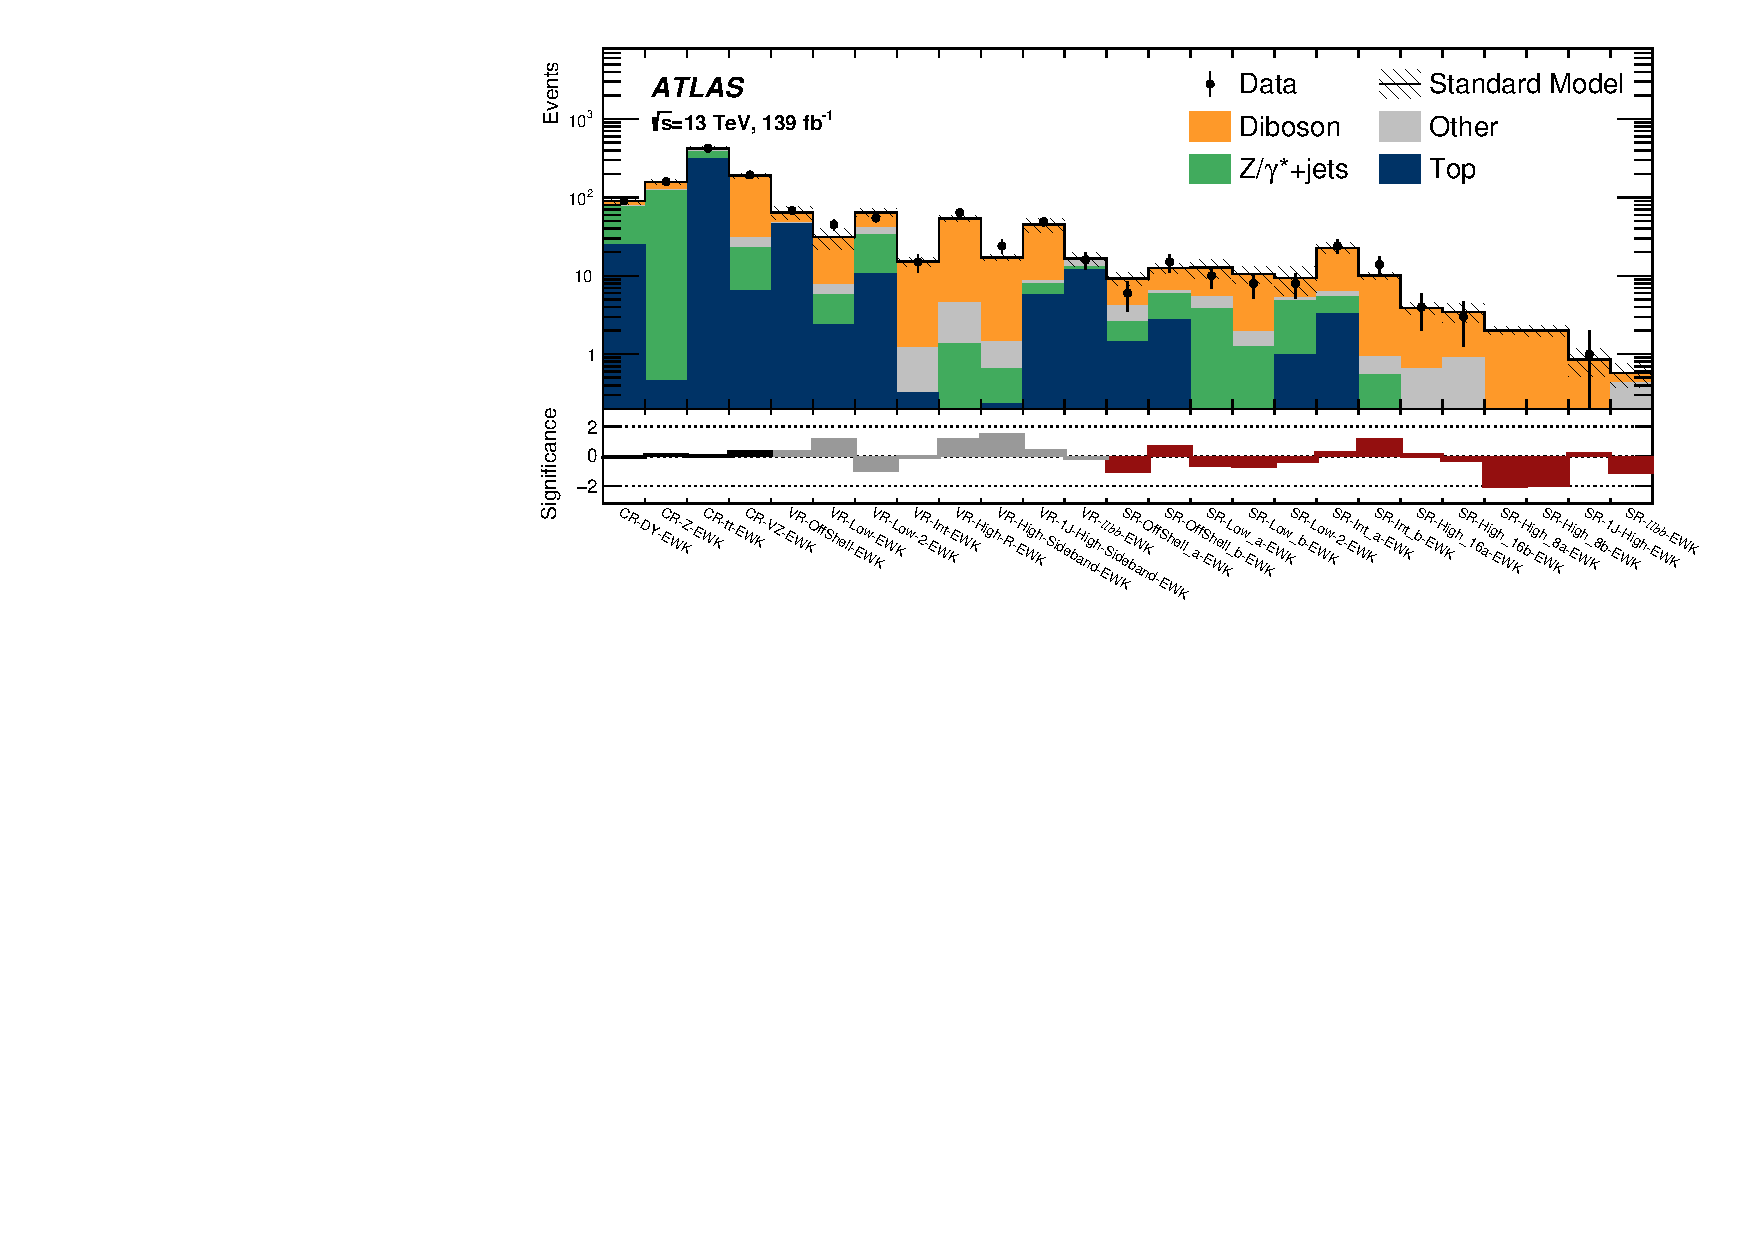
\includegraphics[width=\textwidth]{figures/2ljets_summary_log.pdf}
\caption[
Data of the $\twoljets$-electroweak analysis with \emph{post-fit}
backgrounds
]{%
Data of the $\twoljets$-electroweak analysis with \emph{post-fit}
backgrounds~\cite{atlas2022searches}.
The lower panel shows the \atlas-recommended significance
measure~\cite{atlas_significance}.
Control, validation and signal regions are shown from left to right, with the
regions within each category ordered approximately by their typical
missing transverse momentum ($\met$).
Validation region likelihoods do not directly constrain the fit.
The ``Top'' category contains $\ttbar$ and $tW$ processes, and
``Other'' contains fake/non-prompt lepton, Higgs, triboson, $\ttbar Z$, and
\topother\ processes.%
}
\label{fig:2ljets_summary}
\end{figure}

To test non-standard (supersymmetric) models against observation,
we add signal yields on top of the modelled backgrounds.

The $\twoljets$-electroweak search uses two signal models,
which we name C1N1 and GMSB and illustrate with diagrams in
Figure~\ref{fig:2ljets_signal_diagrams}.
One is an MSSM chargino-neutralino model (C1N2) that acts to produce
$\chargino_1\textrm{--}\neutralino_2$ pairs (via off-shell $W^\pm$ resonances),
that decay via $W\to q\bar q$ and $Z\to \ell^\pm \ell^\mp$
respectively to produce two leptons, jets, and two $\neutralino_1$ LSPs.
The other is a GMSB model which, from a variety of initial states, produces
$\neutralino_1\textrm{--}\neutralino_1$ pairs that decay via Higgs and $Z$
bosons, with variable branching fractions,
to final states again containing $\ell^\pm \ell^\mp$, hadronic partons,
and invisible gravitinos.
Example effects of these signal models are displayed in signal regions of the
$\twoljets$-electroweak search in
Figure~\ref{fig:2ljets_signal_examples}.
All of these regions require two leptons, jets, and
missing transverse momentum, and the signal expectations would be added on top
of the backgrounds if nature realized these supersymmetric models.

% signal diagrams
\begin{figure}[tp]
\centering
\begin{subfigure}{0.48\textwidth}
\centering
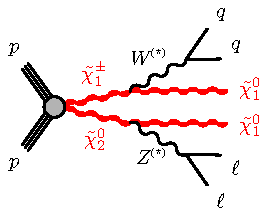
\includegraphics[width=\textwidth]{figures/2ljets_c1n2_llqqn1n1_wz.pdf}
\caption{C1N2}
\end{subfigure}
\hfill
\begin{subfigure}{0.48\textwidth}
\centering
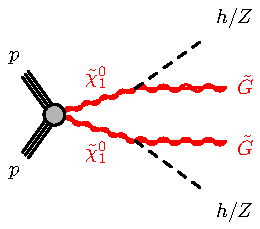
\includegraphics[width=\textwidth]{figures/2ljets_n1n1_hhggzz.pdf}
\caption{GMSB}
\end{subfigure}
\caption[
Supersymmetric signal processes in the $\twoljets$-electroweak analysis
]{%
Supersymmetric signal processes in the $\twoljets$-electroweak analysis.
\emph{Figures are reproduced from the paper%
}~\cite{atlas2022searches, atlas_susy_feynman}.
\\[0.4em]
(a) C1N2, where the initial $\chargino_1\textrm{--}\neutralino_2$ pair
is produced through an $s$-channel $W^{\pm}$ resonance and the masses of
weak bosons in decays are bounded by the mass splitting
$m(\chargino_1, \neutralino_2) - m(\neutralino_1)$.
We explore the parameters
$m(\chargino_1, \neutralino_2)$ and $m(\neutralino_1)$.
\\[0.4em]
(b) GMSB, where the initial $\neutralino_1\textrm{--}\neutralino_1$ pair
is produced by soft decays from pairs including $\chargino_1$,
$\neutralino_2$ or $\neutralino_1$.
Although the Higgs and $Z$ bosons can decay to many states, we target events
with $Z\to \ell\ell$ and $h/Z\to bb/jj$.
We explore the parameters
$m(\neutralino_1)$ and $B(\neutralino_1 \to h \tilde{G})$ with a tiny
fixed mass splitting of
$m(\chargino_1, \neutralino_2) - m(\neutralino_1) = 1\,\eV[G]$.%
}
\label{fig:2ljets_signal_diagrams}
\end{figure}

% signal region plots
\begin{figure}[tp]
\centering
\begin{subfigure}{0.495\textwidth}
\centering
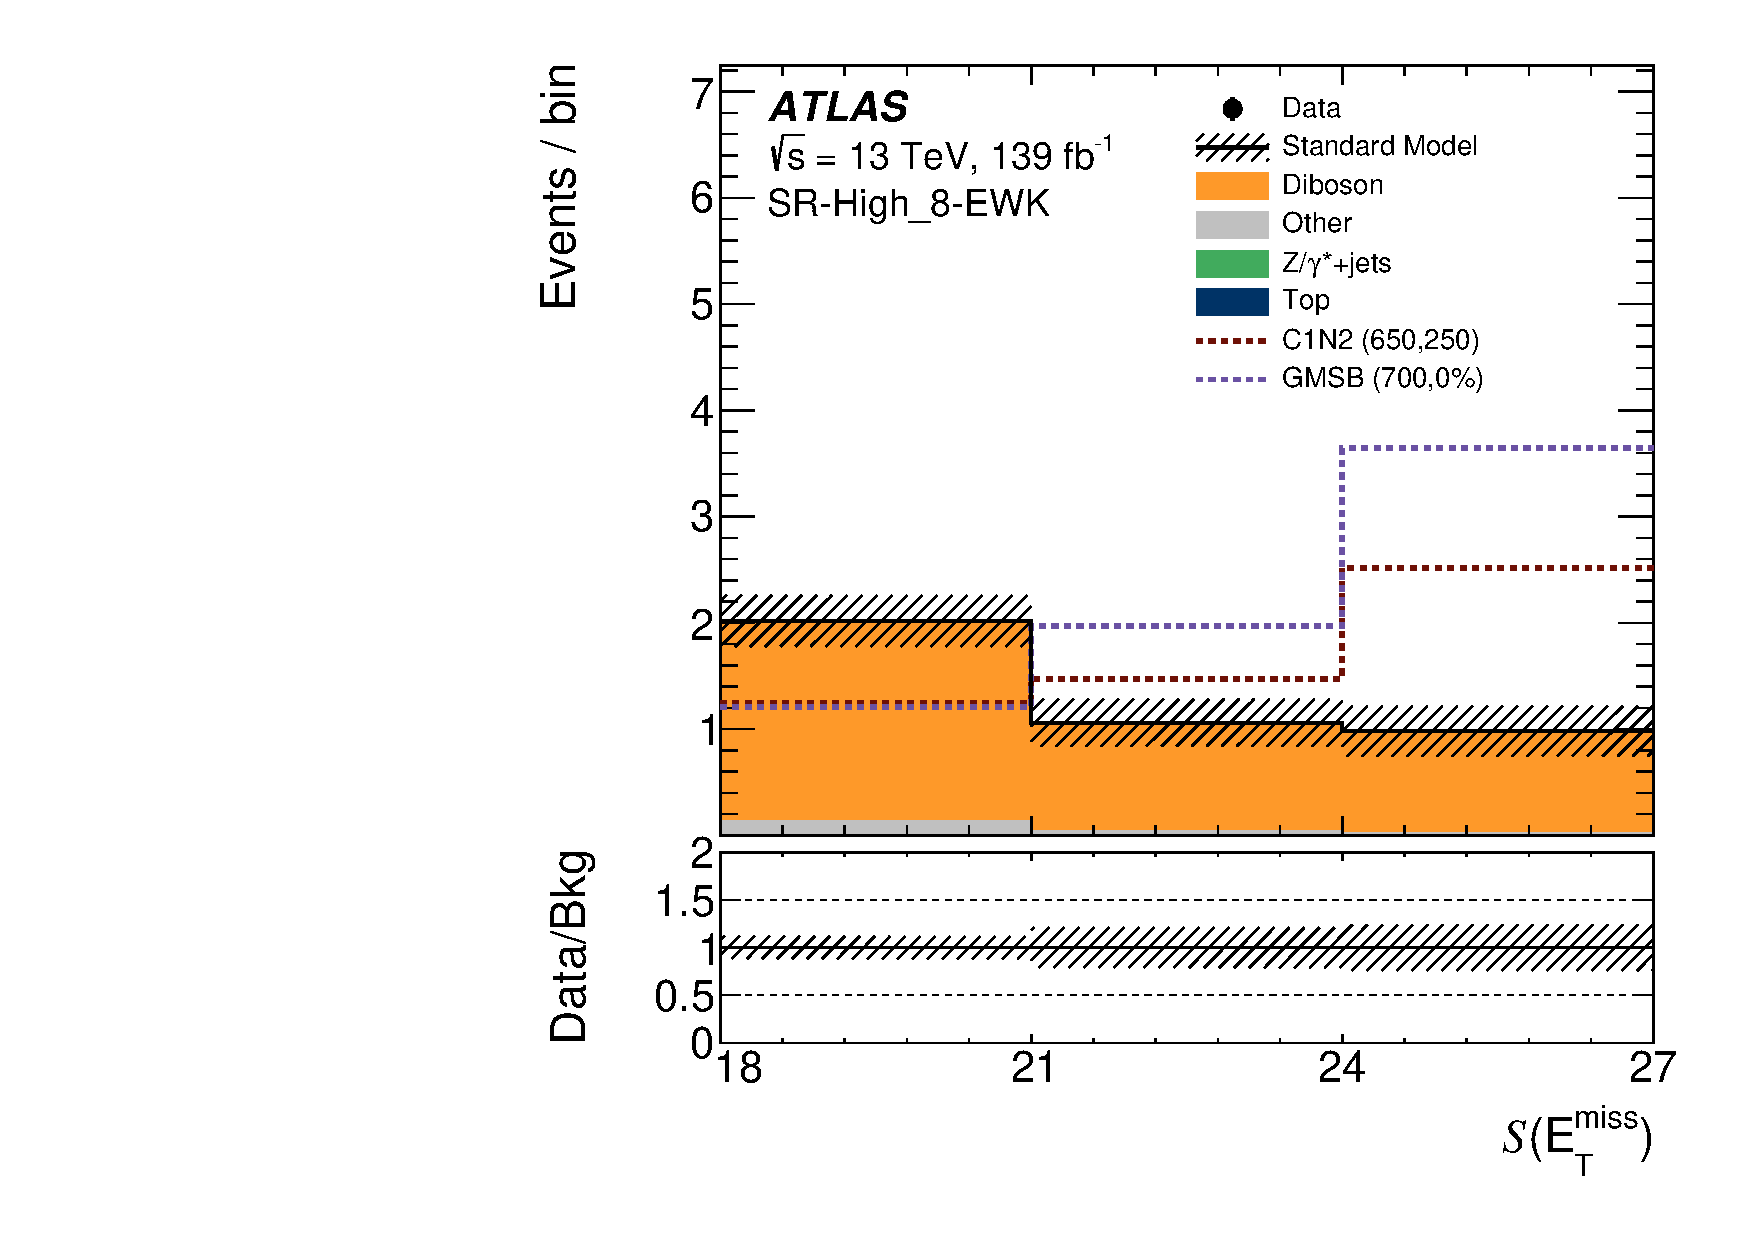
\includegraphics[width=\textwidth]{figures/2ljets_sr_high_8_met_sig.pdf}
\caption{SR-High-8}
\end{subfigure}
\hfill
\begin{subfigure}{0.495\textwidth}
\centering
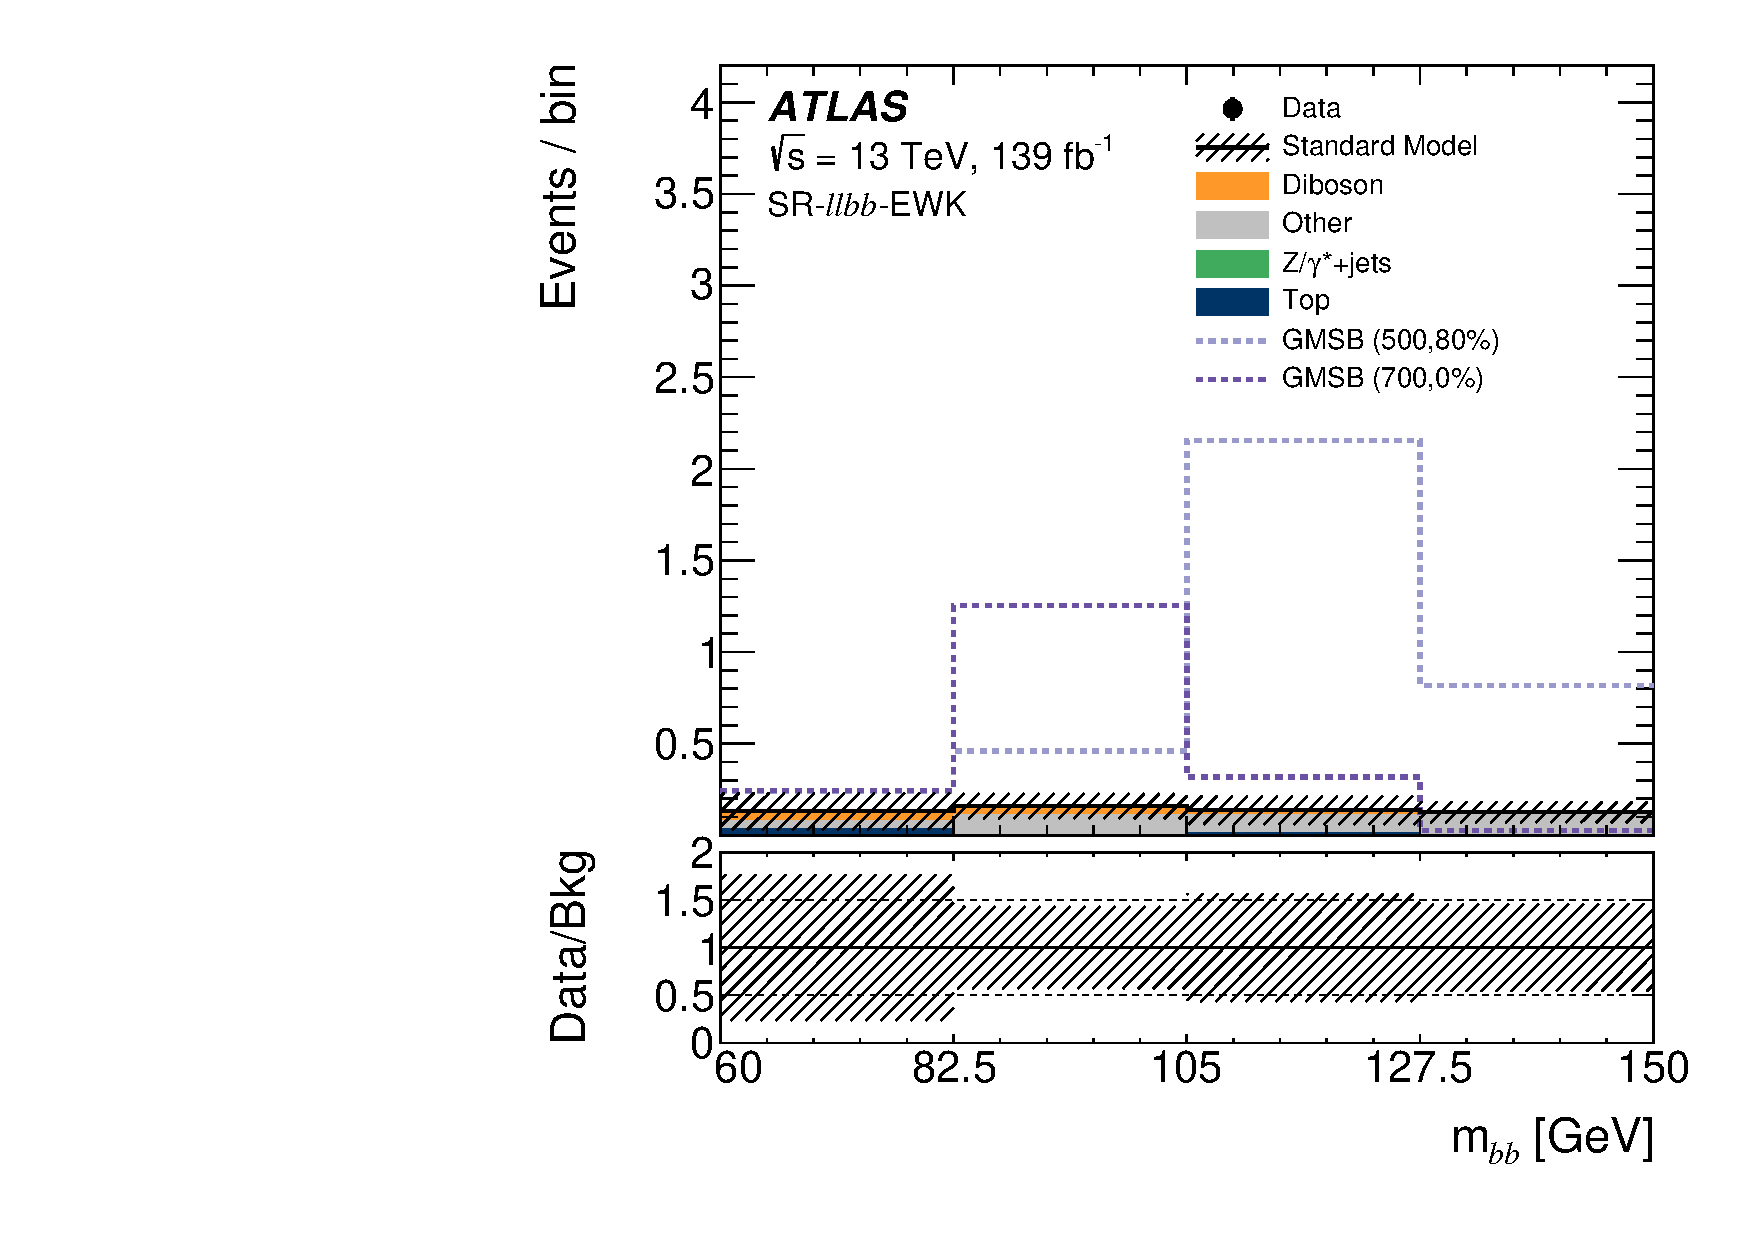
\includegraphics[width=\textwidth]{figures/2ljets_sr_llbb_mbb.pdf}
\caption{\srllbb}
\end{subfigure}
\\[0.4em]
\begin{subfigure}{0.495\textwidth}
\centering
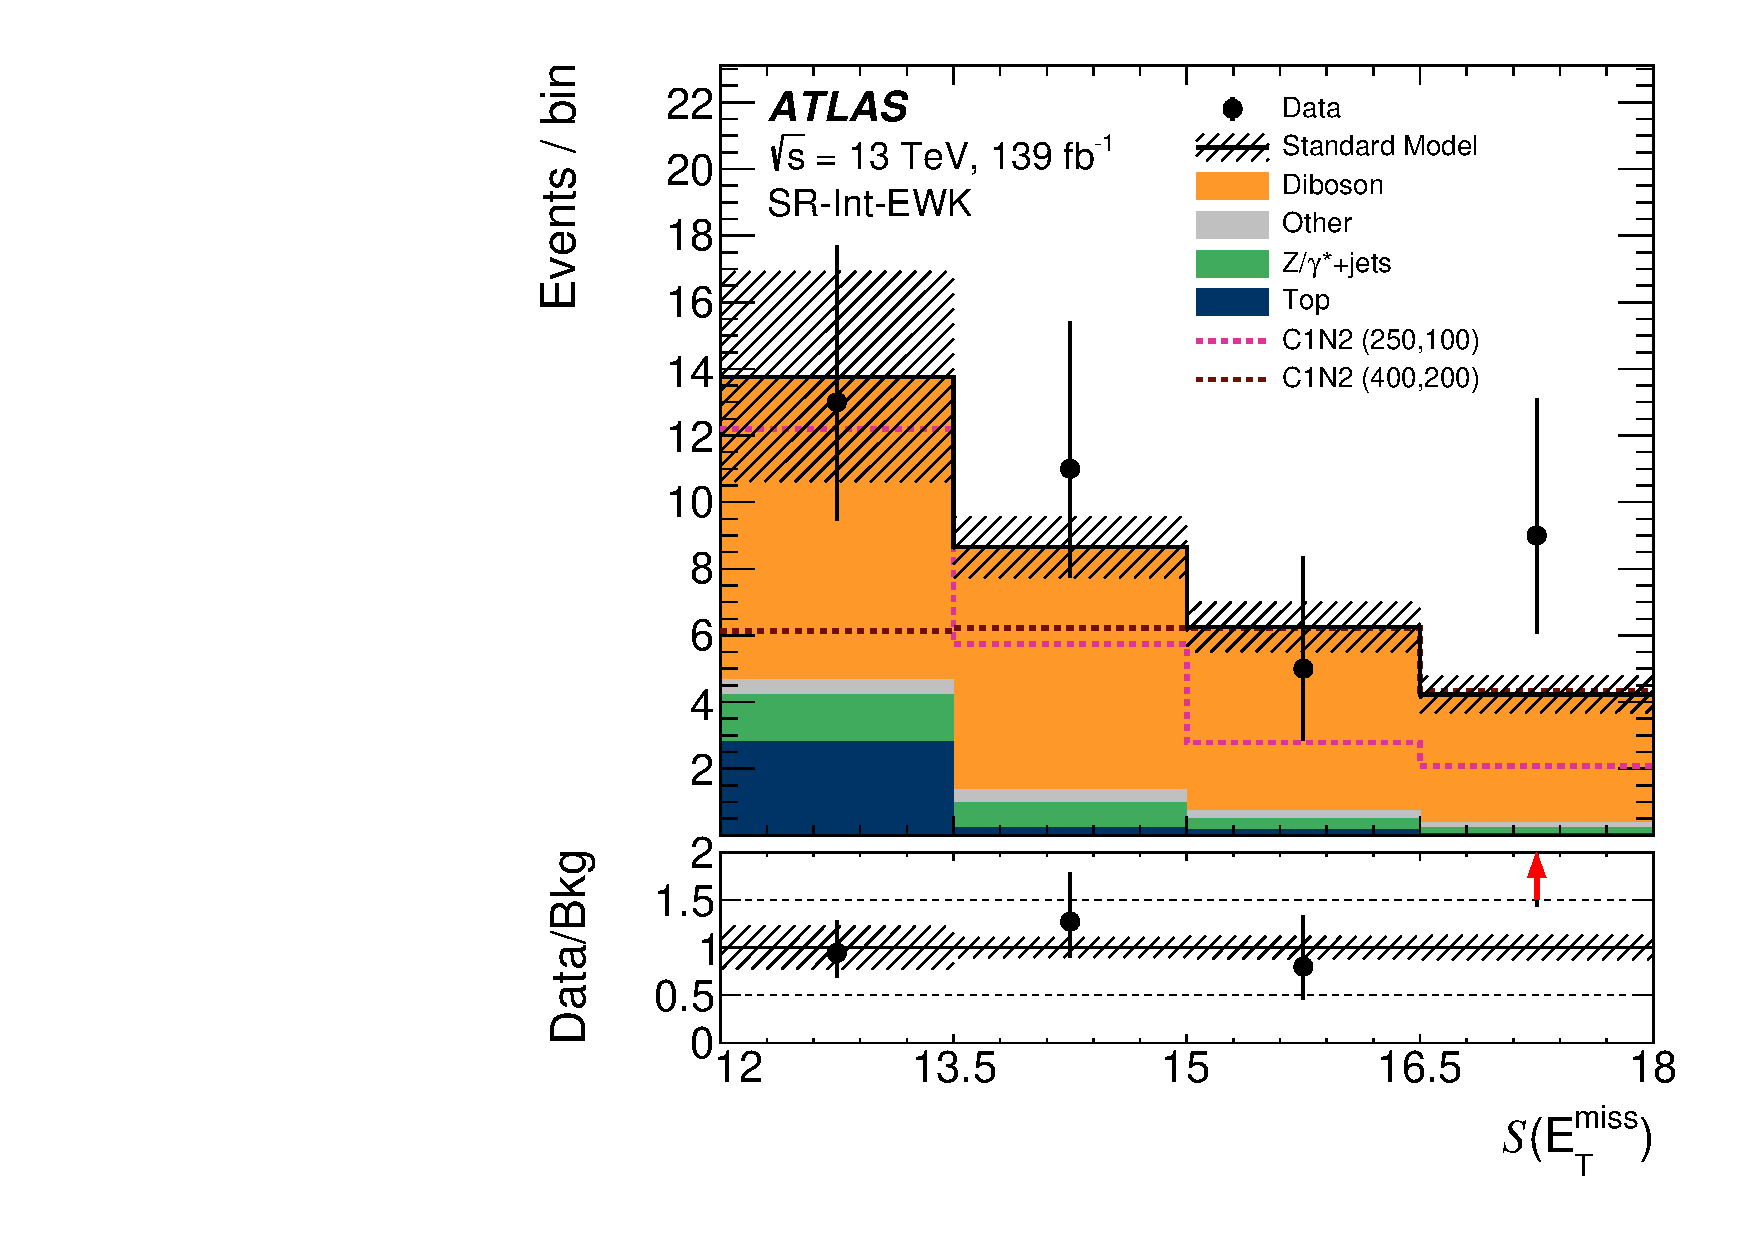
\includegraphics[width=\textwidth]{figures/2ljets_sr_int_met_sig.pdf}
\caption{SR-Int}
\end{subfigure}
\hfill
\begin{subfigure}{0.495\textwidth}
\centering
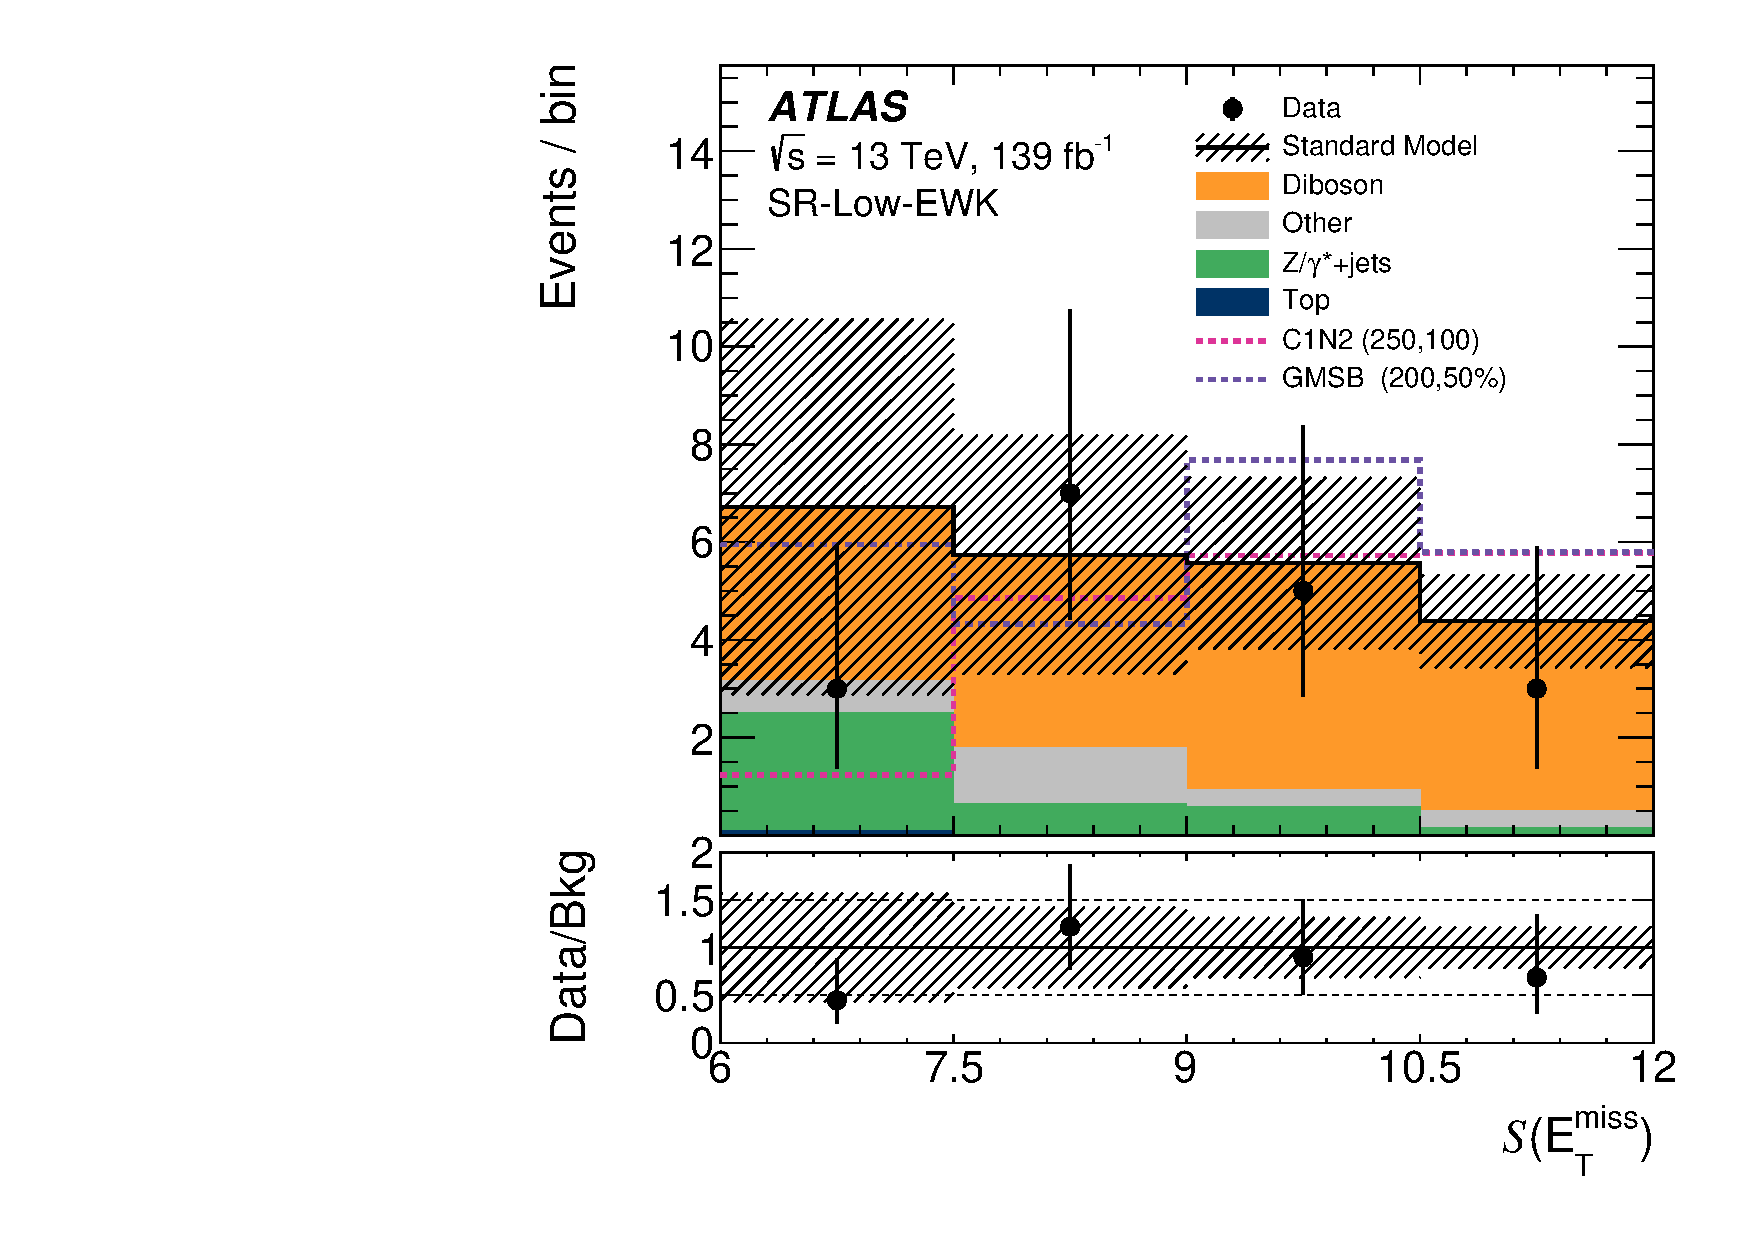
\includegraphics[width=\textwidth]{figures/2ljets_sr_low_met_sig.pdf}
\caption{SR-Low}
\end{subfigure}
\caption[
Example signal region histograms with benchmark signal sample yields overlaid
]{%
Example signal region histograms with benchmark signal sample yields overlaid
as dotted lines~\cite{atlas2022searches}.
Physically, signal yields would add on top of the backgrounds.
Unblinded data are shown --- regions in the top two plots observe zero data
and the error bars for zero events are hidden for aesthetic reasons.
\\[0.4em]
The event variable $\metsig$ is the missing transverse momentum significance,
defined in Section~\ref{sec:2ljets_metsig}, and $\mbb$ is the invariant mass of
the vector sum of the hardest two $b$-tagged jets.
}
\label{fig:2ljets_signal_examples}
\end{figure}

Both signal models have two free parameters that our search varies.
At each parameter point of a signal model, the search proceed by evaluating
event rates (yields) from that signal model with those parameters,
and considering what would happen if those event yields were added to a
Standard Model background.
Each signal-plus-background model is then tested against observed data in the
$\cls$ prescription.
From these tests, contours showing which parameters of those signal models are
labelled as excluded are derived, and displayed in
Figure~\ref{fig:2ljets_contours_c1n2} for C1N2 and in
Figure~\ref{fig:2ljets_contours_gmsb} for GMSB.
In both of these figures, space to the lower left of the contours is
labelled as excluded, and space on the other side of the observed limit contour
is not excluded.
The observed contours are somewhat larger than expected due to observed
deficits in data that we have shown in Figure~\ref{fig:2ljets_summary}.

% exclusion plots
\begin{figure}[tp]
\centering
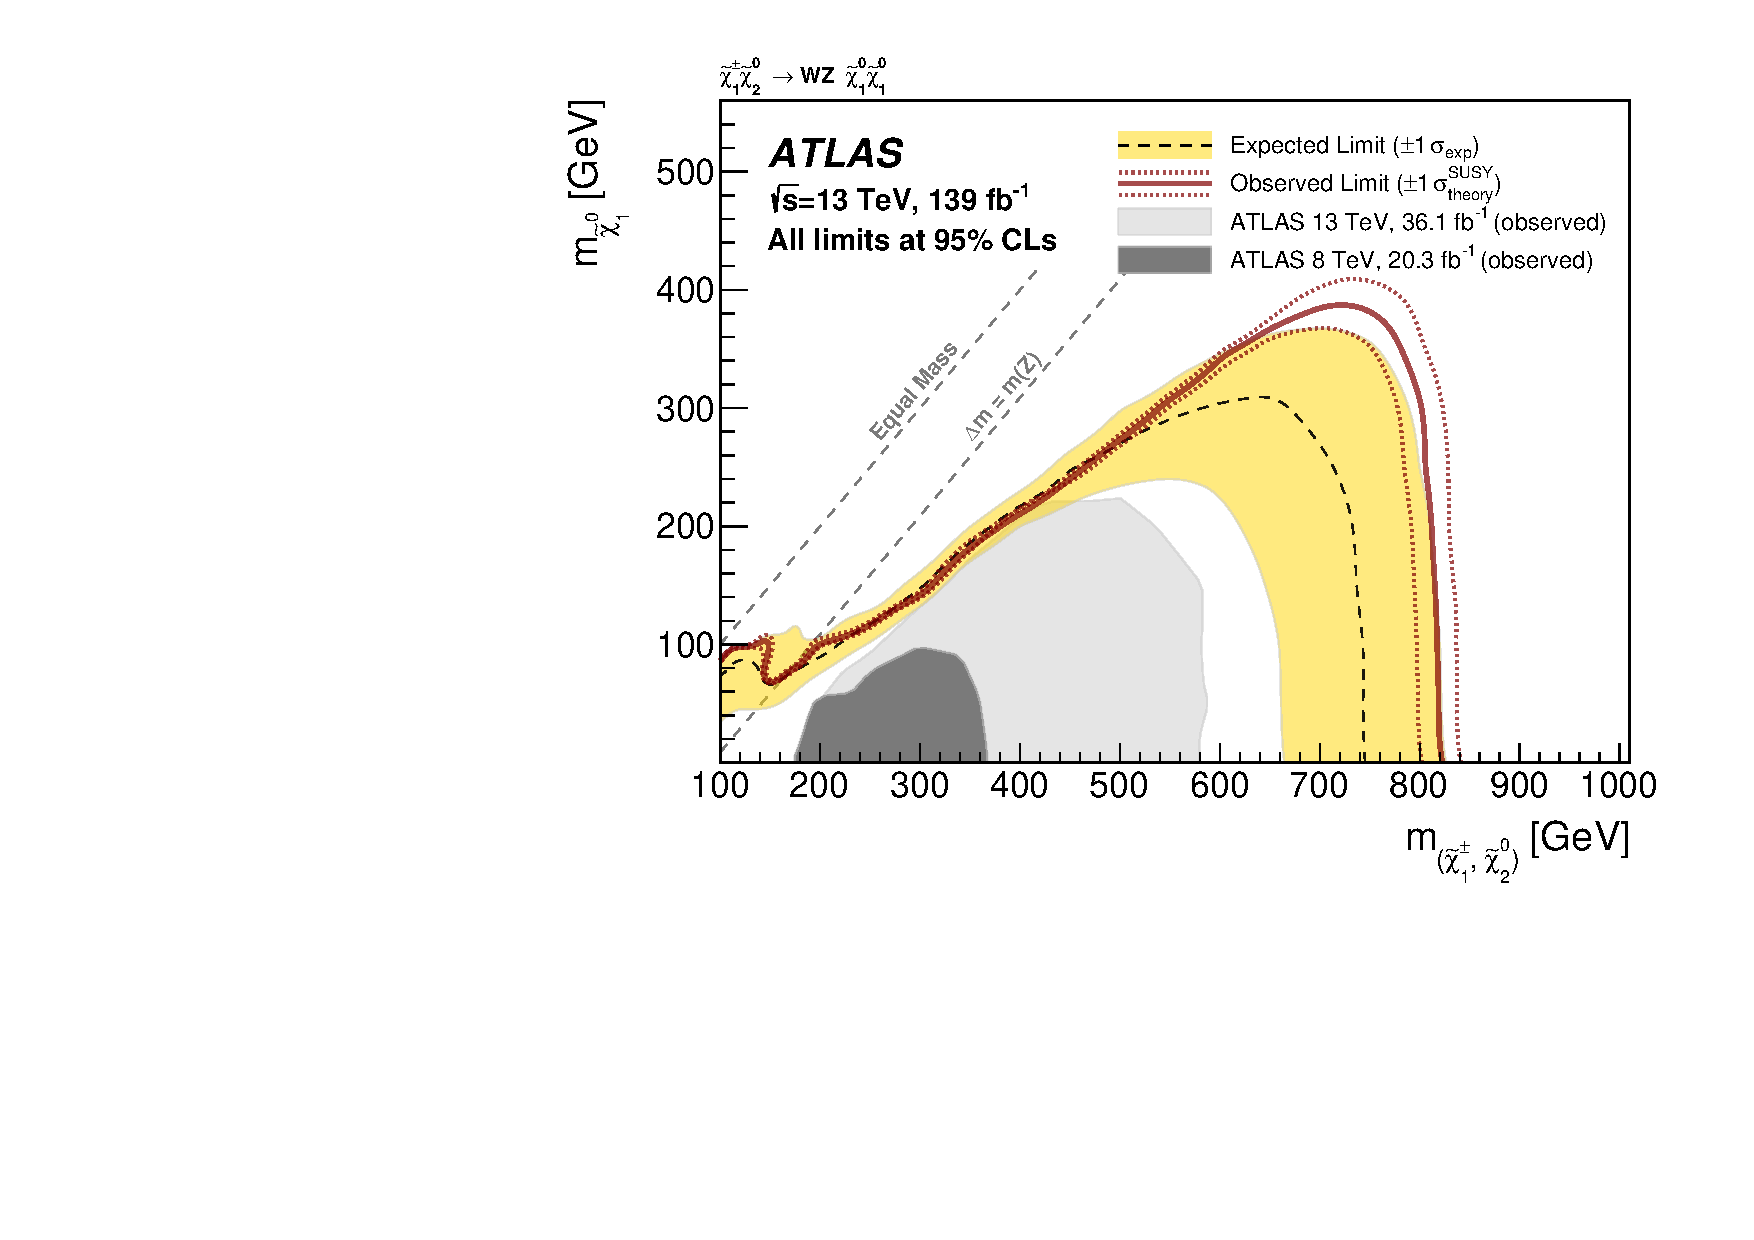
\includegraphics[width=0.99\textwidth]{figures/2ljets_contours_c1n2.pdf}
\caption[
Contours for the C1N2 model in the $\twoljets$-electroweak search
]{%
Contours for the C1N2 model in the $\twoljets$-electroweak
search~\cite{atlas2022searches}.
\\[0.4em]
Space below the solid red line is labelled as excluded, and its dotted
neighbours show alternative results that are obtained if all signal
cross-sections are varied up and down by factors intended to describe the size
of the theoretical uncertainties.
\\[0.4em]
The yellow band shows the $\pm1$-sigma region of exclusion contours
from asymptotic approximations to the distribution of the test statistics.
Grey areas are observed limits from the two-lepton results from previous
\atlas\ searches~\cite{atlas_23l_SUSY_2016_24, atlas_2l_SUSY_2013_11}.
Exclusion is defined by the $95\%$ $\cls$ prescription
with asymptotic approximations~\cite{Cowan:2010js}.
All contours are interpolated from a sparse grid.
The mass splitting is notated by
$\Delta m = m(\chargino_1, \neutralino_2) - m(\neutralino_1)$.
\\[0.4em]
This simplified model assumes that
$m(\chargino_1) = m(\neutralino_2) = m(\chargino_1, \neutralino_2)$.
}
\label{fig:2ljets_contours_c1n2}
\end{figure}

\begin{figure}[tp]
\centering
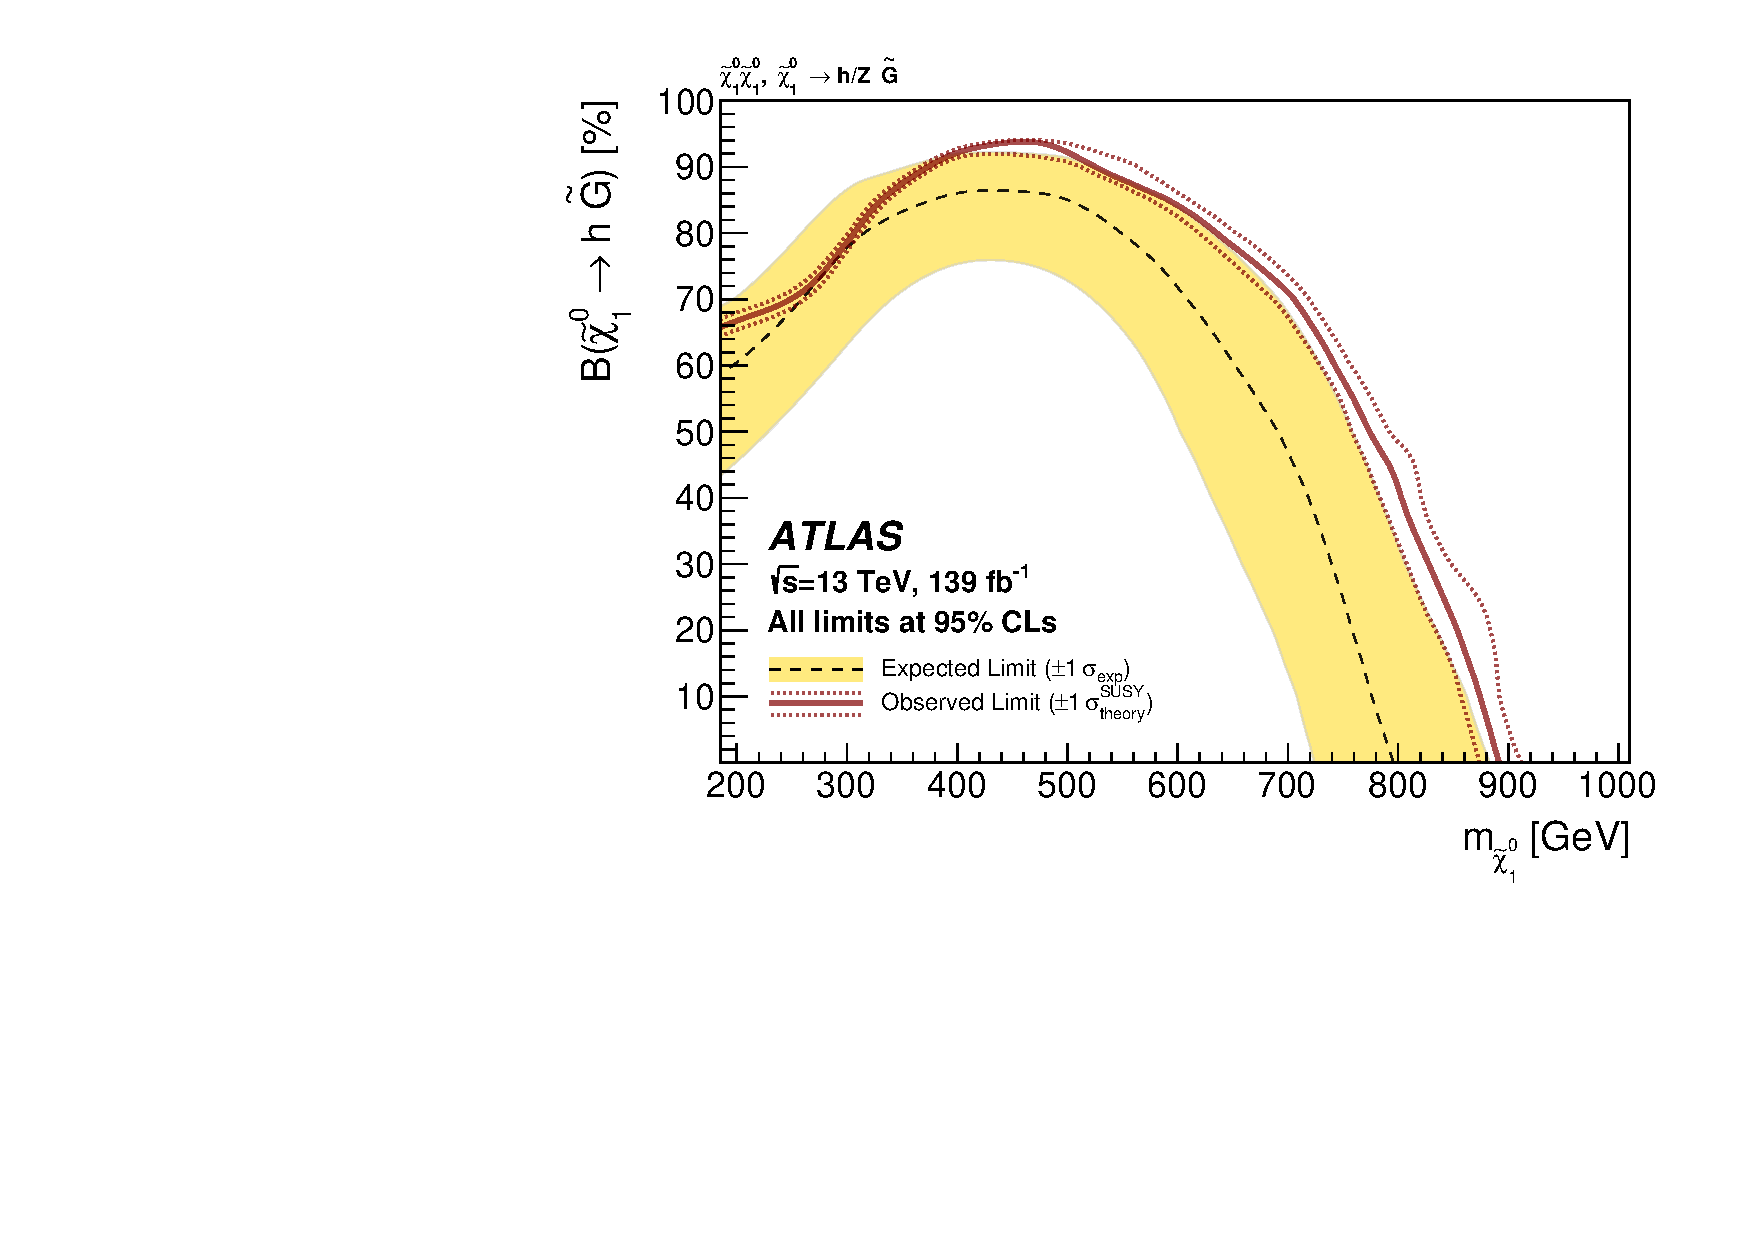
\includegraphics[width=0.99\textwidth]{figures/2ljets_contours_gmsb.pdf}
\caption[
Contours for the GMSB model in the $\twoljets$-electroweak search
]{%
Contours for the GMSB model in the $\twoljets$-electroweak
search~\cite{atlas2022searches}.
\\[0.4em]
Space below the solid red line is labelled as excluded, and its dotted
neighbours show alternative results that are obtained if all signal
cross-sections are varied up and down by factors intended to describe the size
of the theoretical uncertainties.
\\[0.4em]
The yellow band shows the $\pm1$-sigma region of exclusion contours
from asymptotic approximations to the distribution of the test statistics.
No previous limits have been set on this model by two-lepton
\atlas\ searches~\cite{atlas_23l_SUSY_2016_24, atlas_2l_SUSY_2013_11}.
Exclusion is defined by the $95\%$ $\cls$ prescription
with asymptotic approximations~\cite{Cowan:2010js}.
All contours are interpolated from a sparse grid.
}
\label{fig:2ljets_contours_gmsb}
\end{figure}

Signal regions of the $\twoljets$-electroweak analysis are combined to form
five discovery regions.
Results of their model-independent interpretations are presented in
Table~\ref{tab:2ljets_discovery}.
The same data deficits drive stronger bounds on possible signals that manifest
as smaller limits on the signal expectations, which are labelled
$S_{\mathrm{obs}}^{95}$ in the figure.
\footnotetext{%
The visible cross-section is defined such that the expected event count is
given by the product of $A\epsilon\sigma\times L$, where $L$ is the integrated
luminosity (typically in $\mathrm{fb}^{-1}$ units).
This particular presentation is uses an `acceptance' $A$, an
`efficiency' $\epsilon$, and an observable cross-section $\sigma_{\mathrm{obs}}$
(presented here at at $95\%$ limit).
The acceptance and efficiency are defined using truth-level simulations, in
which the $A$ is the fraction of truth-level events that pass selection
requirements, and $\epsilon$ is the ratio from the truth-level yield to the
reconstruction-level yield.
Because detector effects can increase yields, this $\epsilon$ can exceed
one~\cite{susy_results_presentation_papers}.
}

% upper limits
\begin{table}[tp]
\centering
% custom separator for aligned +-
% https://stackoverflow.com/a/2132998
\begin{tabular*}{\textwidth}{l|r@{$~\pm~$}lcccccc}
& \multicolumn{2}{c}{Fitted}
& Data
& $A\epsilon\sigma_{\mathrm{obs}}^{95}\,\mathrm{fb}$
& $S_{\mathrm{obs}}^{95}$
& $S_{\mathrm{exp}}^{95}$
& $\clb$
& $p_{s\!=\!0}$
\\
\hline
DR-OffShell & $22.1$ & $2.7$ & $21$ & $0.10$ & $14.3$ & $12.3^{+4.7}_{-3.1}$ & $0.68$ & $0.50$
\\[.5ex]
DR-Low & $22$ & $4$ & $18$ & $0.08$ & $10.8$ & $15.3^{+5.7}_{-4.0}$ & $0.09$ & $0.50$
\\[.5ex]
DR-Int & $35$ & $4$ & $38$ & $0.15$ & $20.9$ & $17.5^{+5.9}_{-3.9}$ & $0.73$ & $0.23$
\\[.5ex]
DR-High & $3.9$ & $0.5$ & $0$ & $0.02$ & $3.0$ & $5.6^{+2.2}_{-1.5}$ & $0$ & $0.50$
\\[.5ex]
DR-$\llbb$ & $0.51$ & $0.20$ & $0$ & $0.02$ & $3.0$ & $3.0^{+1.3}_{-0.0}$ & $0.19$ & $0.50$
\\[.5ex]
\end{tabular*}
\caption[
Upper limit results in $\twoljets$-electroweak discovery regions
]{%
Upper limit results in $\twoljets$-electroweak discovery
regions~\cite{atlas2022searches}.
Each fitted yield is in the background-only model constrained by the data in
all control regions and the discovery region.
Limits are intended to reflect constrains on additive signal contributions.
\\[0.4em]
Left to right:
the region name,
the post-fit background expectation,
the number of data observed,
the observed $95\%$ $\cls$ upper limit on the visible cross-section
(labelled $A\epsilon\sigma_{\mathrm{obs}}^{95}\,\mathrm{fb}$\footnotemark),
its corresponding signal expectation $S_\mathrm{obs}^{95}$,
the expected $95\%$ upper limits on the signal expectation $S_\mathrm{exp}^{95}$
as would be obtained were the test statistic given by its central or
$\pm1$-sigma variations,
$\clb$ (as defined in Section~\ref{sec:searches_cls}) evaluated with the signal
expectation set to the observed upper limit,
and the discovery $p$-value capped at $0.5$.
The cross-section and signal yield limits are related by a factor of our
integrated luminosity $139.0\,\mathrm{fb}^{-1}$.
\\[0.4em]
Upper limits use the one-sided profile likelihood test
statistic~\cite{Cowan:2010js}.
The discovery $p$-value uses a profile likelihood test statistic in a one-sided
test.
All $p$-values are estimated by ``toy'' simulations of alternative data.
Values with errors are rounded according to the PDG rounding
scheme~\cite{pdg2022ynf}.%
}
\label{tab:2ljets_discovery}
\end{table}


\subsection{Contributions}
Many people contributed directly and indirectly to the $\twoljets$ searches.
I claim personal responsibility for the following parts of the $\twoljets$
search and related \atlas\ efforts.
\begin{itemize}
\item Design, implementation, and execution of the electroweak part of the
analysis.
\item Service as Analysis Contact (a management role) for the $\twoljets$
project from January to October 2020.
\item Production of main data inputs for all three $\twoljets$ searches
and the Recursive Jigsaw Reconstruction (RJR) $3\ell$
search~\cite{atlas_rjr_3l_SUSY_2019_09}.
Production of all experimental systematic variations for the background
samples --- other group members assisted with the central background sample.
Production of all electroweak signal samples and their systematic variations.
\item Evaluation of $Z$+jets uncertainties for RJR signal regions from
simulations. Their variations exceeded $100\%$ relative variation and supported
the use of data-driven methods.
\item Various collaborations with all other group members on common core tasks
that are shared between the searches of the $\twoljets$ project.
\item Integration of the electroweak analysis with \atlas\ combinations and
pMSSM scan efforts, by performing their validation studies and serializing the
analysis results.
\item Preparation of electroweak results for publication in the
paper~\cite{atlas2022searches} and the public HEPData
archive~\cite{maguire2017hepdata}.
\end{itemize}
Except where specified, I produced all figures presented in this thesis.
Many plotting scripts, however, are modified from versions inherited from
many past and present \atlas\ members, to whom I am grateful.

Of the large collaboration involved in this project, a great deal of credit is
due to the following colleagues, labelled with their primary focus within
the $\twoljets$ search effort:
Knut~Oddvar Vadla (electroweak, core),
Sarah~Williams (electroweak),
Jason~Oliver (RJR),
Abhishek~Sharma (RJR),
Jonathan~Long (strong),
Arka~Santra (strong, RECAST),
Matt~Zhang (strong),
Yumeng~Cao (electroweak, strong),
Eirik~Gramstad (fake/non-prompt leptons),
Benjamin~Hooberman (leadership).
Cheers.


\section{Summaries}
\label{sec:2ljets_context}
% previous results on 2(/3)L from ATLAS
% other constraints on these models from ATLAS/CMS
% previous region design, motivation for this work
Previous analyses of \atlas\ data have explored similar selections of
two leptons, jets, and missing transverse momentum.
Quite a few analyses, in fact ---
this search project exists to supplement those results with information from
the full LHC Run~2 data-set that was collected in the years $2015$
through to $2018$ and contains
$139~\mathrm{fb}^{-1}$ of usable proton-proton collisions at
$\sqrt{s} = 13\,\eV[T]$.
Leveraging the increased data quantity is one key contribution of $\twoljets$.
How well those data are used depends on how well the search is designed, so
$\twoljets$ further benefits from lessons learned from the experiences of
past analyses.

The $\twoljets$ analysis is a trinity in which all three parts update
previously published \atlas\ results.
These three parts are named `RJR', `electroweak', and `strong',
and this section describes each in its historical context.

Recursive Jigsaw Reconstruction (RJR) is an algorithm for constructing useful
event variables that target given decay trees.
The $\twoljets$-RJR analysis, detailed in Section~\ref{sec:2ljets_origins_rjr},
uses RJR variables to define its regions in a signal-independent search.

The $\twoljets$-strong analysis is
detailed in Section~\ref{sec:2ljets_origins_strong} and
searches for effects from supersymmetric models that are active in the strong
sector.
It uses conventional (non-RJR) event variables and focuses on features in the
distribution of the invariant masses of lepton pairs.
That dilepton mass distribution can have distinct features that would stand
out from Standard Model backgrounds and depend on the masses of decaying
supersymmetric resonances.

My primary contributions are to the $\twoljets$-electroweak search,
detailed in Section~\ref{sec:2ljets_origins_electroweak}, that seeks effects
from supersymmetric models that are active in the electroweak
sector by using conventional event variables to define a collection of
orthogonal selection regions.


\subsection{RJR}
\label{sec:2ljets_origins_rjr}
The Recursive Jigsaw Reconstruction (RJR) method interprets reconstructed
particle data by reconciling them with user-specified decay trees, and operates
by making decisions of how to assign four-momenta to different `systems',
which are represented as nodes on the chosen decay graph.
Various RJR event variables are then defined in those systems' rest
frames~\cite{jackson2017sparticles, jackson2017rjr}.

In this way, RJR variables have some intelligence in how parent particles are
reconstructed from their visible decay products, as well as approximate
independence from uninteresting boosts, particularly those from the emission of
QCD jets outside the main supersymmetric decay tree.

Over the last several years, RJR event variables have been demonstrated to be
effective for interpreting supersymmetric particle physics
data~\cite{santoni2018probing},
and have been used in numerous \atlas\ searches~\cite{
atlas_rjr_SUSY_2016_07,
atlas_rjr_SUSY_2016_15,
atlas_rjr_SUSY_2016_16,
atlas_rjr_23l_SUSY_2017_03,
atlas_rjr_SUSY_2018_12,
atlas_rjr_EXOT_2019_19,
atlas_rjr_3l_SUSY_2019_09
}.
They have also influenced the designs of other analyses that do not themselves
use RJR variables~\cite{atlas_rjr_mimic_SUSY_2018_06}.

Two decay trees are used in the $\twoljets$-RJR analysis, and from each
one signal region is defined and explored.
These trees are illustrated in Figure~\ref{fig:2ljets_rjr_decay_trees} and
target C1N2-like scenarios similar to those also targetted by the
$\twoljets$-electroweak search.

\begin{figure}[tp]
\centering
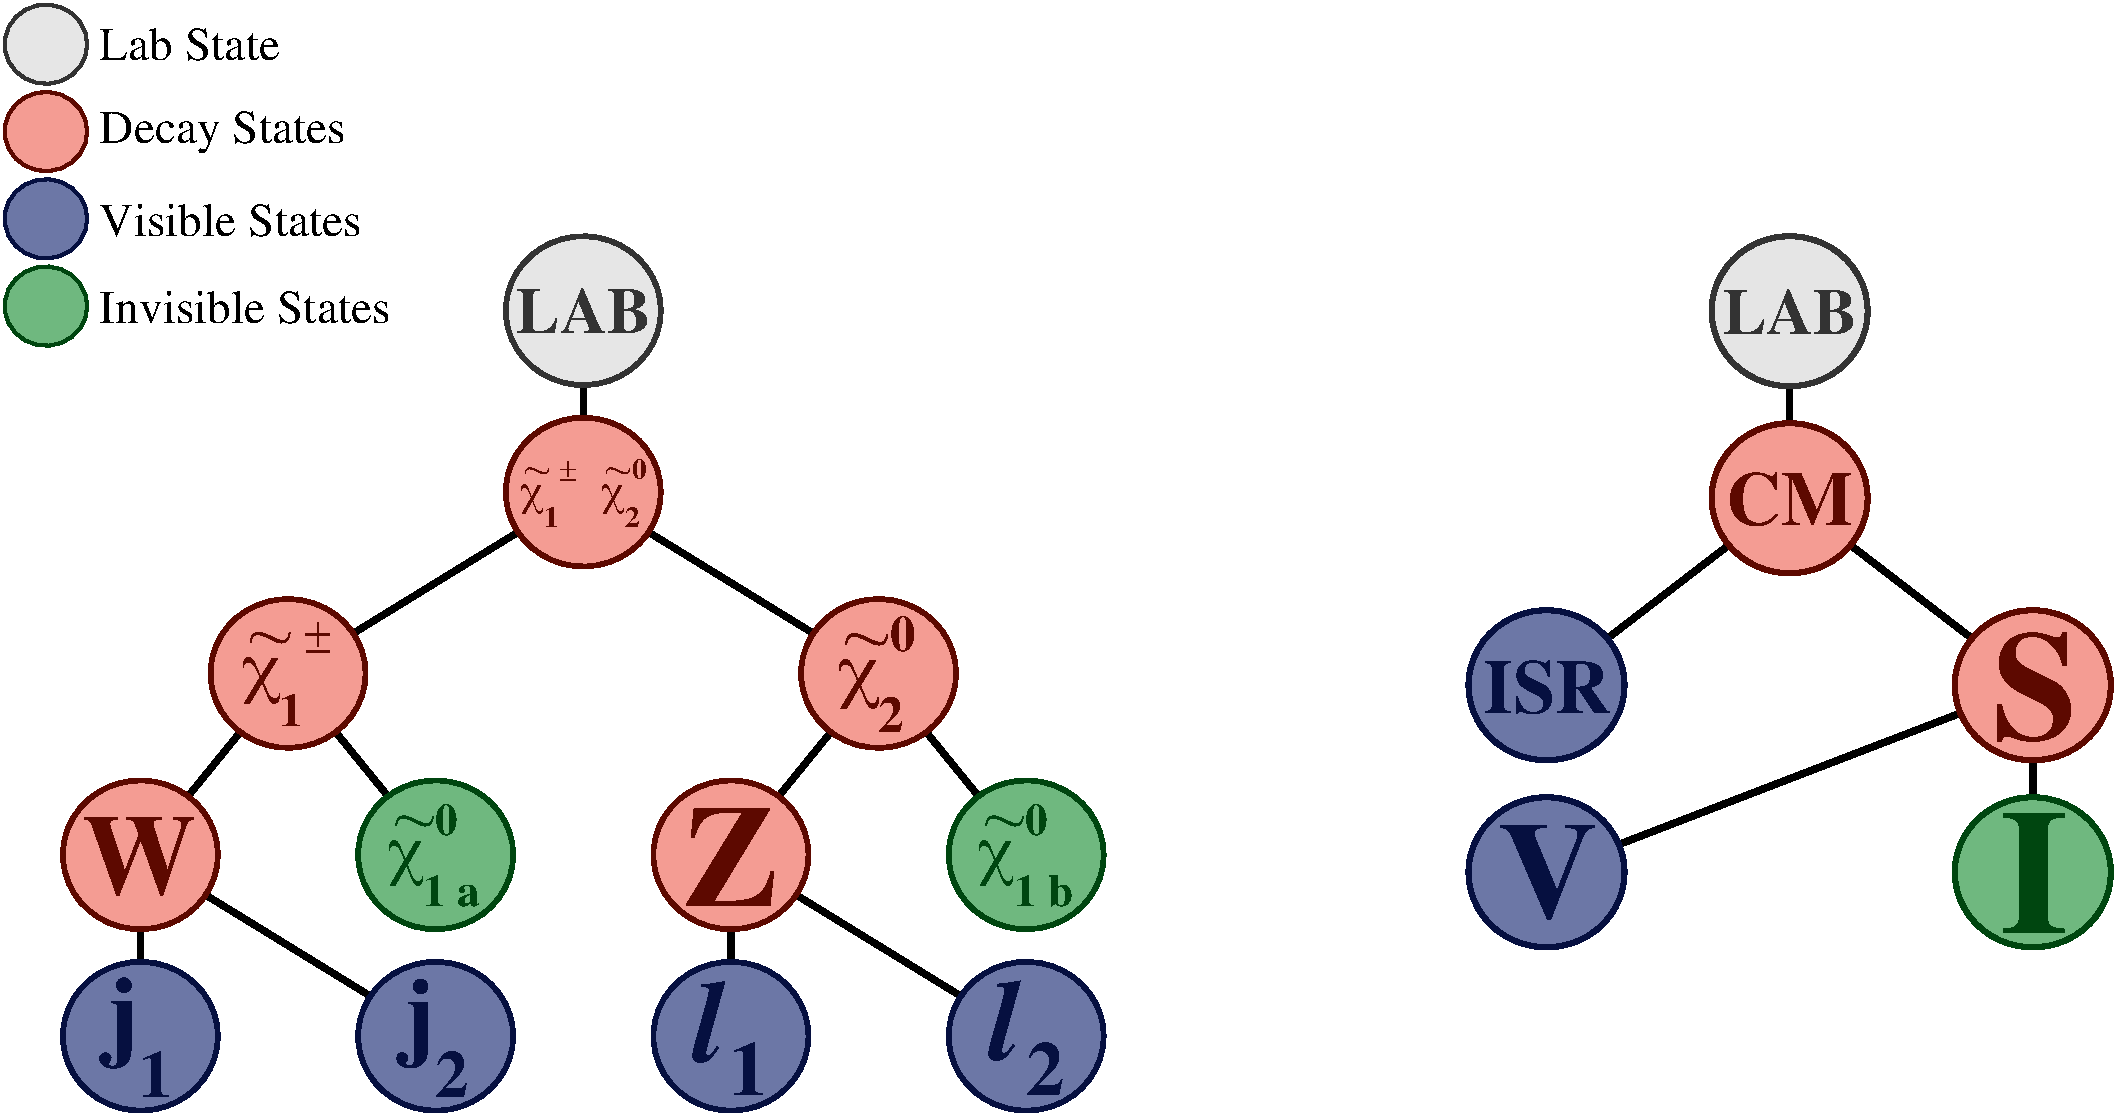
\includegraphics[width=0.9\textwidth]{figures/2ljets_rjr_trees.pdf}
\caption[
Decay trees for the $\twoljets$-RJR analysis
]{%
Decay trees for the $\twoljets$-RJR analysis.
\emph{This figure was made by the RJR team.}~\cite{atlas2022searches}.
Both diagrams represent processes that are targetted in the electroweak
analysis.
(left) A fully-resolved decay tree with its particles labelled.
(right) Only the $Z\to\ell\ell~$ \underline{V}ector boson
is resolved, but the supersymmetric system recoils off
hard QCD jets labelled `ISR' that boost the \underline{I}nvisible system,
to generate visibly large $\met$ in models that would otherwise not,
due to their small mass-splittings.
A similar concept is approached by the SR-OffShell selections in the
$\twoljets$-electroweak search.
}
\label{fig:2ljets_rjr_decay_trees}
\end{figure}


\subsubsection{Former excesses}
Excess data were observed in several signal regions of the past partial Run~2
search ``for chargino-neutralino production using recursive
jigsaw reconstruction in final states with two or three charged
leptons''~\cite{atlas_rjr_23l_SUSY_2017_03},
which used $36.1~\mathrm{fb}^{-1}$ of proton-proton collisions at
$\sqrt{s} = 13\,\eV[T]$.
That search reported notable excesses in four signal regions, of which
two required two charged leptons
($\mathrm{SR}2\ell\_\mathrm{Low}$ and $\mathrm{SR}2\ell\_\mathrm{ISR}$),
and the other two required three
($\mathrm{SR}3\ell\_\mathrm{Low}$ and $\mathrm{SR}3\ell\_\mathrm{ISR}$).
These excesses are visible in their summary plots that we reproduce in
Figures~\ref{fig:2ljets_rjr_summaries_2017_2l}
and~\ref{fig:2ljets_rjr_summaries_2017_3l}.
Although the largest local excess was reported as ``$3.0$ standard deviations'',
which is not particularly large, the pattern of four related regions with
excess data can understandably draw attention.

Both of these three-lepton regions with past excesses,
$\mathrm{SR}3\ell\_\mathrm{Low}$ and $\mathrm{SR}3\ell\_\mathrm{ISR}$,
have been revisited with the full Run~2 data-set and updated background
modelling;
their update sees ``no significant excesses''~\cite{atlas_rjr_3l_SUSY_2019_09}.
These regions have also been approximated without direct use of RJR event
variables;
those approximations also find data ``in agreement'' with background
modelling~\cite{atlas_rjr_mimic_SUSY_2018_06}.

The $\twoljets$-RJR search serves to reproduce
$\mathrm{SR}2\ell\_\mathrm{Low}$ and $\mathrm{SR}2\ell\_\mathrm{ISR}$,
with the full Run~2 data-set and updated background modelling,
and asks whether the excesses persist.
They do not.
As seen in Figure~\ref{fig:2ljets_rjr_summaries_2ljets},
neither reproduced region shows any significant deviation of data from its
fitted background.

\begin{figure}[tp]
\centering
\begin{subfigure}{0.495\textwidth}
\centering
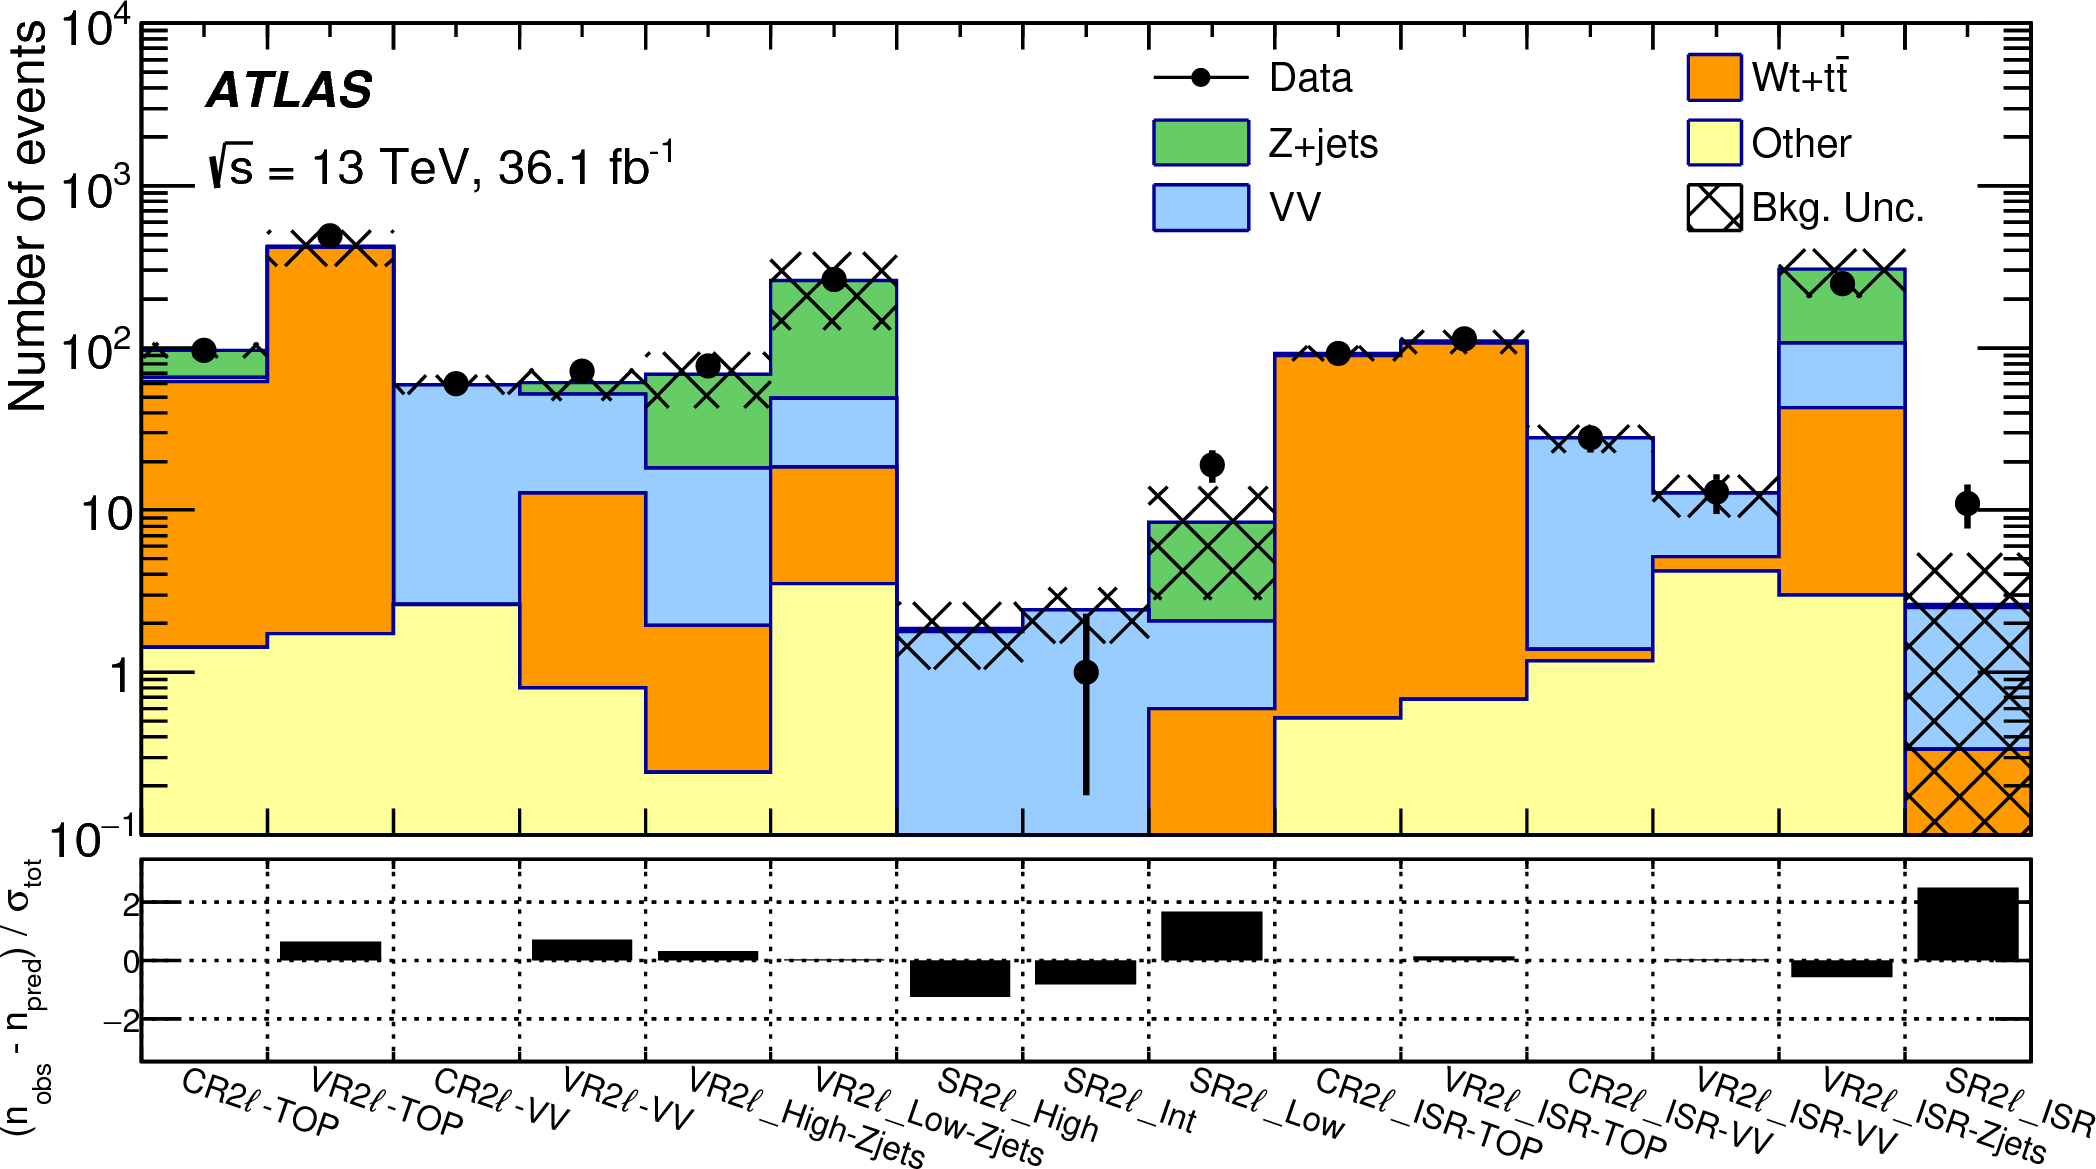
\includegraphics[width=\textwidth]{figures/2ljets_rjr_23l_2l_summary.png}
\caption{$2\ell$ RJR~\cite{atlas_rjr_23l_SUSY_2017_03}}
\label{fig:2ljets_rjr_summaries_2017_2l}
\end{subfigure}
\hfill
\begin{subfigure}{0.495\textwidth}
\centering
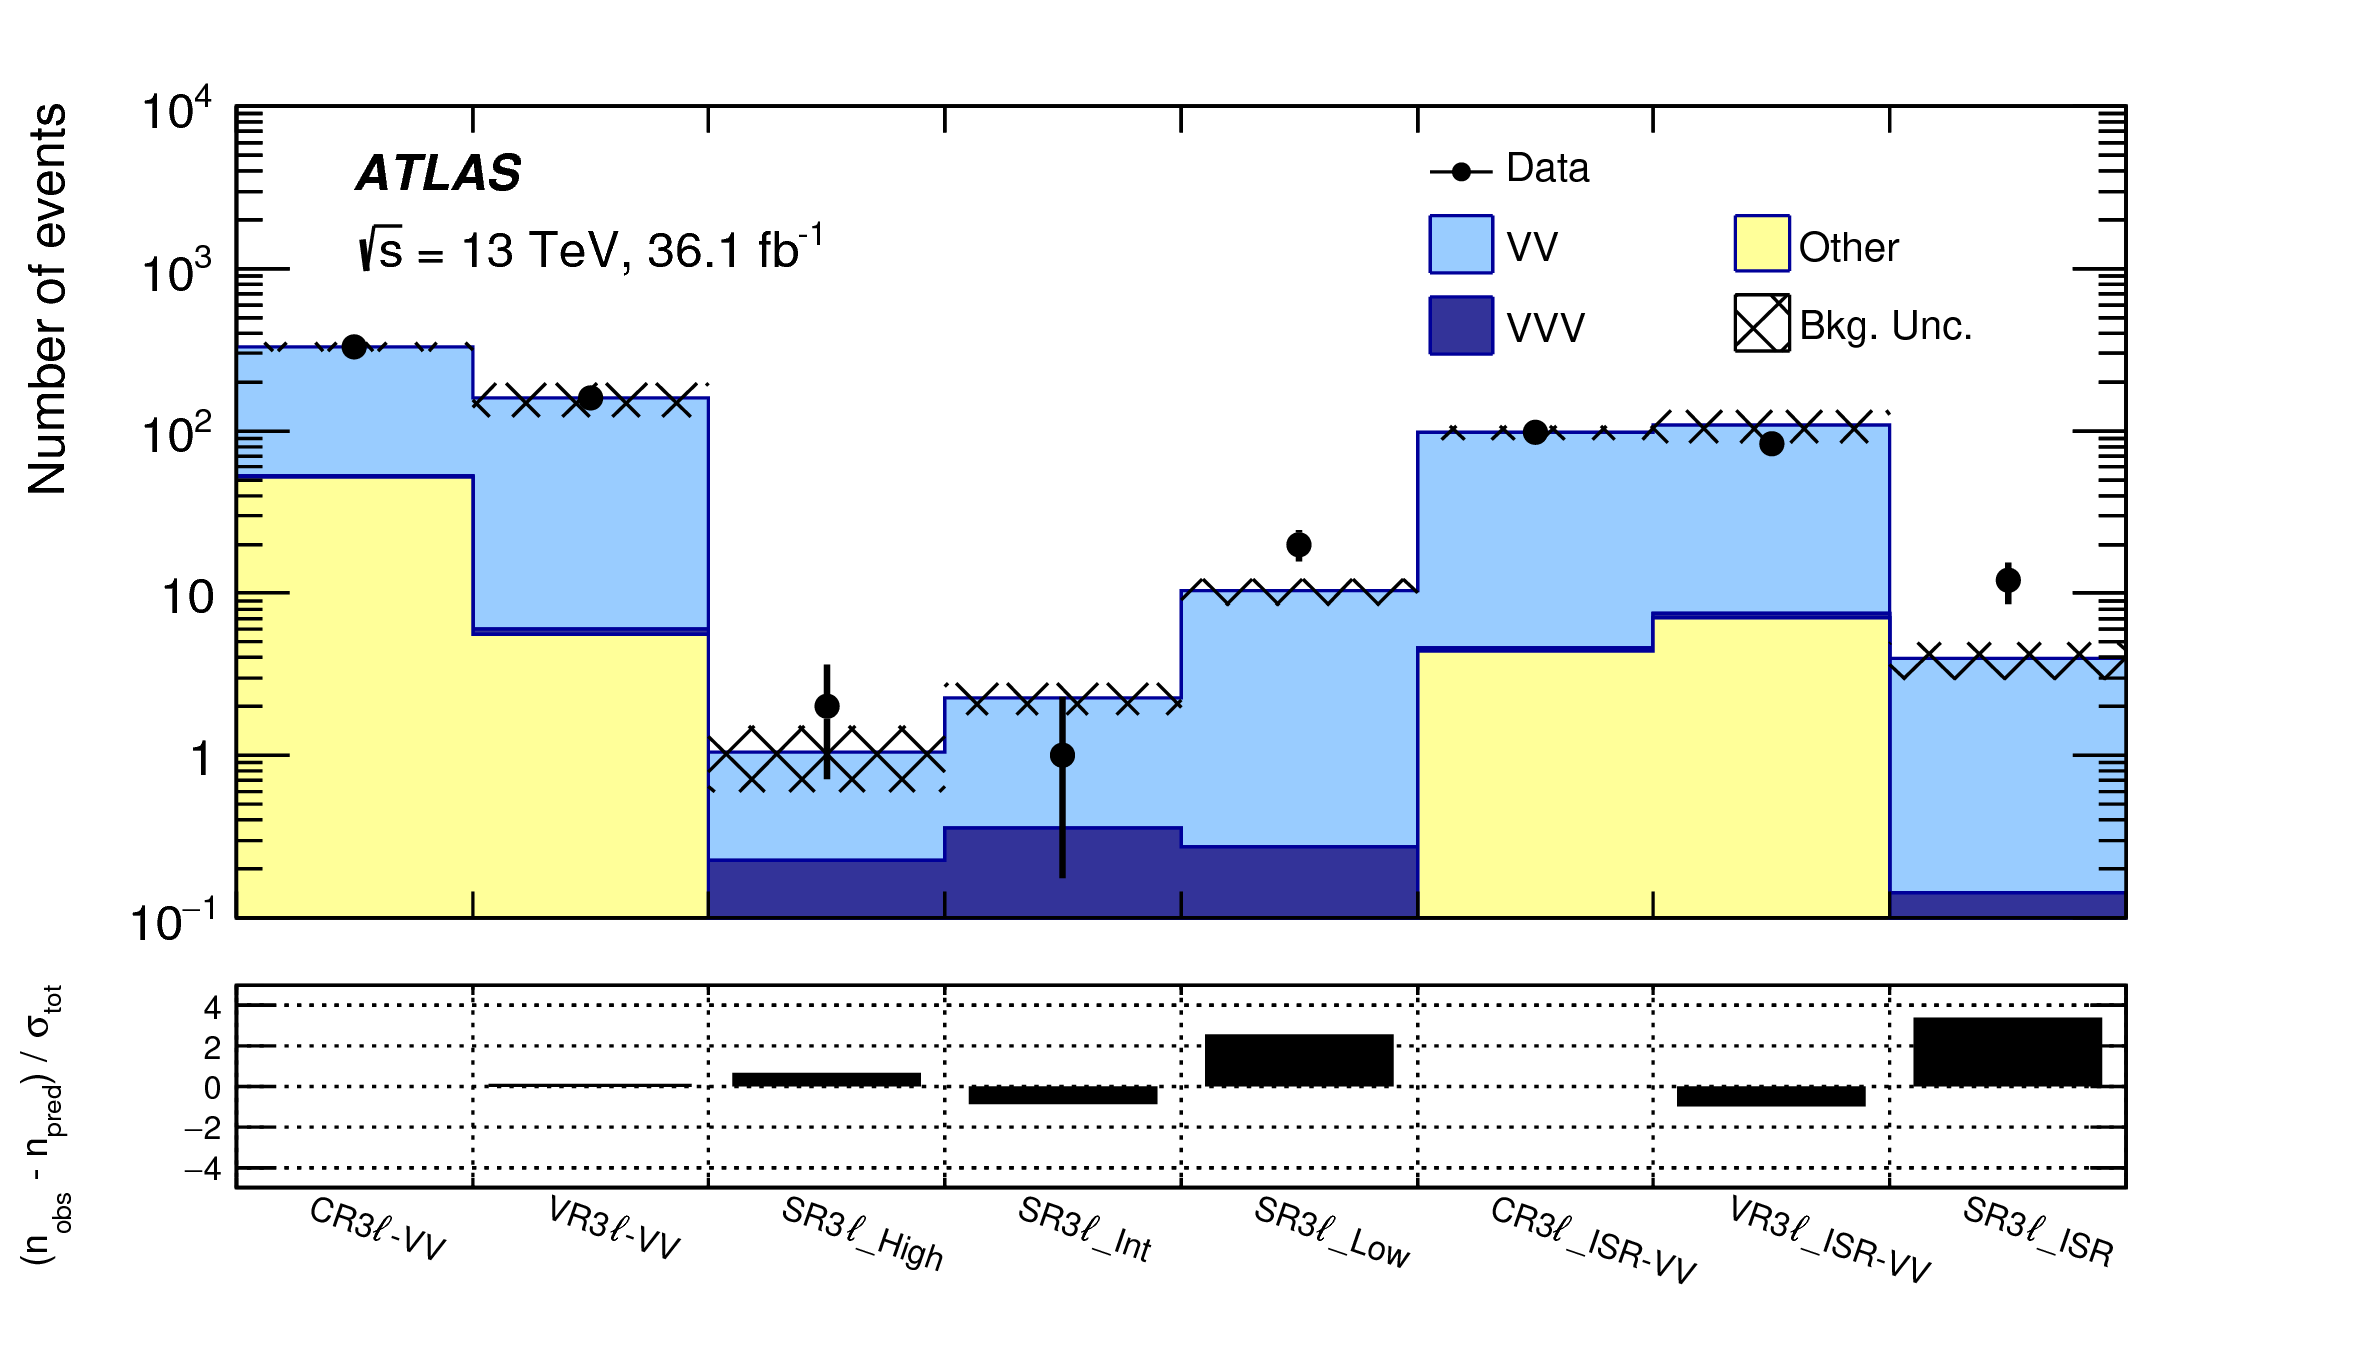
\includegraphics[width=\textwidth]{figures/2ljets_rjr_23l_3l_summary.png}
\caption{$3\ell$ RJR~\cite{atlas_rjr_23l_SUSY_2017_03}}
\label{fig:2ljets_rjr_summaries_2017_3l}
\end{subfigure}
\\[0.4em]
\begin{subfigure}{0.9\textwidth}
\centering
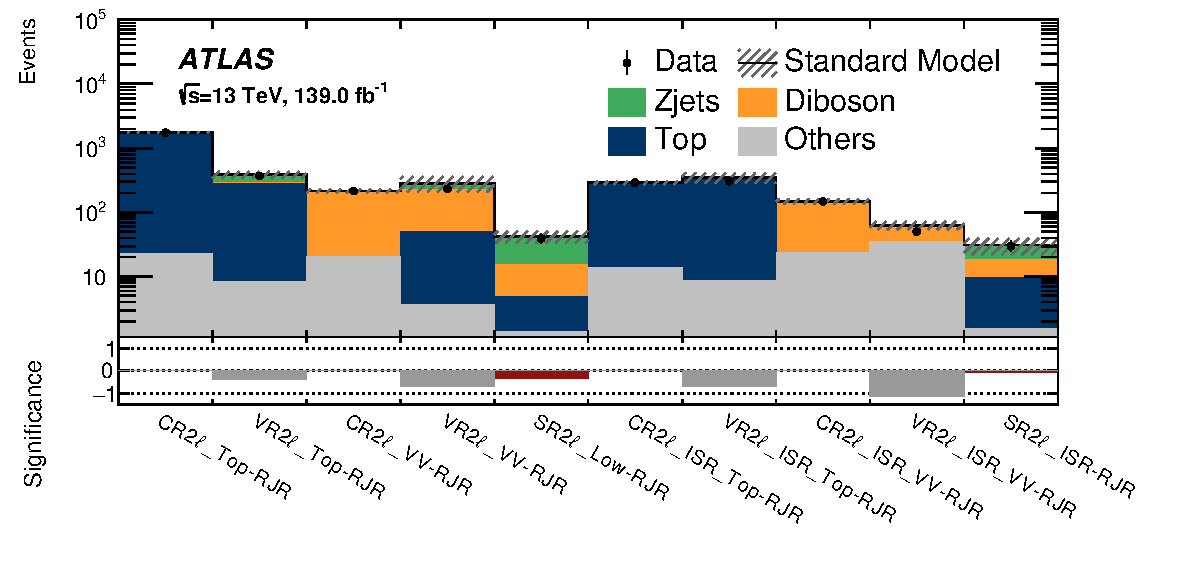
\includegraphics[width=\textwidth]{figures/2ljets_rjr_summary_log.pdf}
\caption{$\twoljets$-RJR~\cite{atlas2022searches}}
\label{fig:2ljets_rjr_summaries_2ljets}
\end{subfigure}
\caption[
Summary plots for RJR searches
]{%
Summary plots for RJR searches:
(a) and (b)~two- and three- lepton selections, respectively,
\emph{reproduced from}~\cite{atlas_rjr_23l_SUSY_2017_03},
(c)~all regions from the $\twoljets$-RJR search~\cite{atlas2022searches}.
Note the excesses in
$\mathrm{SR}2\ell\_\mathrm{Low}$ and $\mathrm{SR}2\ell\_\mathrm{ISR}$ of (a),
and in
$\mathrm{SR}3\ell\_\mathrm{Low}$ and $\mathrm{SR}3\ell\_\mathrm{ISR}$ of (b).
\emph{Sub-figure (c) was made by the RJR team.}
}
\label{fig:2ljets_rjr_summaries}
\end{figure}


\subsubsection{Doubts}
Disappearing excesses have encouraged some doubts about RJR variables in
certain social circles;
the existence of the `RJR-mimic' paper~\cite{atlas_rjr_mimic_SUSY_2018_06},
which approximates the $3$-lepton result of~\cite{atlas_rjr_23l_SUSY_2017_03}
with non-RJR ``laboratory-frame'' event variables,
is public evidence of this.

A more precisely framed problem with RJR variables is that they tend to select
regions of phase space that are poorly modelled by simulations.
This is plausibly explained by the fact that RJR variables are non-trivially
related to conventional, lab-frame variables.
All of our simulations have been tuned to model conventional variables well,
and systematic variations are also evaluated and derived in those conventional
variables.
Unfortunately, modelling the distributions of standard event variables
accurately does not necessarily imply that all other functions of the data are
well modelled.
These effects might contribute to the fact that our Monte Carlo simulations
give predictions in RJR regions that are inaccurate and/or carry large
uncertainties.

A lack of reliable simulations motivates reliance on `data-driven' background
estimates in RJR selections, which, from my perspective, are hard to interpret
or trust.
Indeed,  all `data-driven' methods rely not only on data but on
hypothetical extrapolations that may not be well motivated, particularly when
studying complicated non-linear event variables such as RJR variables.
Although RJR variables can appear to offer appealing separations of
supersymmetric signals from Standard Model backgrounds, these practical issues
motivate my decision to not use any RJR event variables in the
$\twoljets$-electroweak analysis.


\FloatBarrier
\subsection{Strong}
\label{sec:2ljets_origins_strong}
Strongly interacting supersymmetric particles, the super-partners of quarks and
gluons, would be produced at much larger cross-sections than their electroweak
cousins at the LHC.
Squarks and gluinos in simplified models are therefore excluded with masses up
to several $\eV[T]$ using hadronic data alone~\cite{atlas_susy_strong_0l}.

The $\twoljets$-strong search is designed to target strongly interacting
supersymmetric effects in cases where their decays include pairs of charged
leptons.
Like the RJR and electroweak $\twoljets$ searches, signal models targeted by
the $\twoljets$-strong search produce jets and invisible LSPs.
Unlike the RJR and electroweak parts, however, not all of these leptons are
produced by $Z$ boson decays;
as illustrated in Figure~\ref{fig:2ljets_strong_signal_diagrams}, decay trees
featuring sleptons can also produce lepton pairs.
Lepton pairs produced in these slepton interactions are of the same flavour
and opposite charge, like those from $Z$ boson decays, but they have different
dilepton mass characteristics.

\begin{figure}[tp]
\centering
\begin{subfigure}{0.48\textwidth}
\centering
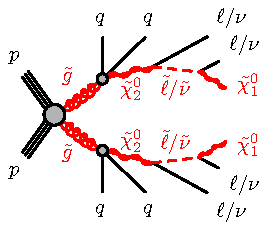
\includegraphics[width=\textwidth]{figures/2ljets_strong_gogo_qqqqllllN1N1_N2.pdf}
\caption{gluino-slepton}
\end{subfigure}
\hfill
\begin{subfigure}{0.47\textwidth}
\centering
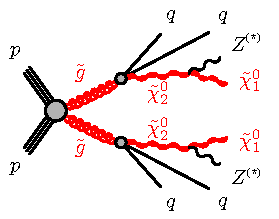
\includegraphics[width=\textwidth]{figures/2ljets_strong_gogo_qqqqZZN1N1.pdf}
\caption{gluino-$Z^{(*)}$}
\end{subfigure}
\\[0.4em]
\begin{subfigure}{0.48\textwidth}
\centering
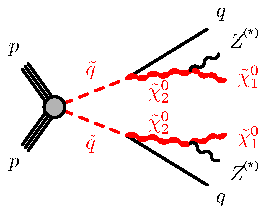
\includegraphics[width=\textwidth]{figures/2ljets_strong_sqsq_qqZZN1N1.pdf}
\caption{squark-$Z^{(*)}$}
\end{subfigure}
\caption[
Diagrams for supersymmetric signal models targeted by the $\twoljets$-strong
search
]{%
Diagrams for supersymmetric signal models targeted by the $\twoljets$-strong
search.
\emph{These figures are reproduced from the paper%
}~\cite{atlas2022searches, atlas_susy_feynman}.
\\[0.4em]
All three produce same-flavour, opposite-sign lepton pairs, along with jets
and $\met$.
The gluino-slepton model (a) has a kinematic endpoint in $\mll$
given in Equation~\ref{eqn:2ljets_strong_max_mll}.
The gluino-$Z^{(*)}$ and squark-$Z^{(*)}$ models decay via $Z$ boson
resonances that may be forced off-shell for small mass-splittings
$m(\neutralino_2) - m(\neutralino_1) < m(Z)$.
}
\label{fig:2ljets_strong_signal_diagrams}
\end{figure}

Rather than peaking at a resonance mass, the lepton pairs in the
`gluino-slepton' signal model have an $\mll$ distribution that features a
signature end-point that depends on the masses of other supersymmetric
particles in the
$\neutralino_2 \ldots\ \slepton \ldots\ \neutralino_1$
decay chain~\cite{paige1996determining}:
\begin{equation}
\label{eqn:2ljets_strong_max_mll}
\max(\mll)
= m(\neutralino_2)
\sqrt{1 - \frac{m(\slepton\,)^2}{m(\neutralino_2)^2}}
\sqrt{1 - \frac{m(\neutralino_1)^2}{m(\slepton\,)^2}}
.
\end{equation}

Previous incarnations of this search have been conducted with similar
selections and signal models in older data, including partial Run~2~\cite{
atlas_susy_strong_2l_partial_run2_1,
atlas_susy_strong_2l_partial_run2,
cms_susy_2016_strong_2l_run2_1,
cms_susy_2016_strong_2l_run2
} and Run~1~\cite{
atlas_susy_strong_2l_run1,
cms_susy_2016_strong_2l_run1
} in \atlas\ and \cms.
From these Run~1 searches, one can cherry-pick excesses
of ``$3.0$ standard deviations'' in \atlas\ \cite{atlas_susy_strong_2l_run1}
and ``$2.6$ standard deviations'' in \cms~\cite{cms_susy_2016_strong_2l_run1}.
These excesses of data above estimated backgrounds were not reproduced in their
early Run~2 updates.

To target its signal models, the $\twoljets$-strong search defines seven
overlapping signal regions.
Three target on-shell $Z^{(*)}$ models by selecting $\mll$ close to
$m(Z)\approx 91.2\,\eV[G]$~\cite{pdg2022ynf},
and the others are binned in $\mll$ for sensitivity to the various
kinematic endpoints that arise across the grid of various signal model
parameters.

The largest Standard Model background to this search is dileptonic $\ttbar$,
partly because it employes no veto for $b$-tagged jets.
All three signal models produce same-flavour lepton pairs, but $\ttbar$
produces same-flavour ($ee$/$\mu\mu$) and different-flavour ($e\mu$) pairs at
equal rates.
The $\twoljets$ search exploits this difference in flavour symmetry to derive
a data-driven background estimate for all of its flavour-symmetric backgrounds,
and have its previous iterations~\cite{cms_susy_2016_strong_2l_run2_1}.
The background estimate works by taking different-flavour data, weighting them
by factors to calibrate for differences in the leptons' reconstruction, and
histogramming them in same-flavour regions.
Simulations for $\ttbar$ and the smaller flavour symmetric backgrounds
$tW$, $WW$, and $\tau\tau$ are replaced by this estimate.

All post-fit results in $\twoljets$-strong regions match the data to within
$1$-sigma.

Exclusion contours from the $\twoljets$-strong search are reproduced in
Figure~\ref{fig:2ljets_strong_contours} and show a substantially increased
area of exclusion, improving by around $400\,\eV[G]$ in the largest limits on
$m(\tilde g)$ over the partial Run~2
results~\cite{atlas_susy_strong_2l_partial_run2}.
However, the jagged edges along these contour are striking.
This jaggedness arises from the method employed to combine exclusion contours
derived from individual signal regions.
Because they overlap, they are not independent and cannot be trivially
combined.
Instead, each model in the signal grid is assigned to the signal region
with the ``best expected sensitivity'' by some
measure~\cite{atlas2022searches}.
This combination method constructs an exclusion contour for each signal region,
then joins those contours such that models assigned to each region use its
corresponding contour.

\begin{figure}[tp]
\centering
\begin{subfigure}{0.62\textwidth}
\centering
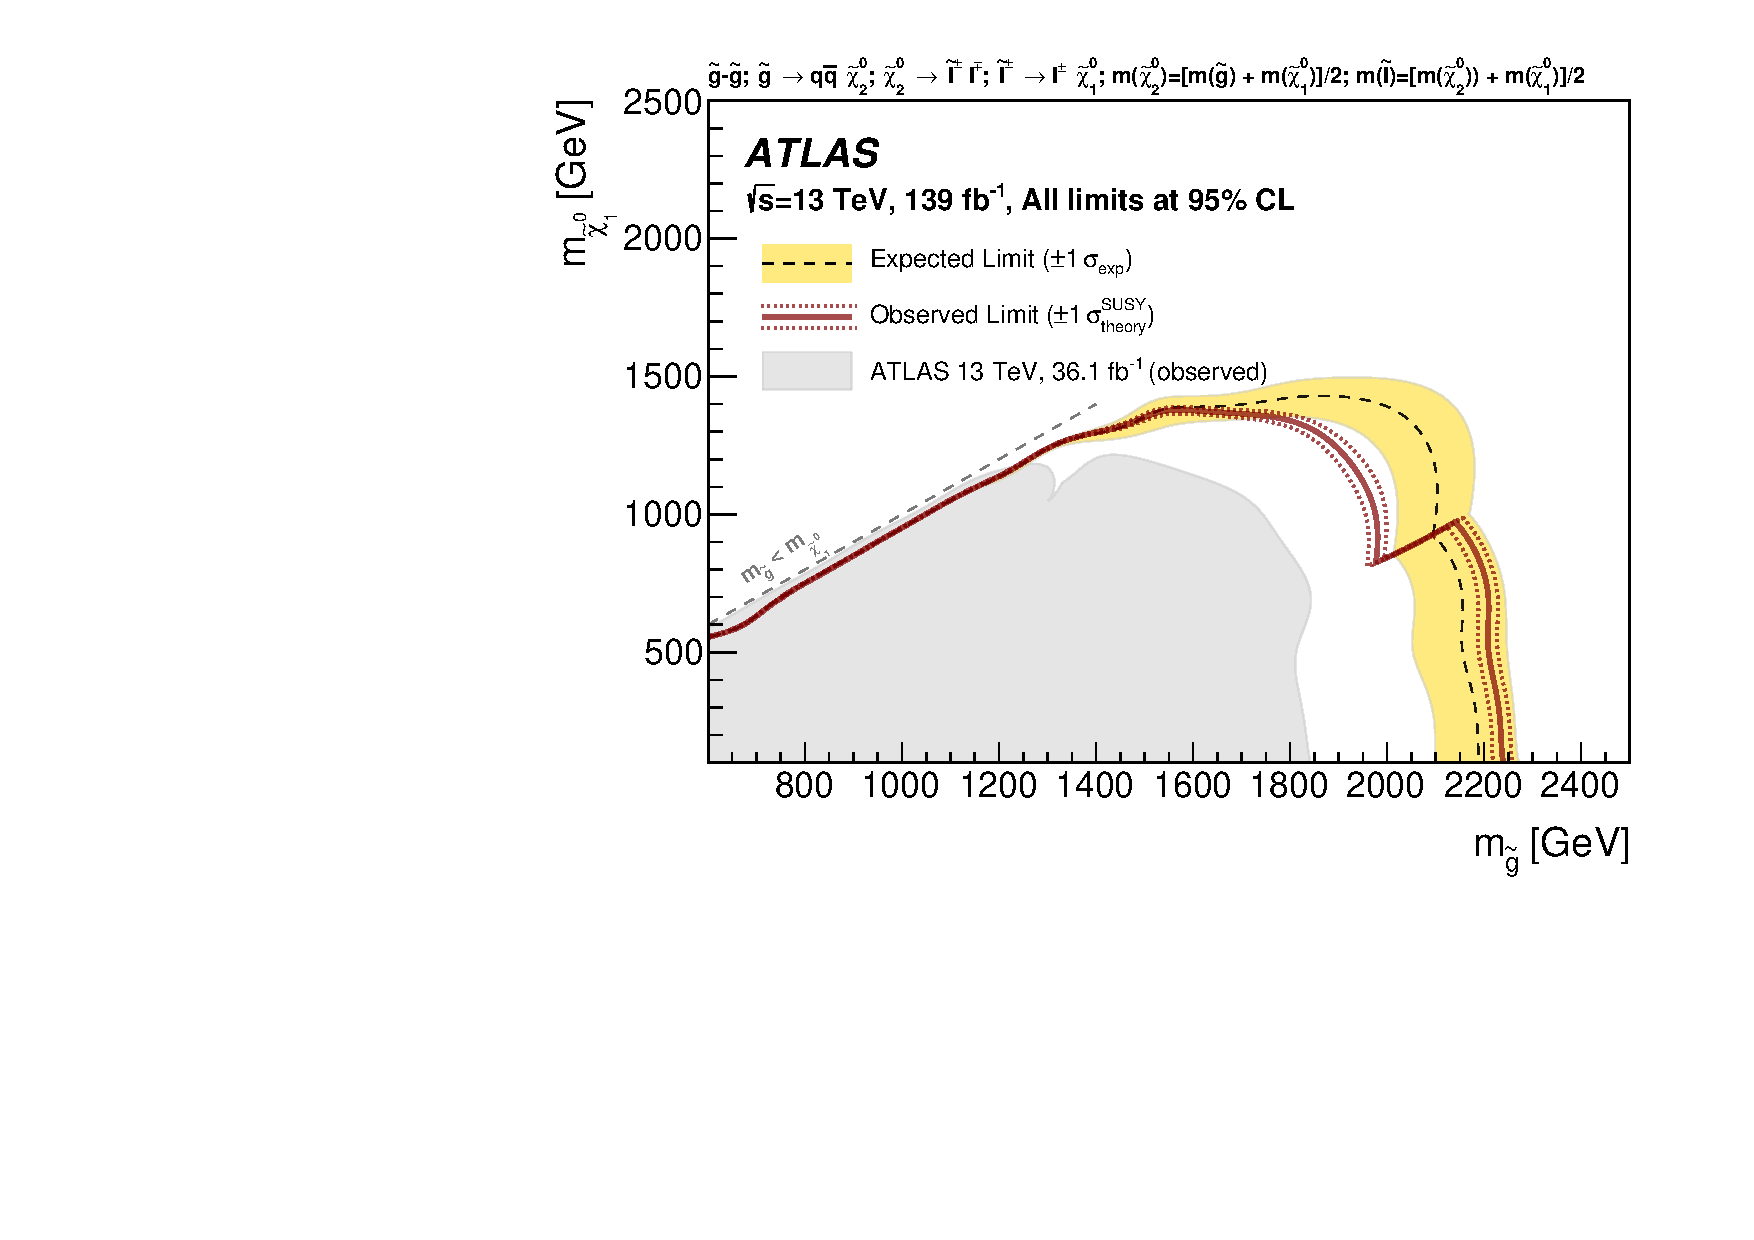
\includegraphics[width=\textwidth]{figures/2ljets_strong_contours_gluino_slepton.pdf}
\end{subfigure}
\\
\begin{subfigure}{0.62\textwidth}
\centering
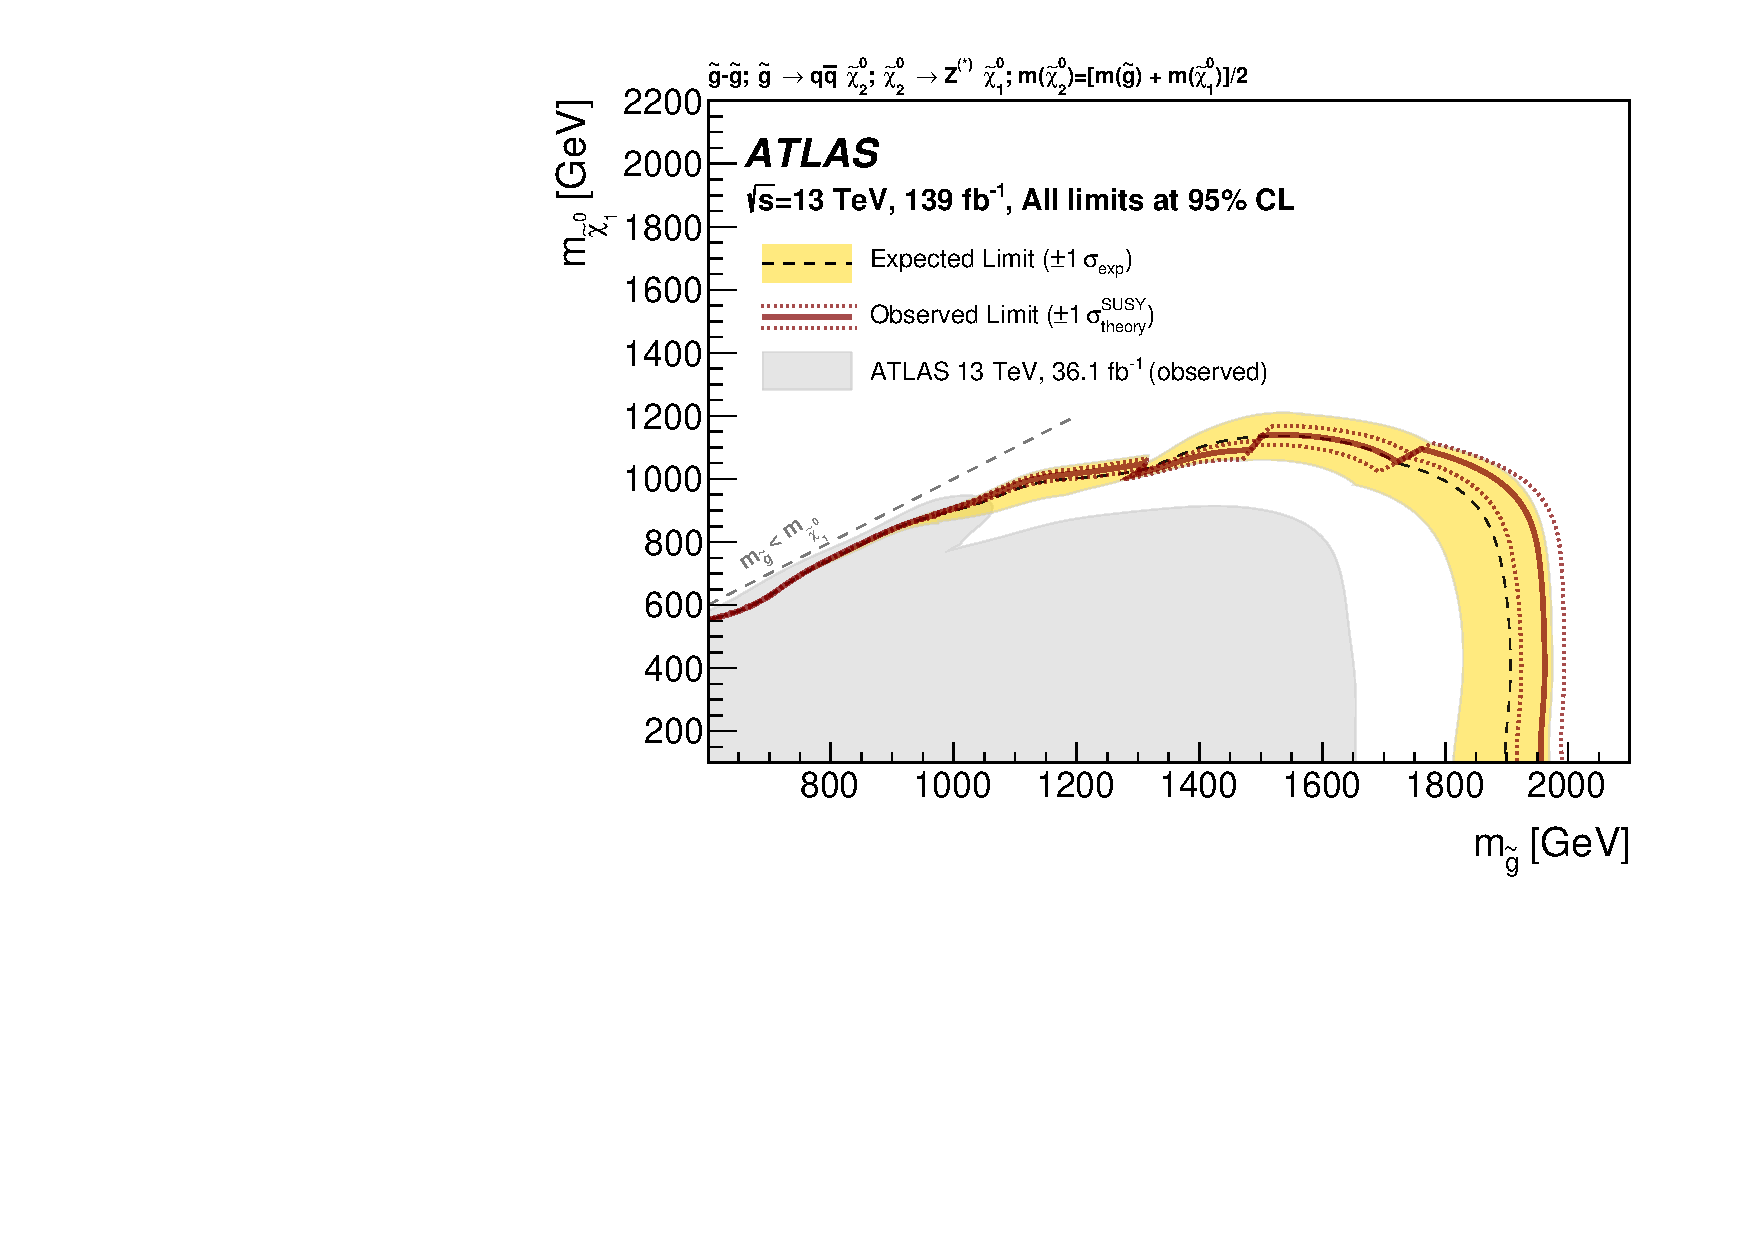
\includegraphics[width=\textwidth]{figures/2ljets_strong_contours_gluino_z.pdf}
\end{subfigure}
\\
\begin{subfigure}{0.62\textwidth}
\centering
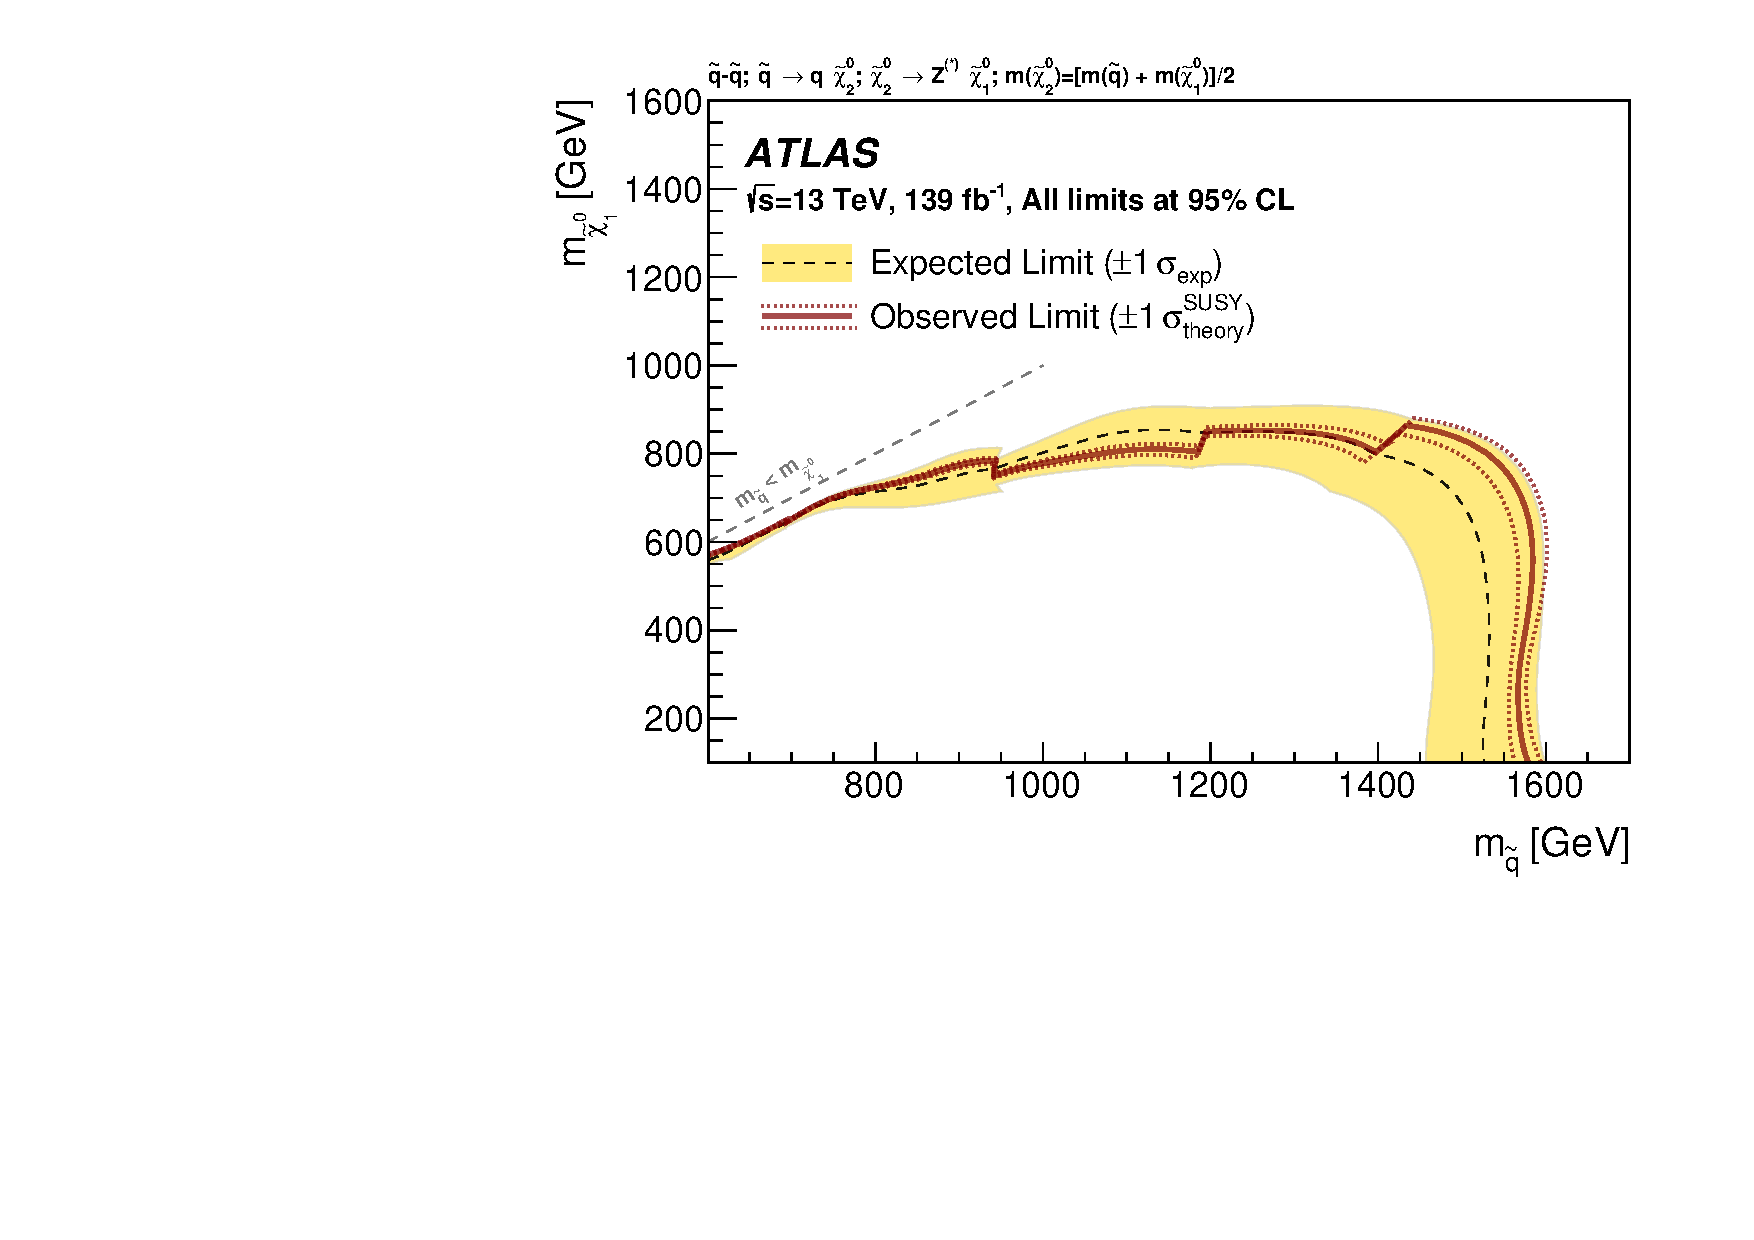
\includegraphics[width=\textwidth]{figures/2ljets_strong_contours_squark_z.pdf}
\end{subfigure}
\caption[
Contours for signal models of the $\twoljets$-strong search
]{%
Contours for signal models of the $\twoljets$-strong search.
\emph{These figures were produced by the strong team%
}~\cite{atlas2022searches}.
\\[0.4em]
(Top) gluino-slepton,
(Middle) gluino-$Z^{(*)}$,
(Bottom) squark-$Z^{(*)}$.
\\
Each model point uses fit results from the signal region with the
``best expected sensitivity'';
jagged edges arise from the switching between contours set by these different
signal regions.
The grey shaded contours showing previous exclusion are taken
from~\cite{atlas_susy_strong_2l_partial_run2}.
No previous contour is available for the exact squark-$Z^{(*)}$ model studied
here.
}
\label{fig:2ljets_strong_contours}
\end{figure}

Personally, I find these jagged contours hard to interpret.
If I were interested in a theory that landed on one of these sharp
region-transition edges, what should I make of these data?
I wouldn't know.
It seems certain that some combination of the regions could have combined their
information to produce a continuous and more informative contour.
Where model predictions change continuously in these signal spaces, it seems
that our inferences should also.
To aid interpretations and to allow justifiable combinations of regions'
information, I therefore chose to design the $\twoljets$-electroweak with only
orthogonal regions, and without any switching of regions between models.


\subsection{Electroweak}
\label{sec:2ljets_origins_electroweak}
As motivated in the previous sections, I have personal preferences for
simulation-driven backgrounds and orthogonal multi-bin regions.
Simulation-driven estimates are interpretable as Standard Model predictions,
relying less on loosely justified extrapolations,
and orthogonal regions have independent Poisson likelihood functions that can
be cleanly combined, by multiplication, to leverage the joint information in
their data.

The $\twoljets$-electroweak search aims to
update the regions of the partial Run~2 search in its $\twoljets$
channel~\cite{atlas_23l_SUSY_2016_24}, which also searched for the same C1N2
signal models that produce chargino-neutralino pairs decaying via $W$ and $Z$
bosons.
A particular design goal was to improve sensitivity by replacing their overlapping
`SR2-int' and `SR2-high' regions with orthogonal selections.
\emph{Special thanks to Sarah~Williams for suggesting this approach.}

Similarly to the $\twoljets$-strong search, the partial Run~2
search~\cite{atlas_23l_SUSY_2016_24} chose one signal region for each signal
point from an expected sensitivity measure, and drew contours around
results from the chosen fit results.
The two signal regions SR2-int and SR2-high differ only by a selection of
$\met > 250\,\eV[G]$ and are displayed in Figure~\ref{fig:2ljets_23l_stuff},
along with the combined exclusion contour (additionally including an `SR2-low'
region and a three-lepton result) and the map of which region is chosen at
which signal point.

\begin{figure}[tp]
\centering
\begin{subfigure}{0.62\textwidth}
\centering
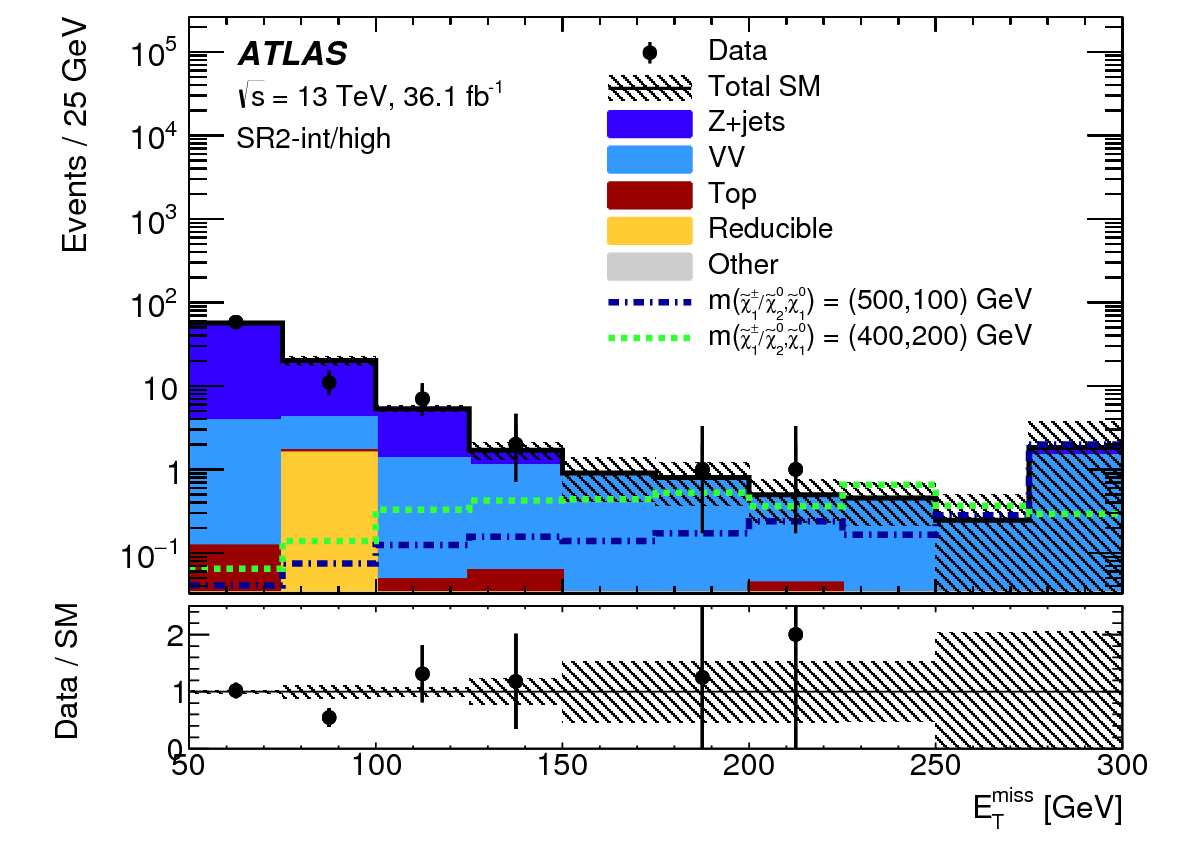
\includegraphics[width=\textwidth]{figures/2ljets_23l_sr2inthigh.png}
\caption{SR2-int and SR2-high}
\end{subfigure}
\\[0.4em]
\begin{subfigure}{0.525\textwidth}
\centering
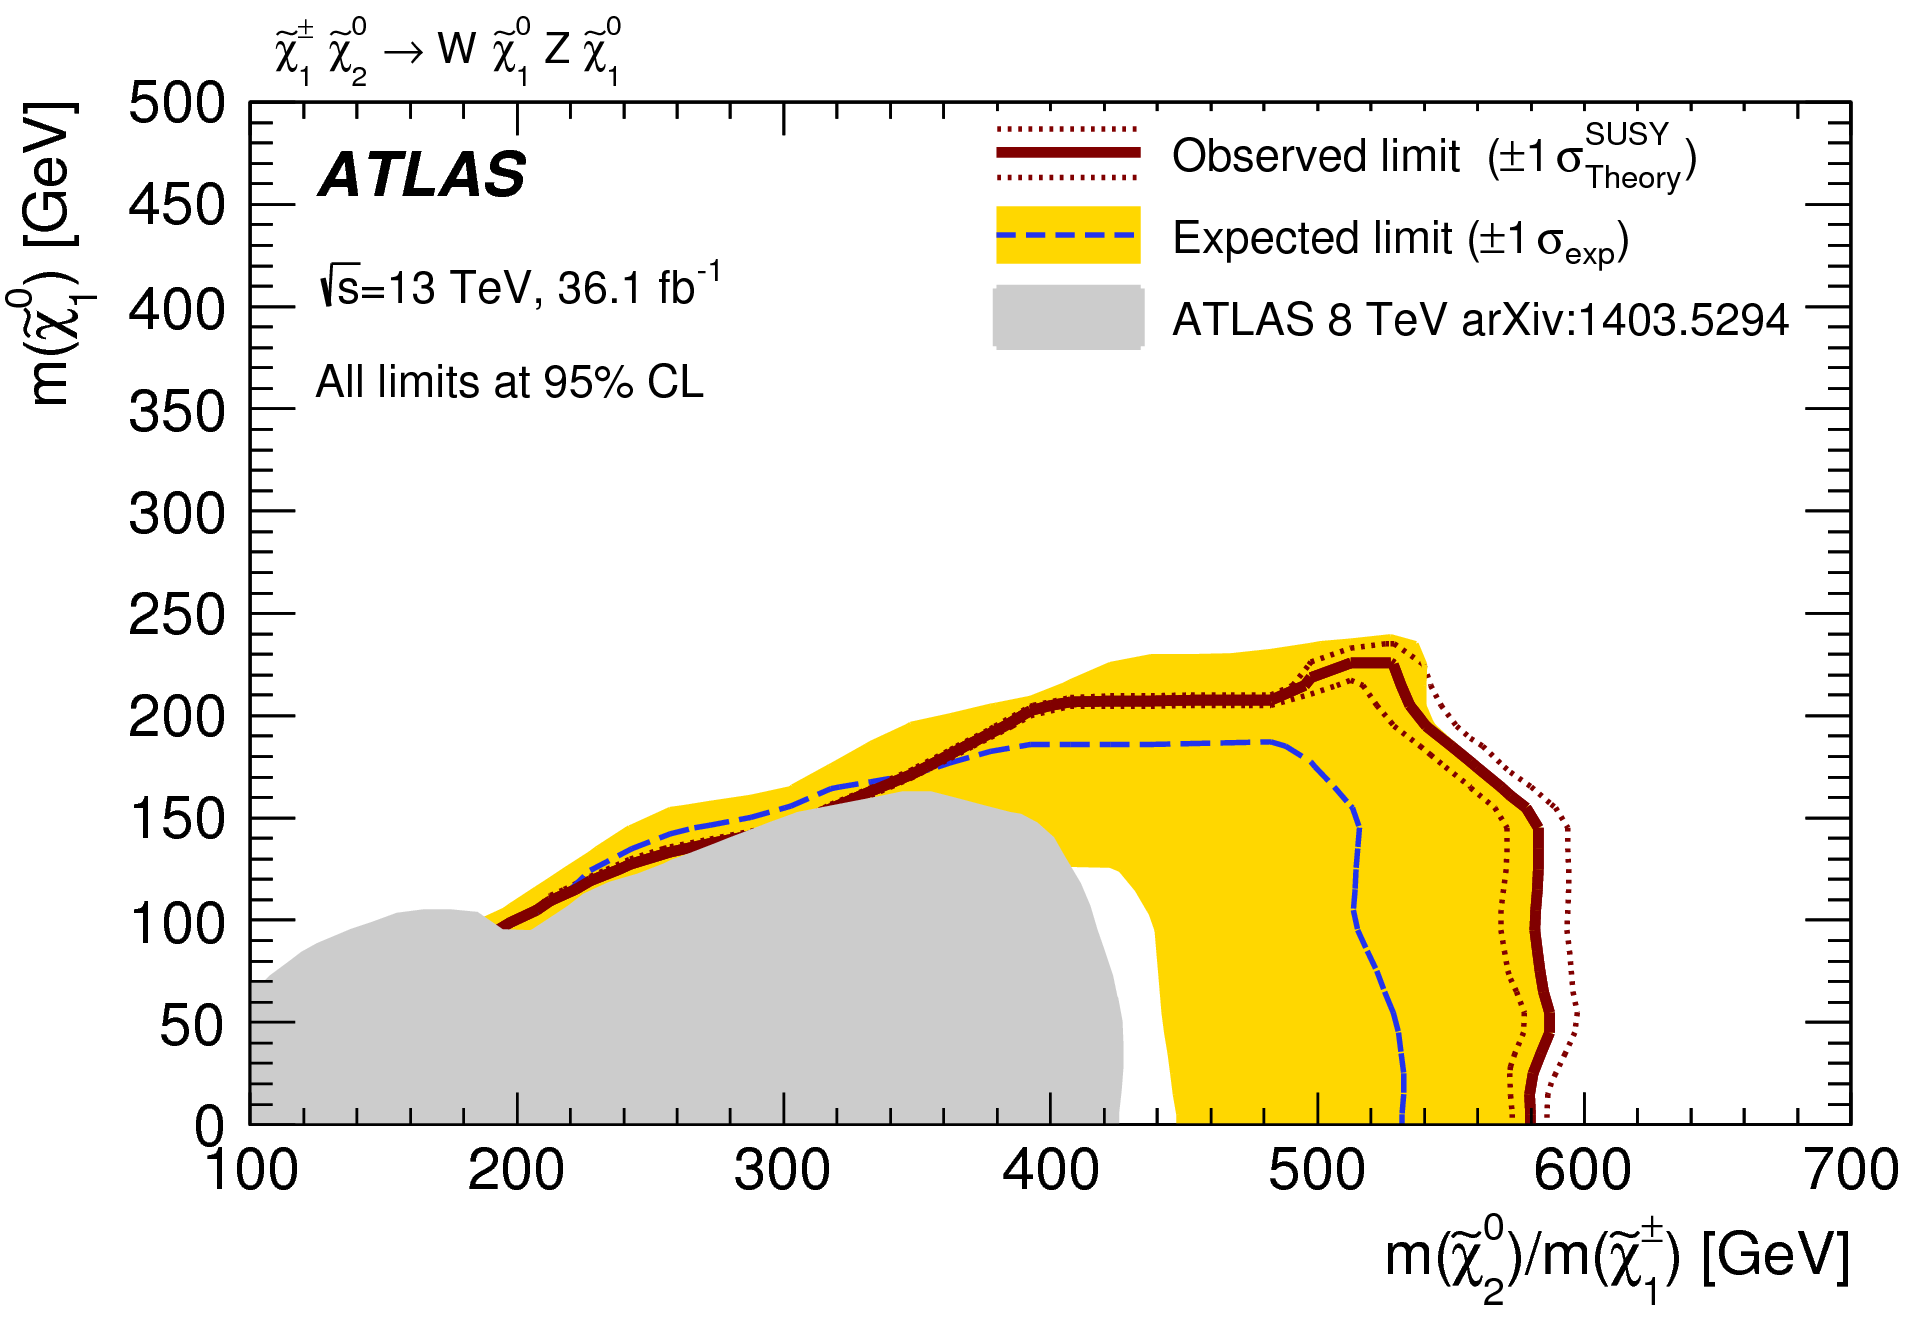
\includegraphics[width=\textwidth]{figures/2ljets_23l_contours_fig_08d.png}
\caption{Combined exclusion}
\end{subfigure}
% \hfill
\begin{subfigure}{0.465\textwidth}
\centering
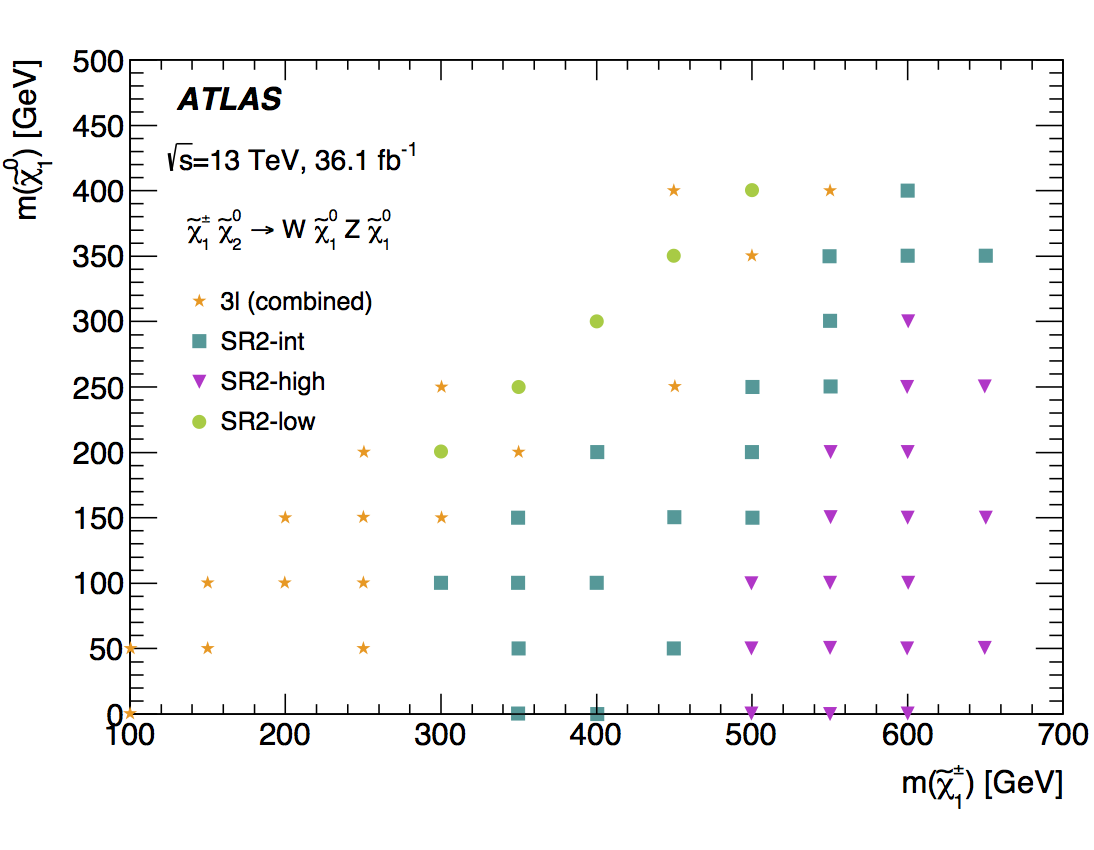
\includegraphics[width=\textwidth]{figures/2ljets_23l_chosen_regions.png}
\caption{Chosen regions}
\end{subfigure}
\caption[
Figures reproduced from the partial Run~2 search with $2/3\ell$ selections
]{%
Figures reproduced from the partial Run~2 search with $2/3\ell$
selections~\cite{atlas_23l_SUSY_2016_24, hepdata.81996}.
The event variable $\met$ is the missing transverse momentum.
The label $m(\chargino_1)/m(\neutralino_2)$ indicates the mass
$m(\chargino_1, \neutralino_2)$ under the simplifying assumption that
$m(\chargino_1, \neutralino_2) = m(\chargino_1) = m(\neutralino_2)$.
\\[0.4em]
(a) Histogrammed distribution of $\met$ in and below SR2-int and SR2-high with
example signal models.
SR2-int requires $\met > 150\,\eV[G]$ and SR2-high requires $\met > 250\,\eV[G]$.
\\[0.4em]
(b) Contours for the combined $\twoljets$ and $3\ell$ channels.
Each signal point chooses a signal region, which is displayed in (c).
The grey region shows exclusion from a previous search in Run~1
data~\cite{atlas_2l_SUSY_2013_11}.
\\[0.4em]
(c) Signal regions selected for each signal point in the grid.
Two-lepton selections occupy the largest mass-splittings.
The $3\ell$ regions are orthogonal and combined.
}
\label{fig:2ljets_23l_stuff}
\end{figure}

Additionally, $\twoljets$ widens its scope to target a GMSB simplified model
that is illustrated in Figure~\ref{fig:2ljets_signal_diagrams}.
The C1N2 and GMSB models behave similarly since both feature gaugino decays via
massive bosons ($W\kern-0.4exZ$, $ZZ$ or $Zh$) to leptons and jets, in
similarly structures decay trees to invisible supersymmetric pairs.
Although widening sensitivity to both models must sacrifice some sensitivity to
each individually, the increased degree of model independence is itself of
value for future reinterpretations of our data.
We are happy to sacrifice some precision for generality.
Since the $W$ and $Z$ boson masses are similar, this sacrifice turned out to
have quite a minor impact.

Multi-bin fits are not special.
They are standard \atlas\ practice, and there should have been no complication
had I imitated SR2-int and SR2-high for $\twoljets$-electroweak, but with minor
tweaks to change them into orthogonally binned regions.
However, my design decisions for $\twoljets$-electroweak became much more
ambitious, increasing to a total of $13$ signal regions with complicated
definitions.
Although this multi-bin design squeezed out some extra sensitivity,
it also caused problems --- for the clarity of communication and the accuracy
of our background modelling;
these issues shall be developed throughout the remainder of this chapter.

A multi-binned histogram is usually and clearly illustrated as slicing up one
variable.
My design of $\twoljets$-electroweak violates this.
Instead, it is designed more like a tree whose branches recursively split
various variables.
This leads to specifications that are challenging to present or understand,
and which require region names with numerous suffixes to specify where they
live in that tree.

Worse, I disregarded the popular idea that every region should have a large
background expectation, preferably of ten events or more.
This requirement is typically justified by the limitations of approximate
statistical methods which work
``from as few as $\mathcal{O}(10)$ data events''~\cite{baak2015histfitter}.
But the Poisson likelihood works for infinitesimally small
expectations~\cite{skilling2009cosmology}, and in the small-bin limit one has
continuous of `unbinned' distributions with Poisson normalizations
(sometimes called ``extended'' in High-Energy
Physics~\cite{barlow1990extended})
that are standard elsewhere in High-Energy Physics,
and are easily analysed by the standard likelihood fitting
methods~\cite{cowan1998statistical}.
Examples uses of unbinned modelling include analyses of hadronic
resonances in
\lhcb~\cite{Tullythesis,lhcb2018563}, searches for exotic effects in
\atlas~\cite{EXOT-2018-08},
and notably the observation of the
Higgs boson~\cite{HIGG-2012-27}.

Events appearing in a region with minimal background is evidence in favour
of new contributions, and that only strengthens as the background approaches
zero.
For example, the top quark was observed by \dzero\ using seven regions all with
background expectations of one event or less, for a total of $3.79\pm0.55$
expected and seventeen observed~\cite{abachi1995observation}.
If they could do that with technology from the year $1995$, we can do it now.
This is a fact, but only if we can really trust our predictions of zero
backgrounds.

The real reason to avoid small backgrounds is, in this context, to allow honest
assignments of background uncertainties.
Although main simulated samples may have good precision,
many variations for systematic uncertainties and data-driven estimates are also
required.
Many methods to evaluate these variations have far worse precision than the
central simulations, and can fail totally as their number of Monte Carlo events
accepted plunges towards zero.
In practice, our methods to assign background uncertainties can easily require
tens of expected events to work properly.

Unfortunately, the $\twoljets$-electroweak regions designs were finalized
before unblinding, and before I appreciated this problem with background
uncertainties in the smaller regions.
Various workarounds are therefore invoked to assign plausible variations
despite small yields and failing statistical precision, which shall be seen in
the remainder of this chapter.
As seen in the splash summary of Section~\ref{sec:2ljets_splash}, the
$\twoljets$-electroweak search observes agreement with post-fit backgrounds
except for some local deficits of data below backgrounds.
Exclusion contours exceed their expected range because of these deficits,
but they can only be trusted if the background model is trusted.

The \cms\ Collaboration has published similar searches for
C1N2~\cite{cms_susy_2022_c1n2} and GMSB models~\cite{
cms_susy_2018_partial_run2_combination,
cms_susy_2022_gmsb
}, with comparable exclusion limits in similar selections of data.
Other published \atlas\ results in the full Run~2 dataset put constraints on
the same models that we study in $\twoljets$.
Since we designed these searches to use orthogonal datasets, they may be
combined for more sensitive future results.

For the C1N2 model, these public Run~2 \atlas\ searches explore the
all-hadronic~\cite{SUSY-2018-41},
$2\ell/3\ell$ compressed~\cite{atlas_susy_compressed_2l_2018_run2},
$3\ell$ on-shell~\cite{SUSY-2018-06}, and
$3\ell$/same-sign~\cite{SUSY-2018-09} channels.
In comparison to these other searches, our exclusion contour of
Figure~\ref{fig:2ljets_contours_c1n2} excludes a unique area of parameter
space within $m(\chargino_1,\neutralino_2) \in 550\textrm{--}700\,\eV[G]$
and $m(\neutralino_1) \in 200\textrm{--}300\,\eV[G]$.
The all-hadronic search is most sensitive at the highest parent masses,
and three-lepton data of in the on-shell and compressed searches are most
sensitive at intermediate and small (off-shell/compressed) mass splittings.

For the GMSB model, our result complements limits from the
$4\ell$~\cite{SUSY-2018-02} and
all-hadronic~\cite{SUSY-2018-41} searches.
In addition to the exclusion contours that we present in
Figure~\ref{fig:2ljets_contours_gmsb}, the all-hadronic search again dominates
the heaviest parameter space, with $m(\neutralino_1) > 600\,\eV[G]$,
and the $4\ell$ search has more sensitivity at
$m(\neutralino_1) < 250\,\eV[G]$.
This leaves the area that our $\twoljets$-electroweak search uniquely excludes
to have with large Higgs branching fractions (up to $90\%$) at intermediate
masses with $m(\neutralino_1) \in 250\textrm{--}600\,\eV[G]$.
Exclusion of the largest $B(\neutralino_1 \to h \tilde{G})$ values
requires sensitivity to double-Higgs decay signatures --- \cms\ have published
exclusions in the region combining $hh\to \gamma\gamma+\met$ and
$hh\to b\bar bb\bar b$ with other channels to exclude
$B(\neutralino_1 \to h \tilde{G}) = 1$ up to
$m(\neutralino_1) = 750\,\eV[G]$~\cite{
cms_susy_2018_partial_run2_combination,
CMS-SUS-16-045,
CMS-SUS-16-044
}.

For reasons described in this section, the $\twoljets$-electroweak search is
designed with large number of orthogonal regions, and with those regions its
results offer some extensions over previous and orthogonal constraints.
Before describing those regions' definitions and modelling we apply to their
expected yields, the following sections now return to the basic details of the
data and event variables they use.

\section{Events}
\label{sec:2ljets_events}
This section describes the events selected for the three $\twoljets$ searches,
the reconstructed particle objects derived from those events, and various
important event variables.
Definitions of the $\twoljets$-electroweak event variables are collected
Section~\ref{sec:2ljets_cheatsheet}, which is intended as a useful bookmark
for future reminders, and may also clarify occasions where we make forward
references to variables before giving their precise definitions.

The `$\twoljets$' name is intended to indicate interest in events with two
charged leptons (those are electrons or muons --- not taus), and at least one
jet.
Though not in the name, an $\met$ requirement is also implicit from the context
of $R$-parity conserving supersymmetric models.
This Section~\ref{sec:2ljets_events} serves to describe how events are selected
for the $\twoljets$ searches, and which event variables are extracted for use
in its selections.

Our dataset comprises $139.0\,\mathrm{fb}^{-1}$ ($\pm 1.7\%$) of integrated
luminosity observed during normal operations of the \atlas\ detector in the
years $2015$ through to $2018$ of the LHC Run~2~\cite{DAPR-2018-01}.
Triggers and object definitions are shared between the three $\twoljets$
searches.
Higher level event variables and selections will only be described here for the
$\twoljets$-electroweak search.


\subsection{Trigger}
\label{sec:2ljets_trigger}
There would be no event variables without events, and \atlas\ only records
when triggered.
When living our lives as humans, we are bombarded with sensory data and must
pay attention only to those few gems of any use, to avoid exhausting our
processing capacity.
Running \atlas\ is no different --- its triggering is necessary to reduce the
bombardment of collision data to a manageable size.

Each trigger in \atlas's arsenal activates on a selection comprising some
combination of sufficiently hard objects.
The set of targeted objects includes all those used in this analysis and more:
electrons, muons, jets, $b$-jets, $\met$, as well as photons and hadronically
decaying tau leptons~\cite{atlas2008experiment}.

The list of available triggers in \atlas\ is designed to balance data rates
against physical interest.
It includes a variety of general purpose selections, which are used for
$\twoljets$, along with more specialized targets such as vector boson fusion
or long-lived particles.
That trigger list has varied through time, so we select triggers individually
in each data-taking period.

The loosest triggers are `prescaled', meaning that their data rate is reduced
by randomly accepting only a small fraction of events.
Interpreting prescaled data adds some complications that we avoid in
$\twoljets$, by using only un-prescaled triggers.
We use only the `lowest' (loosest, highest rate) triggers that select two
charged leptons~\cite{atlas_twiki_lowest_unprescaled}.
Those charged leptons are selected in the high-level trigger,
described in Section~\ref{sec:atlas_trigger}, which
primarily requires large $\pt$ and certain quality criteria.

In total, we use $14$ different two-lepton trigger selections, each of which
selects for an electron pair, a muon pair, or an emu (electron-muon pair).
To describe those triggers, we use $\pt^{\ell_i}$ for the transverse momentum
of the $i\mathrm{th}$ hardest lepton.
All triggers require $\pt^{\ell_i}$ values to exceed thresholds in
the range $8\textrm{--}26\,\eV[G]$.
To detail all trigger requirements and their variations with data period
would be too tedious and not enlightening, but their $\pt^{\ell_i}$ requirements
are summarized here.
Please do not read them all in detail ---
the point of this listing is to show trigger activations are varied and
non-trivial.
\begin{itemize}
\item Electron pair: requirements vary between $\pt^{e_2} > 12\,\eV[G]$ and
$\pt^{e_2} > 17\,\eV[G]$.
\item Muon pair: various requirements include
$\pt^{\mu_2} > 10\,\eV[G]$,
$\pt^{\mu_2} > 14\,\eV[G]$,
$\pt^{\mu_1} > 18\,\eV[G]~\&~\pt^{\mu_2} > 8\,\eV[G]$, and
$\pt^{\mu_1} > 22\,\eV[G]~\&~\pt^{\mu_2} > 8\,\eV[G]$.
\item Emu pair: various asymmetric requirements include
$\pt^{e_1} > 17\,\eV[G]~\&~\pt^{\mu_1} > 14\,\eV[G]$,
$\pt^{e_1} > 7\,\eV[G]~\&~\pt^{\mu_1} > 24\,\eV[G]$, and
$\pt^{e_1} > 26\,\eV[G]~\&~\pt^{\mu_1} > 8\,\eV[G]$.
\end{itemize}
Trigger requirements have increased in hardness with time throughout the data
used in $\twoljets$.

This complicated collection of trigger requirements motivates lepton selections
that exceed these trigger thresholds,
such that they avoid the need to accurately model their jagged activation
thresholds and varying efficiencies near to those thresholds~\cite{
atlas_trigger_egamma_run2,
atlas_trigger_muon_run2
}.
To avoid the most of these thresholds, all leptons selected for the
$\twoljets$-electroweak regions are required to have $\pt > 25\,\eV[G]$.


\subsubsection{Alternative triggers}
Why should we only use two-lepton triggers?
Alternatives could be one-lepton triggers, for cases where the other is not
reconstructed at trigger level, or perhaps also triggers for jets and $\met$.
The answer is that the benefits of additional triggers were assessed to not
outweigh the cost of using them.

The benefit of an additional trigger could be in increased signal yields if
that trigger does not also harmfully increase inseparable backgrounds.
A study, \emph{performed by Knut~Vadla}, investigated the effects
of including one-lepton triggers.
In a signal-region-like selection requiring two leptons, two jets and
$\met > 200\,\eV[G]$, this study showed that two-lepton triggers already accept
in excess of $90\%$ of events from benchmark C1N2 models.
Therefore, any additional trigger has at most a $10\%$ improvement.
Adding one-lepton triggers was found to increase acceptance rates by only a
few percentage points.
Especially since this must come with a comparable increase in background rates,
the benefit is too little to be considered worthwhile.

Costs of triggers are primarily attributable to human effort:
software work to include them and their associated Monte Carlo weights, and
extra studies to validate background estimates and evaluate systematic
uncertainties.
Similarly, our implementation of the Matrix Method fake/non-prompt lepton
background estimate (described in Section~\ref{sec:2ljets_mm_fakes}) is not
equipped to handle one-lepton triggers, so further work would have been
required to replace it.

Although jet and $\met$ triggers were not studied in detail, they can be
quickly ruled out since they only trigger on hard objects:
examples of these triggers require
approximately $\ptjone > 400\,\eV[G]$, $p_\mathrm{T}^{\,j_3} > 200\,\eV[G]$, or
$\met > 100\,\eV[G]$~\cite{atlas_twiki_lowest_unprescaled}.
Leptons, however, are striking signals that are produced at smaller
background rates, as they are suppressed by electroweak couplings.
\atlas\ can therefore trigger on leptons with much softer requirements;
lepton triggers allow us to use softer jets and $\met$, which are relied upon
throughout the $\twoljets$ analyses.
Although $\twoljets$-electroweak requires $\met > 100\,\eV[G]$ in all of its
regions, the same is not true of $\twoljets$-RJR, nor various validation
studies.


\subsection{Leptons}
\label{sec:2ljets_events_leptons}
As mentioned at the beginning of this Section~\ref{sec:2ljets_events},
`leptons' means `electron-or-muons' in the context of $\twoljets$.
This is because taus leptons decay before reconstruction so are used only
indirectly through their decay products, and neutral leptons
--- neutrinos --- go missing and contribute only to our $\ptmiss$.

Reconstructed lepton objects feature momenta, charges, and flavours.
Each lepton is accepted for use in $\twoljets$ only if it satisfies certain
kinematic selections and is identified with `quality' criteria.
For both electron and muons, these criteria are standardized with labels
`loose', `medium', and `tight';
these labels are nested in the sense that tight implies medium
and medium implies loose.
Other, more specialized, criteria exist in \atlas, but they are not relevant
to $\twoljets$.

Muons are identified by fitting tracks to hits in the inner tracker and muon
spectrometer.
Their quality criteria use goodness-of-fit metrics from those fits, along with
low-level details of detector interactions.
Tighter requirements primarily act to reduce from non-prompt backgrounds,
which are muons from hadronic decays~\cite{atlas_muon_quality_MUON_2018_03}.

Electron identification combines data from the inner tracker and
calorimeters.
Electron quality criteria use numerous features of detector
interactions, track fitting metrics, the matching of tracks to calorimeter
clusters, calorimeter shower shapes, and leakage into the hadronic calorimeter.
Tighter requirements reduce backgrounds, which include misidentified objects
--- photons and hadrons --- as well as non-prompt electrons from hadronic
decays~\cite{atlas_egamma_quality_EGAM_2018_01}.

Isolation of leptons from nearby hadronic activity is another feature that
can be used to reduce misidentification rates.
Standard isolation definitions exist for both electrons and muons in a similar
structure to the quality criteria.

Leptons in $\twoljets$ are further sliced into two classes:
`baseline' and `signal'.
Baseline leptons and are used in background estimation methods and to ensure
orthogonality with other \atlas\ analyses that study events with differing
lepton counts, such that our results can be combined in future to deliver an
improved total sensitivity.
Baseline requirements are softer and lower quality than signal requirements;
the signal leptons are a subset of the baseline leptons.
Therefore if a lepton is a signal lepton, then it is also a baseline lepton,
but for clarity we often prefer to state that both requirements are met.

Any event used in regions of the $\twoljets$-electroweak analysis is required
to have exactly two baseline leptons and exactly two signal leptons, meaning
that the event has two reconstructed leptons that pass both sets of criteria.
Requiring exactly two baseline leptons ensures that we veto events with soft
or low quality third leptons, thus ensuring that our data do not overlap with
other \atlas\ analysis that use three-lepton events.
Enforcing no overlap in this way makes the analysis more independent, and
therefore amenable to cleaner combinations in future meta-analyses.

Baseline leptons must have $\pt > 3\,\eV[G]$ for muons and
$\pt > 4.5\,\eV[G]$ for electrons.
Signal leptons must have $\pt > 10\,\eV[G]$, along with tighter
quality and isolation requirements, details of which are given in the
paper~\cite{atlas2022searches}.
Electrons are accepted within $|\eta| < 2.47$.
Baseline muons have $|\eta| < 2.7$, and signal muons have $|\eta| < 2.6$.

All leptons used in regions of the $\twoljets$-electroweak analysis are signal
leptons with $\pt > 25\,\eV[G]$.
This harder requirement reduces backgrounds, moves our selections away from the
lowest trigger thresholds, and matches the precedent set by previous
work~\cite{atlas_23l_SUSY_2016_24}.


\subsection{Jets}
Like leptons, hadronic jets are identified with `baseline' and `signal'
requirements, with increasingly tight requirements on quality metrics and
kinematics.

Jets in $\twoljets$ are constructed with the anti-$k_t$ algorithm with a
standard small radius parameter of $R=0.4$~\cite{jet_anti_kt}.
Jets are formed from `topological' clusters of energy deposits in the
calorimeters~\cite{atlas_jet_topo_PERF_2014_07}.

This topological clustering algorithm is no longer the \atlas-recommended jet
algorithm; it has been supplanted in recent years by a `particle flow' method
that uses tracking information to improve the reconstruction of charged
hadrons~\cite{atlas_jet_pflow_PERF_2015_09}.
We did not attempt to switch to these improved jets because the change in
recommendation occurred during the years this analysis was in development, and
the change would have required more work and further delays for an unknown,
but probably small, benefit.

Baseline jets are defined to require $\pt > 20\,\eV[G]$ with $|\eta| < 2.8$;
signal jets additionally require $\pt > 30\,\eV[G]$.
To reduce the impact of pile-up jets, a variety of quality criteria are used,
depending on the jet $\pt$ and $|\eta|$.
Details of these quality criteria and angular selections are given in the
paper~\cite{atlas2022searches}.


\subsection{\textit{b}-jets}
\label{sec:2ljets_btagging}
Tagging adds labels to objects.
Unlike lepton flavour tagging, which can very cleanly separate electrons from
muons, jet tagging is a rather more noisy affair due to \atlas's limited
ability to reconstruct the individual hadrons within jets.
Taggers are available for various jet properties, such charm flavour ($c$-jet),
bottom flavour ($b$-jet).
Of these, $\twoljets$ uses only $b$-tagging, which is particularly useful to
reject $\ttbar$ events and select for $h\to b\bar b$ decays.

Larger radius jets can also use taggers for heavy decays, such as those from
$W$, Higgs or top resonance~\cite{JETM-2018-06}, but large radius jets were
considered too much additional work to be used in $\twoljets$,
particularly since they would require a large set of independently evaluated
systematic variations in addition to those on our standard jets.

Jets originating from $b$ quarks are distinct due to the long lifetimes and
long decay trees of $B$-hadrons, both of which leave signals in \atlas'
inner trackers.
For jets in $\twoljets$, $b$-tagging is useful to separate events due to
$\ttbar$ backgrounds (since their weak decays almost always produce $b$
quarks), and to select for signals producing $Z/h \to b\bar b$ decays
in the GMSB model.

Signal $b$-jets in $\twoljets$ require $\pt > 20\,\eV[G]$, $|\eta| < 2.5$ and a
tag from the `\textsc{MV2c10}' algorithm~\cite{
friedman2002stochastic,
atlas_jet_mv2c10_2017,
atlas_jet_tagging_2019
} at its $77\%$ efficiency working point.
Notice that this $\pt > 20\,\eV[G]$ requirement is softer than our standard jet
selection of $\pt > 30\,\eV[G]$. Selections that veto $b$-tags therefore act on
a softer collection of jets.

This \textsc{MV2c10} algorithm uses a boosted decision tree that is trained on
a mixture of simulated $\ttbar$ and $\zjets$ data.
The reported efficiency means that a true $b$-jet sampled from the
algorithm's testing dataset has an estimated $77\%$ probability of being
tagged.
It uses low-level event variables, including basic kinematics and more intricate
features of reconstructed hadronic decay
trees~\cite{atlas_jet_mv2c10_2017, atlas_twiki_mv2}.

Alternative working points of $70\%$ and $85\%$ efficiency are used in similar
\atlas\ searches;
these alternatives were trialled and found to make negligible differences in
$\twoljets$.

An alternative $b$-tagging algorithm named `DL1' is now recommended by \atlas,
but its performance is ``similar'' to MV2, and the two tag
``highly correlated'' samples~\cite{atlas_jet_tagging_2019}, so we did not
attempt to switch.


\subsection{Overlap removal}
\label{sec:2ljets_overlap_removal}
Leptons and jets are independently reconstructed.
This means that, despite the various quality and isolation requirement, there
can remain examples where detector responses can be attributed to more than
one object.
For example, a track could be attributed to both a muon and an electron,
or a calorimeter energy cluster could be attributed to both an electron and a
photon. Although we do not directly use photons in $\twoljets$, we do not veto
events containing them --- photons are accounted for in the momentum balance
of $\ptmiss$.

Once we know about all the reconstructed leptons and hadronic jets, we can
also improve our rejection of non-prompt leptons from hadron decays by
leveraging the tendency for those non-prompt leptons to be near to jets.
To remove duplicates and further reduce non-prompt lepton contributions, we
apply a standard overlap-removal procedure.
This procedure, which is detailed in the $\twoljets$
paper~\cite{atlas2022searches},
comprises a sequence of rules that modify the collection of event objects.
Some rules decide which object to keep from an overlapping pair,
and others remove leptons overlapping with jets based on their $\Delta R$
and $\pt$.

This sequential overlap procedure is described as follows:
\begin{enumerate}
\item Remove any electron candidate that shares an inner-detector track with a
baseline muon.
This reduces backgrounds from events with
$\mu\to\mu\gamma$, $\gamma\to e^+ e^-$ radiations in the detector.
\item Remove any baseline jet within $\Delta R \leq 0.2$ of a baseline electron.
\item Remove any electron within
$\Delta R \leq \min(0.04 + (10\,\eV[G]) / p_T^e, 0.4)$
of a baseline jet.
This suppresses backgrounds from heavy-flavour hadron decays.
\item Remove any baseline jet that is within $\Delta R \leq 0.2$ of a baseline
muon, or that shares a track with a muon.
\item Remove any muon within
$\Delta R \leq \min(0.04 + (10\,\eV[G]) / p_T^\mu, 0.4)$
of a baseline jet.
This is matches the electron removal instruction above.
\end{enumerate}
The $\ptmiss$ calculation also ignores any electron that shares a calorimeter
cluster with a photon~\cite{atlas2022searches}.


\subsection{\texorpdfstring{$\met$}{ETmiss}}
Every event has $\ptmiss$.
Unlike leptons, jets, and other objects that we must select for, the $\ptmiss$
of an event is a natural result of the conservation of momentum, which \atlas'
barrel-shaped construction allows us to measure with reasonable precision.

The magnitude of $\ptmiss$ is $\met$, pronounced `met'.
Note that despite its $E$, $\met$ is not an energy; transverse energy does not exist.
One may, of course, define a directed `transverse energy', but it will
not be conserved (in the Standard Model) unless it is equivalent to a conserved
momentum.
Indeed, momentum-balanced events do have energy imbalances;
for example, in a $Z\mathrm{+jet}$ event $pp \to Zg$, with the $Z$ and
$g$ emitted back-to-back in the transverse plane with equal momenta
$p = |\pm \vec p|$, the two particles have different energies since they
have different masses: $E_Z^2 = m(Z)^2 + p^2$, $E_g^2 = 0 + p^2$.
% hobbyhorse

The $\ptmiss$ vector is defined such that the vector sum of $\ptmiss$ with
all reconstructed objects, after overlap removal, has zero transverse momentum.
In addition to the leptons and jets used directly in $\twoljets$, this includes
photons, tau leptons, and a `soft term' comprising tracks not associated to
any other objects~\cite{atlas_met}.

All signal models in $\twoljets$ generate hard, invisible particles.
By selecting for large $\met$, however, we select events with either
real invisible particles or bad mismeasurements.
And the rate of badly measured events from Standard Model processes with large
cross-sections can be substantial.
A standard selection requirement in $\twoljets$-electroweak is
$\met > 100\,\eV[G]$.
This is a nice round number (in these conventional units), and corresponds
roughly to where the $\met$-less background $\zjets$ tails off,
and also corresponds roughly to several standard deviations of
a typical $\met$ noise scale of approximately $10\textrm{--}30\,\eV[G]$.
(I observe that noise scale by inspecting $\met / \metsig$ in
$\twoljets$-electroweak selections, where $\metsig$ is defined in the next
section.)


\subsection{\texorpdfstring{$\met$}{ETmiss} significance}
\label{sec:2ljets_metsig}
Most common Standard Model processes at the LHC do not produce hard,
invisible particles.
Our supersymmetric signals, however, do.
This makes the missing transverse momentum $\ptmiss$ and its magnitude $\met$
important features for separating signal and background events in all parts
of the $\twoljets$ search.

The experimental resolution of $\ptmiss$, however, is imprecise, and
importantly varies significantly from one event to another.

A muon, for example, will tend to have its momentum measured more precisely
than a jet of similar energy.
But there are exceptions, and exceptions to the exceptions.
One exception, as discussed in Chapter~\ref{chapter:experiment}, is if the muon
is hard enough that its curvature through \atlas's magnetic fields is
imprecisely reconstructed.
A further exception to that rule can occur, however, if the jet originates from
a $b$ quark, such that the weak decays of its hadrons tend to lose momentum in
neutrinos or soft muons that are not reconstructed.

By incorporating an uncertainty in $\ptmiss$ tailored to each event, the
variable $\metsig$ helps to separate those events with real and well-measured
$\met$ from those where the measured $\ptmiss$ is more likely to result from
mismeasurements.
(The $\metsig$ variable used in this analysis is not directly
aware of $b$-tagging information, but perhaps it could benefit from some.)

In the context of $\twoljets$ selections, $\metsig$ suppresses $\ttbar$
contributions more than $\met$ alone, plausibly because $\ttbar$ events are
accompanied by more hadronic activity than other sources of $\ptmiss$.
This effect in the $\metsig$ distribution is demonstrated in simulations in
Figure~\ref{fig:2ljets_presel_met}.
What remains of the Standard Model in the high-$\metsig$ tail of $\twoljets$
selections is almost pure \diboson\ --- $ZZ$ with a hard $Z\to \nu\nu$,
and $W^\pm Z$ where the charged lepton in $W^\pm\to\ell^\pm\nu$
is not reconstructed; these subcomponents of the \diboson\ process are
discussed later in Section~\ref{sec:2ljets_validation} and displayed in
Figure~\ref{fig:2ljets_splits_diboson}.

\begin{figure}[tp]
\centering
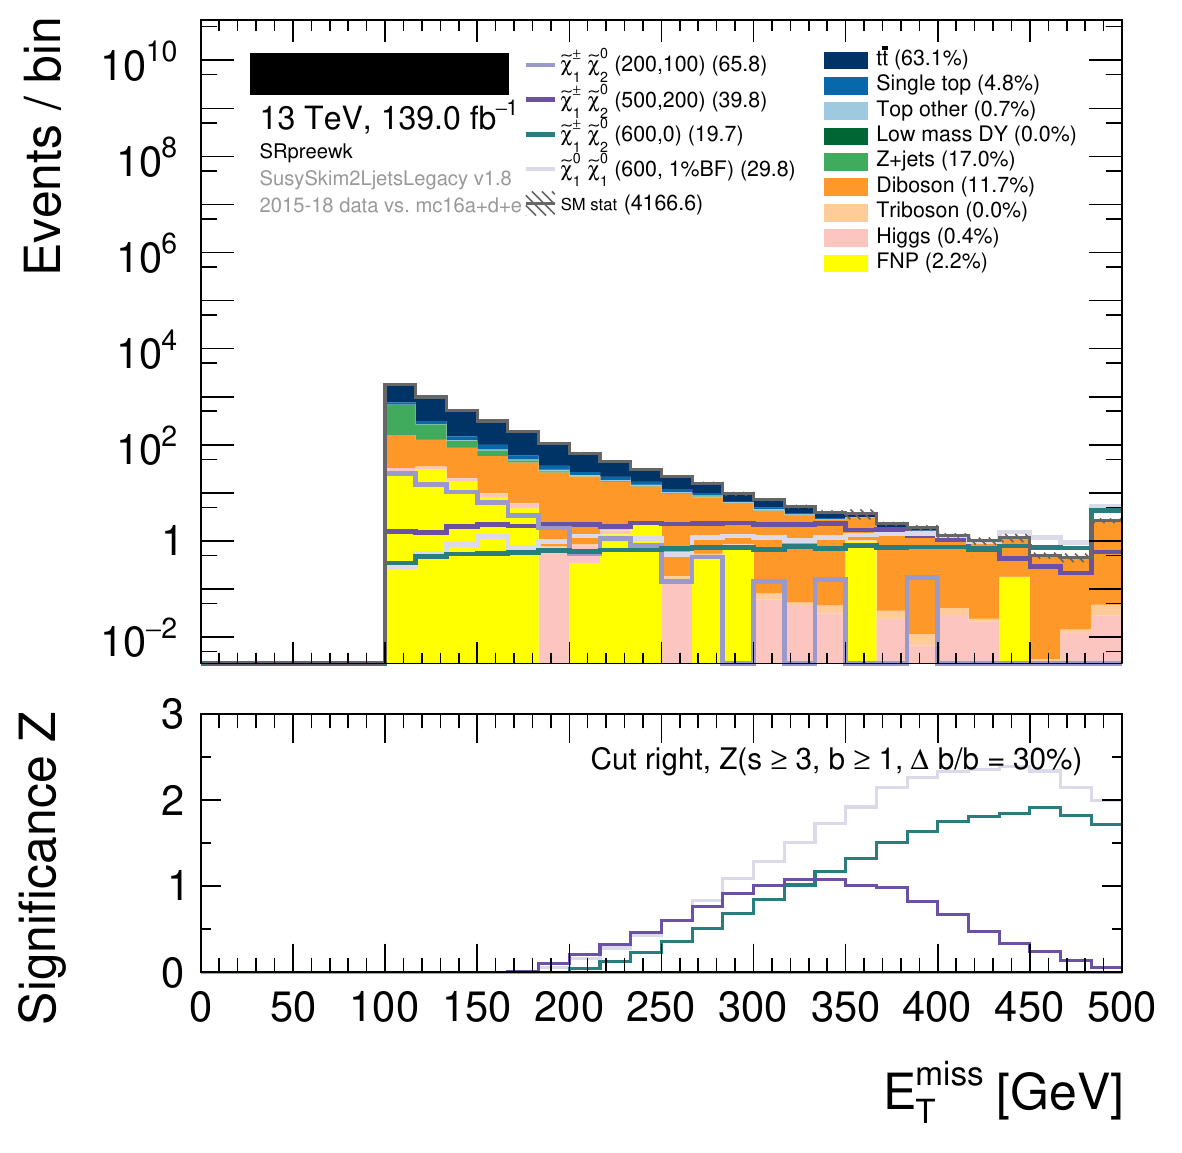
\includegraphics[width=0.6\textwidth]{figures/2ljets_presel_met_logy.png}
\\
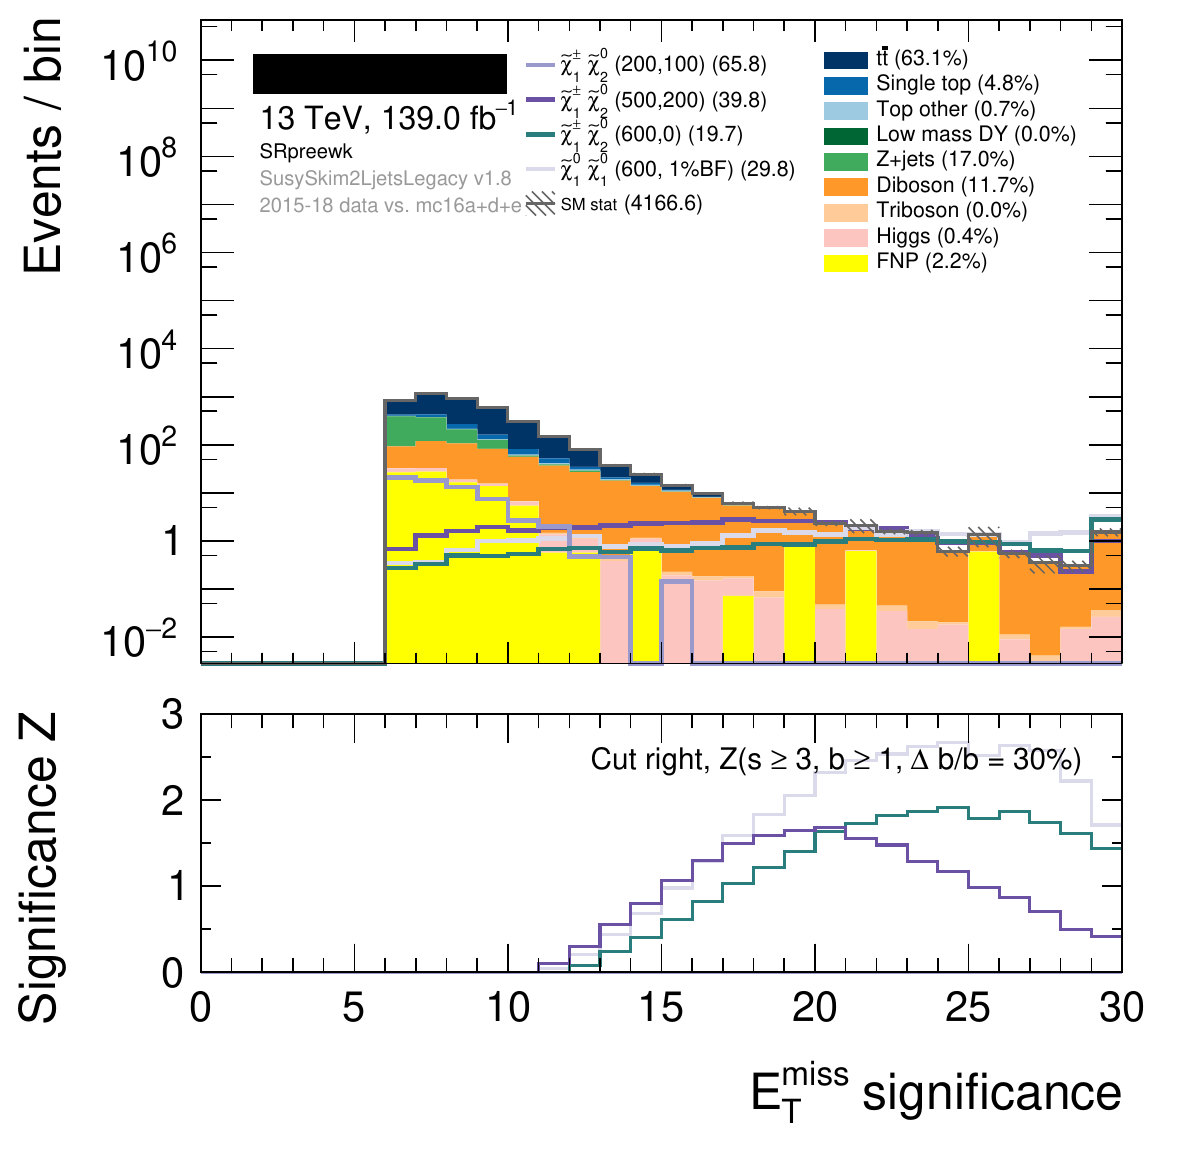
\includegraphics[width=0.6\textwidth]{figures/2ljets_presel_met_sig_logy.png}
\caption[
Illustration of how $\metsig$ beats $\met$ in sensitivity to example signal
models
]{
Illustration of how $\metsig$ beats $\met$ in sensitivity to example signal
models; $\met$ is the missing transverse momentum, and $\metsig$ is its
significance as defined in Section~\ref{sec:2ljets_metsig}.
At large $\metsig$, $\ttbar$ and other backgrounds are suppressed, leaving
quite pure \diboson\ backgrounds and greater significance measures.
Signal models with smaller mass-splittings tend to have the bulk of their
events at smaller $\met$.
\\
This selection requires two same-flavour opposite-sign signal leptons with
$\pt^{\ell_2} > 25\,\eV[G]$,
$\mll \in 71\textrm{--}111\,\eV[G]$,
$\mjj \in 60\textrm{--}110\,\eV[G]$,
$\nbtag \leq 1$,
$\met > 100\,\eV[G]$, and
$\metsig > 6$;
these variables are defined in Section~\ref{sec:2ljets_cheatsheet}.
\\
``Significance'' in the lower plot is
$Z_{Bi}$ from~\cite{cousins2008evaluation}, with a $30\%$ uncertainty and
yields taken to the right of a given value.
}
\label{fig:2ljets_presel_met}
\end{figure}

Uncertainty in $\ptmiss$ is modelled for $\metsig$ by a covariance matrix
$\Sigma$ in the transverse plane, and used to define
\begin{equation}
\metsig^2
=
\ptmiss\,{}^T \Sigma^{-1} \ptmiss
=
\frac{(\met)^2}{\sigma_L^2(1 - \rho_{LT}^2)}
,
\end{equation}
in which $\sigma_L^2$ is the variance in the direction of $\ptmiss$ and
$\rho_{LT}$ is the correlation coefficient between the parallel and
perpendicular components~\cite{atlas_met_significance}.
This is a squared `Mahalanobis' (standard-deviations)
distance~\cite{mahalanobis1936generalised} between $\ptmiss$ and the origin.

Just as $\ptmiss$ is constructed from a (negative) sum of contributions from
objects in an event, this $\Sigma$ is a sum of covariance matrices assigned to
those objects; both means and variances add linearly.


\subsection{\texorpdfstring{$\mttwo$}{mT2}}
\label{sec:2ljets_mt2}
Just as the slepton is a supersymmetric partner to a lepton, the `stransverse'
mass $\mttwo$ is a partner to the `transverse mass' $m_T$
(to be defined shortly),
which is useful in searches for supersymmetric particles.

The stransverse mass of an event is a greatest lower bound on the mass of a
pair-produced resonance that applies when each partner decays semi-invisibly.
For example, an on-shell $\tilde\ell^+\tilde\ell^-$ pair decaying as
$\tilde\ell^+ \to \ell^+ \neutralino_1
,~
\tilde\ell^- \to \ell^- \neutralino_1$ has
$\mttwo(\ell^+, \ell^-, m(\neutralino_1)) \leq m(\tilde\ell)$, plus some error
margin for experimental resolution.
Such cases are common, since R-parity conservation implies pair production,
and the idea that dark matter could comprise the lightest supersymmetric
particle motivates invisible decays.

Lacking direct observation of the sleptons, or any other supersymmetric
resonances, at the LHC, $\mttwo$ remains useful for separating Standard Model
processes since, with ideal reconstruction,
dileptonic $\ttbar$ and $W^\pm W^\mp$ decays both
satisfy $\mttwo(\ell^+, \ell^-, 0) \leq m(W)$ since $m(\nu) \approx 0$.
The $\twoljets$-electroweak search depends on this effect:
most of its selections require $\mttwo(\ell^+, \ell^-, 0) > 80\,\eV[G]$,
or similar,
to reduce $\ttbar$, $W^\pm W^\mp$ and $\tau^\pm\tau^\mp$ backgrounds.

More precisely, the stransverse mass can be defined as
\begin{equation}
\mttwo(a_\mu, b_\mu, m)
=
\min_{\vec p + \vec q=\ptmiss}
\max
\begin{Bmatrix}
m_T(a_\mu + \{\!\sqrt{m^2 + \vec p_T^{\:2}},\,\vec p\,\}_\mu)\\
m_T(b_\mu + \{\!\sqrt{m^2 + \vec q_T^{\:2}},\,\vec q\,\}_\mu)\\
\end{Bmatrix}
,
\end{equation}
in which $m_T^2(p_\mu) = p_0^2 - p_1^2 - p_2^2$ and $\{E,\,\vec p\,\}_\mu$
denotes a four-vector with energy $E$ and momentum
$\vec p$~\cite{lester1999measuring}.
That is, can be seen as exploring the attribution of the observed $\ptmiss$
between the two visible decay products in an event, finding a best mass over
all possible assignments.
As an extension, one can assign different masses $m_p$ and $m_q$ to
the two invisible products~\cite{lester2015bisection}.

Numerical evaluation of $\mttwo$ can be performed efficiently with interval
bisection algorithms that seek the least resonance mass for which the
transverse masses allow any compatible assignment that also satisfies
$\vec p + \vec q = \ptmiss$.
Testing this compatibility reduces to testing for the intersection of two
ellipses, one for each transverse
mass~\cite{cheng2008minimal, lester2015bisection}.

Public code for calculating $\mttwo$ is available in a Python
library~\cite{gillam2021mt2}, to which I contributed a faster and more robust
implementation of the bisection algorithm of
Lester and Nachman~\cite{lester2015bisection} during this project.
\emph{Thanks to Tom~Gillam and Christopher~G.~Lester for collaboration on
refining this implementation.}


\subsection{Jet pairs}
In $\twoljets$, di-jet assignments for variables like $\mjj$ and $\rjj$ are
always chosen as the two hardest jets. Why?
One reason is that this choice matches the convention of SR2-int and SR2-high
from the previous search~\cite{atlas_23l_SUSY_2016_24}.
However, my initial reaction was that since we are looking for jet pairs near
to $m(W)$ or $m(Z)$, we should surely choose candidate jet pairs by their mass.

Two alternative di-jet assignments were therefore considered in early
development of my $\twoljets$-electroweak region designs:
the two jets with invariant mass closest to $m(W)$, and the two jets with the
minimum $\rjj^\mathrm{alternative}$ between them.
The result was bland.
All assignments performed similarly, and all left similar amounts of signal
outside their selected mass windows.
The simplicity of, and precedent for, the two-hardest jet assignment therefore
swung the decision in its favour.

However, alternative jet pair assignments did select different subsets of
signal yields:
the alternative jet assignments had some potential to define secondary signal
regions to catch those signal events that fall outside the primary
$\mjj$ window.
One can, for example, select $\mjj \notin 60\textrm{--}110\,\eV[G]$ and
$\mjj^\mathrm{alternative} \in 60\textrm{--}110\,\eV[G]$ for some additional
sensitivity.
However, this comes at the cost of complexity, particularly in the boundaries
with control and validation regions, and is therefore not used here.


\subsection{Cheat-sheet}
\label{sec:2ljets_cheatsheet}
Uncomfortably many event variables are used to define the regions of this
analysis.
For future reference, their meanings, definitions, and references for these
variables are all collected here.
All dimensionful quantities are always reported in $\eV[G]$ units in this
thesis.
This list is roughly sorted to have the most important variables at the top.
\begin{itemize}
\item $\met$: missing transverse momentum
\item $\metsig$: object-based missing transverse momentum significance,\\
described in Section~\ref{sec:2ljets_metsig}
\item $\ptjone$: transverse momentum of the hardest jet%
\vspace{0.4em}
\item $\mll$: invariant mass of the hardest two leptons
\item $\mjj$: invariant mass of the two hardest jets
\item $\mbb$: invariant mass of the two hardest $b$-tagged jets
\item $\mjetone$: mass of the hardest jet
\item $\mttwoll$: `stransverse' mass of the lepton pair with massless
invisibles,\\
described in Section~\ref{sec:2ljets_mt2}
\vspace{0.4em}
\item $\rll$: distance in $\eta\textrm{--}\phi$ between the lepton pair
\item $\rjj$: distance in $\eta\textrm{--}\phi$ between the two hardest jets%
\vspace{0.4em}
\item $\njet$: number of signal jets
\item $\nbtag$: number of b-tagged jets,
described in Section~\ref{sec:2ljets_btagging}
\vspace{0.4em}
\item $\dphillmet$: azimuthal angle between $\vec p_{\ell\ell}$ and $\ptmiss$,
where $\vec p_{\ell\ell}$ is the vector sum of the momenta of the leptons in
the lepton pair.
\item $\dphijmet$: azimuthal angle between the hardest jet and $\ptmiss$
\end{itemize}
All of these are physical properties of particles or collections of particles
that are reconstructed from data.
Note, however, that these are not identical to the same quantities that could
be defined from hypothetically true states of those particles ---
the reconstruction for a given `truth' state can vary with noise.
While I admit to dropping this distinction in lax language, it is needed to
explain the broad shapes of noisy variables such as $\mjj$ and indeed the
existence of $\metsig$, which relies on estimates of the reconstruction noise
and is ill-defined at a particle-truth level.

Broadly speaking, some of these variables select necessary conditions for
signal-like events, and others help to improve signal purity within those
selection requirements.
Specifically, our signals produce $\met$, lepton pairs with
$\mll \approx m(Z)$, and jets leading to positive $\njet$.
Requiring appropriate conditions on these variables rejects large
Standard Model background yields without harming signal efficiency.
Other variables help to reduce background contamination with some trade-off
against signal efficiency; among these, $\metsig$ is the most generally strong
separating variable, and other variables are chosen in contexts where
they aid the local designs that we detail in Section~\ref{sec:2ljets_design}.


\FloatBarrier
\section{Design}
\label{sec:2ljets_design}
Perhaps the most impactful decision in an \atlas\ SUSY search is the design of
its regions.
Like most decisions, these designs must be made to balance conflicting and
vaguely-specified desires, and are informed with incomplete information.

In my understanding of search design, there is a deep conflict between
simplicity and precision.
Yes, an extra bin with higher $\metsig$ might catch some extreme signals,
and yes, an RJR construction might pick out candidate decay trees without
extreme $\met$.
But if these delay our result without comparable benefits, they will act to
slow down scientific progress in the area.

Furthermore, simplicity encourages interpretability and trust.
A selection at $100\,\eV[G]$ may be slightly outperformed in precision by one
at $100.314\,\eV[G]$, but the former is preferable --- it is easily
communicated and perhaps understood or reproduced by readers.
The latter could be overly tuned, perhaps by a learning algorithm, to specific
simulations; perhaps it cut out a highly weighted sample that, although
annoying, was an
honest representation of our modelling.
Restricting ourselves to round numbers (in the units with which we communicate)
not only clarifies our communications,
but keeps us honest by restricting our ability to over-fit to simulations.

Numerical simplicity is valuable.
In a draft of our \atlas-internal documentation, I wrote that numerical
simplicity was a design goal, but am guilty of removing that statement after a
reviewer suggested that it was ``too honest''.

The remainder of this section describes the designs of the control,
validation, and signal regions of the $\twoljets$ analysis, along with some
reasoning behind those designs.

\begin{figure}[tp]
\centering
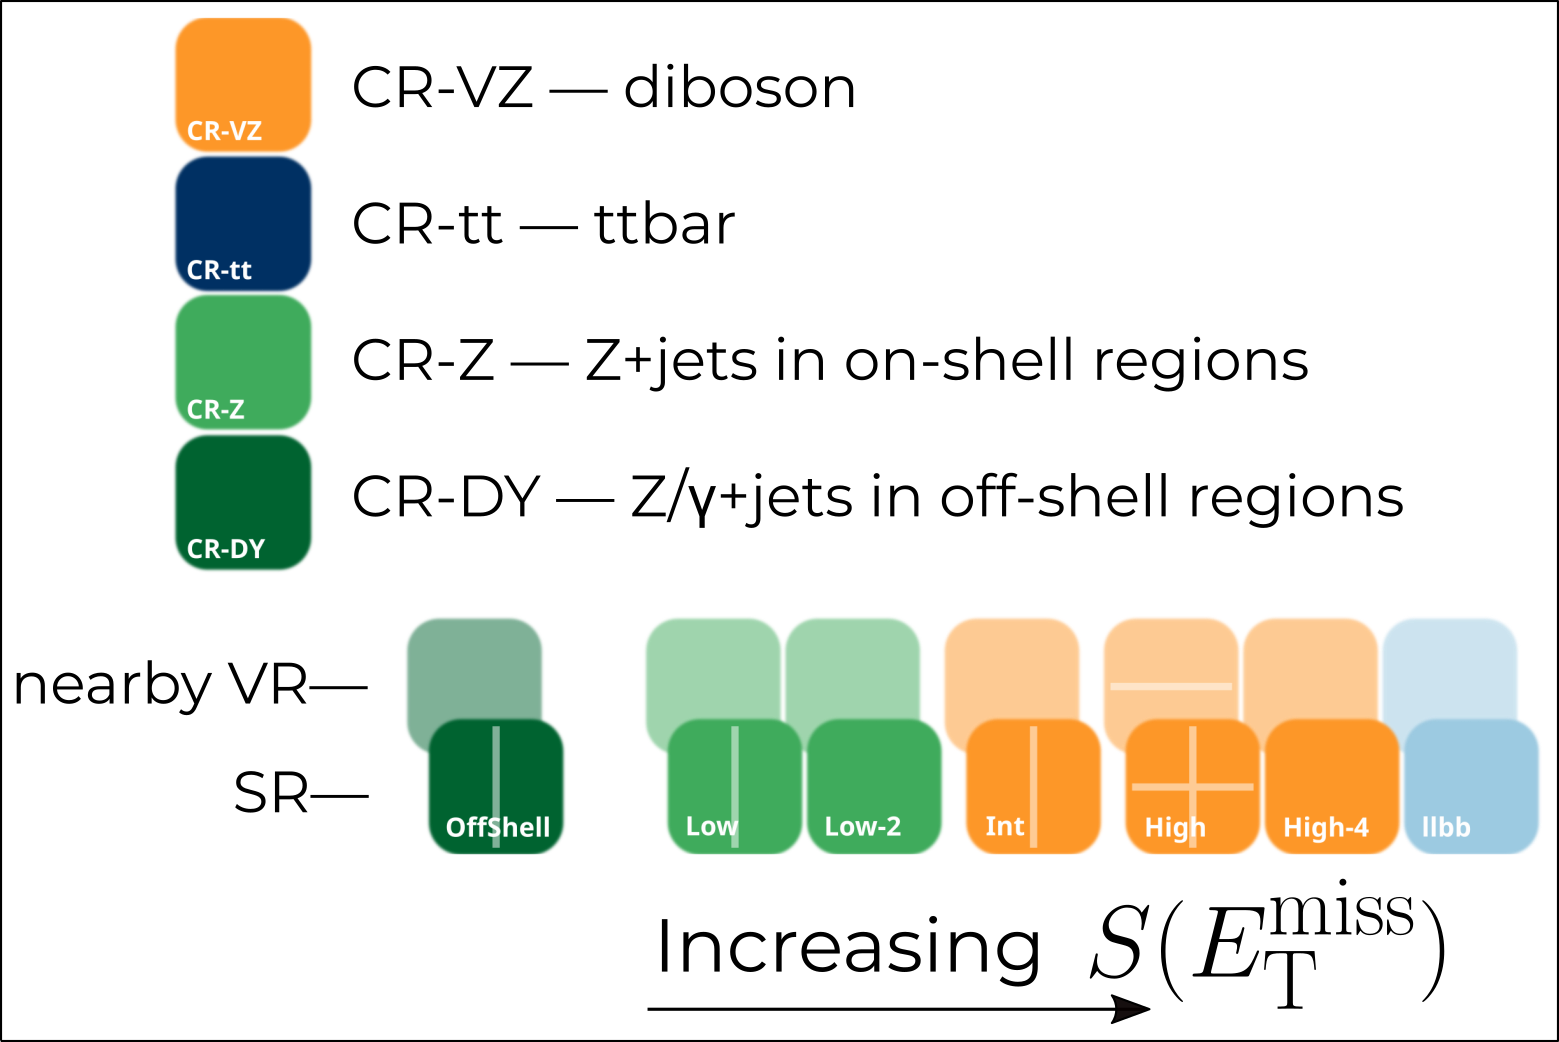
\includegraphics[width=0.99\textwidth]{figures/2Ljets_pam_ewkslide.png}
\caption[
Region design summary slide
]{%
Region design summary slide adapted from an internal presentation.
Colours represent primary background contributions in our plotting scheme.
}
\label{fig:2ljets_region_summary}
\end{figure}

The first idea behind this design is to split regions on $\metsig$, as
motivated by the histograms displayed in Figure~\ref{fig:2ljets_presel_met};
$\metsig$ does better than $\met$ in separating background and signal
contributions for models with various mass splittings.
Furthermore, $\metsig$ also works to separate signal models from each other:
signals with larger mass differences in their decays to invisibles tend to have
larger $\metsig$.
Initial binning in $\metsig$ therefore offers improved sensitivity to
various parameter points.
In each $\metsig$ bin, the $\twoljets$-electroweak design further targets
signal sensitivity with other, locally-relevant event variables.

Three of our signal $\metsig$ bins are named
`High',
`Intermediate' (or `Int'), and
`Low',
to label both the size of $\metsig$ they require and the size of
mass-splittings they target.
These High, Int, and Low selections all target lepton pairs on the $Z$
resonance mass.
Separate `OffShell' regions target $\mll < m(Z)$ events that arise
in models with small mass splittings that force decays to proceed via
low-mass off-shell weak bosons.

Following the conventional style described in
Section~\ref{sec:searches_searches},
control regions are defined to normalize specific background samples,
and validation regions are defined to test their extrapolation towards
signal regions before unblinding.

All $\twoljets$-electroweak regions are defined within a loose `Pre-selection'
requirement of the basic $Z\to \ell\ell$ plus jets plus $\met$
conditions that we target.
These Pre-selection requirements are defined in Table~\ref{tab:2ljets_presel}.

\begin{table}[tp]
\centering
\begin{tabular}{c}
Pre-selection:
\\[1em]
$n_\mathrm{leptons}^\mathrm{signal} = n_\mathrm{leptons}^\mathrm{baseline} = 2$,
\\[0.4em]
same flavour, opposite charge leptons,
\\[0.4em]
$\njet \geq 1$,
\\[0.4em]
$p_\mathrm{T}^{\,\ell_2} > 25$,
\\[0.4em]
\hphantom{~and}$\metsig > 6$, and
\\[0.4em]
$\met > 100$.
\end{tabular}
\caption[%
Pre-selection requirements ensured prior to all region definitions in the
$\twoljets$-electroweak search
]{%
Pre-selection requirements ensured prior to all region definitions in the
$\twoljets$-electroweak search.
Although $\metsig > 6$ implies that most events already have large $\met$, the
$\met > 100\,\eV[G]$ requirement is included to exclude any rare events with
small $\met$ and precise reconstructions.
}
\label{tab:2ljets_presel}
\end{table}

In the remainder of this section,
High regions are discussed in Section~\ref{sec:2ljets_high}.
Intermediate regions are discussed in Section~\ref{sec:2ljets_int}.
Low regions are discussed in Section~\ref{sec:2ljets_low}.
Off-shell regions are discussed in Section~\ref{sec:2ljets_high}.
Control and validation regions are included in these sections near to their
targetted regions.
Finally, how these are combined into `Discovery' regions for
model-independent interpretations is discussed in
Section~\ref{sec:2ljets_disco}.

A high-level summary of the region design is shown in
Figure~\ref{fig:2ljets_region_summary}.
The design comprises four control regions and thirteen orthogonal signal region
bins, with validation regions targeting each group of signal regions.

\emph{%
Thanks to Knut~Vadla for important contributions in the initial signal region
designs, to Ben~Hooberman for suggesting the investigation of massive jets,
and to the whole $\twoljets$ team for collaboration in their finalization.%
}


\subsection{High}
\label{sec:2ljets_high}
Our highest $\metsig$ selections, starting around $\metsig > 18$, contain
pure \diboson\ backgrounds in relatively small quantities, along with the bulk
of signal samples at the heaviest resonance masses.
This is therefore the most promising territory for signal regions that are
highly sensitive to the most extreme signals.
Their backgrounds, however, must be constrained by control regions in
less-extreme parameter spaces with sufficiently many data to precisely
normalize their scale factors.

Diboson backgrounds and C1N2 signals have more in common than just $\met$;
both also produce resonant $Z\to \ell\ell$ pairs
and do not enhance the rate of heavy-flavour jets, as displayed in
Figure~\ref{fig:2ljets_high_mll_b}.
Since signals and backgrounds have such similar shapes in $\mll$ and $\nbtag$,
sensitivity is only decreased by rejecting portions of these distributions.
Although most $\twoljets$-electroweak regions use tighter selection on these
variables to reduce backgrounds, this observation allows us to win
additional sensitivity in High regions by loose requirements
of $\mll \in 71\textrm{--}111\,\eV[G]$%
\footnote{%
We use interval notation in which
en-dashes `$a\textrm{--}b$' indicate open intervals $(a, b)$, and
concatenated intervals `$a\textrm{--}b\textrm{--}c$' indicate binning
with boundaries at $a$, $b$, and $c$.
This notation is consistent with the $\twoljets$
paper~\cite{atlas2022searches}.%
}
and $\nbtag \leq 1$.
This $\mll$ window loosely selects the $m(Z)$ peak to scoop up nearby rare or
mismeasured events away from the central peak.
Similarly, allowing up to one $b$-tag improves yields without boosting
backgrounds, since the $\metsig$ requirement already removes most $\ttbar$
processes.

\begin{table}[tp]
\centering
\begin{tabular}{lccccc}
& $\njet$
& $\nbtag$
& $\metsig$
& $m_*$
& $\rjj$
\\[1em]
SR-High
& $\geq2$
& $\leq 1$
& $18\textrm{--}21\textrm{--}\infty$
& $\mjj\!:~  60\textrm{--}110$
& $0\textrm{--}0.8\textrm{--}1.6$
\\[0.4em]
\: VR-High
& $\geq2$
& $\leq 1$
& $> 18$
& $\uwave{\mjj\!:~  20\textrm{--}60 \mid 110\textrm{--}\infty}$
& $< 1.6$
\\[0.4em]
\: VR-High-R
& $\geq 2$
& $\leq 1$
& $> 18$
& $\uwave{\mjj\!:~  > 20}$
& $\uwave{> 1.6}$
\\[1em]
SR-High-1J
& $\hphantom{\geq}~1$
& $\leq 1$
& $> 12$
& $\mjetone\!:~  60\textrm{--}110$
&
\\[0.4em]
\: VR-High-1J
& $\hphantom{\geq}~1$
& $\leq 1$
& $> 12$
& $\uwave{\mjetone\!:~  20\textrm{--}60 \mid 110\textrm{--}\infty}$
&
\\[1em]
\srllbb
& $\geq 2$
& $\geq 2$
& $> 18$
& $\mbb\!:~  60\textrm{--}150$
&
\\[0.4em]
\: VR-$\llbb$
& $\geq 2$
& $\geq 2$
& $\uwave{12\textrm{--}18}$
& $\mbb\!:~  60\textrm{--}150$
&
\end{tabular}
\\[1em]
Common: Pre-selection,
$\mll \in 71\textrm{--}111$, and
$\mttwoll > 80$.
\caption[
High region definitions in the $\twoljets$-electroweak analysis
]{%
High region definitions in the $\twoljets$-electroweak analysis.
En-dashes `$a\textrm{--}b$' indicate open intervals $(a, b)$.
Concatenated intervals `$a\textrm{--}b\textrm{--}c$' indicate binning
with boundaries at $a$, $b$, and $c$.
The mid-bar `$\mid$' indicates logical `or'.
Differences between regions are \uwave{underlined}.
\\[0.4em]
The $\rll$ bins of SR-High are labelled SR-High-8 and SR-High-16, and their
$\metsig$ bins are suffixed -a and -b for $\metsig \in 18\textrm{--}21$
and $\metsig > 21$, respectively.
}
\label{tab:2ljets_high}
\end{table}

\begin{figure}[tp]
\centering
\begin{subfigure}{0.62\textwidth}
\centering
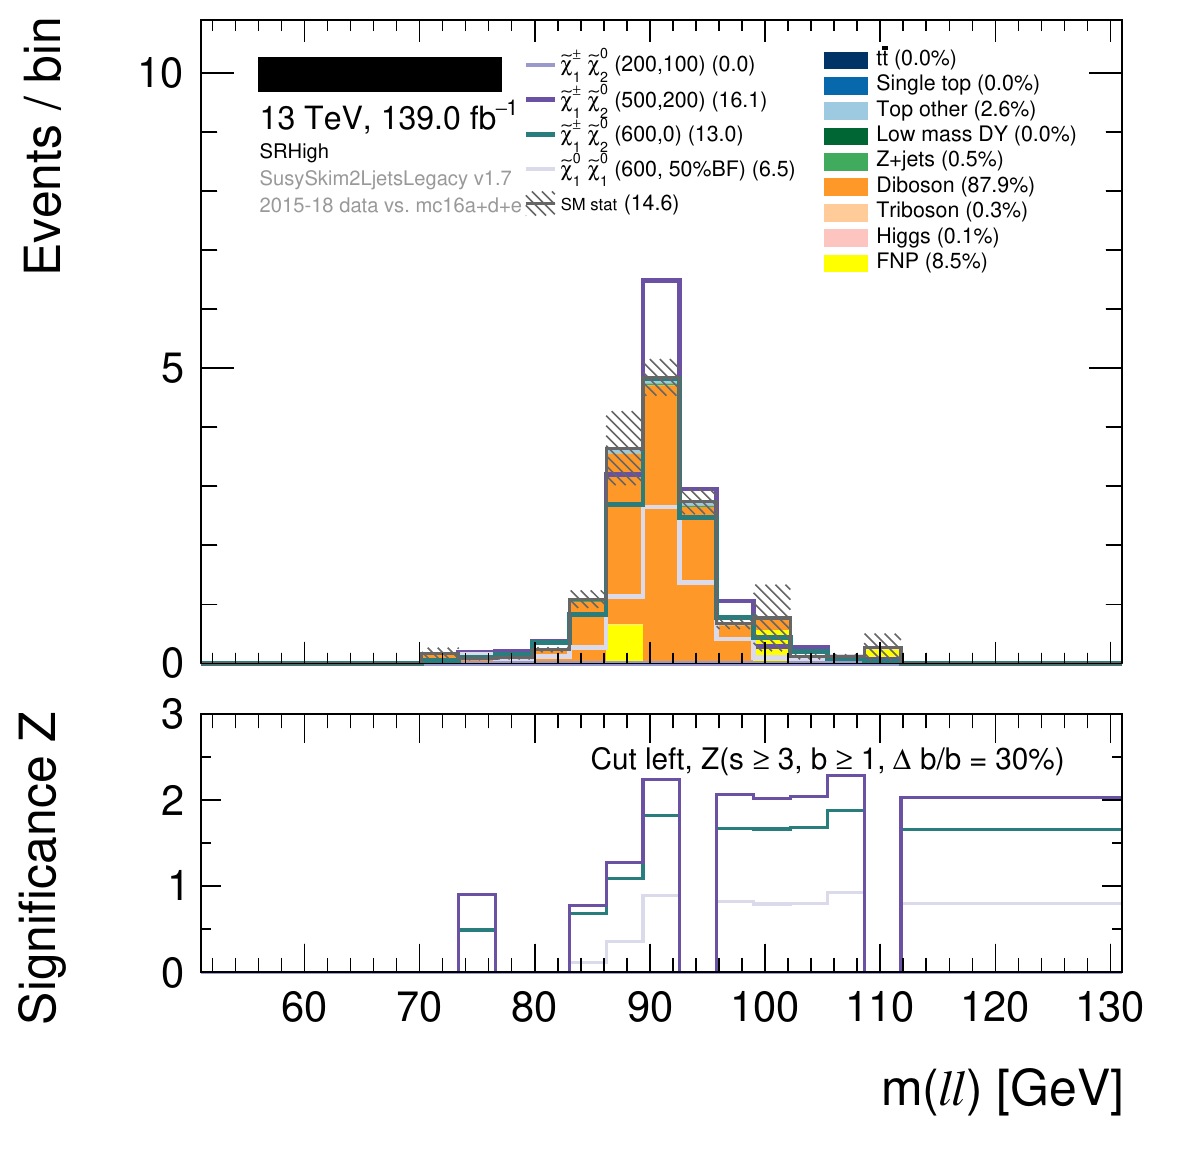
\includegraphics[width=\textwidth]{figures/2ljets_region_design_hist1d_mll_SRHigh.png}
\caption{SR-High, $\mll$}
\end{subfigure}
\\
\begin{subfigure}{0.62\textwidth}
\centering
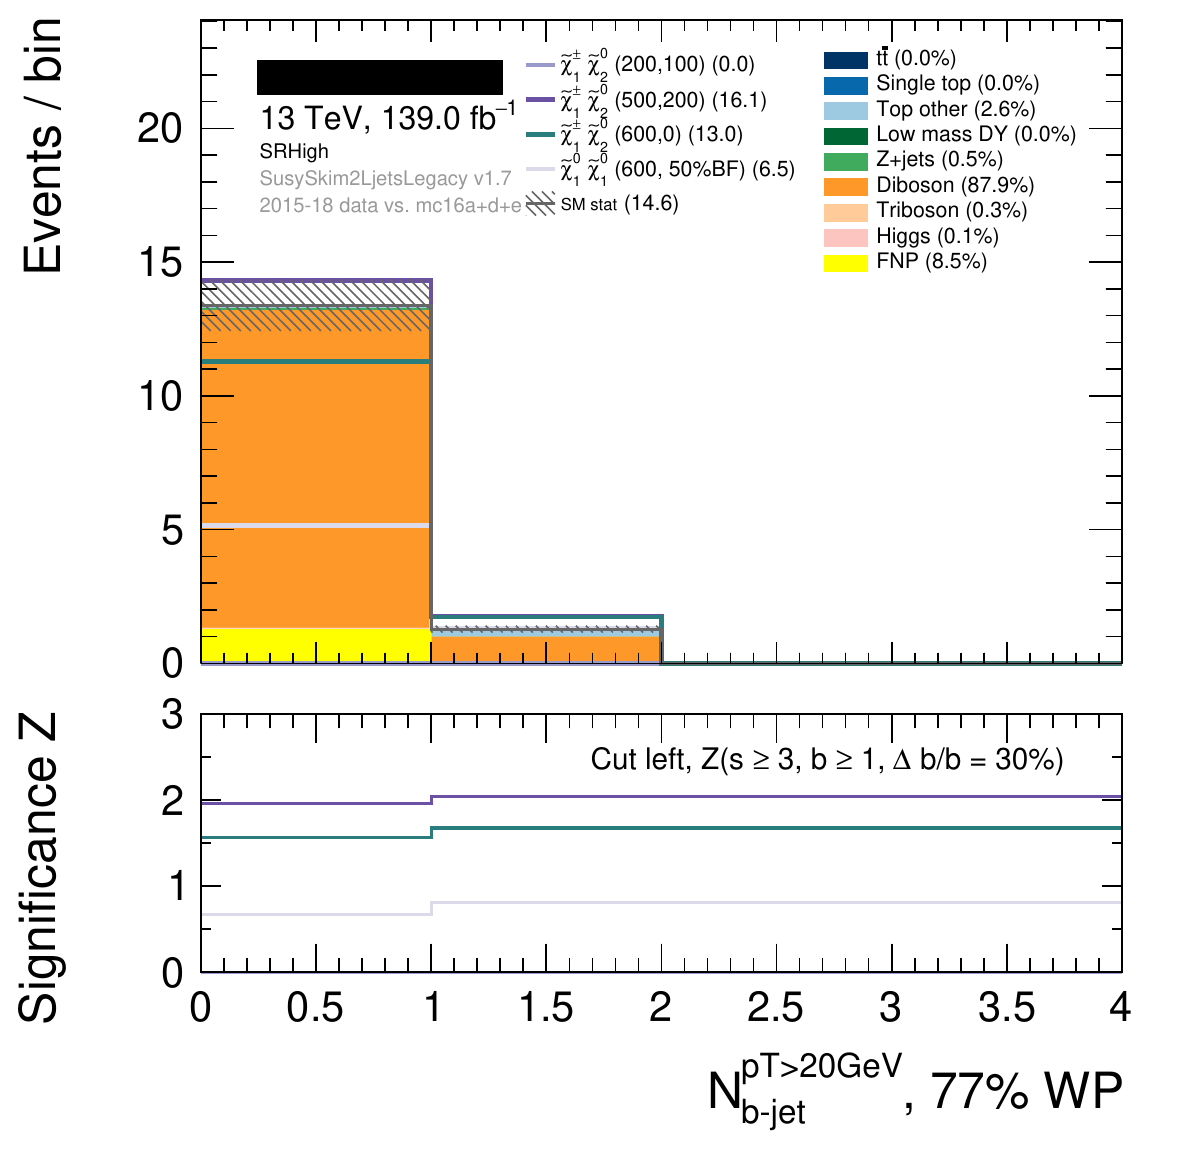
\includegraphics[width=\textwidth]{figures/2ljets_region_design_hist1d_nbtag_SRHigh.png}
\caption{SR-High, $\nbtag$}
\end{subfigure}
\caption[
SR-High with relaxed selections on (a) $\mll$ or (b) $\nbtag$
]{%
SR-High with relaxed selections on (a) $\mll$ or (b) $\nbtag$.
The pure \diboson\ background has very similar shapes to the signals.
Tighter cuts would therefore reduce background and signal yields comparably,
reducing sensitivity.
The significance dropouts in (a) are errors in plotting.
`Significance Z' is the binomial significance~\cite{cousins2008evaluation}
with a $30\%$ relative background uncertainty.
Error bars are statistical.
}
\label{fig:2ljets_high_mll_b}
\end{figure}

The high regions, which are defined in Table~\ref{tab:2ljets_high}, comprise
SR-High, SR-High-1J, and \srllbb.
Their wide standard $\mjj \in 60\textrm{--}110\,\eV[G]$ requirement
captures both $W\to jj$ and $Z\to jj$ for C1N2 and GMSB models,
respectively, and is applied similarly to all other on-shell
$\twoljets$-electroweak signal regions.

As explained in Section~\ref{sec:2ljets_mt2}, requiring $\mttwo$ above $m(W)$
effectively removes $\ttbar$ and other backgrounds.
The relatively low requirement $\mttwoll > 80\,\eV[G]$ is chosen here and
elsewhere in the $\twoljets$-electroweak design to reduce these backgrounds
while minimizing lost signal yields.

To maximize our projected sensitivity, SR-High is split into four bins with
one division at $\rjj = 0.8$, to form SR-High-8 and SR-High-16, and a second
division at $\metsig = 21$ to split each of those into
SR-High-*-a and SR-High-*-b.
For example, SR-High-8-b requires $\rjj < 0.8$ and $\metsig > 21$.
The regions SR-High-8 and SR-High-16 are displayed in
Figure~\ref{fig:2ljets_high_region}, with their -a and -b bins visible across
the $\metsig$ distribution.

\begin{figure}[tp]
\centering
\begin{subfigure}{0.495\textwidth}
\centering
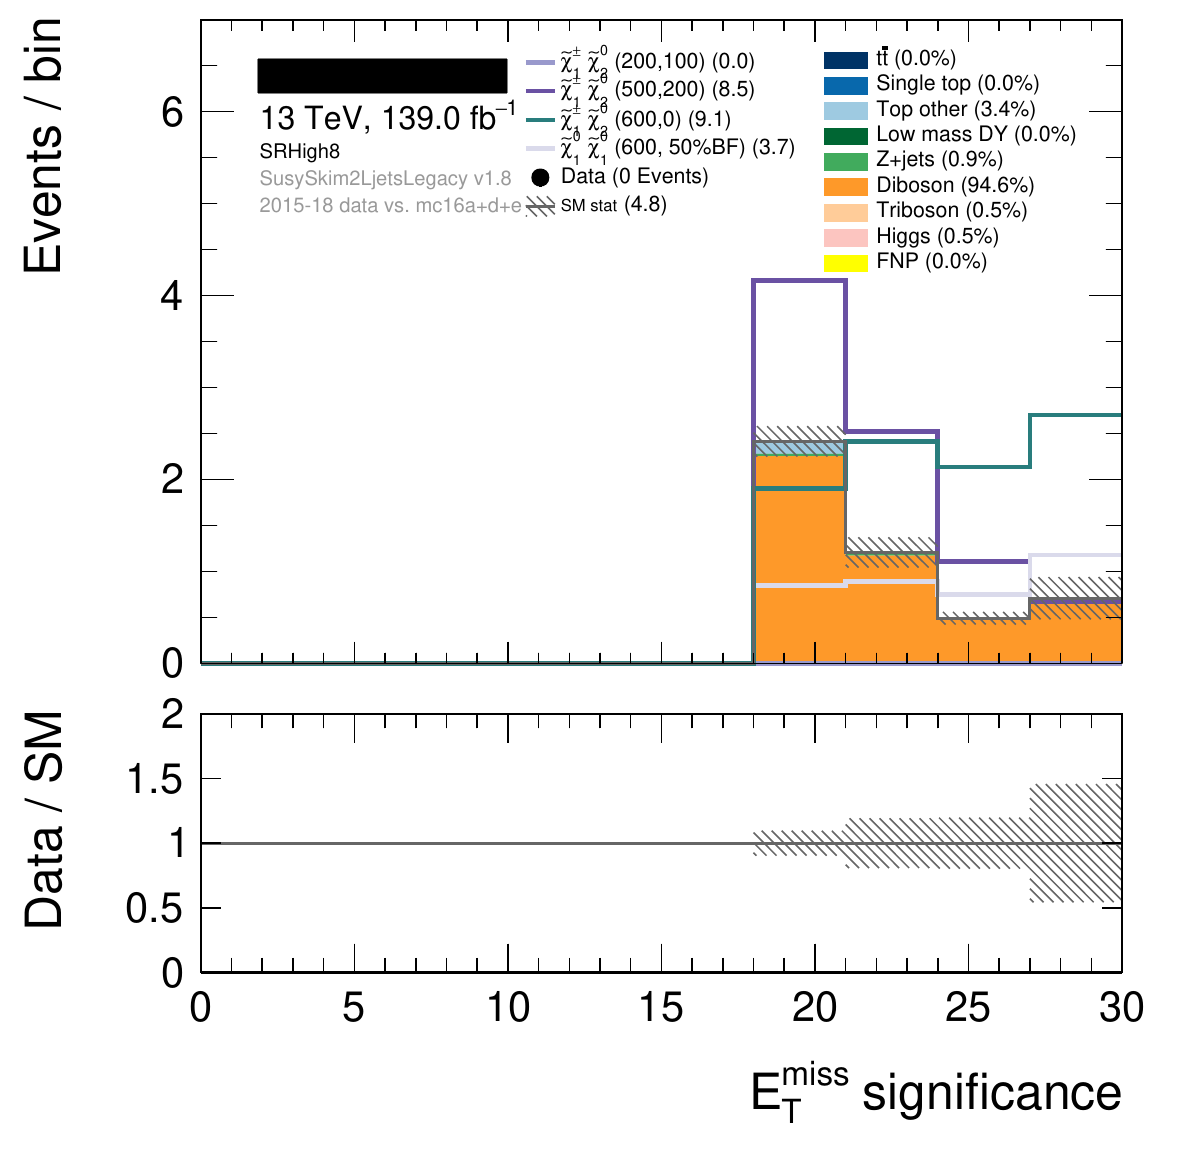
\includegraphics[width=\textwidth]{figures/2ljets_def_met_Sign_SRHigh8.png}
\caption{SR-High-8, $\metsig$}
\end{subfigure}
\hfill
\begin{subfigure}{0.495\textwidth}
\centering
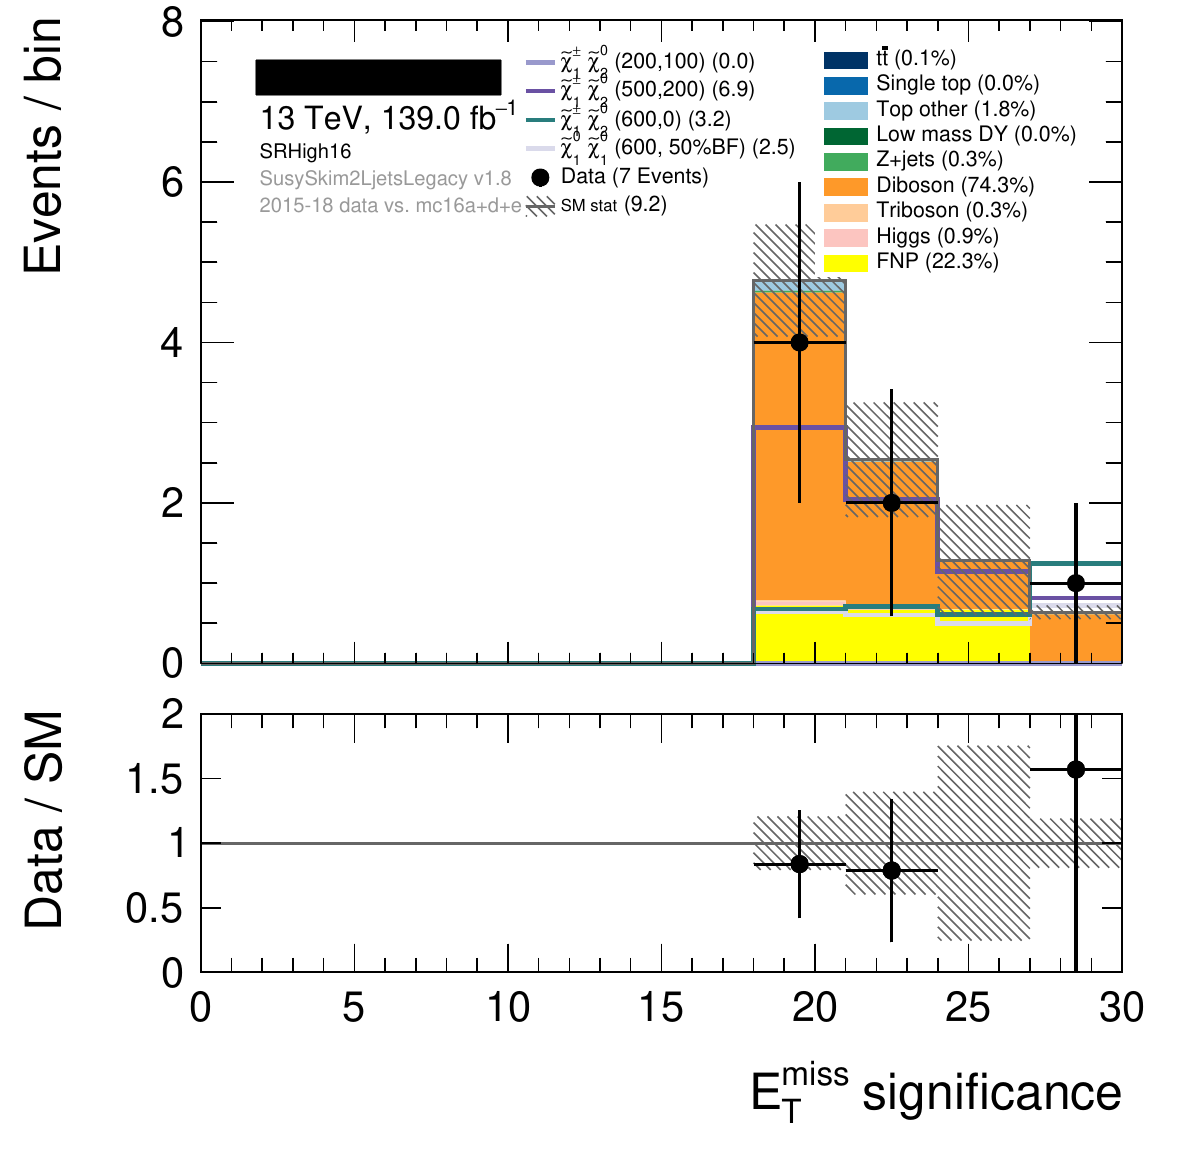
\includegraphics[width=\textwidth]{figures/2ljets_def_met_Sign_SRHigh16.png}
\caption{SR-High-16, $\metsig$}
\end{subfigure}
\\[0.4em]
\begin{subfigure}{0.495\textwidth}
\centering
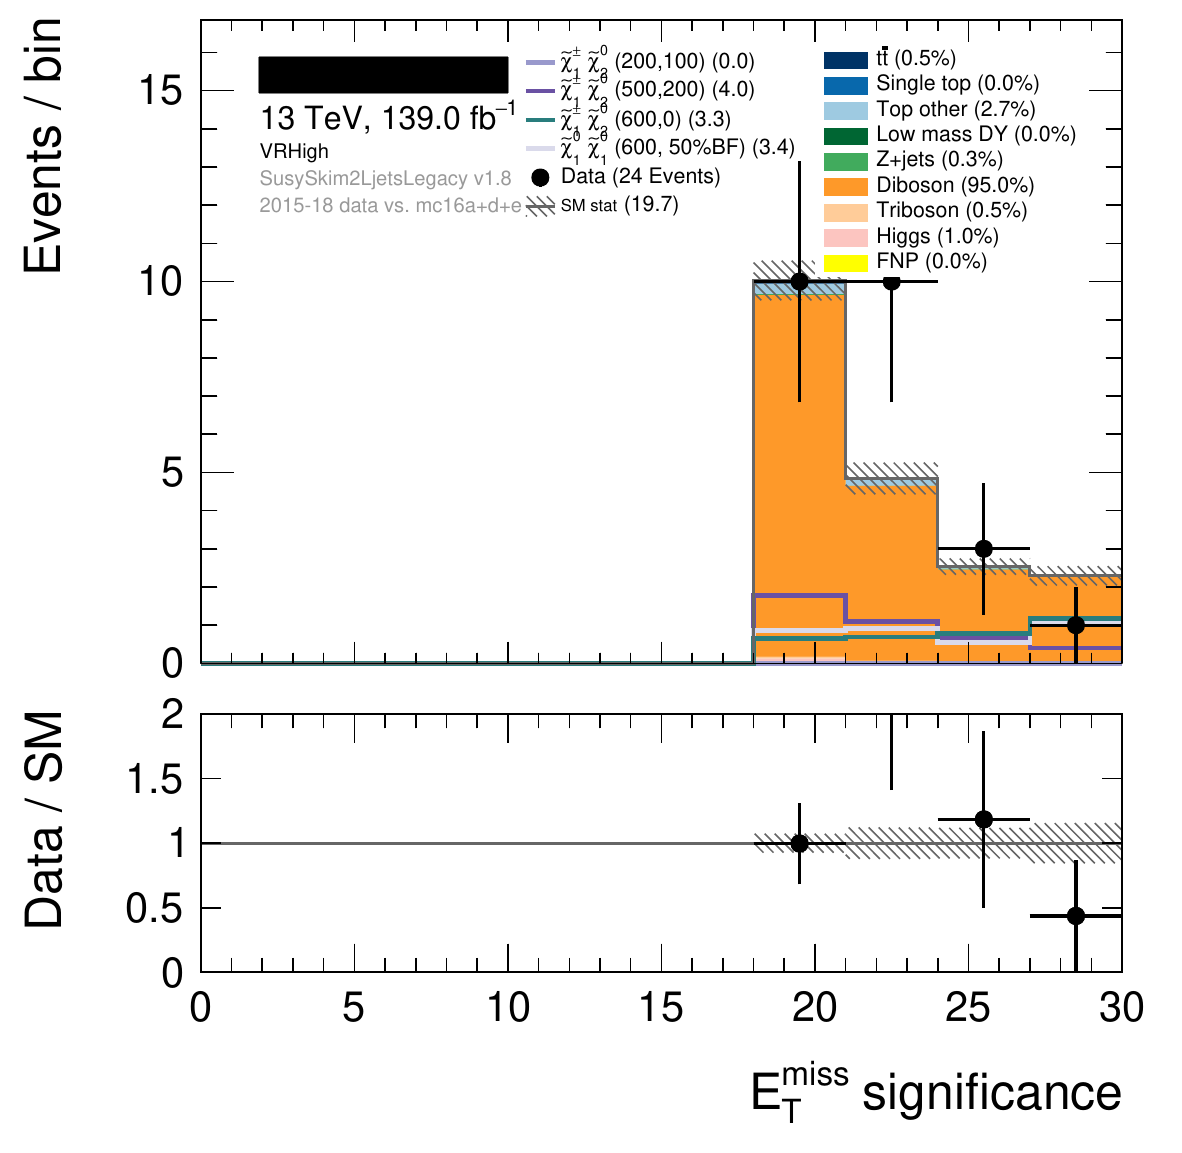
\includegraphics[width=\textwidth]{figures/2ljets_def_met_Sign_VRHigh.png}
\caption{VR-High-8, $\metsig$}
\end{subfigure}
\hfill
\begin{subfigure}{0.495\textwidth}
\centering
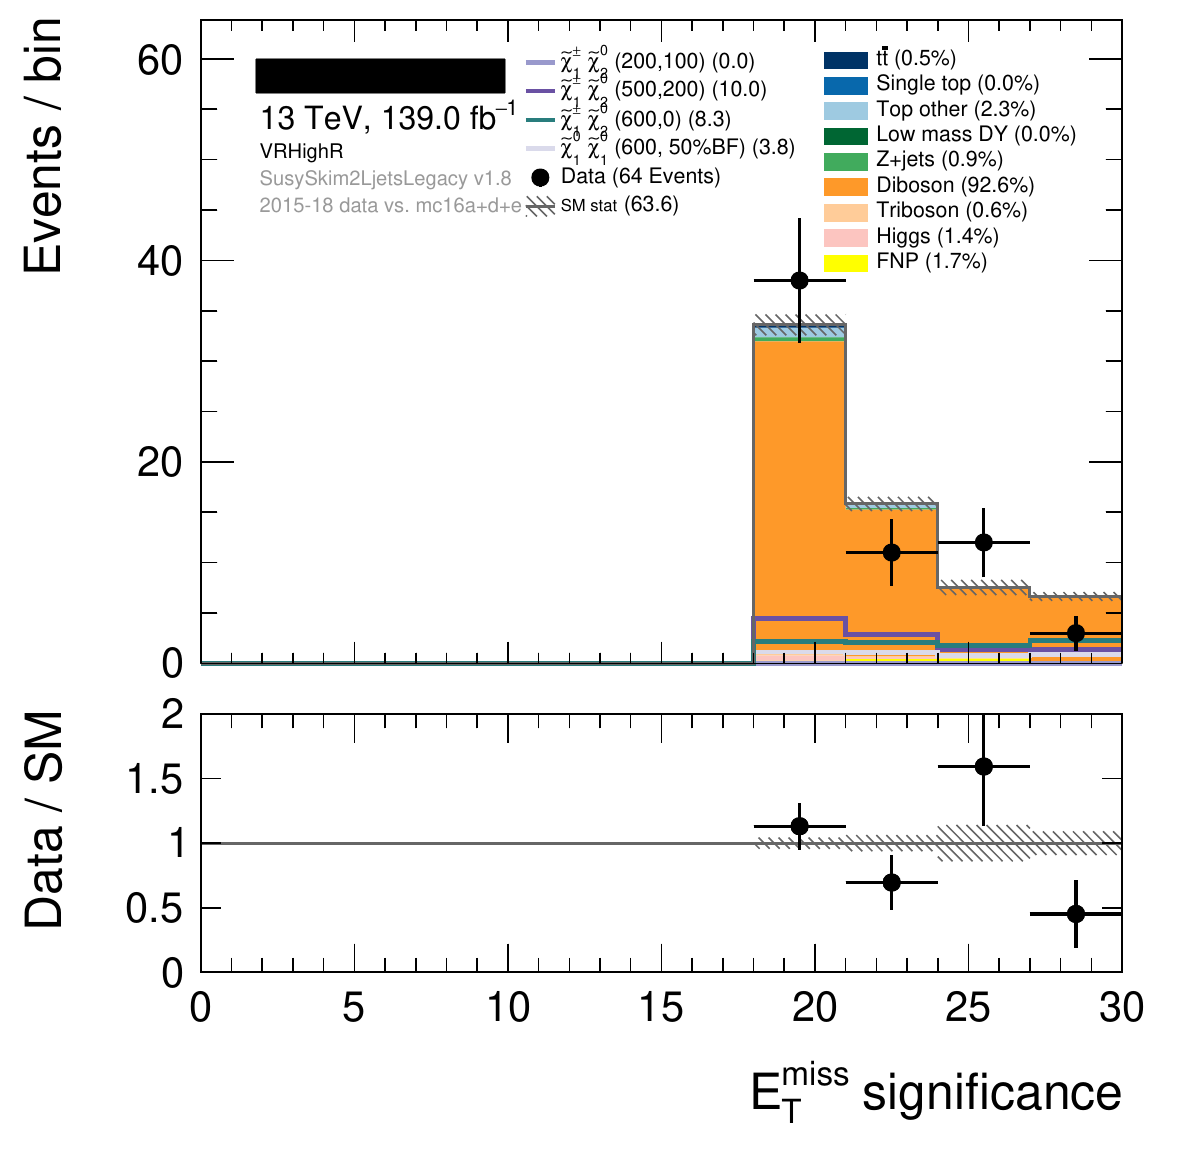
\includegraphics[width=\textwidth]{figures/2ljets_def_met_Sign_VRHighR.png}
\caption{VR-High-16, $\metsig$}
\end{subfigure}
\caption[
Pre-fit distributions of $\metsig$ in High signal and validation regions
]{%
Pre-fit distributions of $\metsig$ in High signal and validation regions.
Signal regions are unblinded.
Errors are statistical.
}
\label{fig:2ljets_high_region}
\end{figure}

One major difference between signals and \diboson\ backgrounds is that signal
jet pairs mostly arise from boosted $W\to jj$ decays, which more often
produce nearby jets.
Selecting small $\rjj$ in SR-High therefore picks out these boosted cases.

Extremely boosted $W$ bosons can be clustered into single jets.
Although large-radius jets are typically used to capture these, we only use
small, $R=0.4$, jets in the $\twoljets$ analysis, and those small jets can
be good enough to work for the extreme boosts that our signals produce.
To catch these extreme events is the goal of SR-High-1J, which is displayed
in Figure~\ref{fig:2ljets_high_1J_region}.
The use of $\mjetone$ with small-radius jets for this region is unusual,
and required modelling of additional uncertainties that we discuss later in
Section~\ref{sec:2ljets_jet_mass}.

\begin{figure}[tp]
\centering
\begin{subfigure}{0.495\textwidth}
\centering
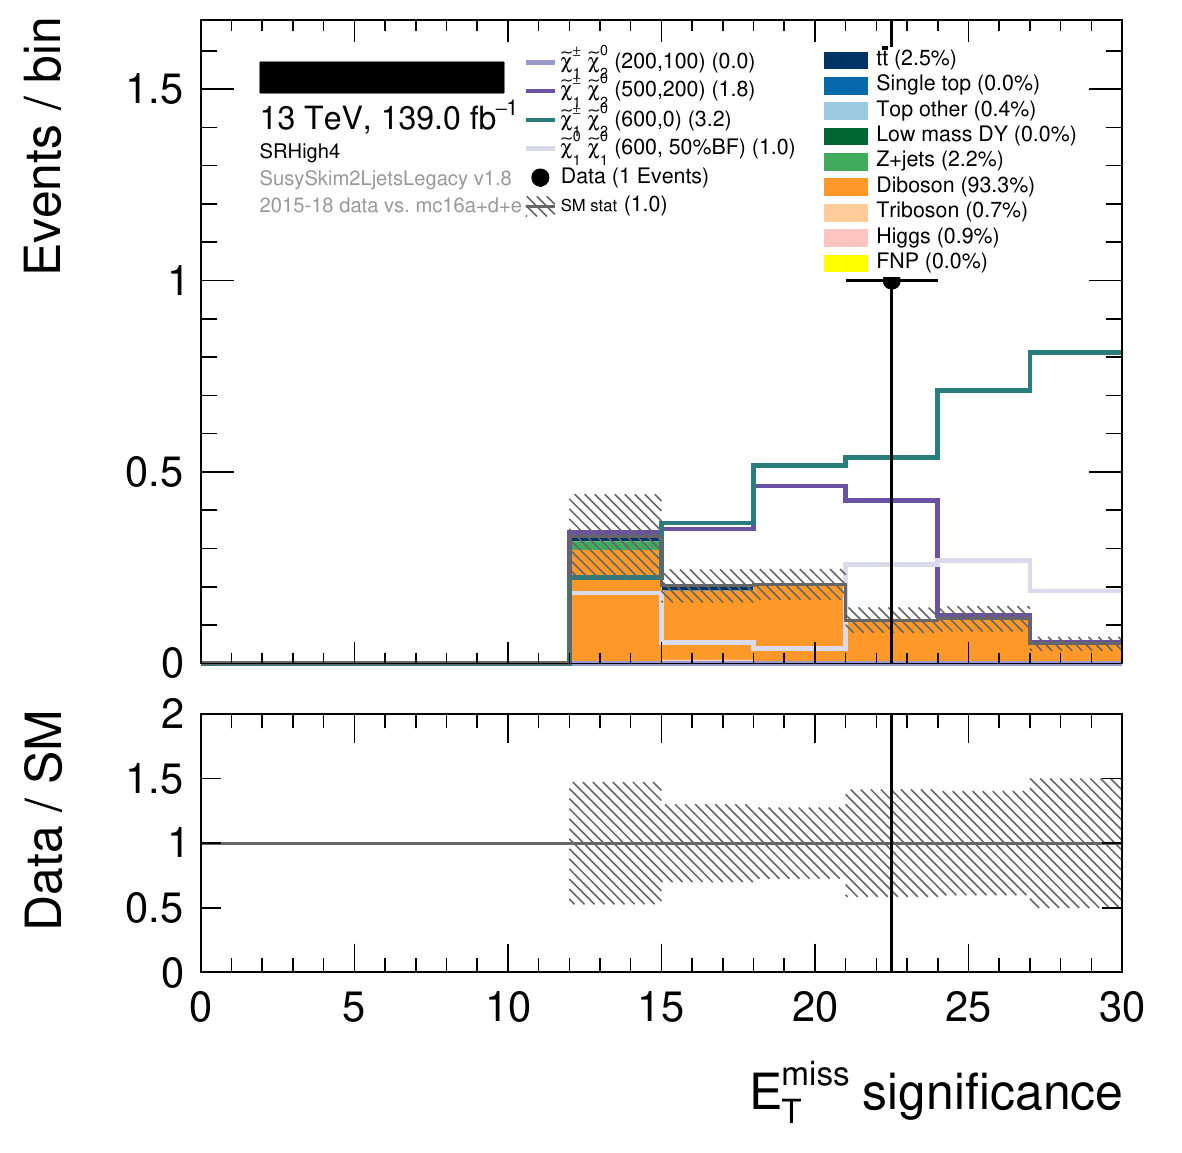
\includegraphics[width=\textwidth]{figures/2ljets_def_met_Sign_SRHigh4.png}
\caption{SR-High-1J, $\metsig$}
\end{subfigure}
\hfill
\begin{subfigure}{0.495\textwidth}
\centering
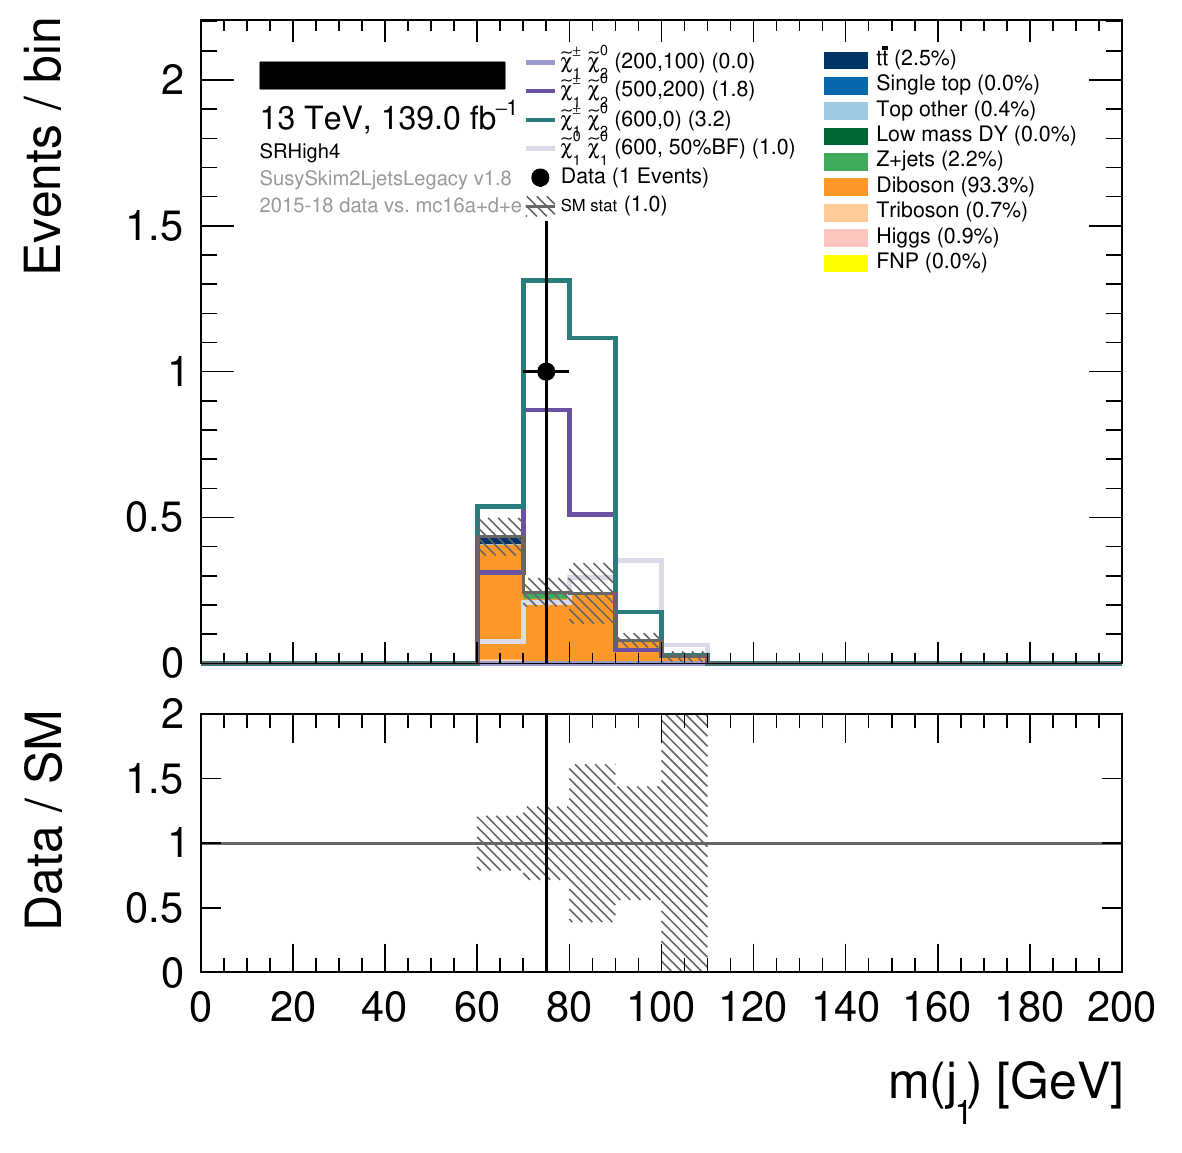
\includegraphics[width=\textwidth]{figures/2ljets_def_mjetone_SRHigh4.png}
\caption{SR-High-1J, $\mjetone$}
\end{subfigure}
\\[0.4em]
\begin{subfigure}{0.495\textwidth}
\centering
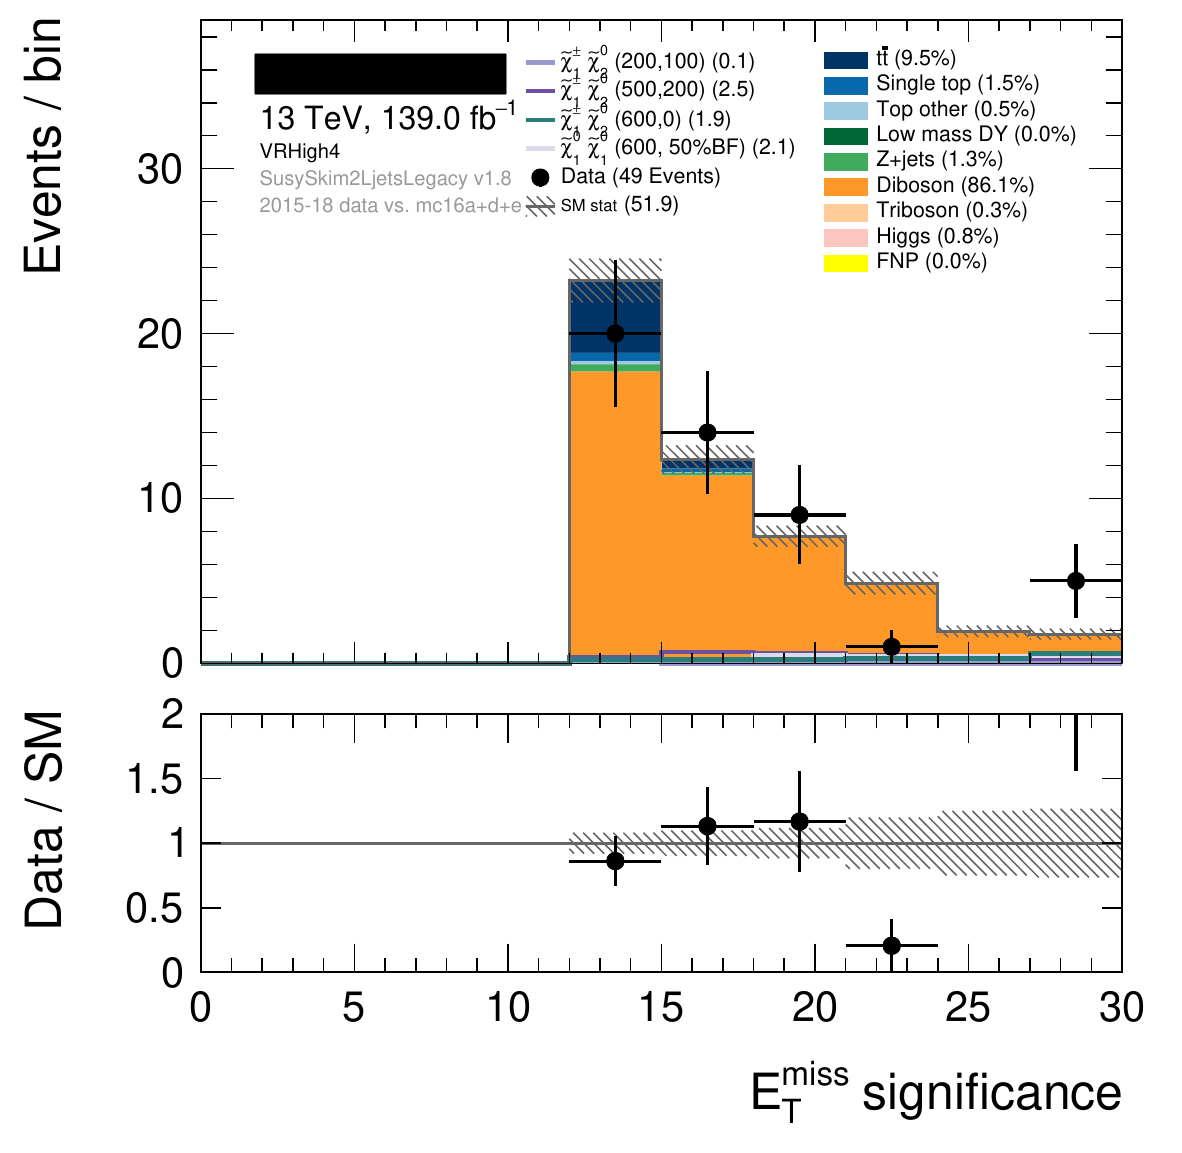
\includegraphics[width=\textwidth]{figures/2ljets_def_met_Sign_VRHigh4.png}
\caption{VR-High-1J, $\metsig$}
\end{subfigure}
\hfill
\begin{subfigure}{0.495\textwidth}
\centering
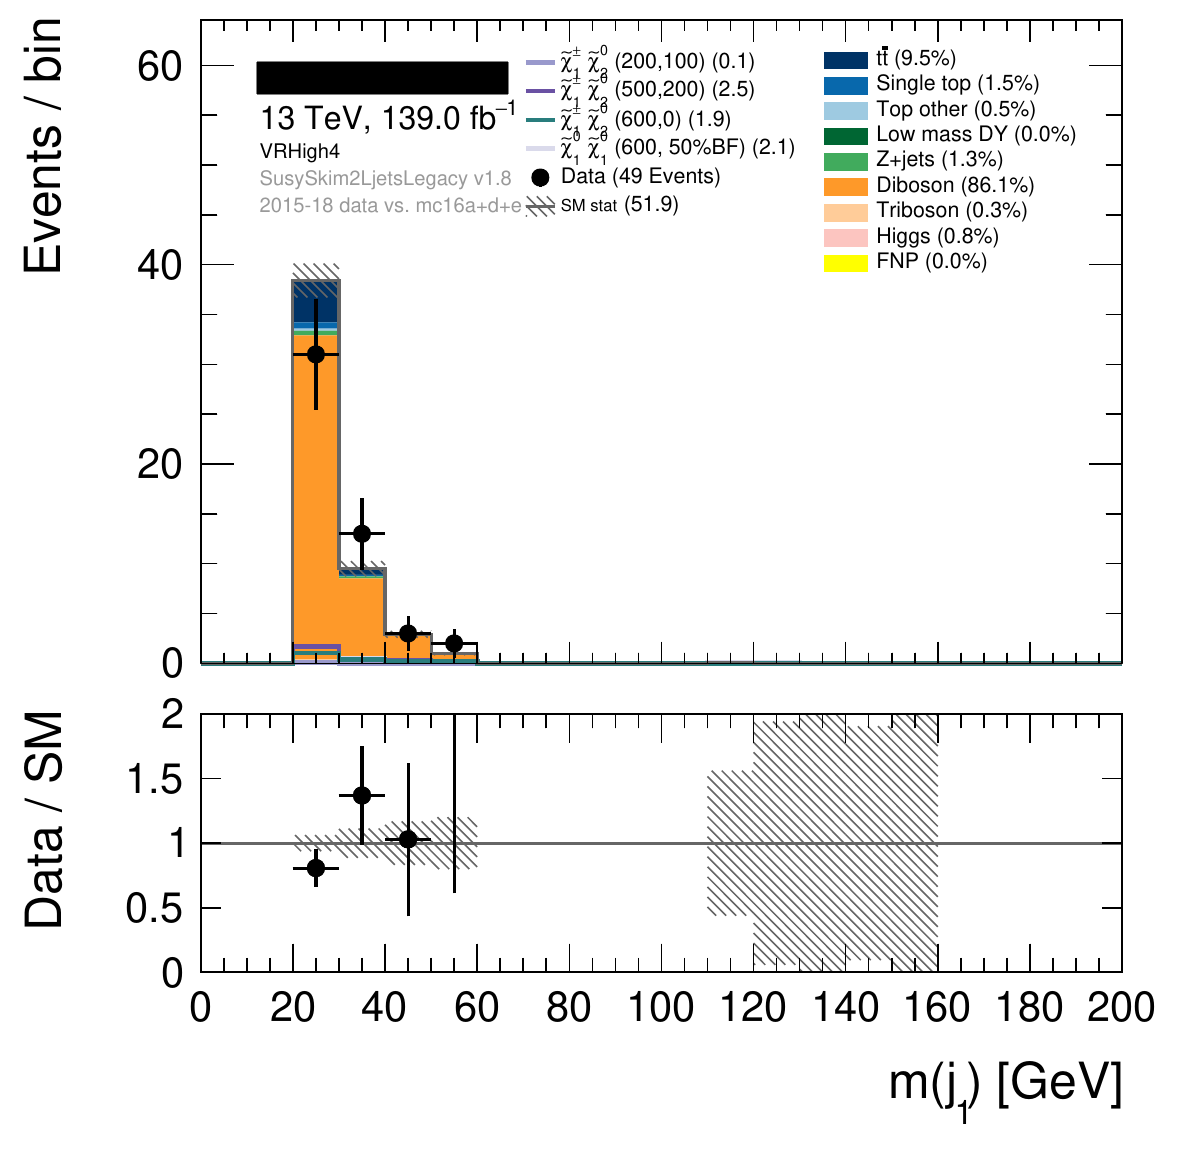
\includegraphics[width=\textwidth]{figures/2ljets_def_mjetone_VRHigh4.png}
\caption{SR-High-1J, $\mjetone$}
\end{subfigure}
\caption[
Pre-fit distributions in mono-jet signal and validation regions
]{%
Pre-fit distributions in mono-jet signal and validation regions.
Signal regions are unblinded.
Errors are statistical.
}
\label{fig:2ljets_high_1J_region}
\end{figure}

All other regions require two jets or more, so this single-jet region design
has the freedom to reduce its $\metsig$ requirement to $\metsig > 12$
without overlapping any other regions.

Finally, \srllbb\ is designed to target the GMSB model, which produces decays
via $ZZ$ and $Zh$ bosons pairs.
Since the $h\to bb$ branching fraction is large, \srllbb\ finds
sensitivity by requiring a pair of $b$-tagged jets in a heavy mass window.
The low edge of this $\mbb \in 60\textrm{--}150\,\eV[G]$ window is far from the
Higgs boson mass at around $125\,\eV[G]$, and is chosen not only to
accommodate \atlas's noisy reconstruction of $b$-jets, but also to
capture $Z\to bb$ decays, which become significant for signal models
with small branching fractions $B(\neutralino_1 \to h \gravitino)$.

As shown in Figure~\ref{fig:2ljets_high_llbb_region}, the Standard Model
background in \srllbb\ contains a significant proportion of \topother\
processes; studies presented in Section~\ref{sec:2ljets_validation} show that
these are mainly $t\bar t Z$.

\begin{figure}[tp]
\centering
\begin{subfigure}{0.495\textwidth}
\centering
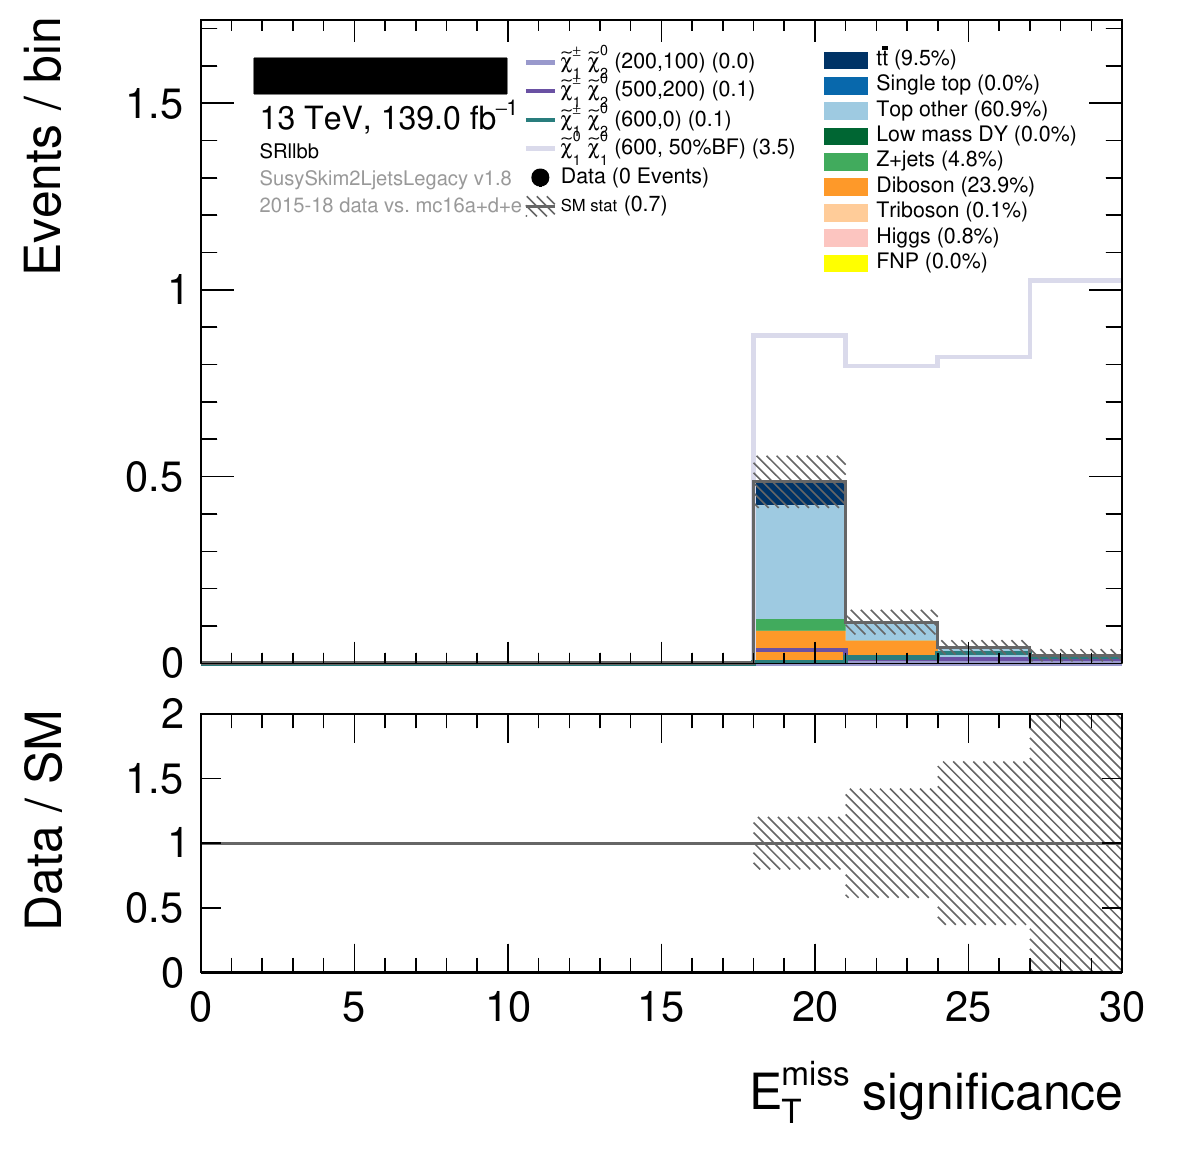
\includegraphics[width=\textwidth]{figures/2ljets_def_met_Sign_SRllbb.png}
\caption{\srllbb, $\metsig$}
\end{subfigure}
\hfill
\begin{subfigure}{0.495\textwidth}
\centering
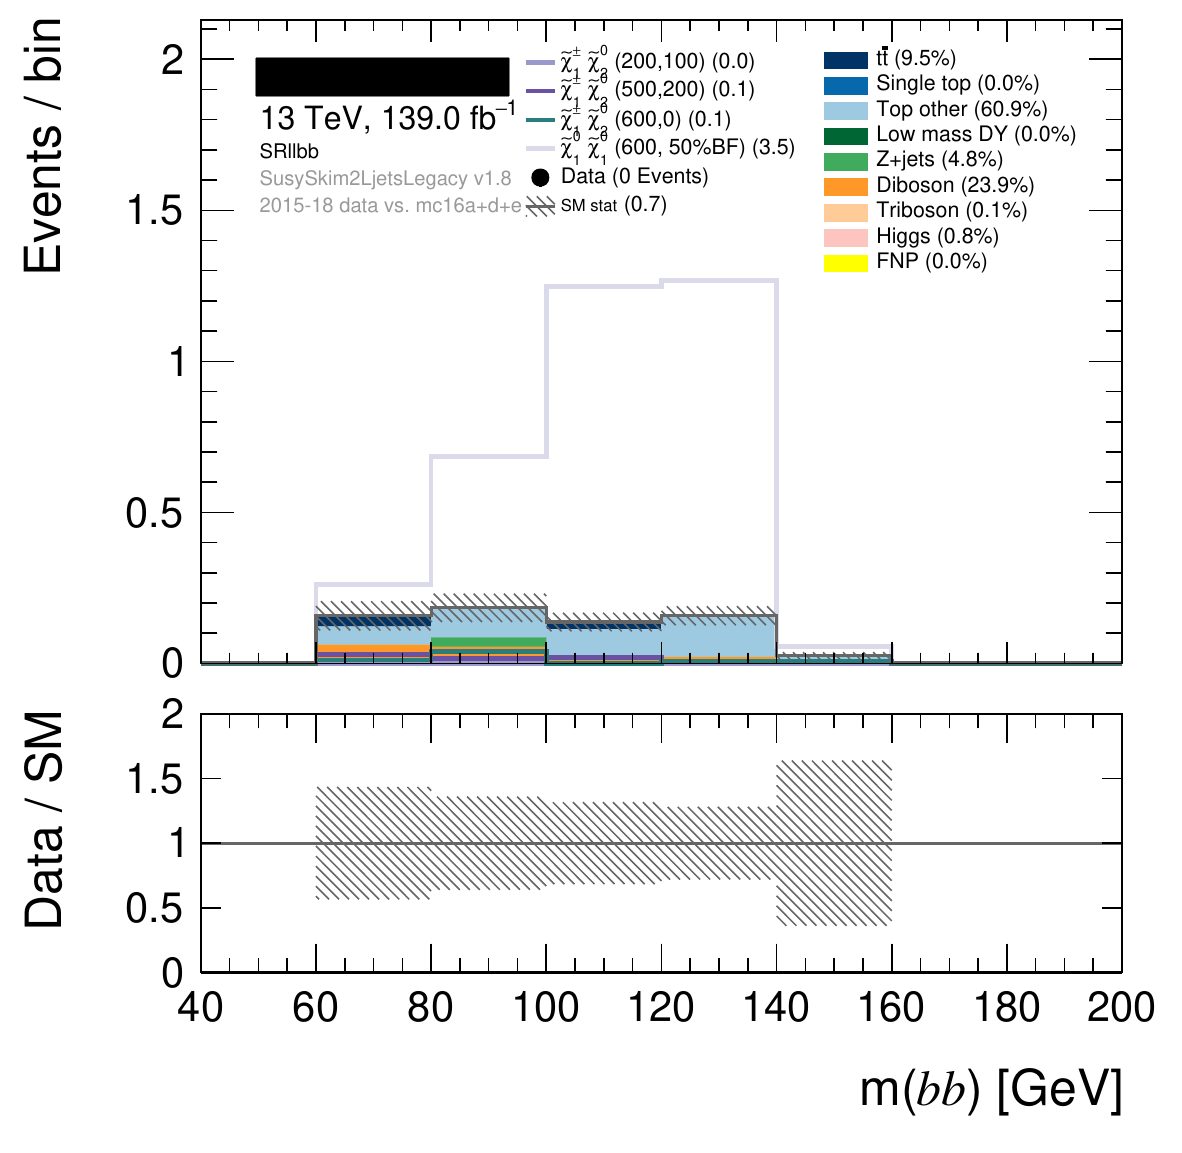
\includegraphics[width=\textwidth]{figures/2ljets_def_mbb_SRllbb.png}
\caption{\srllbb, $\mbb$}
\end{subfigure}
\\[0.4em]
\begin{subfigure}{0.495\textwidth}
\centering
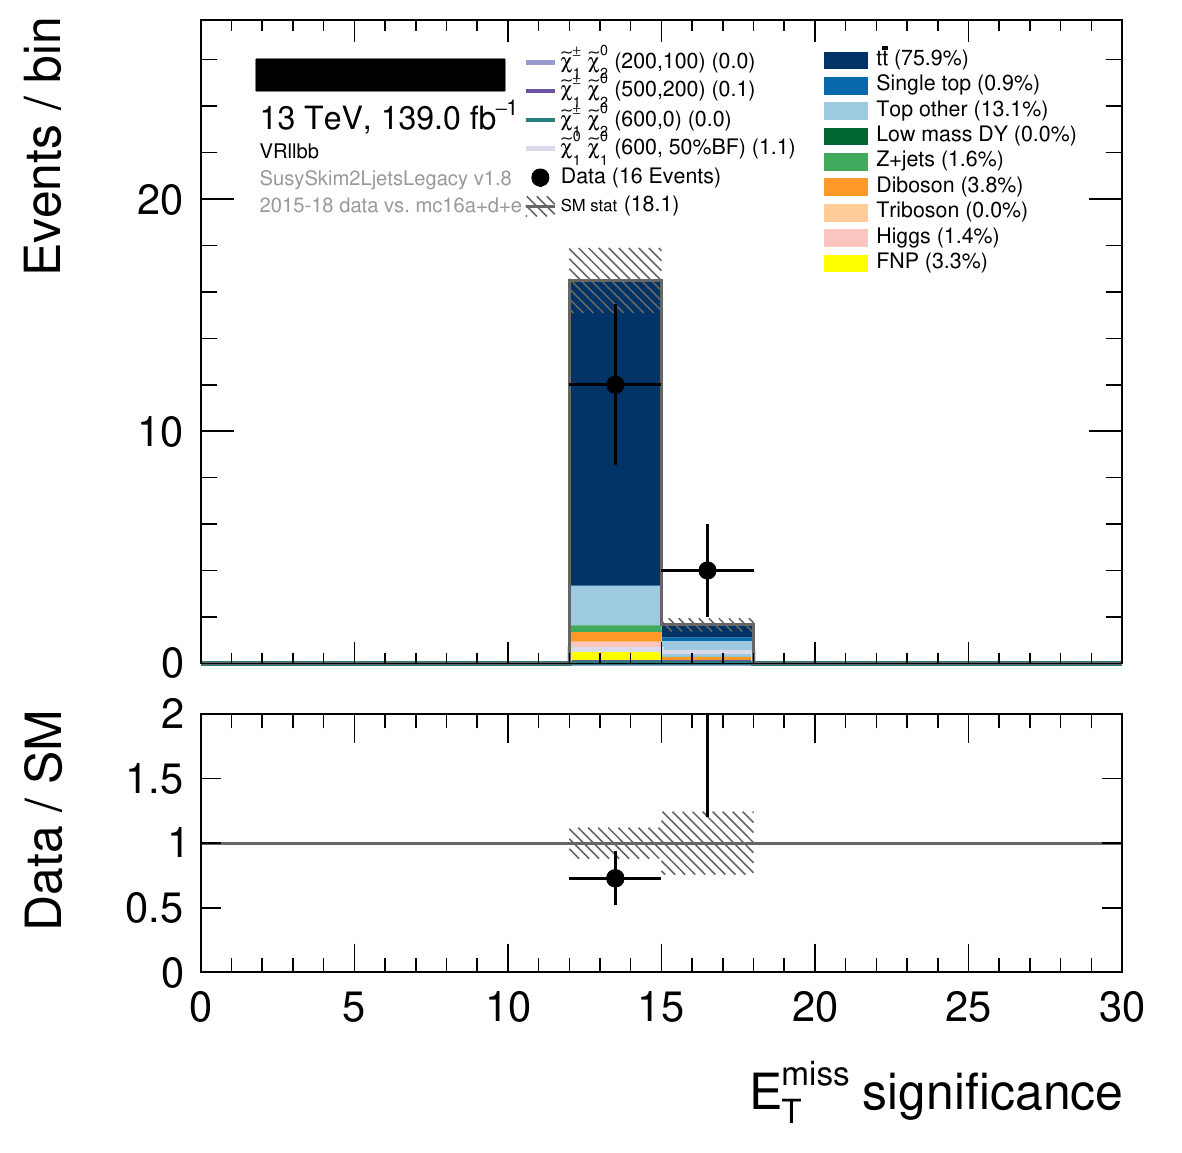
\includegraphics[width=\textwidth]{figures/2ljets_def_met_Sign_VRllbb.png}
\caption{VR-$\llbb$, $\metsig$}
\end{subfigure}
\hfill
\begin{subfigure}{0.495\textwidth}
\centering
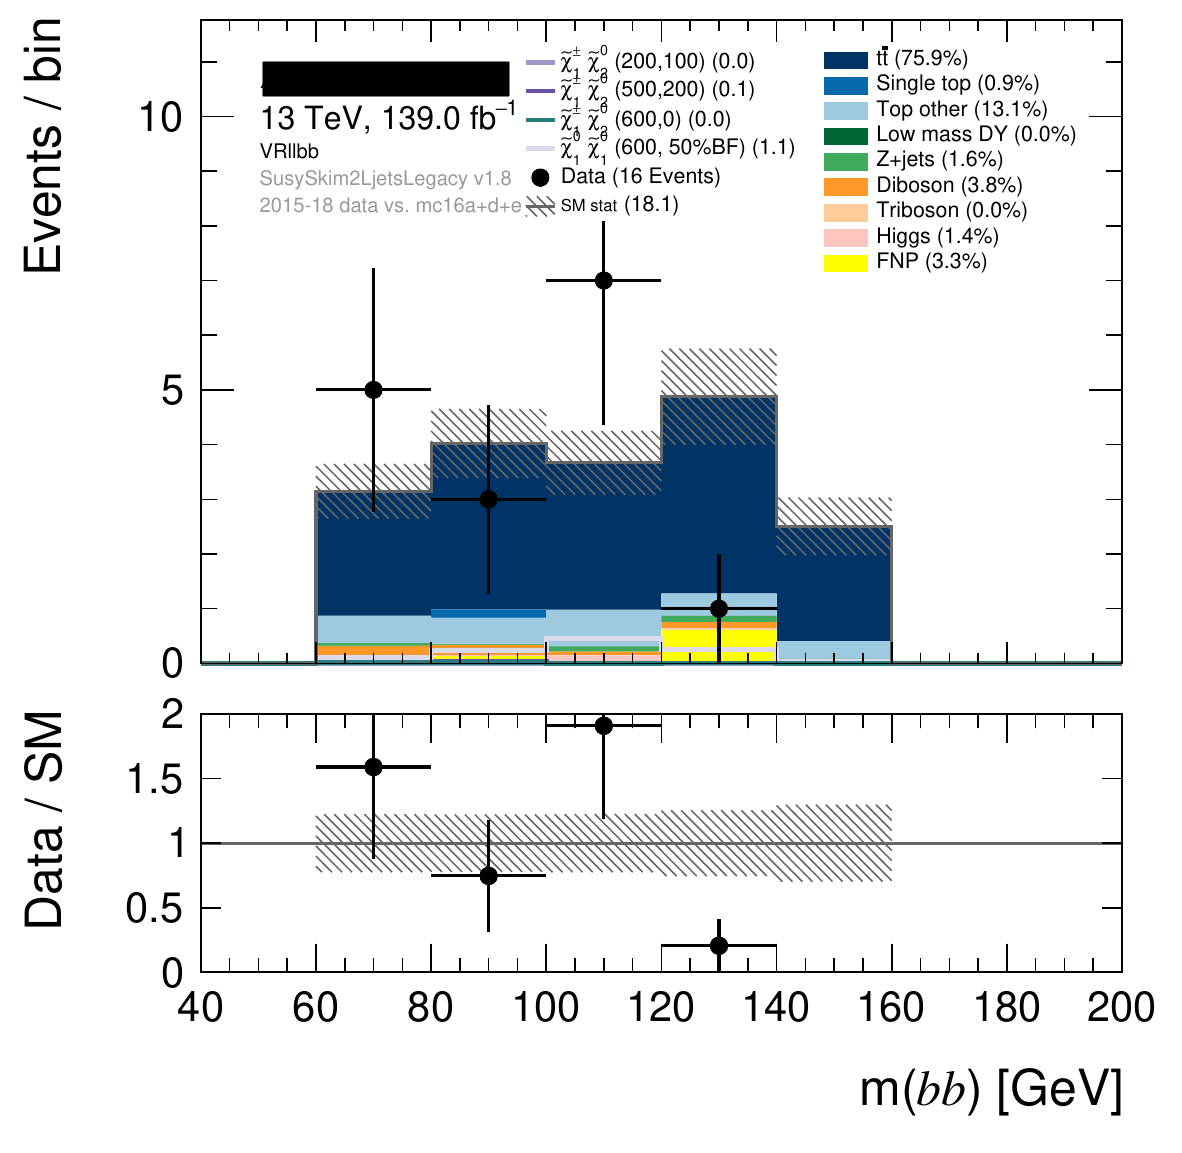
\includegraphics[width=\textwidth]{figures/2ljets_def_mbb_VRllbb.png}
\caption{VR-$\llbb$, $\mbb$}
\end{subfigure}
\caption[
Pre-fit distributions in $\llbb$ signal and validation regions
]{%
Pre-fit distributions in $\llbb$ signal and validation regions.
Signal regions are unblinded.
Errors are statistical.
}
\label{fig:2ljets_high_llbb_region}
\end{figure}

Validation regions, as always, are defined near to each signal region, under
the constraint of being somehow `nearby' and having enough data to test
background predictions.
For SR-High, inverting the selections on $\mjj$ or $\rjj$ satisfies
these criteria, so one validation region is designed on each.
An apparent excess appears at small $\mjj$ in VR-High, which is shown in
Figure~\ref{fig:2ljets_high_mjj_vrhigh}.
Various validation studies explored similar selections and different
simulated samples, and found no clear explanation for this effect.
The resulting doubt in our modelling of light jet pairs also therefore motivates
the second validation region VR-High-R, and the inclusion of a lower bound of
$\mjj > 20\,\eV[G]$ in all regions.
As seen in Figures~\ref{fig:2ljets_high_region}
and~\ref{fig:2ljets_high_mjj_vrhigh}, VR-High and VR-High-R otherwise show
acceptable pre-fit modelling even without the inclusion of systematic
uncertainties in their error bars.

\begin{figure}[tp]
\centering
\begin{subfigure}{0.495\textwidth}
\centering
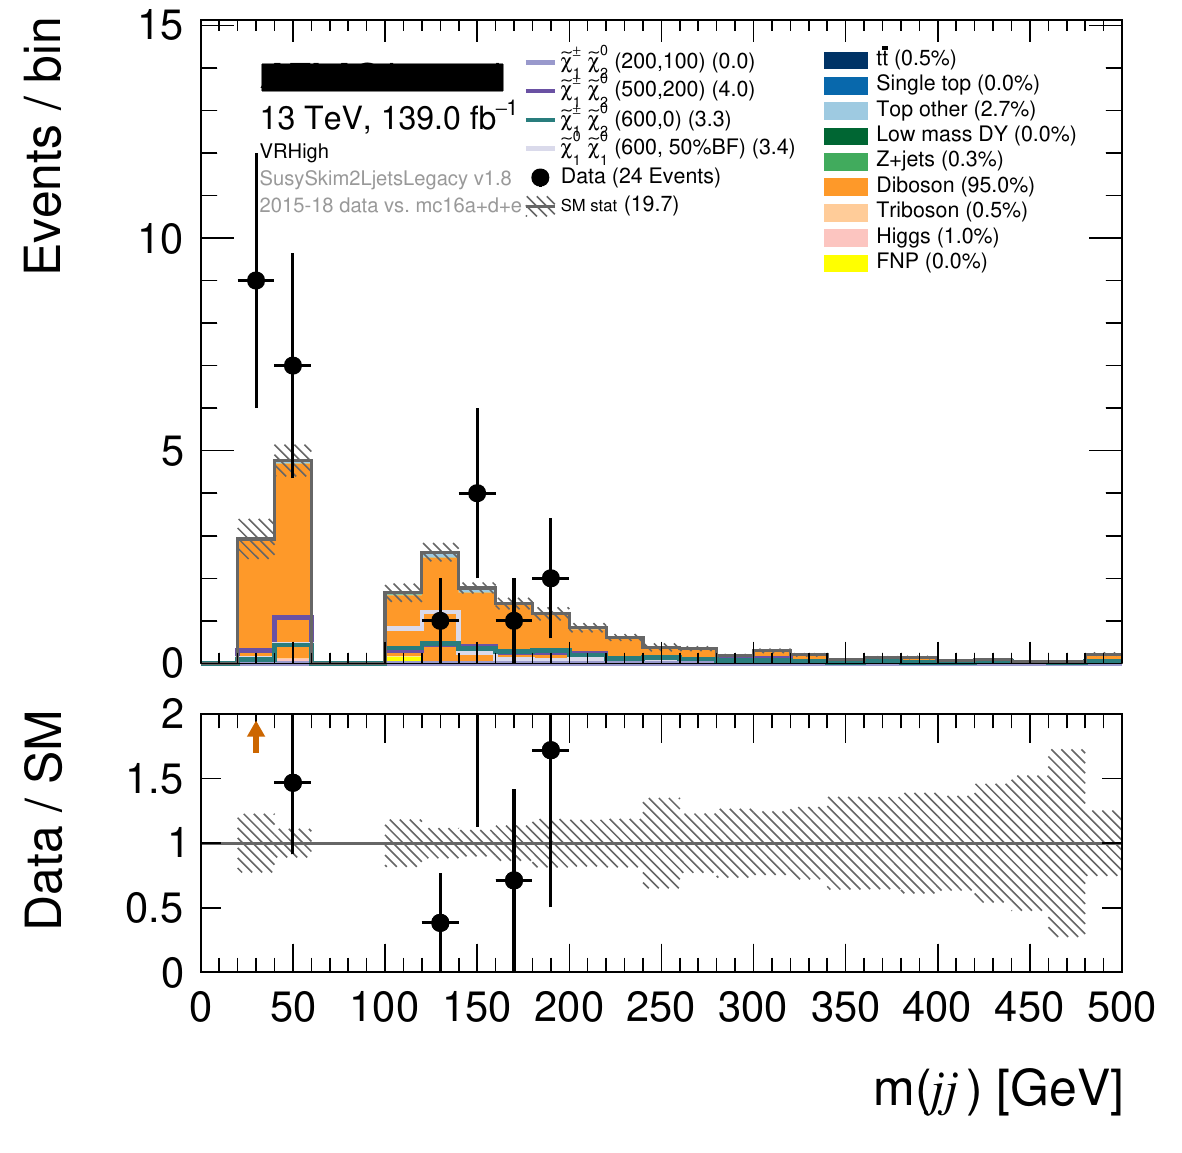
\includegraphics[width=\textwidth]{figures/2ljets_def_mjj_VRHigh.png}
\caption{VR-High, $\mjj$}
\end{subfigure}
\hfill
\begin{subfigure}{0.495\textwidth}
\centering
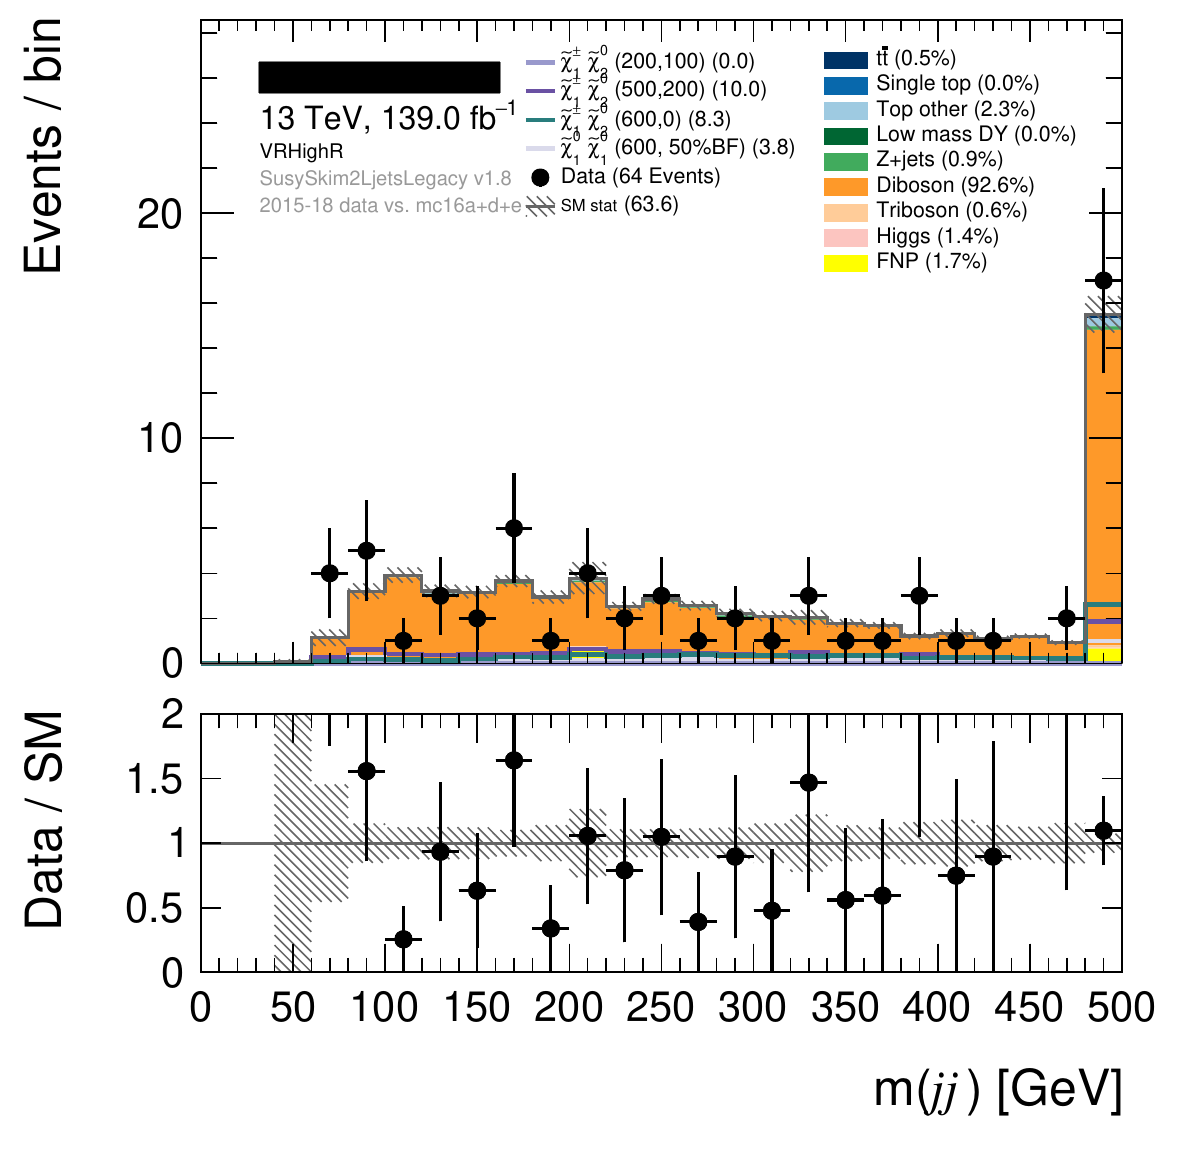
\includegraphics[width=\textwidth]{figures/2ljets_def_mjj_VRHighR.png}
\caption{VR-High-R, $\mjj$}
\end{subfigure}
\caption[
Pre-fit $\mjj$ distributions in validation regions VR-High and VR-High-R
]{%
Pre-fit $\mjj$ distributions in validation regions VR-High and VR-High-R.
Signal regions are unblinded.
Errors are statistical.
The apparent excess at low $\mjj$ in VR-High is not well understood.
}
\label{fig:2ljets_high_mjj_vrhigh}
\end{figure}

The distribution of mono-jet masses ($\mjetone$) is sharply peaked towards zero,
so cutting this out while inverting the $\mjetone$ selection of SR-High-1J
more clearly inspects the modelling of massive jets, which appears to be good.
Note that the region $\mjetone > 110$ is also checked in this validation region
and seen to contain no data --- a good sign for the Standard Model.
Since background estimates are near zero up there, non-zero data would have
ruled out our modelling in favour of any plausible model that made small
positive predictions.

The small yields beside \srllbb\ in other event variables left $\metsig$ as
the only appropriate candidate to change for VR-$\llbb$.
Unfortunately, this region mostly checks $\ttbar$ backgrounds, and not the
rare $\ttbar Z$ backgrounds which we would most like to validate.
Early work observed good $\ttbar Z$ modelling in three- and four- lepton
selections, but these were excluded from the $\twoljets$ analysis for
orthogonality from other \atlas\ searches with which our results are to be
combined in future.

Overall, the total background yield predict the data well in VR-$\llbb$.
What was not appreciated soon enough, however, was an excess in the $\metsig$
tail of this region, which is shown in the $\twoljets$ paper and reproduced
Figure~\ref{fig:2ljets_high_metsig_vrllbb_paper}.
The highest bins have small background predictions and positive data.
Had this been noticed before unblinding, more validation studies or altered
modelling might have been necessary.
``In the end'', commented one \atlas\ author~\cite{comment2022vrllbb},
``it seems fine since there's not events in the SR!''

\begin{figure}[tp]
\centering
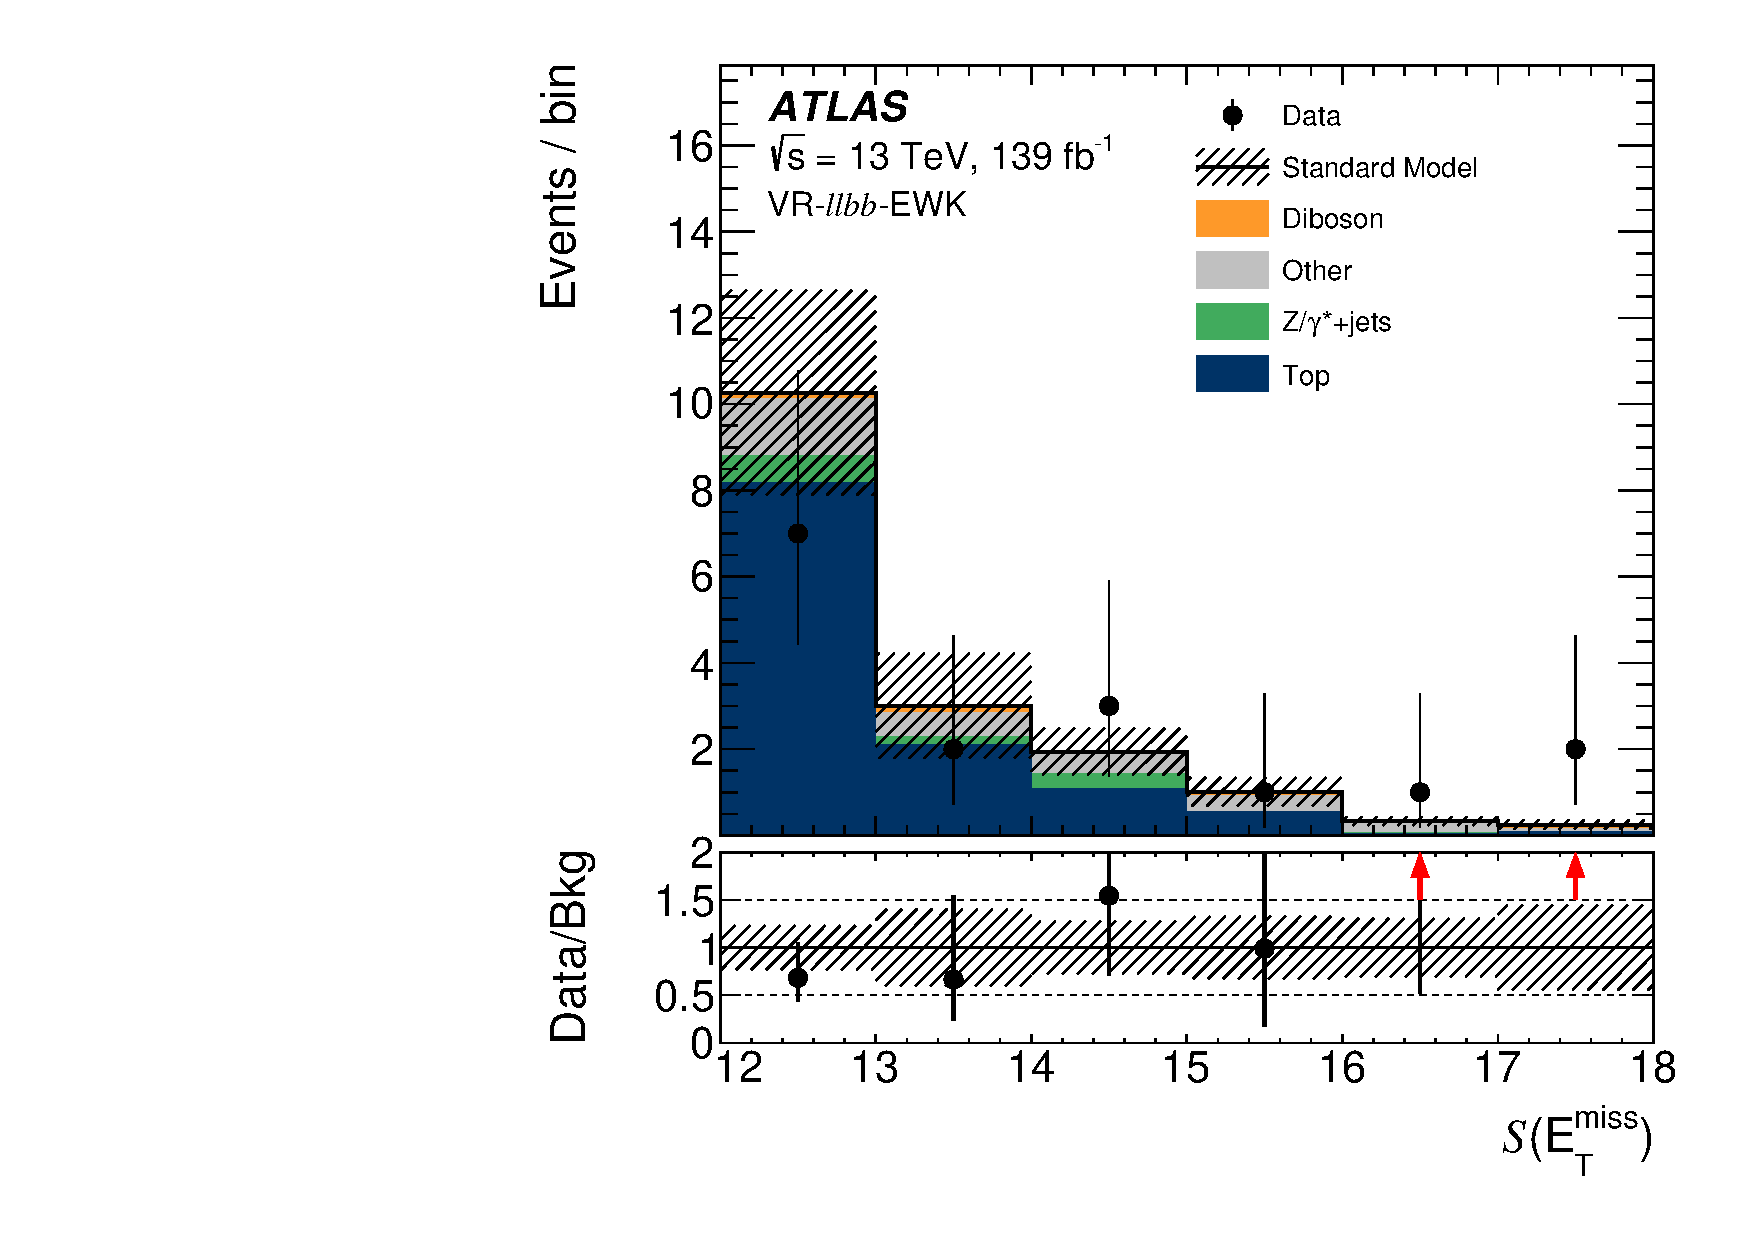
\includegraphics[width=0.62\textwidth]{figures/2ljets_vr_llbb_met_sig.pdf}
\caption[
Post-fit $\metsig$ distribution in VR-$\llbb$
]{%
Post-fit $\metsig$ distribution in VR-$\llbb$ with all statistical and
systematic uncertainties~\cite{atlas2022searches}.
Backgrounds are fitted to control and signal regions.
This region is also displayed pre-fit with coarser bins in
Figure~\ref{fig:2ljets_high_llbb_region}.
}
\label{fig:2ljets_high_metsig_vrllbb_paper}
\end{figure}


\subsection{Intermediate}
\label{sec:2ljets_int}
Our Intermediate signal regions sit in the $\metsig$ range of
$12$ to $18$.
As seen from Figure~\ref{fig:2ljets_presel_met}, this space suffers from
$\ttbar$ background contributions, but it also receives substantial signal
yields from some lighter signal models.
The larger rates of background processes in this space also make it ripe for
control regions.

Intermediate signal regions are defined in Table~\ref{tab:2ljets_int},
along with their associated validation regions and the control regions in this
space.
To suppress the increased backgrounds, the intermediate $\mll$ window is
tightened to reduce non-$Z$ backgrounds, including $\ttbar$ and \diboson\
processes.
Requiring zero $b$-tags further reduces $\ttbar$ backgrounds here.

\begin{table}[tp]
\centering
\begin{tabular}{lccccc}
& $\njet$
& $\nbtag$
& $\metsig$
& $\mjj$
& $\ptjone$
\\[1em]
SR-Int
& $\geq 2$
& $\hphantom{\geq}~0$
& $12\textrm{--}15\textrm{--}18$
& $60\textrm{--}110$
& $> 60$
\\[0.4em]
\: VR-Int
& $\geq 2$
& $\hphantom{\geq}~0$
& $12\textrm{--}18$
& $60\textrm{--}110$
& $\uwave{< 60}$
\\[1em]
\crvz
& $\geq 2$
& $\hphantom{\geq}~0$
& $12\textrm{--}18$
& $\uwave{20\textrm{--}60 \mid 110\textrm{--}\infty}$
& $\uwave{\hphantom{< 60}}$
\\[0.4em]
\crtt
& $\geq 2$
& $\uwave{\geq 1}$
& $\uwave{9\textrm{--}12}$
& $\uwave{20}$
& $> 60$
\end{tabular}
\\[1em]
Common: Pre-selection,
$\njet \geq 2$,
$\mll \in 81\textrm{--}101$, and
$\mttwoll > 80$.
\caption[
Intermediate region definitions in the $\twoljets$-electroweak analysis
]{%
Intermediate region definitions in the $\twoljets$-electroweak analysis.
En-dashes `$a\textrm{--}b$' indicate open intervals $(a, b)$.
Concatenated intervals `$a\textrm{--}b\textrm{--}c$' indicate binning
with boundaries at $a$, $b$, and $c$.
The mid-bar `$\mid$' indicates logical `or'.
Differences between regions are \uwave{underlined}.
}
\label{tab:2ljets_int}
\end{table}

The less extreme signal models targeted here have less boosted
$W\to jj$ distributions, but a $\ptjone$ selection is found to be
effective as an additional discriminator of signals from backgrounds to make
up for this loss;
a $\ptjone > 60\,\eV[G]$ requirement splits SR-Int from its validation region
VR-Int, and is seen from Figure~\ref{fig:2ljets_int_region} to keep most
signal contributions in the signal region.
Following our standard pattern set with other signal regions, SR-Int is binned
in $\metsig$ in intervals of $3$ units to improve signal sensitivity.

\begin{figure}[tp]
\centering
\begin{subfigure}{0.495\textwidth}
\centering
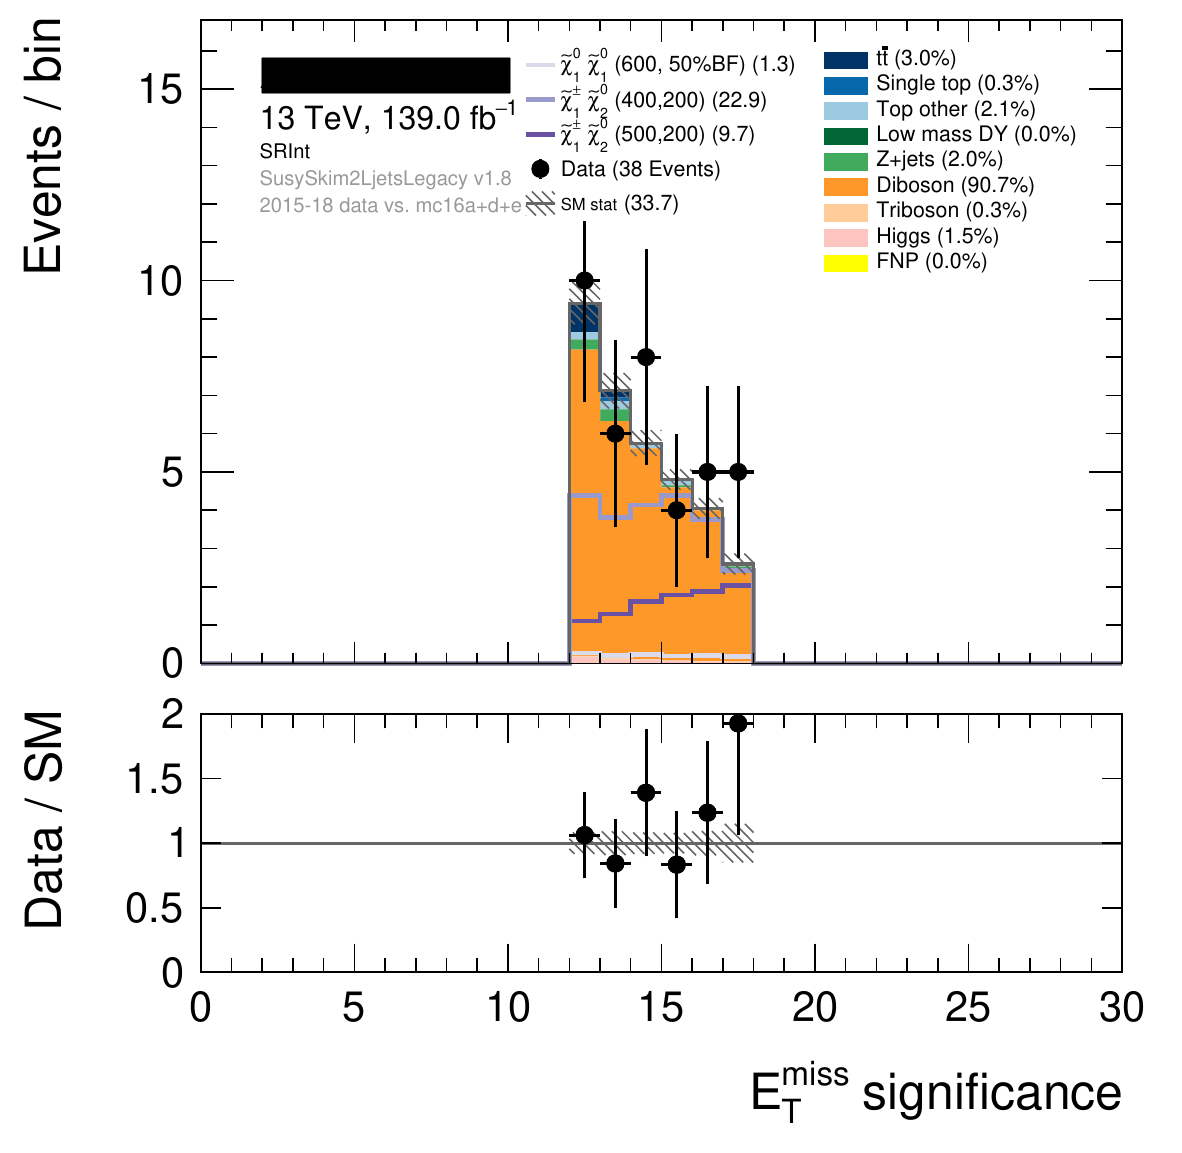
\includegraphics[width=\textwidth]{figures/2ljets_def_met_Sign_SRInt.png}
\caption{SR-Int, $\metsig$}
\end{subfigure}
\hfill
\begin{subfigure}{0.495\textwidth}
\centering
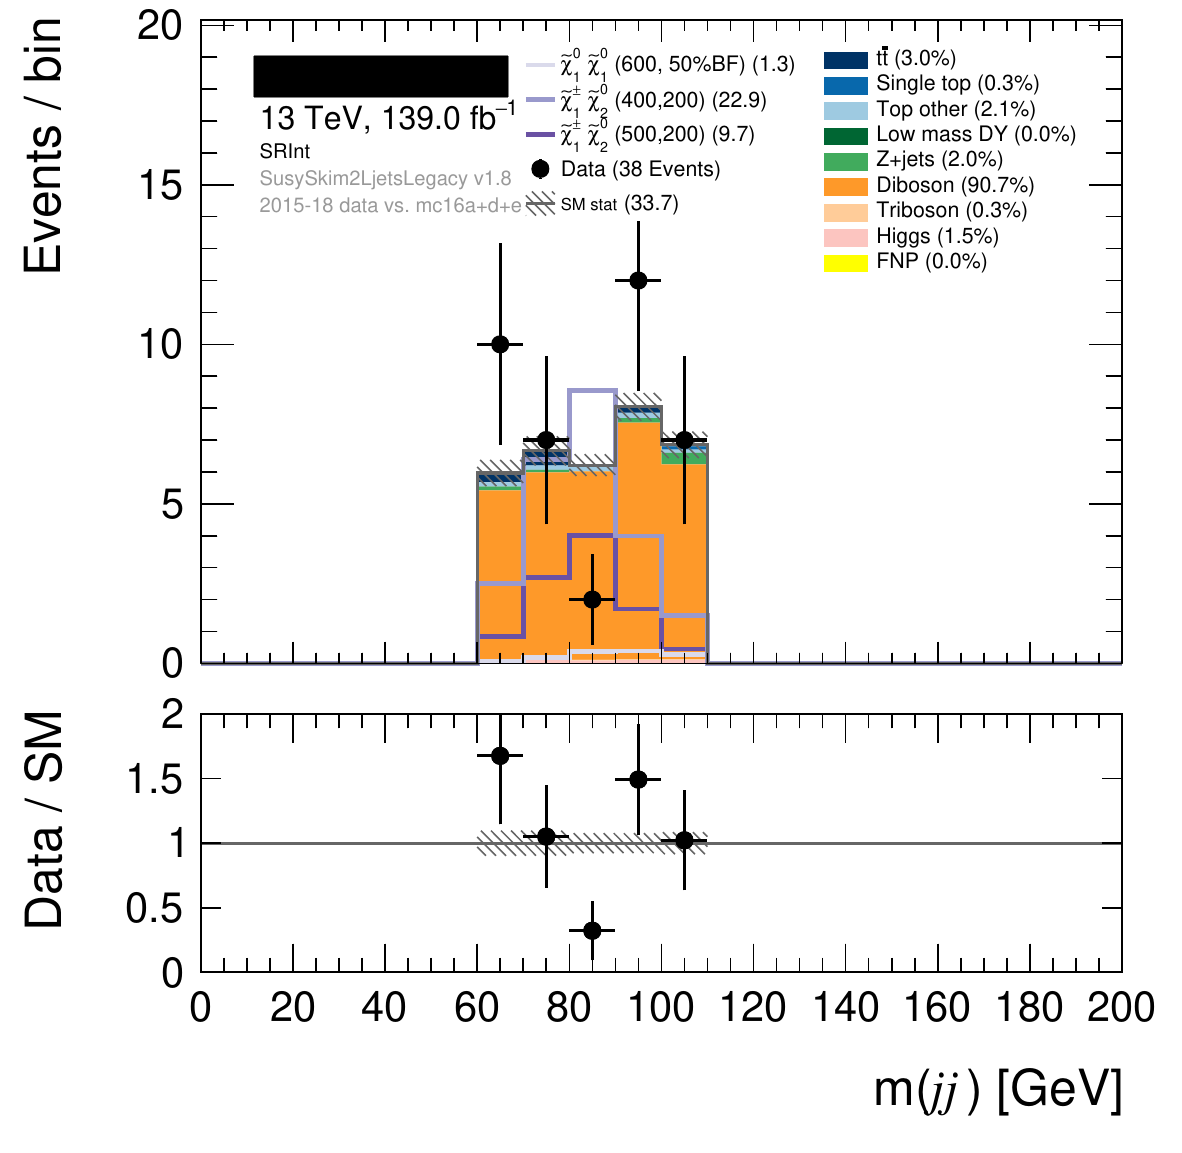
\includegraphics[width=\textwidth]{figures/2ljets_def_mjj_SRInt.png}
\caption{SR-Int, $\mjj$}
\end{subfigure}
\\[0.4em]
\begin{subfigure}{0.495\textwidth}
\centering
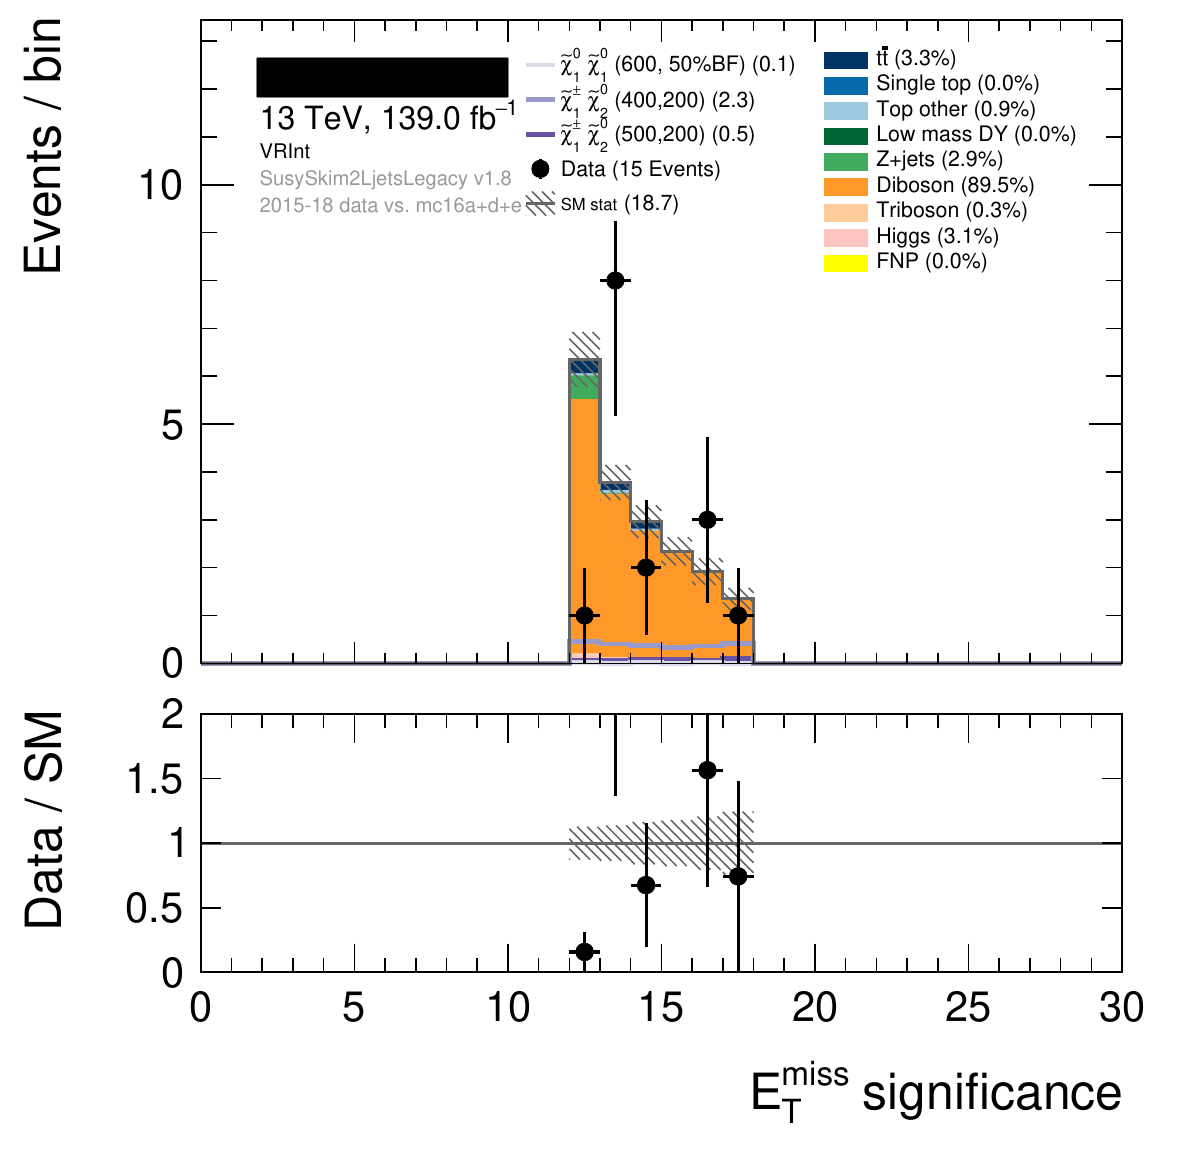
\includegraphics[width=\textwidth]{figures/2ljets_def_met_Sign_VRInt.png}
\caption{VR-Int, $\metsig$}
\end{subfigure}
\hfill
\begin{subfigure}{0.495\textwidth}
\centering
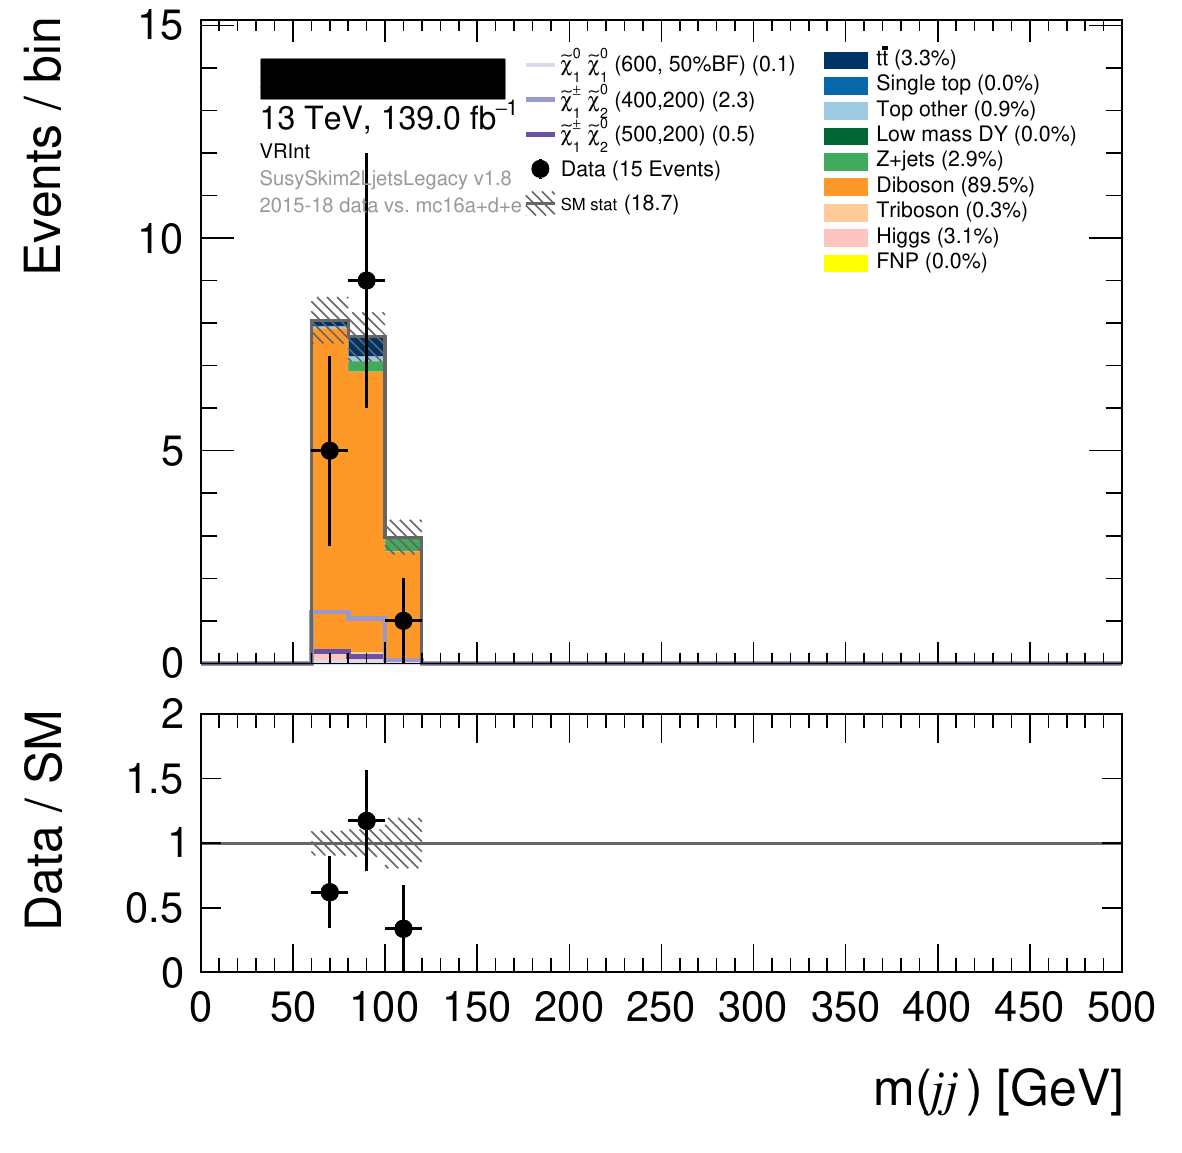
\includegraphics[width=\textwidth]{figures/2ljets_def_mjj_VRInt.png}
\caption{VR-Int, $\mjj$}
\end{subfigure}
\caption[
Pre-fit distributions in Intermediate signal and validation regions
]{%
Pre-fit distributions in Intermediate signal and validation regions.
Signal regions are unblinded.
Errors are statistical.
}
\label{fig:2ljets_int_region}
\end{figure}

The control region \crvz\ occupies the $\mjj$ sideband of SR-Int and VR-Int.
As seen from Figure~\ref{fig:2ljets_int_cr_region}, the selections in this
intermediate space give \crvz\ a very pure \diboson\ background, which is
valuable to constrain our modelling by extrapolation to High regions.
Also included in Table~\ref{tab:2ljets_int} and
Figure~\ref{fig:2ljets_int_cr_region} is \crtt, which uses various other
selections of $b$-tagged data to constrain $\ttbar$ backgrounds.
Both control regions show good agreement pre-fit and with statistical uncertainties
only.
\begin{figure}[tp]
\centering
\begin{subfigure}{0.495\textwidth}
\centering
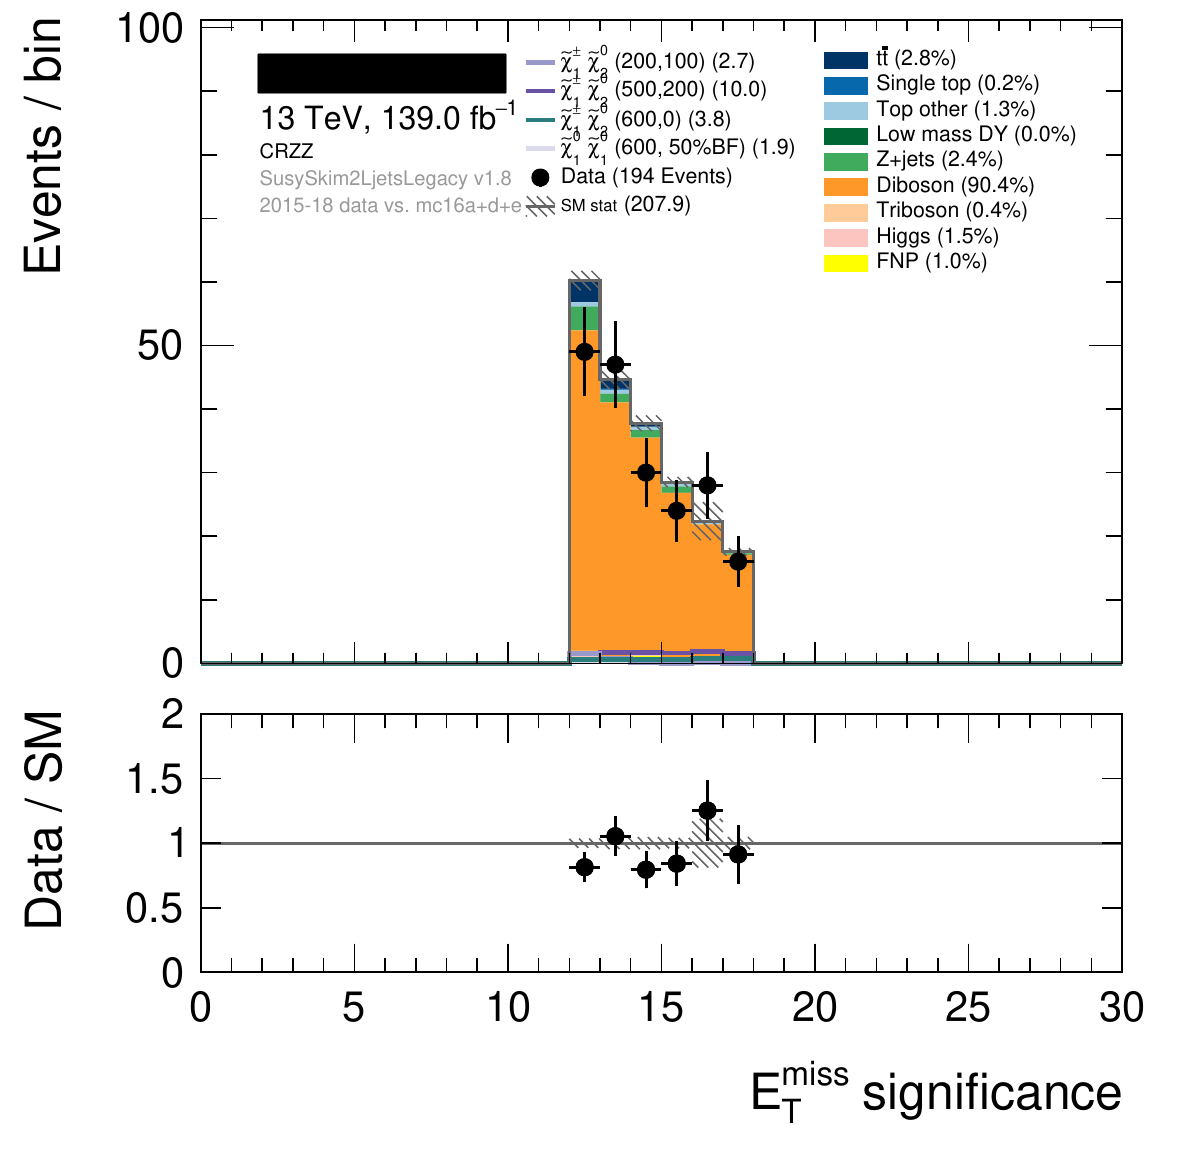
\includegraphics[width=\textwidth]{figures/2ljets_def_met_Sign_CRZZ.png}
\caption{\crvz, $\metsig$}
\end{subfigure}
\hfill
\begin{subfigure}{0.495\textwidth}
\centering
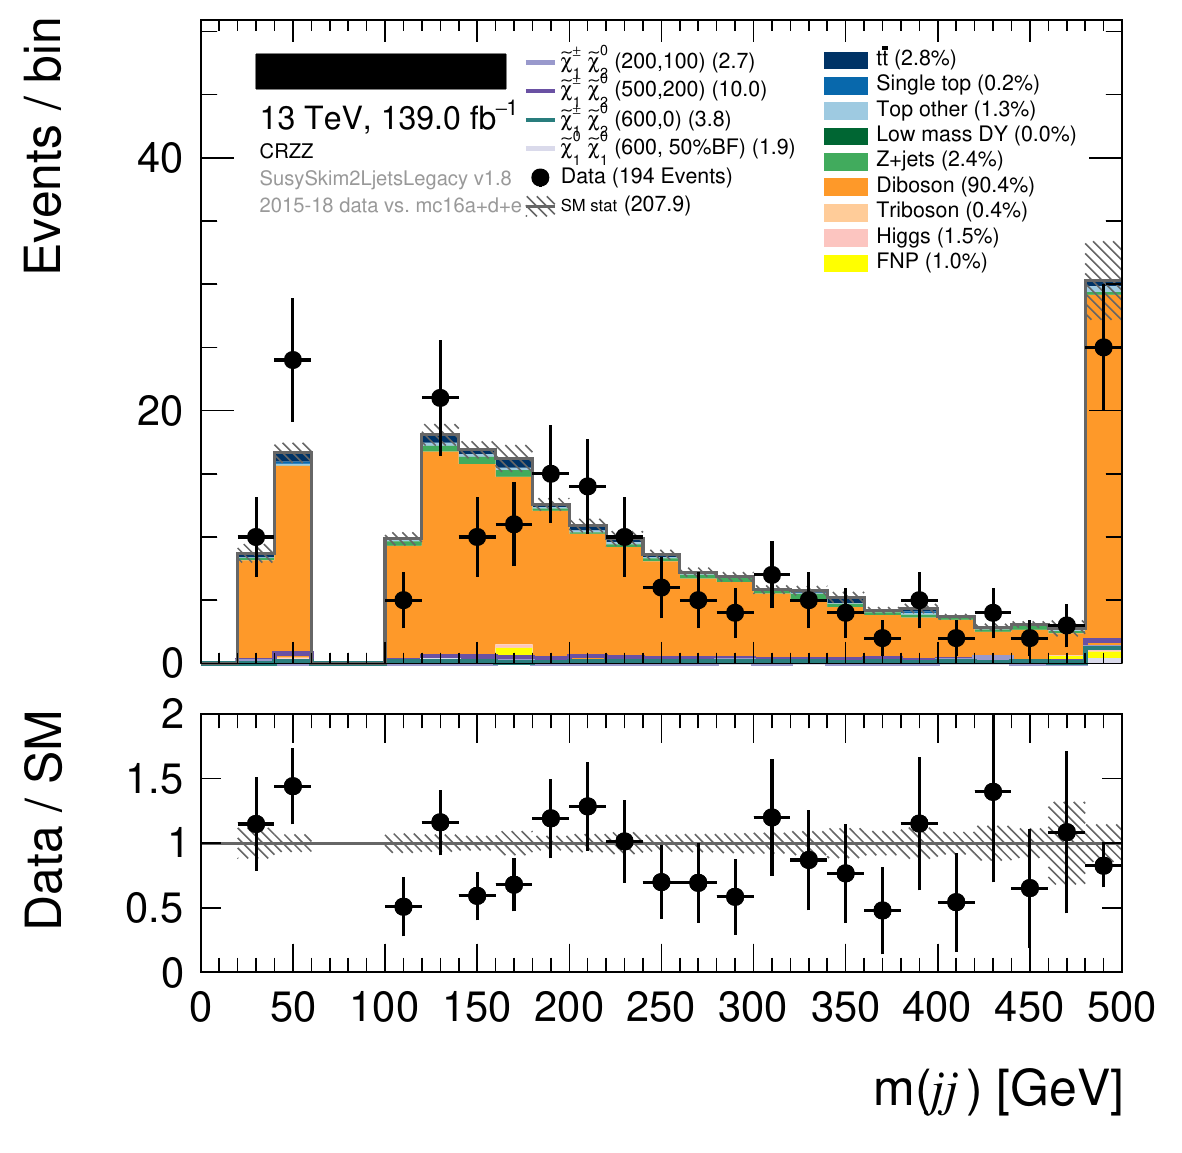
\includegraphics[width=\textwidth]{figures/2ljets_def_mjj_CRZZ.png}
\caption{\crvz, $\mjj$}
\end{subfigure}
\\[0.4em]
\begin{subfigure}{0.495\textwidth}
\centering
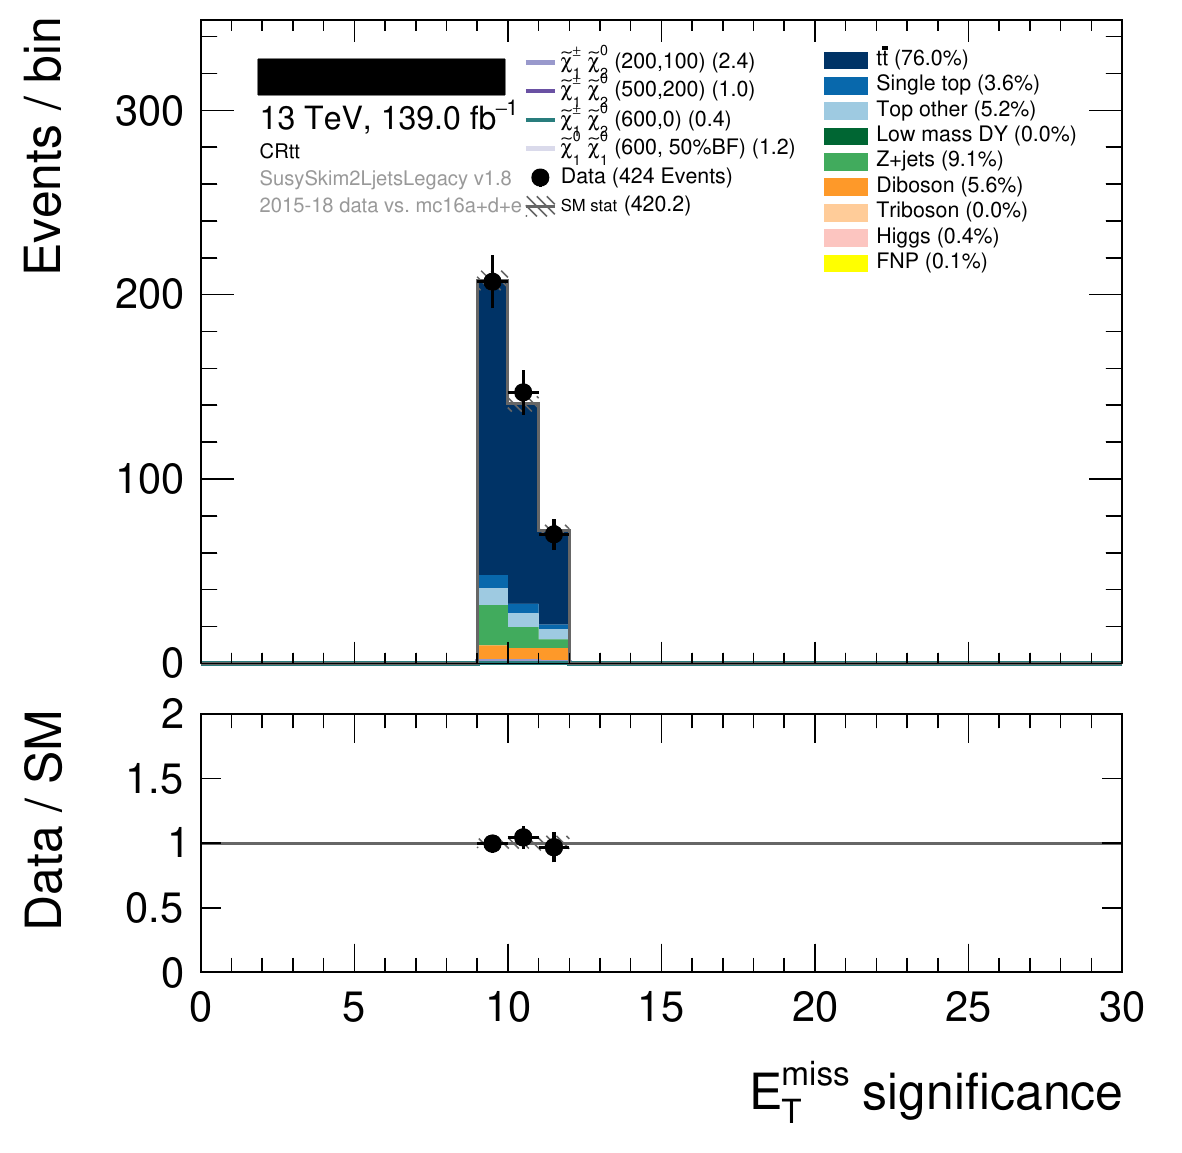
\includegraphics[width=\textwidth]{figures/2ljets_def_met_Sign_CRtt.png}
\caption{\crtt, $\metsig$}
\end{subfigure}
\hfill
\begin{subfigure}{0.495\textwidth}
\centering
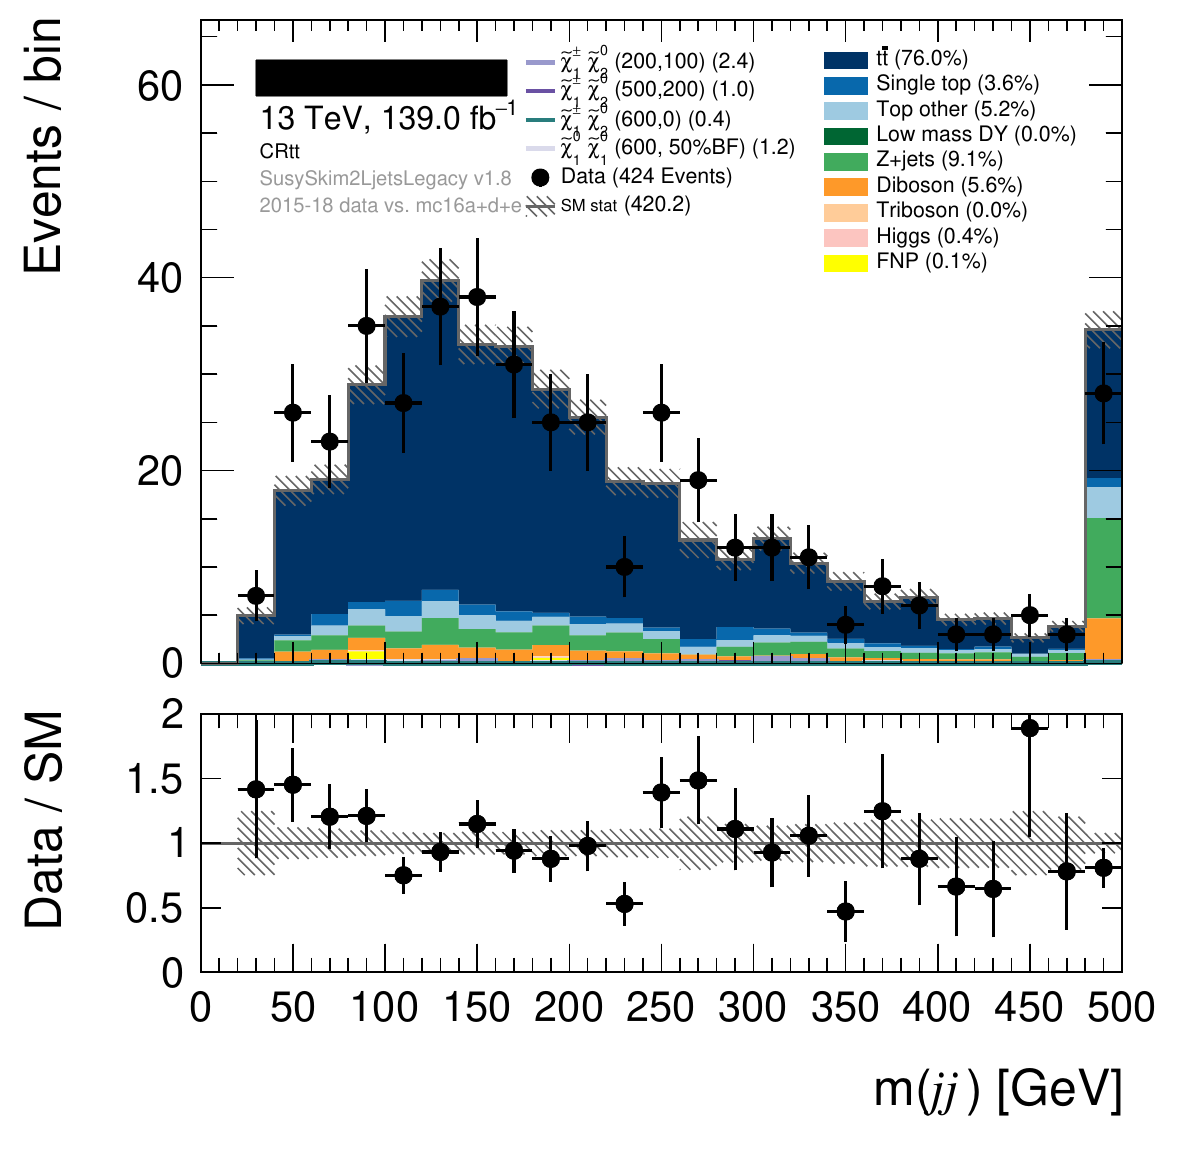
\includegraphics[width=\textwidth]{figures/2ljets_def_mjj_CRtt.png}
\caption{\crtt, $\mjj$}
\end{subfigure}
\caption[
Pre-fit distributions in the control regions CR-tt and CR-VZ
]{%
Pre-fit distributions in the control regions \crtt\ and \crvz.
Errors are statistical.
}
\label{fig:2ljets_int_cr_region}
\end{figure}

Some figures label \crvz\ as `\crz Z'; the region was renamed late in this
analysis project when it was shown to contain substantial fractions of
$W\kern-0.4exZ$ as well as $ZZ$, as illustrated in
Figure~\ref{fig:2ljets_splits} of
Section~\ref{sec:2ljets_validation}.


\subsection{Low}
\label{sec:2ljets_low}
In Low regions, which have $\metsig \in 6\textrm{--}12$, the $\zjets$
background becomes large since its fake $\met$, which arises from
mismeasurements or rare interactions, is no longer eliminated.
Backgrounds from $\ttbar$ similarly increase, and the selections inherited from
Intermediate regions are no longer sufficient.

These Low regions target signal models with small mass splittings of
$m(\chargino_1, \neutralino_2) - m(\neutralino_1)
\approx 100\textrm{--}150\,\eV[G]$ that still exceed the masses of
electroweak bosons.
In particular, we aim to test C1N2~($200$, $100$)
(meaning $m(\chargino_1, \neutralino_2) = 200\,\eV[G]$ and
$m(\neutralino_1) = 100\,\eV[G]$), which is a light on-shell benchmark that
has not previously been excluded in this channel~\cite{atlas_23l_SUSY_2016_24}.

Angular selections on lepton variables $\rll$ and $\dphillmet$ are powerful
in these Low regions, and characterize their definitions that
are given in Table~\ref{tab:2ljets_low}.
These angular variables usefully reject backgrounds including $\ttbar$, and
provide signal sensitivity to benchmark signal models, as illustrated in
Figure~\ref{fig:2ljets_low_minus}.

\begin{table}[tp]
\centering
\begin{tabular}{lcccccccc}
& $\metsig$
& $\mjj$
& $\mttwoll$
& $\rll$
& $\dphillmet$
\\[1em]
SR-Low
& $6\textrm{--}9\textrm{--}12$
& $60\textrm{--}110$
& $> 80$
& $< 1$
&
\\[0.4em]
\: VR-Low
& $6\textrm{--}12$
& $60\textrm{--}110$
& $>80$
& $\uwave{1\textrm{--}1.4}$
&
\\[1em]
SR-Low-2
& $6\textrm{--}9$
& $60\textrm{--}110$
& $< 80$
& $< 1.6$
& $< 0.6$
\\[0.4em]
\: VR-Low-2
& $6\textrm{--}9$
& $\uwave{20\textrm{--}60 \mid 110\textrm{--}\infty}$
& $< 80$
& $< 1.6$
& $< 0.6$
\\[1em]
\crz
& $6\textrm{--}9$
& $\uwave{20\textrm{--}60 \mid 110\textrm{--}\infty}$
& $> 80$
& $\uwave{\hphantom{< 1.6}}$
& $\uwave{\hphantom{< 0.6}}$
\end{tabular}
\\[1em]
Common: Pre-selection,
$\njet = 2$,
$\nbtag = 0$, and
$\mll \in 81\textrm{--}101$.
\caption[
Low region definitions in the $\twoljets$-electroweak analysis
]{%
Low region definitions in the $\twoljets$-electroweak analysis.
En-dashes `$a\textrm{--}b$' indicate open intervals $(a, b)$.
Concatenated intervals `$a\textrm{--}b\textrm{--}c$' indicate binning
with boundaries at $a$, $b$, and $c$.
The mid-bar `$\mid$' indicates logical `or'.
Differences between regions are \uwave{underlined}.
}
\label{tab:2ljets_low}
\end{table}

Boosted $Z\to \ell\ell$ decays will tend to have small $\rll$.
Similarly to $\rjj$ in the High regions, this can usefully select signals,
but here also works to reject other $\ell\ell$ production mechanisms that
produce leptons in less correlated directions, particularly dileptonic
$\ttbar$.
As elsewhere, sensitivity is increased by binning SR-Low
to form SR-Low-a with $\metsig \in 6\textrm{--}9$ and
SR-Low-b $\metsig \in 9\textrm{--}12$.

To remove some observed mis-modelling of backgrounds, Low regions require
exactly two jets.
Abandoned region designs, which used more jets, are discussed below in
Section~\ref{sec:2ljets_low_isr}.

Unblinded, pre-fit histograms of SR-Low are shown in
Figure~\ref{fig:2ljets_low_region}.
Note that these plots do not include systematic uncertainties, so the meaning
of the observed data deficits cannot yet be fully interpreted.
This figure also includes VR-Low, which observes the high $\rll$ edge and
predicts the data well.

\begin{figure}[tp]
\centering
\begin{subfigure}{0.495\textwidth}
\centering
\includegraphics[width=\textwidth]{figures/2ljets_low_Rll_SRLow_noRll.pdf}
\caption{SR-Low$/\{\rll\}$}
\end{subfigure}
\hfill
\begin{subfigure}{0.495\textwidth}
\centering
\includegraphics[width=\textwidth]{figures/2ljets_low_mt2leplsp_0_SRLow_noRll_nomt2.pdf}
\caption{SR-Low$/\{\rll,\mttwoll\}$}
\label{fig:2ljets_low_minus_norll_nomt2_mt2}
\end{subfigure}
\\[0.4em]
\begin{subfigure}{0.495\textwidth}
\centering
\includegraphics[width=\textwidth]{figures/2ljets_low_absdPhiPllMet_SRLow2_noDphi.pdf}
\caption{SR-Low-2$/\{\dphillmet\}$}
\label{fig:2ljets_low_minus_dphi}
\end{subfigure}
\hfill
\begin{subfigure}{0.495\textwidth}
\centering
\includegraphics[width=\textwidth]{figures/2ljets_low_absdPhiPllMet_SRLow2_noDphi_mg5.pdf}
\caption{SR-Low-2$/\{\dphillmet\}$ (alt)}
\label{fig:2ljets_low_minus_dphi_alt}
\end{subfigure}
\caption[
Relaxed versions of SR-Low and SR-Low-2 to motivate their angular selections
]{%
Relaxed versions of SR-Low and SR-Low-2 to motivate their angular selections.
Each removes requirements listed in Table~\ref{tab:2ljets_low}:
(a) SR-Low removes $\rll$,
(b) SR-Low removes $\rll$ and $\mttwoll$,
and
(c, d) SR-Low-2 removes $\dphillmet$.
\\[0.4em]
Signals trend towards small $\rll$, plausibly due to their more boosted
$Z\to \ell\ell$ decays; small $\rll$ also suppresses $\ttbar$.
The mass of signals seen at small $\mttwoll$ in (b) motivates the design of
SR-Low-2.
Signals in SR-Low-2 spike at small $\dphillmet$ in (c); better statistical
precision is provided by an alternative $\zjets$ sample in (d).
}
\label{fig:2ljets_low_minus}
\end{figure}

\begin{figure}[tp]
\centering
\begin{subfigure}{0.495\textwidth}
\centering
\includegraphics[width=\textwidth]{figures/2ljets_def_met_Sign_SRLow.png}
\caption{SR-Low, $\metsig$}
\end{subfigure}
\hfill
\begin{subfigure}{0.495\textwidth}
\centering
\includegraphics[width=\textwidth]{figures/2ljets_def_mjj_SRLow.png}
\caption{SR-Low, $\mjj$}
\end{subfigure}
\\[0.4em]
\begin{subfigure}{0.495\textwidth}
\centering
\includegraphics[width=\textwidth]{figures/2ljets_def_met_Sign_VRLow.png}
\caption{VR-Low, $\metsig$}
\end{subfigure}
\hfill
\begin{subfigure}{0.495\textwidth}
\centering
\includegraphics[width=\textwidth]{figures/2ljets_def_mjj_VRLow.png}
\caption{VR-Low, $\mjj$}
\end{subfigure}
\caption[
Pre-fit distributions in Low signal and validation regions
]{%
Pre-fit distributions in Low signal and validation regions.
Signal regions are unblinded.
Errors are statistical.
}
\label{fig:2ljets_low_region}
\end{figure}

Uniquely to Low regions and signal models with small mass-splitting, it is
found, and shown in Figure~\ref{fig:2ljets_low_minus_norll_nomt2_mt2}, that
substantial signal yields exist above backgrounds at small $\mttwoll$.
To capture these signals, SR-Low-2 is defined as the only
$\twoljets$-electroweak region with $\mttwoll < 80\,\eV[G]$.
That precise threshold of $80\,\eV[G]$ is not very important, and used only to make it
a simple inversion of the usual $\mttwoll > 80\,\eV[G]$ requirement.
After the other selections for SR-Low-2, almost all signal and background
samples are in the spike near zero;
a lower requirement would make little difference and work just as well,

As shown in Figure~\ref{fig:2ljets_low_minus_dphi}, signal models peak at small
$\dphillmet$, and backgrounds do not; this motivates the $\dphillmet < 0.6$
requirement, and can be plausibly understood from scenarios where a boosted
supersymmetric resonance decays to $Z+\mathrm{invisible}$ and sends both
the $Z\to \ell\ell$ and invisible particle, which becomes
$\ptmiss$, in the same direction.

The distribution $\zjets$ here may be surprising, since its $\ptmiss$ is
expected to usually align with a mismeasured jet.
This is explained by the context of the $\mttwoll < 80\,\eV[G]$
requirement:
if $\ptmiss$ is facing away from both leptons, then they have large transverse
masses.
Following its definition as a $\min-\max$ of transverse masses from
Section~\ref{sec:2ljets_mt2},
the $\mttwoll$ requirement therefore rejects those events, leaving only the
rarer cases of $\zjets$ with small $\dphillmet$.

Excluding $\metsig \in 9\textrm{--}12$ in SR-Low-2 is also not crucial.
This space contains about $2.3$ background expectation (mostly \diboson) and
around $1$ expected event from some benchmark signals, so its inclusion as a
single combined bin might not have increased sensitivity.
Its inclusion as an orthogonal bin with small yields would also have added
unnecessary complication with little benefit.

Histograms of SR-Low-2 are shown in Figure~\ref{fig:2ljets_low2_region}.
To get sufficiently large backgrounds, the validation region VR-Low-2 uses
the $\mjj$ sideband, and sees good agreement.

\begin{figure}[tp]
\centering
\begin{subfigure}{0.495\textwidth}
\centering
\includegraphics[width=\textwidth]{figures/2ljets_def_met_Sign_SRLow2.png}
\caption{SR-Low-2, $\metsig$}
\end{subfigure}
\hfill
\begin{subfigure}{0.495\textwidth}
\centering
\includegraphics[width=\textwidth]{figures/2ljets_def_mjj_SRLow2.png}
\caption{SR-Low-2, $\mjj$}
\end{subfigure}
\\[0.4em]
\begin{subfigure}{0.495\textwidth}
\centering
\includegraphics[width=\textwidth]{figures/2ljets_def_met_Sign_VRLow2.png}
\caption{VR-Low-2, $\metsig$}
\end{subfigure}
\hfill
\begin{subfigure}{0.495\textwidth}
\centering
\includegraphics[width=\textwidth]{figures/2ljets_def_mjj_VRLow2.png}
\caption{VR-Low-2, $\mjj$}
\end{subfigure}
\caption[
Pre-fit distributions in Low-2 signal and validation regions
]{%
Pre-fit distributions in Low-2 signal and validation regions.
Signal regions are unblinded.
Errors are statistical.
}
\label{fig:2ljets_low2_region}
\end{figure}

Sadly, the $\zjets$ background in SR-Low-2 has terrible statistical precision
in the central simulated sample due to large weights.
This was not as bad when the region was first designed, but became exaggerated
after reprocessing with a new lepton definition and updated software.
The region is plotted with an alternative sample in
Figure~\ref{fig:2ljets_low_minus_dphi_alt}, which has better precision.

% CR
The $\zjets$ control region \crz\ is displayed in
Figure~\ref{fig:2ljets_low_cr_region}.
Pre-fit agreement with data is quite good, although the overflow bin has a
notable excess.
Standardizing selections to remove high-$\mjj$ tails (such as requiring
$\mjj < 500\,\eV[G]$) could have made control and validation regions like \crz\
kinematically closer to the signal regions they are supposed to target,
and such a selection may well have improved the analysis in this case.

\begin{figure}[tp]
\centering
\begin{subfigure}{0.62\textwidth}
\centering
\includegraphics[width=\textwidth]{figures/2ljets_def_met_Sign_CRZ.png}
\caption{\crz, $\metsig$}
\end{subfigure}
\\
\begin{subfigure}{0.62\textwidth}
\centering
\includegraphics[width=\textwidth]{figures/2ljets_def_mjj_CRZ.png}
\caption{\crz, $\mjj$}
\end{subfigure}
\caption[
Pre-fit distributions in the control region CR-Z
]{%
Pre-fit distributions in the control region \crz.
Errors are statistical.
}
\label{fig:2ljets_low_cr_region}
\end{figure}

The gap in \crz\ at $\mjj \in 60\textrm{--}110\,\eV[G]$ is exactly SR-Low;
their union therefore has a continuous $\mjj$ distribution that is displayed
in Figure~\ref{fig:2ljets_low_sr_or_cr_region}.
Looking at the signal region alone can give an impression that $\zjets$ is
overestimated.
This plot contradicts that: most of the $\zjets$ distribution is fine;
the strange data deficit is local to $\mjj \approx m(W)$, which is where the
\diboson\ sample contributes a majority of the simulated background.

\begin{figure}[tp]
\centering
\includegraphics[width=0.8\textwidth]{figures/2ljets_low_mjj_SRLow_or_CRZ.pdf}
\caption[
The union of CR-Z and SR-Low
]{%
The union of \crz\ and SR-Low, which exactly fills its gap at
$\mjj \in 60\textrm{--}110\,\eV[G]$.
Data have a substantial dip in exactly that mass window.
Errors are statistical.
}
\label{fig:2ljets_low_sr_or_cr_region}
\end{figure}


\subsubsection{Low-ISR}
\label{sec:2ljets_low_isr}
The Low regions presented in Section~\ref{sec:2ljets_low} resulted from a
hasty redesign shortly before unblinding.
Before that redesign, a multi-jet signal region SR-Low-ISR was included,
with associated validation and control regions
that required $\njet \geq 3$ and offered some meagre extra sensitivity.
Here, `ISR' stands for Initial-State Radiation, following the naming
of previous \atlas\ searches including the partial Run~2 $2\ell$/$3\ell$
search, which we are updating~\cite{atlas_23l_SUSY_2016_24} in the
$\twoljets$-electroweak search.
Although these Low-ISR regions were removed from the analysis and we never
inspected the data in SR-Low-ISR (never unblinded), I include them here because
they reveal some interesting context to the surviving analysis design.
Specifically, prototype validation regions for Low-ISR designs revealed some
bad modelling by our Standard Model background samples in phase space that is
close to SR-Low, which is a region where we observe significant data deficits.
Secondly, these regions were an impactful part of the analysis design process
and led to the final design of SR-Low;
describing my experiences with them therefore reveals more about the true
design process.

Although initial-state radiation often refers to soft emissions in
parton showers~\cite{corcella2000initial, bewick2022initial},
our ISR explicitly includes hard emissions from the perturbative matrix element
simulation.
Our ISR is selected to give a hard transverse boost to the supersymmetric
particles, making their resulting $\met$ more distinctive.

To select ISR with event variables, we follow \cite{atlas_23l_SUSY_2016_24}
to define the ISR momentum as the vector sum of all jets not assigned to the
$W\to jj$ decay;
unlike our other regions, this construction does not select the two hardest for
the $W$ candidate, but instead takes the two closest in $\phi$ to the
vector $\vec \pt^{\ell\ell} + \ptmiss$.
The two jets selected in this way are used to define the mass $\mwisr$.

The abandoned region SR-Low-ISR required $\ptisr > 300\,\eV[G]$ for a
substantial boost, and $\dphiisrmet > 2.6$ to catch invisible particles boosted
away from the ISR,
along with standard selections $\mwisr \in 60\textrm{--}110\,\eV[G]$,
$\metsig \in 6\textrm{--}12$, and preselection, as well as $\mjj > 110\,\eV[G]$
for orthogonality from other signal regions.

The main ISR regions are shown in Figure~\ref{fig:2ljets_low_isr_old}.
No data are shown in this signal region, since it was never unblinded.
From the validation and control regions, however, there is a clear deficit
of data below backgrounds by about $30\%$.
Here, VR-Low-ISR differs from SR-Low-ISR by requiring
$\ptisr \in 200\textit{--}300\,\eV[G]$, and CR-Low-ISR differs by requiring
$\ptisr > 200\,\eV[G]$ and
$\mwisr \in 20\textrm{--}60 \mid 110\textrm{--}\infty$.

\begin{figure}[tp]
\centering
\begin{subfigure}{0.495\textwidth}
\centering
\includegraphics[width=\textwidth]{figures/2ljets_vrlow_old_srlowisr.png}
\caption{SR-Low-ISR, $\ptisr$ (blind)}
\label{fig:2ljets_low_isr_old_sr}
\end{subfigure}
\\[0.4em]
\begin{subfigure}{0.495\textwidth}
\centering
\includegraphics[width=\textwidth]{figures/2ljets_vrlow_old_vrlowisr.png}
\caption{VR-Low-ISR, $\mwisr$}
\end{subfigure}
\hfill
\begin{subfigure}{0.495\textwidth}
\centering
\includegraphics[width=\textwidth]{figures/2ljets_vrlow_old_crlowisr.png}
\caption{CR-Low-ISR, $\mwisr$}
\end{subfigure}
\caption[
Pre-fit distributions in draft Low-ISR regions, which were removed
]{%
Pre-fit distributions in draft Low-ISR regions, which were removed and never
unblinded.
These regions required hard jets directed away from the leptons and $\ptmiss$.
As seen from (b) and (c), the background modelling is poor and in conflict
with normalization factors in other control regions.
Variables and regions are defined in the text of
Section~\ref{sec:2ljets_low_isr}.
Errors are statistical.
}
\label{fig:2ljets_low_isr_old}
\end{figure}

Additional control regions were designed in an attempt to improve background
normalization local to this region.
These are CR-Low-ISR-Z and CR-Low-ISR-DF, which select $\zjets$ and $\ttbar$
backgrounds and find smaller deficits of $20\%$ and $10\%$, respectively,
as shown in Figure~\ref{fig:2ljets_low_isr_old_more}.
To select $\zjets$, CR-Low-ISR-Z differs from CR-Low-ISR by requiring
$\dphiisrmet \in 1\textrm{--}2.6$ and $\metsig \in 6\textrm{--}9$.
To select $\ttbar$, CR-Low-ISR-DF differs from CR-Low-ISR by requiring
different-flavour leptons and the simpler $\mwisr > 20\,\eV[G]$, since it
has no signal regions to avoid in different-flavour data.
No nearby selection was found to form a pure \diboson\ control region.

\begin{figure}[tp]
\centering
\begin{subfigure}{0.62\textwidth}
\centering
\includegraphics[width=\textwidth]{figures/2ljets_vrlow_old_crlowisr_z.png}
\caption{CR-Low-ISR-Z, $\mwisr$}
\end{subfigure}
\\
\begin{subfigure}{0.62\textwidth}
\centering
\includegraphics[width=\textwidth]{figures/2ljets_vrlow_old_crlowisr_df.png}
\caption{CR-Low-ISR-DF, $\mwisr$}
\end{subfigure}
\caption[
Pre-fit distributions in extra draft Low-ISR control regions, which were
removed
]{%
Pre-fit distributions in extra draft Low-ISR control regions, which were
removed.
These regions required hard jets directed away from the leptons and $\ptmiss$.
Variables and regions are defined in the text of
Section~\ref{sec:2ljets_low_isr}.
Errors are statistical.
}
\label{fig:2ljets_low_isr_old_more}
\end{figure}

A complicated \heplikelihood\ model was constructed, which normalized \diboson,
$\zjets$ and $\ttbar$ backgrounds to the combination of CR-Low-ISR,
CR-Low-ISR-Z, CR-Low-ISR-DF.
After this fit, the validation region VR-Low-ISR had a high background yield
of $56.7 \pm 4.4$ for $47$ data, which is only a $1$-sigma deficit.

This complication is a great deal of cost for what is only a weakly sensitive
signal region, reaching only a projected significance $Z\approx 1$ for the
(pre-fit) signals shown in Figure~\ref{fig:2ljets_low_isr_old_sr}.
On the very sound advice of \atlas\ authors commenting on our internal
documentation, this ISR construction was entirely removed from the search
along with all of its associated regions.

Modelling multi-jet QCD is hard.
This deficit was therefore blamed on multi-jet QCD modelling, and resolved by
retreating to the SR-Low requirement of exactly two jets.
It is interesting, however, that the two-jet SR-Low eventually observed a
comparable deficit upon unblinding.


\subsection{Off-shell}
\label{sec:2ljets_offshell}
Previous iterations of our $\twoljets$ search did not target `off-shell'
scenarios~\cite{atlas_23l_SUSY_2016_24, atlas_2l_SUSY_2013_11}, in which
models have mass splittings below $m(W)$ or $m(Z)$ such that their decays must
proceed below the weak bosons' pole masses.
Such models with off-shell mass splittings are described as
`compressed', and separate, specialized and carefully designed, searches
have targetted for compressed scenarios in our two-lepton channel~\cite{
atlas_susy_compressed_2l_2016_partial_run2,
atlas_susy_compressed_2l_2018_run2
}.

Our $\twoljets$ data selections are sub-optimal for targetting compressed
signal regimes because they require two hard leptons and only use two-lepton
triggers, while compressed signals tend to produce soft decay products and
can benefit from other $\met$ triggers for ISR scenarios.
Therefore, the goal of this off-shell study cannot be to contribute
competitive sensitivity.
It is also not an independent verification of the dedicated compressed
searches because our selections overlap.
Our meagre remaining goals are therefore to discover what sensitivity is
available in the $\twoljets$ data, and to provide a continuous extension of our
exclusion contours across the
$m(\chargino_1, \neutralino_2) - m(\neutralino_1) = m(Z)$ threshold.
The resulting extension appears in the lower left of
Figure~\ref{fig:2ljets_contours_c1n2}.

Since compressed signals generate soft kinematics and \atlas\ is more sensitive
to soft leptons than soft jets, three-lepton searches have stronger sensitivity
to compressed scenarios~\cite{atlas_rjr_3l_SUSY_2019_09}.
These searches consider the same C1N2 $W\kern-0.4exZ$ signal models as us, but target the
case where the $W$ boson decays leptonically $W\to\ell\nu$.
For comparison with our off-shell exclusion,
shown in Figure~\ref{fig:2ljets_contours_c1n2},
the impressive off-shell exclusion contours are reproduced
from the \atlas\ Run~2 $3\ell$ search~\cite{atlas_rjr_3l_SUSY_2019_09} in
Figure~\ref{fig:ljets_offshell_3l_exclusion}.

\begin{figure}[tp]
\centering
\includegraphics[width=0.9\textwidth]{figures/2ljets_compressed_3l_ins1866951_fig_16a.png}
\caption[
Contours showing off-shell C1N2 exclusion from the \atlas\ Run~2 $3\ell$ search
]{%
Contours showing off-shell C1N2 exclusion in the three lepton channel,
reproduced from the \atlas\ Run~2 $3\ell$
search~\cite{atlas_rjr_3l_SUSY_2019_09, hepdata.95751}.
Off-shell models are excluded in that large lobe squeezed between the
$m(\neutralino_2) = m(\neutralino_1)$ and
$m(\neutralino_2) = m(\neutralino_1) - m(Z)$ diagonal lines.
}
\label{fig:ljets_offshell_3l_exclusion}
\end{figure}

Despite the expert input from these off-shell and compressed searches, it was
decided that $\twoljets$-electroweak should join the off-shell
conversation.
Although specialized searches benefit from softer leptons and $\met$
triggers~\cite{atlas_susy_compressed_2l_2018_run2},
we still have some sensitivity since Standard Model backgrounds drop off
below $\mll \approx m(Z)$.

To target compressed models is the purpose of SR-OffShell and its associated
validation and control regions, all of which are defined in
Table~\ref{tab:2ljets_offshell}.
Histograms of SR-OffShell and VR-OffShell are displayed in
Figure~\ref{fig:2ljets_offshell_region}, and the off-shell control region
\crdy\ is displayed in Figure~\ref{fig:2ljets_offshell_cr_region}.

\begin{table}[tp]
\centering
\begin{tabular}{lccccc}
& $\metsig$
& $\mll$
& $\mttwoll$
& $\ptjone$
& $\dphijmet$
\\[1em]
SR-OffShell
& $>9$
& $12\textrm{--}40\textrm{--}71$
& $>100$
& $>100$
& $>2$
\\[0.4em]
\: VR-OffShell
& $>9$
&  12--71
& $\uwave{80\textrm{--}100}$
& $> 100$
& $> 2$
\\[1em]
\crdy
& $\uwave{6\textrm{--}9}$
& $12\textrm{--}71$
& $> 100$
& $\uwave{\hphantom{> 100}}$
& $\uwave{\hphantom{> 2}}$
\end{tabular}
\\[1em]
Common: Pre-selection,
$\njet \geq 2$, and
$\nbtag = 0$.
\caption[
Off-shell region definitions in the $\twoljets$-electroweak analysis
]{%
Off-shell region definitions in the $\twoljets$-electroweak analysis.
En-dashes `$a\textrm{--}b$' indicate open intervals $(a, b)$.
Concatenated intervals `$a\textrm{--}b\textrm{--}c$' indicate binning
with boundaries at $a$, $b$, and $c$.
The mid-bar `$\mid$' indicates logical `or'.
Differences between regions are \uwave{underlined}.
}
\label{tab:2ljets_offshell}
\end{table}

\begin{figure}[tp]
\centering
\begin{subfigure}{0.495\textwidth}
\centering
\includegraphics[width=\textwidth]{figures/2ljets_def_met_Sign_SROffShell.png}
\caption{SR-OffShell, $\metsig$}
\end{subfigure}
\hfill
\begin{subfigure}{0.495\textwidth}
\centering
\includegraphics[width=\textwidth]{figures/2ljets_def_mll_SROffShell.png}
\caption{SR-OffShell, $\mll$}
\end{subfigure}
\\[0.4em]
\begin{subfigure}{0.495\textwidth}
\centering
\includegraphics[width=\textwidth]{figures/2ljets_def_met_Sign_VROffShell.png}
\caption{VR-OffShell, $\metsig$}
\end{subfigure}
\hfill
\begin{subfigure}{0.495\textwidth}
\centering
\includegraphics[width=\textwidth]{figures/2ljets_def_mll_VROffShell.png}
\caption{VR-OffShell, $\mll$}
\end{subfigure}
\caption[
Pre-fit distributions in OffShell signal and validation regions
]{%
Pre-fit distributions in OffShell signal and validation regions.
Signal regions are unblinded.
Errors are statistical.
}
\label{fig:2ljets_offshell_region}
\end{figure}

Our off-shell regime is characterized by $\mll < m(Z)$.
The $W$ boson must also be off shell, the softer hadronic activity from
light $W^*$ events is not reliably reconstructed as signal jets.

Early OffShell designs used the `ISR' construction that was described in
Section~\ref{sec:2ljets_low} for Low regions,
and which seeks hard jets that boost the supersymmetric particles and their
decay products.
After some iterations, however, the same intent was reproduced with the simpler
and more effective selection that we present here.

As seen in Table~\ref{tab:2ljets_offshell}, our OffShell region design
simply asks for one hard jet facing away from $\ptmiss$, specified as
$\ptjone > 100\,\eV[G]$ and $\dphijmet > 2$.
In comparison to the ISR construction, this design improves yields by not
needing reconstructed jets for a $W\to jj$ candidate.

An upper limit of $\mjj < 71\,\eV[G]$ is chosen for orthogonality from all
on-shell regions.
Our simulations of $\zjets$ are split into on- and off-shell parts at
$40\,\eV[G]$, so that forms a natural breakpoint for binning, which might help
to separate concerns about systematic variations.
As always, this binning aids sensitivity, since models' contributions to the
bins vary with their mass splittings.

Hadronic resonances that decay to lepton pairs,
such as the various charmonium ($J/\psi$) and bottomonium ($\Upsilon$) states,
become important below around $10\,\eV[G]$, and we did not have simulations
available for the $\zyjets$ process below $\mll < 10\,\eV[G]$.
The requirement $\mll > 12\,\eV[G]$ is therefore imposed to robustly remove
this un-modelled regime with that $2\,\eV[G]$ margin to reduce edge effects.

Unlike on-shell regions, the standard $\mttwoll > 80\,\eV[G]$ requirement does
not adequately reduce OffShell $\ttbar$ backgrounds.
Pushing it up to $\mttwoll > 100\,\eV[G]$ was found to work well for the signal
region, and the $\mttwoll \in 80\textrm{--}100\,\eV[G]$ nicely forms the
nearby validation region.
Part of the light $\mll$ background arises from leptonically decaying
$Z\to \tau\tau$ events; these are also removed by requiring large
$\mttwoll$.

Away from the $m(Z)$ peak, the full dilepton spectrum is not dominated by the
$Z$ resonance, but depends on the full Drell-Yan, $\zyjets$,
process~\cite{drell1970massive};
on- and off-shell $\mll$ distributions are physically different.
Since also $\zyjets$ simulations are culturally not trusted in our regime of
large $\met$, we decided to introduce separate normalization factors for
$\zyjets$ in on- and off-shell regions.

\begin{figure}[tp]
\centering
\begin{subfigure}{0.62\textwidth}
\centering
\includegraphics[width=\textwidth]{figures/2ljets_def_met_Sign_CRDY.pdf}
\caption{\crdy, $\metsig$}
\end{subfigure}
\\
\begin{subfigure}{0.62\textwidth}
\centering
\includegraphics[width=\textwidth]{figures/2ljets_def_mll_CRDY.png}
\caption{\crdy, $\mll$}
\end{subfigure}
\caption[
Pre-fit distributions in the control region CR-DY
]{%
Pre-fit distributions in the control region \crdy.
Errors are statistical.
}
\label{fig:2ljets_offshell_cr_region}
\end{figure}

The control region \crdy\ (named after Sidney D. Drell and Tung-Mow Yan) is
defined to normalize off-shell $\zyjets$ near to SR-OffShell.
Its reduced $\metsig$ requirement and relaxed angular selections were required
to increase yields.
As seen in Figure~\ref{fig:2ljets_offshell_cr_region}, pre-fit backgrounds
agree well with data.
Contributions of $\zyjets$ in SR-OffShell are small, as shown in
Figure~\ref{fig:2ljets_offshell_region}.


\subsection{Impact}
\label{sec:2ljets_imapct}
We have now seen the definitions of OffShell, Low, Intermediate and High
regions, how their designs intend to target certain regions of parameter space,
and how example signal models can create visible effects in those regions.
To further demonstrate that these regions work as intended,
Figure~\ref{fig:2ljets_fit_multi_contours} presents projected exclusion
contours generated from fits with subsets of the signal regions.
For each contour, fits are performed with only the control regions and one
subset of the signal regions, as labelled and described in the figure caption.
\emph{Thanks to Tina~Potter for suggesting this impact study.}

The signal region subsets whose exclusions are presented in
Figure~\ref{fig:2ljets_fit_multi_contours} are described as follows:
\begin{itemize}
\item `High' contains only the bins of SR-High and SR-High-1J.
\item `HighNo4' contains only the bins of SR-High only.
It excludes SR-High-1J such that the difference between `High' and `HighNo4'
evaluates the impact of including the mono-jet region SR-High-1J.
\item `$\llbb$' contains only SR-$\llbb$.
It is not independently sensitive to the C1N2 models, but demonstrates the
unique reach gained by SR-$\llbb$ for GMSB models.
\item `Int' contains only the bins of SR-Int.
\item `Low` contains only the bins of SR-Low.
\item `OffShell` contains only the bins of SR-OffShell.
\end{itemize}


\begin{figure}[tp]
\centering
\begin{subfigure}{0.7\textwidth}
\centering
\includegraphics[width=\textwidth]{figures/2ljets_fit_multi_contours_c1n2.pdf}
\caption{C1N2}
\end{subfigure}
\\
\begin{subfigure}{0.7\textwidth}
\centering
\includegraphics[width=\textwidth]{figures/2ljets_fit_multi_contours_gmsb.pdf}
\caption{GMSB}
\end{subfigure}
\caption[
Projected exclusion from sets of orthogonal signal regions
]{%
Projected exclusion from sets of orthogonal signal regions, demonstrating that
their combination has greater sensitivity reach than any individually.
The label `High' indicates the bins of SR-High, and `HighNo4' excludes
SR-High-1J to show the locations where mono-jet events have an impact.
Similarly, `$\llbb$', `Int', `Low', and `OffShell' are shown to target their
appropriate parameter spaces.
Although these figures were produced before unblinding, with older samples and
region designs, their later updates do not change the general message.
Values of $\cls$ from expected data in the combined fit are overlaid in tiny
grey text.
}
\label{fig:2ljets_fit_multi_contours}
\end{figure}

Combining all regions provides greater exclusion than any individual contour,
and avoids the sharp corners that could have been assigned by stitching those
individual parts together.
That confirms that our design of combined, orthogonal regions works as
intended.
In most locations, however, most exclusion is attributable to only one subset
of the regions.
That shows that the combination is a relatively minor refinement that may or
may not be worth the cost of implementing it in different contexts.

At the highest $m(\chargino_1,\neutralino_2)$ edge of the C1N2 contours,
the inclusion of SR-High-1J (in addition to all other SR-High bins) is shown
to extend the exclusion by around $60\,\eV[G]$.
Across the rest of the C1N2 grid, each set of regions is impacting its targeted
parameter space.
Sensitivity to the C1N2~($200$, $100$) point was a goal of the SR-Low design,
and although it alone does not quite achieve expected exclusion there, the
combination with other regions does.

For GMSB, only SR-$\llbb$ has sensitivity to large
$B(\neutralino_1 \to h \tilde{G})$ since it is able to capture the
resulting $h\to bb$ decays.
At its highest masses, the main SR-High regions retain sensitivity to its
$ZZ$ decays, and SR-High-1J again visibly extends the projected exclusion.
At its lowest masses, SR-Int and SR-Low both contribute.
These light GMSB signal models have substantial contaminations in VR-Low, which
are seen in Figure~\ref{fig:2ljets_low_region} to exceed $50\%$ of the central
background.
That SR-Int also provides sensitivity here is some comfort that this signal
contamination does not entirely invalidate the result.
We do not consider off-shell GMSB models because they are strongly excluded by
existing data%
\footnote{%
Each leg of our GMSB decay process has $\neutralino_1\to h/Z\gravitino$ with a
light $\gravitino$; $m(\gravitino) = 1$.
An off-shell decay therefore requires
$m(\neutralino_1) < m(Z) + 1\,\eV[G] \approx 92.2\,\eV[G]$.
This simplified GMSB model assumes $m(\neutralino_1) \approx m(\chargino_1)$,
and such a light $\chargino_1$ is excluded by LEP~2
searches~\cite{lepsusycombined}.
The CMS Collaboration has also published stronger constraints using proton
collision data from Run~1 of the LHC\cite{
cms_susy_2018_partial_run2_combination,
PhysRevD.90.092007
}.%
},
so SR-OffShell regions do not exclude any points alone here.


\subsection{Discovery}
\label{sec:2ljets_disco}
Although discovery regions are model-independent in principle, our designs
remain inspired by our simulated signal models.
Various approaches have been taken to discovery regions in \atlas\ searches
--- although it is normal to have one per signal region~\cite{SUSY-2018-02},
some searches study dozens of discovery regions comprising signal region
bins~\cite{SUSY-2018-36}, or other modifications to signal
regions~\cite{atlas_susy_compressed_2l_2018_run2}.

Personally, I see little benefit from having tens of similar discovery regions.
Yes, given a pet model, one can choose the region with its best expected
sensitivity and interpret the model with the data in that region.
But one cannot easily combine data from multiple regions if their background
modelling is meaningfully related.
Our background modelling will in fact always be related, since our discovery
regions share control region data or other coupled systematic variations.

Finely binning discovery regions can harm sensitivity since their
interpretations are decoupled.
Since we do couple the background models in exclusion studies,
the opposite is true (to some extent) there.

We therefore design just five discovery regions for the
$\twoljets$-electroweak, each of which comprises a union of one or more
signal regions.
This decision turned out well, not because of the statistical pontifications
above, but because the practical cost of performing the standard statistical
methods to analyse each discovery region (and to perform their many validation
studies), turned out to be prohibitively large~\cite{verkerke2003roofit}.
Having many more discovery regions would have further exaggerated this
computational and human cost.

Given our existing division into High, Low, Int, and OffShell
categories, the assignment of one discovery region to each was simple.
The $\llbb$ category within High also stands out for targetting physically
different events, so a DR-$\llbb$ was also assigned.

Our five discovery regions are defined as unions of signal regions as follows:
\begin{itemize}
\item DR-High is SR-High-8 (the union of SR-High-8-a and SR-High-8-b),
\item DR-$\llbb$ is \srllbb,
\item DR-Int is SR-Int (the union of SR-Int-a and SR-Int-b),
\item DR-Low is SR-Low (the union of SR-Low-a and SR-Low-b)
\item DR-OffShell is SR-OffShell (the union of SR-OffShell-a and SR-OffShell-b).
\end{itemize}
Although orthogonality was not a design requirement for these discovery
regions, they do happen to be all orthogonal.

Most signal regions are included as parts of these discovery regions, with the
exceptions of SR-High-1J, SR-High-16, and SR-Low-2.
These exceptions were excluded since they have either questionable background
modelling or poor sensitivity to candidate signal models.

To arrive at this design, I proposed many combinations of signal regions and
compared metrics for their projected sensitivity to simulated signal models.
The final choices are not the most sensitive to all models --- rather, they
were chosen for broad sensitivity to varieties of signals.
Some plots from this study are displayed in
Figures~\ref{fig:2ljets_disco_trials_high},
~\ref{fig:2ljets_disco_trials_llbb}~and~\ref{fig:2ljets_disco_trials_int}
for High, $\llbb$ and Int categories, respectively.
In these figures, the upper panels histogram simulated yields from signal and
background contributions, and the power panels show various sensitivity
heuristics (significance measures) for which larger values indicate larger
expected sensitivity to the signal in our future statistical analyses.
We want to choose designs that have large expected sensitivity to a broad
variety of interesting signal models.
Similar figures were produced for the other categories, but they are not
included because they used outdated region definitions, are identical in style,
and are not particularly illuminating.

\begin{figure}[tp]
\centering
\begin{subfigure}{0.495\textwidth}
\centering
\includegraphics[width=\textwidth]{figures/2ljets_disco_High_C1N2_WZ_500p0_200p0_2L2J.png}
\caption{}
\end{subfigure}
\hfill
\begin{subfigure}{0.495\textwidth}
\centering
\includegraphics[width=\textwidth]{figures/2ljets_disco_High_C1N2_WZ_600_0_2L2J.png}
\caption{}
\end{subfigure}
\caption[
Evaluation of candidate High discovery regions
]{%
Evaluation of candidate High discovery regions.
The region SR-High-8, labelled `\texttt{High8\_1+\_2}' here, is chosen for its
simplicity and good sensitivity to both benchmark signal models.\\[0.4em]
Upper panels show expected background and signal yields from simulations, with
all standard model backgrounds summed into ``Total Bkg'', and a $20\%$
relative systematic uncertainty added in quadrature to the statistical
uncertainty from the finite Monte Carlo simulations.
Yields were derived in an early iteration of the analysis and do not exactly
match those in the final result.\\[0.4em]
Lower panels show various measures of projected
sensitivity~\cite{cousins2008evaluation}, in which larger values are intended
to indicate a larger expected experimental sensitivity to the proposed signal
being added to the background.
All significance measures roughly agree with one another.
}
\label{fig:2ljets_disco_trials_high}
\end{figure}

\begin{figure}[tp]
\centering
\begin{subfigure}{0.495\textwidth}
\centering
\includegraphics[width=\textwidth]{figures/2ljets_disco_llbb_C1N2N1_GGMHinoZh50_600.png}
\caption{}
\end{subfigure}
\hfill
\begin{subfigure}{0.495\textwidth}
\centering
\includegraphics[width=\textwidth]{figures/2ljets_disco_llbb_C1N2N1_GGMHinoZh50_700.png}
\caption{}
\end{subfigure}
\caption[
Evaluation of candidate $\llbb$ discovery regions
]{%
Evaluation of candidate $\llbb$ discovery regions.
The region \srllbb, labelled `SRllbb' here, is chosen for
sensitivity, simplicity, and to avoid overlapping with DR-High.\\[0.4em]
Upper panels show expected background and signal yields from simulations, with
all standard model backgrounds summed into ``Total Bkg'', and a $20\%$
relative systematic uncertainty added in quadrature to the statistical
uncertainty from the finite Monte Carlo simulations.
Yields were derived in an early iteration of the analysis and do not exactly
match those in the final result.\\[0.4em]
Lower panels show various measures of projected
sensitivity~\cite{cousins2008evaluation}, in which larger values are intended
to indicate a larger expected experimental sensitivity to the proposed signal
being added to the background.
All significance measures roughly agree with one another.
}
\label{fig:2ljets_disco_trials_llbb}
\end{figure}

\begin{figure}[tp]
\centering
\begin{subfigure}{0.495\textwidth}
\centering
\includegraphics[width=\textwidth]{figures/2ljets_disco_Int_C1N2_WZ_250p0_100p0_2L2J.png}
\caption{}
\end{subfigure}
\hfill
\begin{subfigure}{0.495\textwidth}
\centering
\includegraphics[width=\textwidth]{figures/2ljets_disco_Int_C1N2_WZ_400p0_200p0_2L2J.png}
\caption{}
\end{subfigure}
\caption[
Evaluation of candidate Intermediate discovery regions
]{%
Evaluation of candidate Intermediate discovery regions.
The region SR-Int, labelled `Int\_1$+$\_2' here, is chosen for its simplicity
and broad sensitivity.\\[0.4em]
Upper panels show expected background and signal yields from simulations, with
all standard model backgrounds summed into ``Total Bkg'', and a $20\%$
relative systematic uncertainty added in quadrature to the statistical
uncertainty from the finite Monte Carlo simulations.
Yields were derived in an early iteration of the analysis and do not exactly
match those in the final result.\\[0.4em]
Lower panels show various measures of projected
sensitivity~\cite{cousins2008evaluation}, in which larger values are intended
to indicate a larger expected experimental sensitivity to the proposed signal
being added to the background.
All significance measures roughly agree with one another.
}
\label{fig:2ljets_disco_trials_int}
\end{figure}

\begin{figure}[tp]
\centering
\begin{subfigure}{0.495\textwidth}
\centering
\includegraphics[width=\textwidth]{figures/2ljets_disco_plot_DRHigh.png}
\caption{DR-High}
\end{subfigure}
\hfill
\begin{subfigure}{0.495\textwidth}
\centering
\includegraphics[width=\textwidth]{figures/2ljets_disco_plot_DRllbb.png}
\caption{DR-$\llbb$}
\end{subfigure}
\caption[
Pre-fit yields in discovery regions in DR-High and DR-$\llbb$
]{%
Pre-fit yields in discovery regions in DR-High and DR-$\llbb$.
Errors are statistical.
These are single-bin histograms.
Background yields are stacked and filled by colour.
Signal yields appear as lines and would add to the backgrounds.
Unblinded data are appear in black in regions that observe more than zero
events.%
}
\label{fig:2ljets_disco_prefit_higher}
\end{figure}


\begin{figure}[tp]
\centering
\begin{subfigure}{0.495\textwidth}
\centering
\includegraphics[width=\textwidth]{figures/2ljets_disco_plot_DRInt.png}
\caption{DR-Int}
\end{subfigure}
\hfill
\begin{subfigure}{0.495\textwidth}
\centering
\includegraphics[width=\textwidth]{figures/2ljets_disco_plot_DRLow.png}
\caption{DR-Low}
\end{subfigure}
\\[0.4em]
\begin{subfigure}{0.495\textwidth}
\centering
\includegraphics[width=\textwidth]{figures/2ljets_disco_plot_DROffShell.png}
\caption{DR-OffShell}
\end{subfigure}
\caption[
Pre-fit yields in discovery regions in DR-Int, DR-Low, and DR-OffShell
]{%
Pre-fit yields in discovery regions in DR-Int, DR-Low, and DR-OffShell.
Errors are statistical.
These are single-bin histograms.
Background yields are stacked and filled by colour.
Signal yields appear as lines and would add to the backgrounds.
Unblinded data are appear in black in regions that observe more than zero
events.%
}
\label{fig:2ljets_disco_prefit_lower}
\end{figure}

As with other designs, simplicity has value.
Although sharper sensitivity to special cases could have been achieved
with more complicated selections, a nice reward of this discovery region design
is that it can be stated clearly as the bullet pointed list given above.

Histograms of our five discovery regions are displayed in
Figures~\ref{fig:2ljets_disco_prefit_higher}
and~\ref{fig:2ljets_disco_prefit_lower}
with pre-fit backgrounds and statistical uncertainties only.
The unblinded data in these figures repeat the SR-High and SR-Low deficits
mentioned previously.
To make inferences from these data, it is necessary to assign honestly
uncertain background models; the next section tackles this crucial problem of
background modelling.

\section{Modelling}
\label{sec:2ljets_modelling}
So far, we have seen many histograms of background samples overlaid with
observed data.
Those backgrounds may or may not have appeared to have predicted the data well,
but no conclusions can be drawn until uncertainties are assigned in our
modelling of background and signal contributions.

Throughout $\twoljets$-electroweak, simulated Monte Carlo samples are the
primary estimates of background and signal processes.
We first simulate samples at `truth-level' by random sampling from
distributions with parton distribution functions and scattering matrix elements
that are implemented by various software packages to approximate theoretical
predictions from quantum field theory.
Simulating events from high-order perturbative quantum field theory is
difficult and computationally expensive, so these implementations use
lower-order approximations, which we normalize to cross-section predictions
that are evaluated at higher precision.
Parton shower programs are used to model the soft QCD evolution of
strongly-interacting particles from the hard scatter down to the low energy
scales of hadronization; because of colour confinement, only these
(colour-neutral) hadrons can survive to interact with the detector.
The various Monte Carlo simulation programs used in this search are summarized
in Table~\ref{tab:2ljets_paper_mc}, which is adapted from the $\twoljets$
paper~\cite{atlas2022searches}.
Truth-level results are finally passed through a full simulation of the
\atlas\ detector to simulate `reconstruction-level'
data~\cite{SOFT-2010-01, geant2003}.

To interpret the results seriously, we need to understand our uncertainties ---
we do not know enough about the Standard Model to make definitive predictions,
but must distribute our unit allotment of probability over various plausible
background predictions.

With such a complicated experiment as \atlas, in a universe with such varied
particles as ours, there are many and varied factors of uncertainty to consider.
As described in Section~\ref{sec:searches_practice}, the effect of each
factor is studied to assign regularized variations to the Poisson expectations
of the histogram bins with a \histfactory\ model~\cite{cranmer2012histfactory}.
For the $\twoljets$ search, we use \histfitter\ to build and analyse those
models~\cite{Besjes_2015,baak2015histfitter}.

Thankfully, many standard variations, corresponding to experimental
uncertainties, are evaluated automatically with \atlas\ software by simulating
alternative samples with varied parameters, then comparing the resulting
histograms.
Such standard variations relate to performance and calibration effects that
have been carefully studied by many \atlas\ researchers, to whom I am deeply
grateful.
They cover variations on our objects --- jets, leptons and $\ptmiss$, as well
as flavour tagging and pileup effects.

Statistical uncertainties on simulated samples are also semi-automatic.
We choose the ``staterror'' scheme, for which each bin has its statistical
uncertainty controlled by a single constrained parameter that intends to cover
the statistical uncertainties on all of its contributing
samples~\cite{cranmer2012histfactory}.
An alternative ``\texttt{shapefactor}'' prescription
exists~\cite{cranmer2012histfactory} that gives one parameter
per sample per bin, but greatly increases the complexity of the model and
was considered unnecessary here.

The $\twoljets$-electroweak search implements a total of $136$ modifiers in its
background-only model, and more for each signal model.
Of those not evaluated automatically, some of the more interesting or important
will be discussed in the remainder of this section:
Fake/non-prompt lepton backgrounds are in Section~\ref{sec:2ljets_mm_fakes},
some alternative samples in Section~\ref{sec:2ljets_sample_comparisons},
various less impactful effects in
Section~\ref{sec:2ljets_other_background_variations},
and signal uncertainties in
Section~\ref{sec:2ljets_signal_variations}.

This section only covers some of the most peculiar or important aspects
of our signal and background modelling, and does not specify most exact
details.
Full details are publically available through the $\twoljets$
\hepdata~\cite{hepdata.116034, Maguire_2017} archive our json-serialized \pyhf\
workspaces~\cite{cranmer2012histfactory, heinrich2021pyhf}.
\emph{Thanks to Jonathan~Long for collaboration in preparing this \hepdata\ archive,
and to Alessia~Murrone for invaluable feedback on, and validation of, its
drafts.}

\begin{sidewaystable}[tp]
\begin{center}
\scriptsize
\begin{tabular}{llllll}
Physical process
    & Generator
    & Parton Shower
    & Cross-section order in QCD
    & Tune
    & PDF set
\\[0.2em]
\hline
\\[0.2em]
$\ttbar$~\cite{ATL-PHYS-PUB-2016-004}
    & \powhegbox\,v2~\cite{Nason:2004rx,Frixione:2007vw,Alioli:2010xd}
    & \pythia\,8.230~\cite{Sjostrand:2014zea}
    & NNLO+NNLL~\cite{ttbarxsec1,ttbarxsec2,ttbarxsec3,ttbarxsec4,ttbarxsec5}
    & A14~\cite{ATL-PHYS-PUB-2014-021}
    & \textsc{NNPDF2.3lo}~\cite{Ball:2012cx}
\\
$Wt$~\cite{ATL-PHYS-PUB-2016-004}
    & \powhegbox\,v2
    & \pythia\,8.230
    & NNLO+NNLL~\cite{Kidonakis:2010b,Kidonakis:2010tc,Kidonakis:2011wy,Frederix:2012dh}
    & A14
    & \textsc{NNPDF3.0nlo}~\cite{Ball:2014uwa}
\\
$VV$~\cite{ATL-PHYS-PUB-2016-002}
    & \sherpa\,2.2.2~\cite{Bothmann:2019yzt}
    & \sherpa\,2.2.2 & NLO~\cite{diboson1,diboson2}
    & \textsc{Sherpa}~default
    & \textsc{NNPDF3.0nnlo}
\\
$Z/\gamma^{*}(\rightarrow \ell \ell)$\,+\,jets~\cite{ATL-PHYS-PUB-2016-003}
    & \sherpa\,2.2.1
    & \sherpa\,2.2.1
    & NNLO~\cite{DYNNLO1,DYcrosssection}
    & \textsc{Sherpa}~default
    &\textsc{NNPDF3.0nnlo}
\\
Higgs ($\ttbar h$)
    & \powhegbox\,v2
    & \pythia\,8.230
    & NLO~\cite{deFlorian:2016spz}
    & A14
    & \textsc{NPDF2.3lo}
\\
Higgs (VBF, $Vh$)
    & \powhegbox\,v2
    & \pythia\,8.212
    & NNLO~\cite{deFlorian:2016spz}
    & AZNLO~\cite{STDM-2012-23}
    & \textsc{CTEQ6L1}~\cite{Pumplin:2002vw}
\\
Higgs (ggF)
    & \powhegbox\,v2
    & \pythia\,8.212
    & NNNLO~\cite{deFlorian:2016spz}
    & AZNLO
    & \textsc{CTEQ6L1}
\\
$ttt$, $tttt$, $\ttbar WW$
    & \amcatnlo~\cite{Alwall:2014hca}
    & \pythia\,8.186~\cite{Skands:2014pea}
    & NLO~\cite{Frederix:2017wme,Alwall:2014hca}
    & A14
    & \textsc{NNPDF2.3lo}
\\
$\ttbar V$~\cite{ATL-PHYS-PUB-2016-005,Garzelli:2012bn}
    & \amcatnlo
    & \pythia\,8.210
    & NLO~\cite{Campbell:2012,Lazopoulos:2008,Alwall:2014hca}
    & \textsc{A14}
    & \textsc{NNPDF2.3lo}
\\
$VVV$~\cite{ATL-PHYS-PUB-2016-002}
    & \sherpa\,2.2.2
    & \sherpa\,2.2.2
    &  NLO~\cite{Bothmann:2019yzt}
    & \textsc{Sherpa}~default
    & \textsc{NNPDF3.0nnlo}
\\
\end{tabular}
\caption[
Summary of the simulation tools and configurations
]{%
Summary of the simulation tools and configurations used for central background
samples in $\twoljets$.
Each row specifies a combination of matrix element generator, parton shower,
and Parton Distribution Function (PDF) components, whose combination we use to
simulate the named physical process.
The tune specifies many parameters of the simulation tools to achieve a good
description of some historical calibration data.
Total sample cross-sections are normalized to a reference value evaluated
at the specified order in perturbative QCD (pQCD).
Symbols:
$V$ is $W$ or $Z$,
VBF is Vector Boson Fusion,
ggF is gluon-gluon Fusion.
This table is adapted from the $\twoljets$ paper~\cite{atlas2022searches}.
}
\label{tab:2ljets_paper_mc}
\end{center}
\end{sidewaystable}


\subsection{Fake/non-prompt leptons}
\label{sec:2ljets_mm_fakes}
Given our requirements on lepton quality, isolation, and hardness, it is
expected that the rates of fake leptons, or non-prompt leptons (which do not
originate from the hard scatter) should be small.
Indeed, more detailed estimates indicate that they are small.
However, just like other backgrounds, it is important that we assign
honest and honestly uncertain estimates for these fake/non-prompt (FNP)
backgrounds.

Although my style of spelling out fake/non-prompt or FNP every time
(as opposed to just `fake') may be awkward, it is supported by the fact that
the non-prompt part dominates.
Indeed, figures \emph{kindly provided by Eirik~Gramstad} in our internal
documentation~\cite{twoljets2018int} suggest that, in simulations, non-prompt
hadron decays produce in excess of $90\%$ of this background in a loose
selection similar to our regions, and across the entire $\metsig$ spectrum.
Non-prompt muons mostly arise from decays of heavy-flavour ($b$ or $c$)
hadrons, and electrons arise in roughly equal parts from light flavour hadrons.
Tau decays form the next largest part, with prompt fakes due to misidentified
photons or leptons in the sub-percent weeds.

However, simulations are not totally accurate.
In particular, we do not use simulations of pure hadronic processes, so do not
really know the predicted rates at which these strong processes would fake
leptons.
Although prompt strong effects may only rarely fake leptons, they have very
large cross-sections and are not expected to be modelled well.
This motivates the use of data-driven FNP estimates to replace the need for
such specialized simulations of poorly understood physics.

\subsubsection{The Matrix Method}
\label{sec:2ljets_matrix_method}
Precedent from previous searches in this channel~\cite{
atlas_2l_SUSY_2013_11,
atlas_23l_SUSY_2016_24
}
leads us to use the `Matrix Method'~\cite{
ATLAS-CONF-2014-058,
D0:1999qdf
}
to estimate backgrounds of fake and non-prompt leptons, so named because it
works by estimating a linear relationship between dilepton event rates that is
written as a matrix multiplication.%
\footnote{%
The Matrix Method is not related to the Matrix Elements from quantum scattering
theory, nor to the similarly-named
Matrix Element Method~\cite{Gainer:2013iya} for signal discrimination.%
}

\emph{
Thanks to Eirik~Gramstad for providing the Matrix Method for our
$\twoljets$ searches, documenting it, providing its samples, and showing us how
to use them.
Although I have criticisms of the method itself (expounded below), these
are not criticisms of his excellent work with it.
}

In data, one measures tightly ($t$) and loosely ($l$) identified leptons, leading
to four categories of events with two ordered leptons as labelled $tt$, $tl$,
$lt$, and $ll$ for tight-tight, tight-loose, and so on.
The Matrix Method assumes a linear relationship between these selections
and those of real ($r$) and FNP ($f$) leptons:
\begin{equation}
\label{eqn:2ljets_matrix_method}
\begin{pmatrix}
\mu^\textrm{data}_{tt} \\
\mu^\textrm{data}_{tl} \\
\mu^\textrm{data}_{tl} \\
\mu^\textrm{data}_{ll} \\
\end{pmatrix}
=
M
\begin{pmatrix}
\mu^\textrm{truth}_{rr} \\
\mu^\textrm{truth}_{fr} \\
\mu^\textrm{truth}_{rf} \\
\mu^\textrm{truth}_{ff} \\
\end{pmatrix}
,
\end{equation}
where $\mu^{\ldots}_{**}$ is a Poisson event rate and $M$ is the
(left-stochastic) matrix of transition probabilities, after which this method
is named~\cite{ATLAS-CONF-2014-058}.

Each element of $M$ is a probability for a truth-level (real/fake) event to be
also in a corresponding data-level (tight/loose) category.
For example, its top right element $M_{{tt}, {rr}}$ is the
probability that an event with two real leptons has them both be identified
tightly.
The leptons are further assumed to be reconstructed independently, such that
$M_{{tt}, {rr}} =
\prob{t}{r,1}
\times \prob{t}{r,2}$
in which the numerical index points to the first and second leptons,
respectively.
These transition probabilities $\prob{*}{*,i}$ are estimated by studies in
separate selections and assigned as functions of the lepton
flavour, $\pt$ and $|\eta|$.
Given estimated transition probabilities, the Matrix Method begins by
taking some observed data
$n^\textrm{data}_{tt}$,
$n^\textrm{data}_{tl}$,
$n^\textrm{data}_{tl}$,
and $n^\textrm{data}_{ll}$
in a selection of two loose leptons.
(Recall that tight implies loose, so this selection of loose leptons includes
some tight leptons.)
The Matrix method uses these data as estimate $\mu^\textrm{data}_{**}$,
then inverts $M$ to estimate the truth level rates
$\bar \mu^\textrm{truth}_{**}$ through Equation~\ref{eqn:2ljets_matrix_method}.

Finally, these truth-level estimates are converted back to data-level
estimates in the tight-tight selection of our search regions back through the
independent transition probabilities as
\begin{align}
% rr
\bar \mu^\textrm{data}_{tt\mid rr} &=
\prob{t}{r,1}
\times \prob{t}{r,2}
\times \bar \mu^\textrm{truth}_{rr}, \\
% fr
\bar \mu^\textrm{data}_{tt\mid fr} &=
\prob{t}{f,1}
\times \prob{t}{r,2}
\times \bar \mu^\textrm{truth}_{fr}, \\
% rf
\bar \mu^\textrm{data}_{tt\mid rf} &=
\prob{t}{r,1}
\times \prob{t}{f,2}
\times \bar \mu^\textrm{truth}_{rf},~\textrm{and} \\
% ff
\bar \mu^\textrm{data}_{tt\mid ff} &=
\prob{t}{f,1}
\times \prob{t}{f,2}
\times \bar \mu^\textrm{truth}_{ff}.
\end{align}
That is, the Matrix Method starts from data, flips them over to truth
estimates, then flops those back to data-level estimates.
Flip\ldots\ flop.

The `real efficiency' transition probabilities, $\prob{t}{r,i}$, are estimated
from simulation by matching truth-level and reconstructed leptons; they
are assigned as functions of $|\eta|$ and $\pt$, and increase from
$\prob{t}{r,i} \approx 70\%$ at $\pt = 25\,\eV[G]$ to
$\prob{t}{r,i} \approx 95\%$ for $\pt > 100\,\eV[G]$ with small uncertainties.
The `fake rate' transition probabilities, $\prob{t}{f,i}$, are estimated
from the difference between simulation and data in selections that enhance the
fake lepton contribution; they are also assigned as functions of
$|\eta|$ and $\pt$, and are mostly small at around
$\prob{t}{f,i} \approx 10\%$.
Larger fake rates are seen for hard electrons with
$\pt > 100\,\eV[G]$, for which $\prob{t}{f,i} \approx 40\%$ due to
contributions from heavy-flavour decays.
Subtracting simulated backgrounds introduces an uncertainty of
around $\pm10\%$ on all fake rate estimates.

To make FNP estimates in our regions, the Matrix Method is
implemented by assigning weights to observed data events that are then
histogrammed in the tighter selections of our search regions,
much like other samples~\cite{twoljets2018int}.
Systematic variations are assigned by comparing histograms when those weights
are varied according to various uncertainties in the Matrix Method procedure,
and statistical errors are assigned in the standard way from the samples'
weights.
These systematic and statistical uncertainties are propagated separately,
and do impact our final results through their impact on the region-specific
fake estimates, which are described in
Section~\ref{sec:2ljets_matrix_method_ewk}.

Yes, actual data are histogrammed by the Matrix Method to assign its fake
estimates, and those data include tight-tight events that enter our search
regions --- the very same data in which we are searching for anomalous signals.
Since it includes actual data, this method unblinds all regions,
including signal regions, early.
And because it knows and uses the data we are supposed to be predicting, it is
no prediction at all!

That last statement was a slight exaggeration.
Although it does cheat by using the data we should be blind to, it uses those
data in a diluted way, such that, as far as I know, they might end up not
making much difference.
It is not a magician's card trick, but an honest (if imperfect) attempt to make
useful estimates.

Real, tight-tight data are assigned negative Matrix Method weights.
For example, \crvz\ receives $157$ data in its Matrix Method sample,%
\footnote{%
This count of $157$ differs from the $194$ actual data observed in \crvz.
I do not know why, and do not have access to the source data or code to
learn why.
The two do overlap in event identity numbers, so there is presumably some
tighter selection in the Matrix Method that should be accounted for in its
weights.
}
of which $135$ pass the signal lepton requirements (tight-tight),
and the remainder have one loose lepton (zero loose-loose lepton events
are observed in \crvz).
The tight-tight events have an average weight of $-0.0227$, and the others
have an average weight of $+0.238$ (one can check that these recover the
central FNP background yield of $2.2$).
Such negative signal weights suggest that a local \emph{excess} of data
would act to \emph{decrease} the Matrix Method estimate in the region.
Yes, this backwards dependency is backward, but at least it gives some relief
that real local excesses would not be hidden by increased fake estimates.
Unless, that is, the processes driving that excess also produced loose leptons
at rates similar to (or larger than) the Standard Model backgrounds.
Loose data have positive weights, so they would drive up the FNP estimate.

Although the $\twoljets$-electroweak regions were designed without using the
Matrix Method fake estimate, and before it was finalized, we are fortunate that
most search regions do not have substantial Matrix Method yields.
I consider results in those that do to be dubious.

The Matrix Method's approximation that
$\mu^\textrm{data}_{**} = n^\textrm{data}_{**}$ can be effective, but is not
exact.
More accurately, the two are related through a Poisson likelihood function
that alternative FNP estimation methods can use~\cite{
Erdmann:2021pqi,
Gillam:2014xua
}.
This criticism that the Matrix Method prematurely unblinds data is not new, and
the fake-factor is a notable alternative that avoids this problem by estimating
prompt contributions from simulations, not data~\cite{
Alison2015,
ATLAS:2017ztq
}.

\subsubsection{%
Estimates in \texorpdfstring{$\twoljets$}{2Ljets}-electroweak regions%
}
\label{sec:2ljets_matrix_method_ewk}
To validate the Matrix Method estimates in $\twoljets$-electroweak regions
when preparing the search, we plotted and inspected many histograms in
selections designed to enhance the FNP backgrounds.
All of these selections leverage the expected independence of the two leptons
in FNP events --- important backgrounds producing leptons through
$Z\to \ell^\pm\ell^\mp$ must have leptons of the same flavour and
opposite charge, and those are quite accurately reconstructed.
If one lepton is FNP, however, its charge and flavour should be
independent of the other lepton.
Selections requiring different-flavour or same-charge leptons,
in otherwise $Z$-like scenarios, should therefore have enhanced FNP
backgrounds.

Alternative versions of all main control, validation regions were inspected
with their lepton requirements change to require either different-flavour
or same-charge leptons.
The different-flavour versions also contain enhanced $\ttbar$ fractions
due to their flavour symmetry,
and both different-flavour and same-sign versions have drastically reduced
expected backgrounds.
None of these flavour- or charge- flipped regions showed any significant
deviations from the simulated backgrounds, but most also contained very small
predicted FNP yields.

To validate FNP yields in a region with sufficiently many data for precision,
additional validations were also inspected with different-flavour or
same-charge requirements, and all showed reasonably agreement with data
within uncertainties.
In particular, a region named VR-SS is defined to inspect data with
same-charged (same sign, SS) leptons in a loose preselection that covers all
of our main regions;%
\footnote{%
Like many of the regions plotted in designing this search, VR-SS is not a
`core' validation region in the sense that it is not reported in the paper.
Perhaps a fourth categorization would be useful for such regions to supplement
CR, VR, and SR, but it should be clear that any VR not included in the main
region definitions is not core and not reported in the paper.
}
VR-SS requires the pre-selections of Table~\ref{tab:2ljets_presel},
but replaces its requirement of opposite-charge leptons with a requirement of
same-charge leptons, and adds a requirement of $\mll \in 12\textrm{--}111\,\eV[G]$
to cover both on- and off-shell selections.

Histogrammed $\metsig$ distributions in VR-SS are displayed in
Figure~\ref{fig:2ljets_vrss},
with FNP estimates taken from the Matrix Method in
Figure~\ref{fig:2ljets_vrss_mm},
and from background simulations in
Figure~\ref{fig:2ljets_vrss_mc}.
When using the Matrix Method, we use parton-level `truth' information to
identify and remove FNP contributions from simulations.
This is why the simulated backgrounds (not `FNP leptons') increase by around
$30\%$ when switching off the Matrix Method: the difference between the
two orange histograms is the simulated FNP estimate.

From Figure~\ref{fig:2ljets_vrss} it is clear that the Matrix Method has
overestimated the background rate in VR-SS, and that the raw simulations
predict the data more accurately.
The difference is less significant than it may appear, however,
because the Matrix Method error bars are highly correlated --- they combine
statistical uncertainties with variations due to uncertainties in the
Matrix Method weights that are coupled with a single parameter in all bins,
so moving it down by $1$-sigma in a fit would easily pull the backgrounds back
into agreement with the data.

Early drafts of the $\twoljets$ paper included
Figure~\ref{fig:2ljets_vrss_mm}, and a similar plot for the
$\twoljets$-strong search, and stated this point that the deviation was not
very substantial.
These plots were removed at the request of internal reviewers, who argued that
the figures were unnecessary since our FNP background is unimportant.
To demonstrate that it was unimportant, we first repeated the exclusion fits
with an additional uncertainty, to further cover the deviation observed in this
figure, which scaled the Matrix Method yields by a $\pm 50\%$ scale factor.
The utility of this variation is somewhat questionable since it is coupled
between all bins, so it cannot vary to fit an excess in one region
without also increasing the fitted Matrix Method backgrounds in all other
regions.
That is, it is a global change, and if constrained by data then the data
constraint would dominate, leaving little difference.
Indeed, the result was an insignificant change to all exclusion contours;
the contours were almost indistinguishable from those shown in
Figures~\ref{fig:2ljets_contours_c1n2} and~\ref{fig:2ljets_contours_gmsb}.

\begin{figure}[tp]
\centering
\begin{subfigure}{0.495\textwidth}
\centering
\includegraphics[width=\textwidth]{figures/2ljets_vrss_VR_SS_EWK_met_Sign.png}
\caption{}
\label{fig:2ljets_vrss_mm}
\end{subfigure}
\hfill
\begin{subfigure}{0.495\textwidth}
\centering
\includegraphics[width=\textwidth]{figures/2ljets_vrss_VR_SS_EWKMC_met_Sign.png}
\caption{}
\label{fig:2ljets_vrss_mc}
\end{subfigure}
\caption[
Same-sign validation with Matrix Method and Monte Carlo fake estimates
]{%
Same-sign validation with (a) Matrix Method and (b) Monte Carlo fake estimates.
Backgrounds are pre-fit.
Errors are statistical summed in quadrature with variations in Matrix Method
sample weights.
Those weight variations are coupled between bins, meaning that the
directed differences between bins are less significant than an independent
combination.
The Monte Carlo estimate is clearly more accurate.
\\[0.4em]
% thesis_project/2ljets/vrss_plots/PAM_FNP_50pc.pdf
Part (a) was included in an early draft of the paper.
It was removed after validation studies showed that adding an additional
$50\%$ uncertainty to FNP yields, coupled between all bins, did not
significantly change our exclusion contours;
most contours shrank by less than their plotted line width.
The largest change was a $2\%$ reduction in the
$B(\neutralino_1 \to h \gravitino)$
limit at $m(\neutralino_1) \approx 500\,\eV[G]$.
}
\label{fig:2ljets_vrss}
\end{figure}

Overlaying these modified contours highlighted some minor differences, the
largest being a $2\%$ reduction in the limit on
$B(\neutralino_1 \to h \gravitino)$ at
$m(\neutralino_1) \approx 500\,\eV[G]$.
Different contour-interpolation options induce larger variations, as do
different random seeds for the fits, so this really is an insignificant
difference.

Although we nominally use the Matrix Method to estimate fakes, its results
are unusable in numerous regions because they are either negative or zero.
Details of these eleven problematic regions are displayed in
Table~\ref{tab:2ljets_fnp_negative_mm}.
For comparison, this table also includes the simulated background without
FNP leptons under the heading `MC Prompt' and the only
simulated FNP contributions under the heading `MC FNP'.
Negative or void estimates are an easy consequence of the use of signed
weights of data used by the Matrix Method, but we require alternative
estimates to assign a sensible background model.

To replace these failed Matrix Method estimates, our strategy is to take three
alternative estimates that assign central and high variations to the
FNP background estimate, and consider a maximum across them for
each region.
More precisely, we take the maximum central value and add it to the maximum
difference (between central and high) for the combined high variation, and
set the low variation to zero.

\begin{table}[tp]
\centering
\begin{tabular}{lccc}
& MC Prompt (stat) & MC FNP (stat) & MM FNP (stat, sys)
\\[0.4em]
\crz\ & $143.6 \pm 4.6$ & $0.1 \pm 0.1$ & $-0.2 \pm 1.2 \pm 2.0$
\\
VR-Int & $18.7 \pm 0.9$ & $0.2 \pm 0.2$ & $-0.3 \pm 0.1 \pm 0.3$
\\
VR-High & $19.7 \pm 0.7$ & $0.04 \pm 0.04$ & $-0.2 \pm 0.2 \pm 0.5$
\\
VR-High-1J & $51.9 \pm 1.9$ & $0.003 \pm 0.002$ & $-1.9 \pm 0.2 \pm 0.4$
\\
SR-Low-b & $15.4 \pm 1.0$ & $0.001 \pm 0.000$ & $-0.08 \pm 0.05 \pm 0.06$
\\
SR-Int-a & $22.3 \pm 0.8$ & $0 \pm 0$ & $-0.4 \pm 0.2 \pm 0.6$
\\
SR-Int-b & $11.4 \pm 0.5$ & $0.002 \pm 0.002$ & $-0.3 \pm 0.1 \pm 0.3$
\\
SR-High-8-a & $2.4 \pm 0.2$ & $0 \pm 0$ & $0 \pm 0 \pm 0$
\\
SR-High-8-b & $2.4 \pm 0.3$ & $0 \pm 0$ & $0 \pm 0 \pm 0$
\\
SR-High-1J & $1.0 \pm 0.1$ & $0.004 \pm 0.003$ & $0 \pm 0 \pm 0$
\\
\srllbb & $0.7 \pm 0.1$ & $0 \pm 0$ & $0 \pm 0 \pm 0$
\\
\end{tabular}
\caption[%
Background yields from prompt and FNP sources in bins with
non-positive Matrix Method estimates
]{%
Background yields from prompt (two real, prompt leptons) and FNP
sources in bins with non-positive Matrix Method estimates.
The `MC FNP' yields are selected using truth information in simulated samples.
The `MM FNP' yields are from the Matrix Method, with statistical errors from
the sample weights and systematic variations from the larger absolute change
from variations of those weights.
}
\label{tab:2ljets_fnp_negative_mm}
\end{table}

\begin{table}[tp]
\centering
\begin{tabular}{lcccccc}
& Prompt (stat)
& MC
& MM
& Mean
& \quad\underline{Max}\hphantom{foo}
\\[0.4em]
\crz\ & $143.6 \pm 4.6$
& $0.1^{+0.2}_{-0.1}$
& $0.01^{+3.2}_{-0.0}$
& $0.02^{+0.14}_{-0.02}$
& $0.1^{+3.2}_{-0.1}$
\\[0.2em]
VR-Int & $18.7 \pm 0.9$
& $0.2^{+0.4}_{-0.2}$
& $0.01^{+0.46}_{-0.01}$
& $0.02^{+0.14}_{-0.02}$
& $0.2^{+0.5}_{-0.2}$
\\[0.2em]
VR-High & $19.7 \pm 0.7$
& $0.04^{+0.08}_{-0.04}$
& $0.01^{+0.73}_{-0.01}$
& $0.02^{+0.14}_{-0.02}$
& $0.04^{+0.73}_{-0.04}$
\\[0.2em]
VR-High-1J & $51.9 \pm 1.9$
& $0.003^{+0.005}_{-0.003}$
& $0.01^{+0.59}_{-0.01}$
& $0.02^{+0.14}_{-0.02}$
& $0.02^{+0.59}_{-0.02}$
\\[0.2em]
SR-Low-b & $15.4 \pm 1.0$
& $0.001^{+0.001}_{-0.001}$
& $0.01^{+0.11}_{-0.01}$
& $0.02^{+0.14}_{-0.02}$
& $0.02^{+0.17}_{-0.02}$
\\[0.2em]
SR-Int-a & $22.3 \pm 0.8$
& $0^{+0}_{-0}$
& $0.01^{+0.72}_{-0.01}$
& $0.02^{+0.14}_{-0.02}$
& $0.02^{+0.72}_{-0.02}$
\\[0.2em]
SR-Int-b & $11.4 \pm 0.5$
& $0.002^{+0.003}_{-0.002}$
& $0.01^{+0.43}_{-0.01}$
& $0.02^{+0.14}_{-0.02}$
& $0.02^{+0.43}_{-0.02}$
\\[0.2em]
SR-High-8-a & $2.4 \pm 0.2$
& $0^{+0}_{-0}$
& $0.01^{+0}_{-0.01}$
& $0.02^{+0.14}_{-0.02}$
& $0.02^{+0.14}_{-0.02}$
\\[0.2em]
SR-High-8-b & $2.4 \pm 0.3$
& $0^{+0}_{-0}$
& $0.01^{+0}_{-0.01}$
& $0.02^{+0.14}_{-0.02}$
& $0.02^{+0.14}_{-0.02}$
\\[0.2em]
SR-High-1J & $1.0 \pm 0.1$
& $0.004^{+0.007}_{-0.004}$
& $0.01^{+0}_{-0.01}$
& $0.02^{+0.14}_{-0.02}$
& $0.02^{+0.14}_{-0.02}$
\\[0.2em]
\srllbb & $0.7 \pm 0.1$
& $0^{+0}_{-0}$
& $0.01^{+0}_{-0.01}$
& $0.02^{+0.14}_{-0.02}$
& $0.02^{+0.14}_{-0.02}$
\\
\end{tabular}
\caption[%
Replacement fake estimates with up and down variations
]{%
Replacement fake estimates with up and down variations for the regions with
unusable Matrix Method yields that were reported in
Table~\ref{tab:2ljets_fnp_negative_mm}.
Those variations cover statistical and systematic sources.
The `Max' method is used for the $\twoljets$-electroweak analysis;
as described in the text, it uses the largest values of central, statistical
and positive systematic variations from other methods, and a down variation
of zero.
`Prompt' labels the simulated background with two true real, prompt leptons,
and these are included for comparison.
}
\label{tab:2ljets_fnp_estimates}
\end{table}

These three alternative estimates are labelled `MC', `MM', `Mean', and
reported with their combination the final `Max' estimate in
Table~\ref{tab:2ljets_fnp_estimates}.
Each is described here.
\begin{itemize}
\item The `MC' estimate takes the simulated estimate that was previously reported
in Table~\ref{tab:2ljets_fnp_negative_mm}.
\item The `MM' estimate modifies the Matrix Method result,
also from Table~\ref{tab:2ljets_fnp_negative_mm}, by shifting its central
value to a small positive value chosen baselessly as $0.01$ and by adding
its statistical and systematic uncertainties linearly
(not in quadrature to conservatively cover a correlated variation)
to assign a high variation.
\end{itemize}
After I had proposed a combination of these two estimates, and long after
unblinding, internal reviewers suggested additionally using the statistical
properties of samples in looser selections.
This became the `Mean' estimate.
\begin{itemize}
\item The `Mean' follows an idea that the smallest assignable value should
be comparable to typical Matrix Method weights, and those typical values
are extracted from a region requiring pre-selection,
from Table~\ref{tab:2ljets_presel},
$\mll \in 71\textrm{--}101$,
$\mjj \in 60\textrm{--}100$,
$\njet \geq 2$, and
$\nbtag \leq 1$.
Its central value takes the mean weight of Matrix Method samples in this
selection, which is $\mu^\textrm{M} = 0.0202$.
Statistical errors are set to the root of the mean squared weight,
which is $\sigma^\textrm{M}_\textrm{stat} = 0.1132$,
and systematic errors are set as the larger absolute deviation on the mean
from the up and down variations in the Matrix Method weights, which comes out
$\sigma^\textrm{M}_\textrm{sys} = 0.0226$.
Finally, the `Mean' high variation is their linear sum;
$\mu^\textrm{M} + \sigma^\textrm{M}_\textrm{stat} +
\sigma^\textrm{M}_\textrm{sys} = 0.1560$.
\end{itemize}
All low variations are set to zero for these replacement FNP estimates, to
encode that the yield is compatible with zero, but more importantly to give
a slow extrapolation on the low side (from the small central value to zero)
and reduce the risk from non-physical negative yields in the \histfactory\
model.

As seen from Table~\ref{tab:2ljets_fnp_estimates}, even the high variations of
the Max method are negligibly small next to the central simulated yields
in most regions.
The exceptions to this rule are all regions in the High category,
which have small enough expected yields for the high variation of the Mean
method to appear relatively large.

An awkward fact in the history of this combined FNP estimate is that it
was reworked after unblinding to include the Mean estimate and more regions;
with a reprocessing of our background simulations, changes in the Matrix Method
estimates left more of our regions with non-positive estimate than prior to
unblinding the data.
To assign them without being biased by the unblinded signal region data,
which were known to contain no significant excesses, therefore took some
barefaced honesty.
We are lucky that we do not need to consider what might have happened had an
excess been observed before the assignment of these fake estimates.%
\footnote{%
Although $p$-values \emph{do} depend on what might have happened with
alternative data, it is unproductive to consider them seriously.
I am grateful that \atlas's statistical conventions allow us to ignore these
problems.
}
Despite any awkwardness, it does appear that FNP backgrounds are indeed
small and that they do not greatly impact the result, especially when compared
to other systematic variations.


\subsection{Jet mass}
\label{sec:2ljets_jet_mass}
An extraordinary feature of this analysis is the use of $\mjetone$ for
SR-High-1J and VR-High-1J, which, as described in Section~\ref{sec:2ljets_high},
require a boosted, small-radius jet with a large mass
$\mjetone \in 60\textrm{--}110$.
This signal region is important for extending our reach to the most massive
models with large mass splittings, but probes an extreme case whose modelling
in simulations is not well validated.

A maximally crude display of the jet mass variable is given in
Figure~\ref{fig:2ljets_jetm_c1n2_600_0} for a benchmark C1N2 model, showing
that most  jets have small masses, but that a substantial fraction appear in a
bump around $m(W)$.
However, all of our signal models are simulated with the fast \atlas\ simulation
\afii\ \cite{SOFT-2010-01}, which uses approximate descriptions of the
detector response and does not guarantee to accurately model the substructures
that determine the jets' reconstructed masses.
Jet mass modelling should be well described since masses are part of the
reconstructed energy, and so also for standard mass variables such as $\mjj$.
However, momenta are typically more important for these variables, so
problems could remain hidden from usual use-cases.
Inclusion of these 1J regions in the $\twoljets$-electroweak search therefore
required validation of these \afii\ mass distributions.

\begin{figure}[tp]
\centering
\includegraphics[width=0.9\textwidth]{figures/2ljets_jetm_c1n2_600_0_tbrowser.png}
\caption[
Jet masses in raw samples of a benchmark C1N2 signal model
]{%
Jet masses in raw samples of a benchmark C1N2 signal model with
$m(\chargino_1,\neutralino_2) = 600\,\eV[G]$ and
$m(\neutralino_1) = 0$.
All jets in all events in this file are histogrammed,
and the signal model is simulated with fast simulation.
\\[0.4em]
Yes, this really is a screenshot of a ROOT TBrowser~\cite{ROOT}, with no
weights on its samples, nor plotting frills such as error bars or labels.
A similar view was our first, and surprising, indication that mono-jet masses
might be useful, and although this chronology is not at all necessary to this
thesis, I find it an amusing reminder of the power of quick-and-dirty checks.
}
\label{fig:2ljets_jetm_c1n2_600_0}
\end{figure}

To check that a similar bump exists in data and fully simulated (FullSim)
background simulations, I conducted a study into a Standard Model process
production boosted hadronic $W$ bosons in $\ttbar$ events.
Although non-$\ttbar$ $WW$ processes do occur, the semileptonic $\ttbar$
process additionally produces two $b$ quarks in its dominant decay, and their
$b$-tagged jets that can be selected to reduce backgrounds.

Since our main samples require two leptons, this study required independent
single-lepton inputs derived from different sources, so to reduce the required
computing time I included only $\ttbar$ and single-top backgrounds generated
with the full \atlas\ simulation in this study.
To verify the origins of high-mass jets, partonic truth information was used
to label those events containing a $W$ boson decaying to two quarks within
$\Delta R < 0.4$ of the hardest reconstructed jet.
The predicted bump does exist and is shown in
Figure~\ref{fig:2ljets_jetm_ttbar_mw}.
This positive result was an early motivation for our continued pursuit of the
1J regions.

\begin{figure}[tp]
\centering
\includegraphics[width=0.9\textwidth]{figures/2Ljets_hist1d_jetM0_ttbar_merged_tweak.png}
\caption[
Jet mass distribution in a single-lepton selection looking for
$t\bar t \to \ell^\pm\nu W(J) \bar bb$
]{%
Jet mass distribution in a single-lepton selection looking for
$t\bar t \to \ell^\pm\nu W bb$, where the $W$ boson decays hadronically
into a single small-radius jet.
A bump is observed around $m(W)$, showing that these jet algorithms do
reconstruct the hadronic $W$ boson decays bosons in their full \atlas\
simulation.
\\[0.4em]
This selection requires one signal lepton (electron or muon) with
$\pt > 25\,\eV[G]$, $\njet = 3$, $\nbtag = 2$, $\ptjone > 250\,\eV[G]$,
and that the hardest jet is not $b$-tagged.
The `$\ttbar$ Merged' sample selects events in which both quarks from the
$W\to q\bar q$ decay are within $\Delta R < 0.4$ of the hardest
reconstructed jet.
The discrepancy in low masses is attributable to missing $W\mathrm{+jets}$
processes that were not processed for this study.
A scale factor is applied to all backgrounds to normalize them to the data in
the high-mass region near to $m(W)$.
}
\label{fig:2ljets_jetm_ttbar_mw}
\end{figure}

% problem of jet mass for small radius
Not only does fast simulation pose a problem to the 1J regions, but our use
of $\mjetone$ in small-radius $R=0.4$ jets with the older
`topologically clustered' jet technology~\cite{atlas_jet_topo_PERF_2014_07}
is also unusual.
Hadronic decays of massive objects
(such as $W$, $Z$, or $t$ resonances) in \atlas\ are usually searched for with
large-radius jets with $R=0.8$, since these require less extreme boosts to
capture their targets, and the focus from \atlas's performance operations is
therefore reasonable to understand these common use-cases first.

Official jet mass scale (JMS) uncertainties for small-radius jets in the full
\atlas\ simulation were released late into the development of this search
(25 April 2021), and these uncertainties explicitly do not support the
fast simulation~\cite{atlas_twiki_smallrjms}.
These variations comprise six different parameters representing a reported
difference between data and simulations, differences between simulations from
different generators, uncertainties in tracking, and statistical uncertainties.
Once released, JMS variations were evaluated and used for the \diboson\ and
$\ttbar$ contributions, which are the primary backgrounds in both 1J regions.

% alternative for fast simulation
To reproduce all signal models with full simulation would have cost substantial
computing and human resources, so a non-standard alternative assignment was
required to model JMS variations in \afii\ samples.
For the kinematic regions to which our regions are sensitive, specifically
$\ptjone > 300\,\eV[G]$ and $\mjetone/\ptjone < 0.3$, the official
JMS relative uncertainties are always less than $10\%$.
As a conservative approximation, I therefore assigned alternative JMS
variations by scaling the observed $\mjetone$ values up and down by $10\%$
and recording the resulting histogram yields as variations.

In both official and alternative assignments, the JMS variations result in
large relative yield variations ranging from around $20\%$ to $40\%$ in samples
with good statistical precision, and both methods assign similar variations
when applied to the FullSim samples.
To avoid the expense of reprocessing minor backgrounds with the official JMS
variations, this alternative prescription is also used for minor backgrounds.

\begin{figure}[tp]
\centering
\begin{subfigure}{0.495\textwidth}
\centering
\includegraphics[width=\textwidth]{figures/2ljets_C1N2_WZ_600_0_2L2J_presel_jetM[0]_26.png}
\caption{C1N2 $(600, 0)$}
\end{subfigure}
\hfill
\begin{subfigure}{0.495\textwidth}
\centering
\includegraphics[width=\textwidth]{figures/2ljets_C1N2_WZ_500p0_200p0_2L2J_presel_jetM[0]_38.png}
\caption{C1N2 $(500, 200)$}
\end{subfigure}
\\
\centering
\begin{subfigure}{0.495\textwidth}
\includegraphics[width=\textwidth]{figures/2ljets_C1N2_WZ_200p0_100p0_2L2J_presel_jetM[0]_50.png}
\caption{C1N2 $(200, 100)$}
\end{subfigure}
\hfill
\begin{subfigure}{0.495\textwidth}
\centering
\includegraphics[width=\textwidth]{figures/2ljets_C1N2N1_GGMHinoZh50_600_BF50_presel_jetM[0]_62.png}
\caption{GMSB $(500, 50\%)$}
\end{subfigure}
\caption[
Signal samples in \afii\ and FullSim simulations in a loose preselection
]{%
Signal samples in \afii\ and FullSim simulations in a loose preselection
requiring the pre-selections of Table~\ref{tab:2ljets_presel} and
$\mll \in 71\textrm{--}111\,\eV[G]$.
No $m(W)$ bump for C1N2 $(200, 100)$ is a positive sign that the fast \afii\
simulations do not anomalously produce massive jets.
Other samples appear to show a slight bias of \afii\ (AF2) towards lower jet
masses, indicated by the FullSim excesses to the right of each peak.
This could be explained by a reduced level of background energy deposits within
jet clusters, but would also be covered in a large part by a little smearing of
the \afii\ result to describe other noise.
}
\label{fig:2ljets_jetm_afii_fullsim}
\end{figure}

% AFII vs FullSim comparison, 15% variations
To further check the correspondence between \afii\ and FullSim signal modelling,
\emph{Arka~Santra prepared for us FullSim versions of four representative
signal models}.
These alternative detector simulations are compared in
Figure~\ref{fig:2ljets_jetm_afii_fullsim} in a loose pre-selection,
showing quite good modelling of the $\mjetone$ distributions.
The ratio subplots do indicate local differences, particularly of \afii\ yields
below FullSim yields on the right-hand slopes of peaks, but average out
across the $\mjetone \in 60\textrm{--}110\,\eV[G]$ window.
On consideration of these results and similar plots in tighter selections,
we assign a $15\%$ relative variation to all \afii\ samples in 1J regions
to cover the divergence of \afii\ from FullSim in $\mjetone$.

Jet mass resolution uncertainties were evaluated by smearing simulations
to increase their resolution error (decrease their precision) by $20\%$
and comparing the smeared results to standard results according to a standard
prescription~\cite{atlas_twiki_jmr}.
These apply equally to both \afii\ and FullSim samples.

\emph{This jet mass modelling was discussed with, and approved by, the \atlas\
Jet/Etmiss conveners. Special thanks to Chris~Delitzsch for preparing and
sharing the official jet mass scale variations.}


\subsection{Sample comparisons}
\label{sec:2ljets_sample_comparisons}
The Standard Model is a distillation of past data, and all of our simulations
of it have been tuned to those data, in both their treatment of fundamental
physics and of experimental hardware.%
\footnote{%
Amusingly, tuning to data specific to each experiment means that each
experiment simulates different fundamental physics~\cite{
herwig2000parameter,
Altarelli:473529
}, not only different detector responses.
All Standard Models are not the same.
}
Each tune yields a point estimate that does not incorporate remaining
uncertainties, so those uncertainties must be quantified by other means.
Some uncertainties are included as weights, particularly those for
uncertainties in the
PDFs (parton distribution functions) and physical scales
(renormalization and factorization scales, $\mu_R$ and $\mu_F$).
Our inclusion of these weighty variations through standard prescriptions is
described in Section~\ref{sec:2ljets_theory_variations}.

To include other uncertainties that are not described by weights,
the standard approach is to compare the results of different simulation
algorithms, and we implement this for our major backgrounds $\zjets$, $\ttbar$,
and, to some extent \diboson.
Each generator (simulation algorithm), or component thereof, uses different
approximate methods in its simulations, so the variations between simulations
indicate something about a reasonable uncertainty scale.

Clearly, it could happen that two algorithms agree in their tune despite
neither being confident.
To illustrate this point, imagine a wide error bar and
two post-fit results right in its centre ---
both have achieved the best fit, but both also could allow large variations.
This effect would yield an underestimated uncertainty, so does not invalidate
the comparison approach, but highlights that it is a bare minimum and that
larger uncertainties may well be reasonable given our imprecise constraints on
predictions from the Standard Model.


\subsubsection{Alternative \texorpdfstring{$\zjets$}{Z+jets}}
\label{sec:2ljets_zjets_alt}
As seen in Section~\ref{sec:2ljets_low}, the $\zjets$ sample comparison is
important to our results in SR-Low.
Its central yields are displayed in Figure~\ref{fig:2ljets_low_sr_or_cr_region}
in the union of \crz\ and SR-Low, which form a continuous region in $\mjj$.
Our central $\zjets$ samples use \sherpa\,2.2.1~\cite{
Bothmann:2019yzt,
Gleisberg:2008ta,
ATL-PHYS-PUB-2016-003
}
at next-to-leading order for up to $4$ partonic jets, and leading order for
$5$ partonic jets.
In Figure~\ref{fig:2ljets_low_sr_or_cr_region_alt} we compare this to our
alternative sample that simulates its hard scatter
with \madgraph\ (\amcatnlo~2.2.3~\cite{Alwall:2014hca}) at leading order with
up to four partonic jets, plugged into \pythia~8~\cite{Sjostrand:2014zea} for
showering and hadronization.
This \madgraph\ alternative sample simulates only $\mll > 40\,\eV[G]$, so in
regions allowing $\mll$ outside this we evaluate relative variations and
scale them up to the central yield.
The plots in Figure~\ref{fig:2ljets_low_sr_or_cr_region_alt} show statistical
error bars only; the alternative sample has larger statistical errors since
it contains around one sixth as many simulated events as the central sample,
and that difference is not countered by their different weight distributions
in this region.

Since \sherpa\ implements both the hard scatter and parton shower models, by
comparing these two samples we are considering variations due to the
simultaneous change of both of hard scatter and parton shower components
together.

For their implementation in the background model in \histfactory, these
variations reduce to the relative scale factors that are presented in
Table~\ref{tab:2ljets_zjets_alt}.
Note that up and down variations of a parameter do not
necessarily mean up and down variations of bin yields.
Coupled variations move in directions given by the signs of their relative
variations, which are listed for the various regions.
These variations are evaluated according to a standard recipe prescribed by
the \atlas\ SUSY group~\cite{atlas_twiki_susytheoretical} that says to
\begin{itemize}
\item evaluate the difference between the two samples $\delta_{12}$,
\item evaluate the statistical uncertainty on the alternative sample
$\sigma_2$,
\item combine these components in quadrature, so
$\sigma_{12} = \sqrt{\delta_{12}^2 + \sigma_2^2}$, and
\item if the deviation is statistically significant, then preserve the direction
of the uncertainty, so $\sigma = \mathrm{sgn}(\delta_{12})\sigma_{12}$.
\end{itemize}
An `if $\mathrm{A}$ then $\mathrm{B}$' statement does not define what to do if
$\mathrm{A}$ is false, so this recipe does not define what sign to give
$\sigma$ if the deviation is not statistically significant.
Since all variations have direction
--- they are either positive or negative or zero ---
we are unable to give no direction to any deviation, and we choose to
use the same, signed, definition of $\sigma$ for all regions.

As seen from Table~\ref{tab:2ljets_zjets_alt}, the statistical uncertainty
$\sigma_2$ is a substantial contribution to these variations, so
the statistical uncertainty in the alternative sample does significantly
expand this variation.
Indeed, $\sigma_2$ is the larger contribution in SR-Low-a and SR-Low-b, which
are the regions most sensitive to $\zjets$ variations.
Our unprescribed choice to match their directions therefore matters.
It may have been reasonable to treat them differently, perhaps by adding
independent parameters to describe the statistical errors in the separate
regions.
Such a change may well have improved the plausibility of our background
modelling, and I regret not finding the capacity to push for it at the time.

This SUSY recipe contradicts the advice of the \atlas\ Physics Modelling Group
(PMG), who say to quote only the absolute value of the two
estimates~\cite{atlas_twiki_pmg_theory} in for two-sample
comparisons.
Since our search is in the SUSY group, we follow their instructions.

Including this $\zjets$ sample comparison greatly improves our model's post-fit
agreement with the SR-Low deficits.
It therefore seems proper to disclose that this variation was added after
unblinding, and after we all knew about those deficits.
Prior to unblinding, we in the $\twoljets$ team had not planned on including it
in addition to other theoretical uncertainties, and I do not know whether or
not committee decisions in the collaboration would have required its inclusion
without the deficit.
The \atlas\ SUSY recommendation is to consider the comparison if
``the scale ($+$ PDF) uncertainties are too small in your
analysis''~\cite{atlas_twiki_susytheoretical},
but I know of no official advice on how to judge what is ``too small''.
Our unblinding procedure is discussed further in
Section~\ref{sec:2ljets_unblinding}.

\begin{table}[tp]
% in branch hackmg5
% python get_ewk_Zjets_alt.py
%                 CRDY,     2.30,     5.97
%                  CRZ,    16.75,     6.68
%                 CRZZ,     6.35,     1.61
%                 CRtt,    18.06,     4.29
%           SRHigh16_1,     0.02,     0.00
%           SRHigh16_2,     0.01,     0.00
%              SRHigh4,     0.02,     0.00
%            SRHigh8_1,     0.02,     0.00
%            SRHigh8_2,     0.02,     0.00
%              SRInt_1,     0.46,     0.76
%              SRInt_2,     0.09,     0.20
%               SRLow2,     1.63,     1.69
%              SRLow_1,     2.20,     2.36
%              SRLow_2,     0.45,     1.02
%         SROffShell_1,     0.12,     0.30
%         SROffShell_2,     0.95,     0.95
%               SRllbb,     0.03,     0.00
%               VRHigh,     0.13,     0.14
%              VRHigh4,     0.49,     0.39
%              VRHighR,     0.26,     0.34
%                VRInt,     0.32,     0.23
%                VRLow,     7.34,     3.24
%               VRLow2,     1.71,     3.21
%           VROffShell,     0.09,     1.06
%               VRllbb,     0.31,     0.36
\centering
\begin{tabular}{lcccc}
& Central
& Relative variations
& $|\delta_{12}|$
& $\sigma_2$
\\[0.4em]
\crdy
& $59.64$
& $1-0.1+0.1$
& $2.3$
& $6.0$
\\[0.2em]
\underline{\crz}
& $101.95$
& $1+0.2-0.2$
& $16.8$
& $6.7$
\\[0.2em]
\crtt
& $38.07$
& $1+0.5-0.5$
& $18.1$
& $4.29$
\\[0.2em]
\crvz
& $5.03$
& $1+1.3-1.0$
& $6.4$
& $1.6$
\\[0.4em]
VR-Low
& $24.19$
& $1-0.3+0.3$
& $7.3$
& $3.2$
\\[0.2em]
VR-Low-2
& $17.05$
& $1+0.2-0.2$
& $1.7$
& $3.2$
\\[0.4em]
\underline{SR-Low-a}
& $14.30$
& $1-0.2+0.2$
& $2.2$
& $2.4$
\\[0.2em]
\underline{SR-Low-b}
& $4.17$
& $1-0.3+0.3$
& $0.5$
& $0.8$
\\[0.2em]
SR-Low-2
& $1.51$
& $1+1.5-1.0$
& $1.6$
& $1.7$
\\[0.2em]
\end{tabular}
\caption[%
Alternative $\zjets$ variations in selected regions
]{%
Alternative $\zjets$ variations in selected regions that have significant
$\zjets$ contributions.
In other regions, the $\zjets$ sample and its variations are negligible.
The `Central' column shows the central $\zjets$ yield from the main sample.
The other column shows the relative scale factors applied to this central yield
for up and down variations.
These are evaluated from the central and alternative samples as described in
the text of Section~\ref{sec:2ljets_sample_comparisons};
$\delta_{12}$ is the difference of the alternative from the central sample
and $\sigma_2$ is the statistical uncertainty on the alternative sample.
Note that the up and down variations can move in different directions, and
these different movements are coupled in the background model.
}
\label{tab:2ljets_zjets_alt}
\end{table}

\begin{figure}[tp]
\centering
\includegraphics[width=0.9\textwidth]{figures/2ljets_low_mjj_SRLow_or_CRZ_mg5.pdf}
\caption[
The union of CR-Z and SR-Low with an alternative $\zjets$ simulation using
MadGraph
]{%
The union of \crz\ and SR-Low with an alternative $\zjets$ simulation using
MadGraph.
This sample has reduced statistical precision, decreased yields in the signal
region, and increased yields (which match data better) in the high-$\mjj$
overflow bin.
}
\label{fig:2ljets_low_sr_or_cr_region_alt}
\end{figure}

Auxiliary data to the $\twoljets$ paper~\cite{atlas2022searches} include
Figure~\ref{fig:2ljets_low_crz_pre_post_post}~\cite{hepdata.116034.v1/t101},
which appears to show good agreement in SR-Low and \crz, a relatively
small error bar in SR-Low of around $\pm10$ events per $100\,\eV[G]$,
and a curious dip in the $\zjets$ background in the signal region.
The figure caption also admits that
``All EWK search control and signal regions are included in the fit.''
Fitting only to control region (not signal regions) results in
Figure~\ref{fig:2ljets_low_crz_pre_post_pre}, which shows a clear deficit in
the signal region, with \diboson\ yields peaking near to $m(W)$ above a smooth
varying $\zjets$ background.
Fitting to the signal region slashes the $\zjets$ background in SR-Low by
around $80\%$. How?
This sample comparison is the largest variation in VR-Low, and we have seen
from Table~\ref{tab:2ljets_zjets_alt} that SR-Low variations are around $30\%$.
A few factors contribute:
\begin{itemize}
\item The $\zjets$ sample is normalized to \crz\ with an unconstrained
normalization factor. This means that variations to the $\zjets$ sample in
\crz\ are absorbed by scaling all of its modifications in other regions.
\item As listed in Table~\ref{tab:2ljets_zjets_alt}, positive variations
in \crz\ match to negative variations in SR-Low bins; the two yields are
anticorrelated.
With normalization to \crz, this anticorrelation increases the effective
variation in SR-Low to $\pm40\%$.
\item Post-fit, the parameter controlling this $\zjets$ sample comparison
modifier is pulled to around $2\sigma$. This is seen in
Figure~\ref{fig:2ljets_fit_parameters}, and will be discussed further in
Section~\ref{sec:2ljets_results}.
\end{itemize}
A two-sigma pull on a $40\%$ scaling therefore explains this $80\%$ change.
Validation regions do not constrain our fits, and are also affected by
this effect; in VR-Low, small differences between the central and alternative
$\zjets$ samples are visible in Figure~\ref{fig:2ljets_vrlow_alt}, but
after fitting to the signal regions,
Figure~\ref{fig:2ljets_low_vrlow_pre_post} shows that the $\zjets$ sample
is almost wiped out, leaving an apparent post-fit excess of data in VR-Low.

\begin{figure}[tp]
\centering
\begin{subfigure}{0.62\textwidth}
\centering
\includegraphics[width=\textwidth]{figures/2ljets_aux_CR_Z_EWKSR_Low_EWK_mjj_no_sr.png}
\caption{Fitted to control regions only}
\label{fig:2ljets_low_crz_pre_post_pre}
\end{subfigure}
\\
\begin{subfigure}{0.62\textwidth}
\centering
\includegraphics[width=\textwidth]{figures/2ljets_aux_CR_Z_EWKSR_Low_EWK_mjj.pdf}
\caption{Fitted to control and signal regions}
\label{fig:2ljets_low_crz_pre_post_post}
\end{subfigure}
\caption[
Distribution of $\mjj$ in CR-Z and SR-Low with all systematic variations
]{%
Distribution of $\mjj$ in \crz\ and SR-Low with all systematic variations
(a) fitted to control regions, and (b) fitted to control and signal regions.
The arrows point in to the signal region, which shows a large peak in the
\diboson\ background near $m(W)$.
Auxiliary materials to the paper~\cite{atlas2022searches} include (b), in which
the $\zjets$ background in SR-Low has been collapsed to fit the deficit.
Pre-fit yields are presented in Figures~\ref{fig:2ljets_low_sr_or_cr_region}
and~\ref{fig:2ljets_low_sr_or_cr_region_alt}.
}
\label{fig:2ljets_low_crz_pre_post}
\end{figure}

\begin{figure}[tp]
\centering
\begin{subfigure}{0.62\textwidth}
\centering
\includegraphics[width=\textwidth]{figures/2ljets_vrlow_met_Sign_VRLow.pdf}
\caption{Central}
\end{subfigure}
\\
\begin{subfigure}{0.62\textwidth}
\centering
\includegraphics[width=\textwidth]{figures/2ljets_vrlow_met_Sign_VRLow_mg5.pdf}
\caption{Alternative}
\end{subfigure}
\caption[
Pre-fit yields in VR-Low with central and alternative $\zjets$ simulations
]{%
Pre-fit yields in VR-Low with (a) central and (b) alternative $\zjets$
simulations.
Errors are statistical.
Results in these regions with all uncertainties, and fitted to data in
control or signal regions are presented, in
Figure~\ref{fig:2ljets_low_vrlow_pre_post}.
}
\label{fig:2ljets_vrlow_alt}
\end{figure}

\begin{figure}[tp]
\centering
\begin{subfigure}{0.62\textwidth}
\centering
\includegraphics[width=\textwidth]{figures/2ljets_prefit_VR_Low_EWK_met_Sign_no_sr.png}
\caption{Fitted to control regions only}
\end{subfigure}
\\
\begin{subfigure}{0.62\textwidth}
\centering
\includegraphics[width=\textwidth]{figures/2ljets_postfit_VR_Low_EWK_met_Sign.pdf}
\caption{Fitted to control and signal regions}
\end{subfigure}
\caption[
Comparison of VR-Low before and after fitting to the signal regions
]{%
Comparison of VR-Low (a) before and (b) after fitting to the signal regions.
All systematic variations are included after fitting to the control regions.
The signal region deficit pulls $\zjets$ yields below data in the validation
region, whose likelihood is not included in the \heplikelihood.
Pre-fit results with statistical uncertainties only are presented in
Figure~\ref{fig:2ljets_vrlow_alt}
The ordering of background samples differs between this figure,
which uses the convention we chose for the paper, and
Figure~\ref{fig:2ljets_vrlow_alt} which uses the convention we used in
development.
}
\label{fig:2ljets_low_vrlow_pre_post}
\end{figure}

It is not clear that such a large extrapolation from the difference between
two simulations is physically reasonable, especially since a large fraction
of its effect is due to the statistical error on a small alternative sample.
To avoid this questionable effect, I explored alternative configurations
of the background model, such as constraining the parameter to $1$-sigma.
Committee decisions within the \atlas\ SUSY group stated that we should keep
it as described, reasoning along the lines that
a) this is a real and significant deficit in SR-Low, so must appear as either
a pull on systematic variations or as a deviation from data, and
b) we prefer the pull on systematic variations.

With this decision, post-fit results (such as the summary plot of
Figure~\ref{fig:2ljets_summary})
indeed show no significant deviation from data in SR-Low-a or SR-Low-b,
and this $\zjets$ sample comparison is the main reason why.
Internal reviewers were, therefore, confused as to why we mentioned a deficit
in SR-Low that did not appear in the results plots or tables.
Much to my ire, the paper editors therefore removed all mentions of an SR-Low
deficit from the paper.
Despite being real and significant, this deficit was erased from public view
and, to my knowledge, is only reported through inner details of
the \histfactory\ models shared in our \hepdata\ archive~\cite{hepdata.116034}
(and now, I hope, this thesis).

A possible interpretation of Figure~\ref{fig:2ljets_low_crz_pre_post} could be
that the excessive \diboson\ background should also take some blame for this
poor prediction in SR-Low;
its \diboson\ yields peak in the signal region on $\mjj \approx m(W)$, and
we do not expect large $W\to jj$ contributions in this \diboson\
process, since one boson is needed for the leptons and the other is needed for
the $\met$ that we select.
We shall see in Section~\ref{sec:2ljets_diboson_alt} why \diboson\ yields are
not similarly squashed by sample comparison variations.


\subsubsection{Alternative \diboson}
\label{sec:2ljets_diboson_alt}
When executing this analysis project, no complete alternative \diboson\ samples
were available in the specific post-processed format required for our analysis'
software framework.
Our central \diboson\ samples are simulated with \sherpa\,2.2.2 at NLO with up
to six electroweak vertices, and although \diboson\ sample comparisons are
conditionally recommended by internal
documentation~\cite{atlas_twiki_susytheoretical}, we failed to acquire
alternative samples for this comparison.
This limitation is in part a result of how \atlas\ and our local SUSY group has
decided to allocate its limited resources, and quite reasonably so, since
full simulation and data derivation is expensive in computation and data
storage regards, and \diboson\ processes are relatively rare.
Instead, we followed advice to use the cheaper alternative set of small,
truth-level samples, that were simulated with the same \sherpa\ setup but with
varied parameters to assess uncertainties in the modelling of parton showers.

These small truth samples include variations of three parameters:
\begin{itemize}
% CKKW: merging scale
\item $Q_\textrm{cut}^\textrm{CKKW}$, the energy scale for merging
matrix elements with parton showers under the CKKW
scheme~\cite{Catani_2001_CKKW,Hoeche:2009rj}.
It is varied from its default $20\,\eV[G]$ up to $30\,\eV[G]$ and down
to $15\,\eV[G]$.
% CSS_KIN: CSS is the combined matrix element + shower
\item \texttt{CSS\_KIN}, a binary parameter that tells \sherpa\ how to treat
kinematic recoils in its parton showers~\cite{sherpa_222_manual}.
It has two modes, one default~\cite{Hoeche:2009rj}, and one
alternative~\cite{Hoeche:2009xc}
that is recommended for studies of systematic variations.
These differ in how they resolve the problem that an isolated massless parton
cannot conserve four-momentum when splitting into two non-collinear massless
children (for example, gluon emission $q\to gq$);
each scheme achieves conservation by recoiling off different parts of the
parton shower.
% resummation: parton showing including all orders in QCD
% https://link.springer.com/article/10.1007/JHEP01(2018)118
% "radiative corrections determined in QCD perturbation theory must be resummed
% to all orders."
% https://sherpa-team.gitlab.io/sherpa/tmp-update-extamp-examples/manual/parameters/matrix-elements.html
% "In parton shower matched/merged calculations a third perturbative scale is
% present, the resummation or parton shower starting scale. It can be set by
% the user in the third argument like"
% METS is a scale setter
% QSF: scale factor for the resummation scale; relates to parton showers; quadratic
% vary up and down by a factor of 4, but QSF is quadratic in the scale so this is
% an implementation details of the usual 2x 0.5x form
\item $S_Q$, a scale factor on the resummation scale $\mu_{Q^2}$ that is set
from the hard scatter kinematics in each event and affects emissions in the
parton shower.
Its central value is one, and it is varied up and down by factors of four.
Since \sherpa\ defines its scales in a quadratic form, this matches the typical
convention of considering scale variations over factors of
$2$~\cite{sherpa_222_manual,Bothmann:2019yzt}.
\end{itemize}
Truth-level background yields in our regions were calculated with the
\simpleanalysis~\cite{Lorenz:2752450,simpleanalysis_cern}
software package for
our central \diboson\ samples and these varied alternatives.
\simpleanalysis\ histograms truth-level simulations and optionally smears them
with calibrated noise to approximate reconstruction-level results.
\emph{Thanks to Jonathan~Long for preparing our initial
\simpleanalysis\ implementations and sharing software to evaluate these
variations.}

Unfortunately, a total failure of statistical precision for these \diboson\
variations means that no meaningful result can be derived.
First, our regions receive very few raw events in each variation,
for example $1$ sample in \srllbb, around a dozen in
each SR-High bin, and a maximum of $597$ in \crvz.
Second, those samples carry weights in almost-equal mixtures of $+1$ and $-1$,
so they further lose precision in cancellation between the positive and
negative halves.

Variations for these samples were assigned by a scheme that follows a
convention set by other parts of the $\twoljets$ electroweak analysis.
With given central, up, and down variations of the yield, it works as
follows.
\begin{enumerate}
\item If both up and down variations lie to the same side of central, then
the variation is half the difference from up and down.
\item Otherwise, opposite sides of central, the variation is half of the
maximum absolute difference between central and up or down.
\item Any variation, from the above two bullets, that is smaller than the
largest statistical uncertainty on any of the samples is increased to the size
of that statistical uncertainty.
\item Directions of variation preserved by maintaining their signs, and
each variation is coupled between bins with its own single parameter.
\end{enumerate}
Point 1 acts to mitigate large variations where the variations lie far from
the central sample,
and all remainders are dominated by the statistical uncertainty due to point 3.

In the signal regions, most of these statistical variations are around
$100\%$ relative to the central yield, with a minimum across all variations
of $26\%$ and a maximum of $960\%$.
For $Q_\textrm{cut}^\textrm{CKKW}$ and $S_Q$ their signs appear randomly
distributed in positive and negative directions in approximately equal
proportions, but for \texttt{CSS\_KIN} most are correlated in the positive
direction, with the only SR-OffShell-a moving in the negative direction by
$46\%$.
Variations in control regions are typically smaller, ranging from $12\%$ to
$50\%$, but remain limited by statistical precision.

To include these large variations moving in strange directions could allow the
background model to easily fit deviations on the basis of our ignorance
from statistical imprecision.
To mitigate this, we instead take the variations from looser regions
VR-sys-main and VR-sys-OffShell, that target on- and off-shell regions,
respectively, and hope to improve the statistical precision.
Both of these loose VR-sys-* regions require the pre-selection from
Table~\ref{tab:2ljets_presel};
VR-sys-main also requires
$\mjj \in 60\textrm{--}110\,\eV[G]$ and $\nbtag \leq 1$,
and VR-sys-OffShell requires
$\nbtag = 0$, $\ptjone > 100\,\eV[G]$ and $\dphijmet > 2$ to target the
OffShell regions.
No extra lepton selections are made for these regions since these variations
relate primarily to jets through parton showers, and not to leptons, and
relaxing cuts can only improve statistical precision.

In the looser regions VR-sys-main and VR-sys-OffShell,
which receive $1784$ and $7015$ truth events, respectively, each variation
reduces to around $10\%$ and remains dominated by the statistical uncertainty.
Although local effects could occur, this is a reasonable indication that these
parameters should not much affect our signal regions.
We therefore apply the variations measured in VR-sys-main to all on-shell
regions,
and the variations measured in VR-sys-OffShell to off-shell regions,
with one parameter coupling all regions for each of
$Q_\textrm{cut}^\textrm{CKKW}$,
\texttt{CSS\_KIN}, and
$S_Q$.

This assignment varies yields in \crvz\ and other on-shell regions identically,
and since the \diboson\ background is normalized to \crvz\ this means that
these variations have no effect in on-shell regions, and cannot move to
fit the SR-Low or SR-High-8 deficits.

Had we considered complete alternative \diboson\ samples, we would certainly
have had some meaningful variations to apply in those regions, but I do not
know how large those variations should be.
This lack of a real alternative sample is particularly disappointing since
\diboson\ is our most important background.
In hindsight, it may have been sensible to push for more resources to be
allocated to resolve this problem.

\subsection{Other background variations}
\label{sec:2ljets_other_background_variations}
Many variations were evaluated, but few of them significantly impact the
results or have interesting details, so they are not covered in detail in
this thesis.
This section briefly lists some remaining variations.

\paragraph{Alternative $\ttbar$.}
Several $\ttbar$ variations model alternative simulations of the
hard scatter (central \powheg\ versus \amcatnlo),
parton shower (central \pythia8 versus \herwig7).
Initial state radiation variations are evaluated from an alternative
sample with $h_\textrm{damp} = 517.5\,\eV[G] \approx 3m(t)$,
which damps real emissions with weights to vary an ``eigentune'' parameter
named \texttt{Var3c}~\cite{ATL-PHYS-PUB-2014-021}.
The central sample uses a default value $h_\textrm{damp} = 172.5\,\eV[G]$ to
approximate $m(t)$~\cite{CMS-PAS-TOP-16-021}.

Modifications to final state radiation are evaluated by weighting to a doubled
and halved renormalization scale for the final state only, while keeping
its central value in simulation of initial state radiation.

All of these follow standard prescriptions given by the \atlas\ physics
modelling group~\cite{atlas_twiki_top}, and use the method described in
Section~\ref{sec:2ljets_zjets_alt} that combines absolute deviations with
statistical uncertainties into directed variations.
In \crtt, the parton shower change induces a $\pm10\%$ relative variations,
and other effects are below $1\%$; much larger variations are measured in
regions with less statistical precision, notably of $20\textrm{--}50\%$ changes
in SR-OffShell and SR-Low-2.

\paragraph{Alternative \topother.}
Variations in \topother\ processes, which matter in \srllbb, use
alternative simulations of the hard scatter and parton shower.
Only alternative $t\bar{t}Z$ simulations were available, but they form around
$70\%$ of the \topother\ background, so their relative variations were evaluated
and are scaled to the total \topother\ yield.

The central $t\bar{t}Z$ sample uses \amcatnlo$+$\pythia8, and it is compared
against \pythia~2.2.1 (for a different hard scatter, but also parton shower)
and \amcatnlo$+$\herwig7 (for different parton shower only), each of which
finds a $\pm21\%$ variation in \srllbb.
In \crtt,
where rate top processes contribute around $5\%$ of the total background,
the \topother\ variations are
$\pm8\%$ (hard scatter) and
$\pm13\%$ (parton shower).
These variations are assigned from differences between yields from varied
simulated samples.
Most other regions have larger fractional errors due to our limited
statistical precision on negligibly small yields.

\paragraph{Cross-sections.}
As described in the paper,
background samples that are not normalized to data are assigned cross-section
uncertainties as global scale-factors.
These uncertainties are assigned from theoretical uncertainties in
the samples' computational simulation, and are $\pm10\%$ for Higgs processes,
$\pm32\%$ for triboson,
$\pm6\%$ for single-top,
and $\pm13\%$ for \topother~\cite{atlas2022searches}.
\emph{Thanks to Jonathan~Long for researching and assigning these uncertainties.}

\paragraph{Scale variations.}
Scale variations are a standard way to assess the uncertainties in finite-order
predictions, and by convention involve varying scale parameters up and down
by factors of $2$.
We follow the recommendations of the
\atlas\ SUSY group~\cite{atlas_twiki_susytheoretical}, so implement
these variations for the
renormalization scale $\mu_R$ and factorization scale $\mu_F$ such that they
are independent for each sample and coupled between all regions.
This prescription introduces three parameters for the isolated variation of
$\mu_R$, the isolated variation of $\mu_F$, and their coherent variations
up and down together.
This recipe again contradicts the PMG, who say
that a single scale variation should be assigned by a single `envelope',
given by the maximum difference over the various coherent and incoherent scale
changes in both $\mu_R$ and $\mu_F$~\cite{atlas_twiki_pmg_theory}.

These scale variations are implemented by weighting the central simulations
by weights that have been provided by the generator.
In each region, the central, up, and down variations are assigned by the
resulting yields under each weighting, with no symmetrization or
consideration of statistical uncertainties.

Scale variations mostly move all regions in the same direction, with increased
scales tending to reduce yields.
Variations in $\mu_R$ are typically around the $10\textrm{--}30\%$ range,
making them larger than the approximately $1\textrm{--}10\%$ variations due to
$\mu_F$.
Given that it takes a maximum, the envelope prescription gives a single larger
variation, but that may not mean more flexibility in the model since the SUSY
prescription has three independent degrees of freedom.

Since these variations are highly correlated between regions, samples that are
normalized to control regions (\diboson, $\ttbar$, $\zjets$, and $\zyjets$)
absorb some of their effect into their unconstrained normalization factors.
For other samples, the effect of scale variations is already included in
the uncertainty on their total cross-section, so their scale variations are
normalized to the sum of varied weights in very loose pre-selections,
similarly reducing their effects.

\paragraph{Parton distribution variations.}
Like scale variations, uncertainties in parton distribution functions (PDFs)
are assigned by weights stored by the generator.
These weights, however, do not correspond to simple parameter variations,
but different replica PDFs in a Monte Carlo ensemble
that is intended to model the uncertainties left after fitting with the
\textsc{NNPDF} methodology~\cite{NNPDF:2017mvq,BALL2011112,BALL2012608}.

The number of PDF replicas varies between samples, but is between
$100$ and $138$ for all samples except $\zyjets$, which has just one central
and two alternatives.
Remarkably, both SUSY and PMG prescriptions agree on how to assign variations
from these replica weights --- both say to follow the PDF4LHC
recommendations~\cite{PDF4LHC_Butterworth_2016} (specifically, pp. 46,
Section~``6.2. Formulae for the calculation of PDF and PDF+$\alpha_s$
uncertainties'').
Since PDF4LHC gives two alternative prescriptions, one using mean and variance
and the other using quantiles, we evaluate and consider both.
Both assignments of PDF variations are negligible in all regions, making
approximately $1\%$ differences before normalization to control regions, but are
included for completeness.
Since there is nothing particularly special about the central PDF weight,
this prescription allows the central scale-factor to differ from $1$,
and this is also a $1\%$-level effect.

\paragraph{Miscellanea.}
\begin{itemize}
\item A $\pm30\%$ variation is applied to $\zjets$ in \crtt\ to cover our
uncertainty from extrapolation over $b$-tagged
jets~\cite{atlas_twiki_susytheoretical}.
\item Variations for the \sherpa\ parton shower parameters
$Q_\textrm{cut}^\textrm{CKKW}$ and
$S_Q$ are assigned for $\zjets$.
Unlike the alternative samples used for \diboson\ as described in
Section~\ref{sec:2ljets_diboson_alt}, these are assigned as functions of the
jet kinematics in each event by a parametrized method that avoids expensive
alternative simulations~\cite{Anders:2125718, atlas_twiki_susytheoretical}.
\emph{Thanks to Jonathan~Long and Yumeng~Cao for collaboration in preparing these
variations}.
\end{itemize}


\subsection{Signal variations}
\label{sec:2ljets_signal_variations}
Signal uncertainties are a strange case.
Like Standard Model backgrounds, our signal models are simulated by
approximations to their ideal QFT, and those approximations do have
uncertainties that we can describe.
On backgrounds, however, large uncertainties are conservative, since
flexibility to fit outlying data reduces the chance of mistaken claims of
discoveries.
That effect reverses for signals.
In maximum \heplikelihood\ fits, a more flexible
signal model will always fit any observed data better, and in the limit of
infinite flexibility, an unconstrained signal will always fit
any data better than a constrained background, making it look better to certain
interpretations.%
\footnote{%
This superiority of flexible models is not fundamental, but is a property of
best-fit methods.
If we want to punish models that make uncertain predictions, then we could
consider likelihoods (not \emph{maximum} \heplikelihood s), as described in
Section~\ref{sec:searches_searches}.
The important distinction is between uncertain predictions from the model,
and our uncertainty in what the model prediction is.
Our ignorance of a model's predictions should not lead us to excluding it.
}

In an apparent notional effort to address this problem, we treat the signal
cross-section specially by not fitting it within a constraint, but fixing it
to central, up, and down values for three repeated analyses.
We then derive and report separate exclusion contours for each cross-section
variation;
such alternative contours are shown as the three observed limits
in Figures~\ref{fig:2ljets_contours_c1n2} and~\ref{fig:2ljets_contours_gmsb}.
This approach is entirely standard, and is indeed ingrained into \histfitter\
through the special parameter name
\texttt{SigXSec}~\cite{baak2015histfitter, histfittergithub}.

Standard experimental uncertainties, which relate to tagging and
reconstruction of final state objects, are evaluated and included for signals
exactly as they were for backgrounds.
The remainder of this section describes signal-specific variations.

\subsubsection{Cross-section variations}
\label{sec:2ljets_xsec_variations}
We scale all signal models to cross-sections calculated with the
\textsc{Resummino} package at NLO accuracy in QCD with NLL
(next-to-leading logarithmic) accuracy in the gaugino pair production of our
signal initial states~\cite{Fuks:2012qx, Fuks:2013vua}.
These cross-sections are independent of their subsequent decays, so depend only
on the initial state masses ---
$m(\chargino_1, \neutralino_2)$ for C1N2, and
$m(\neutralino_1)$ for GMSB.

Uncertainties in these cross-sections are assigned from an envelope
(using symmetrized maximum deviations)
over scale variations and parton distribution variations~\cite{Fuks:2012qx}
with the
\textsc{CTEQ6.6}~\cite{Nadolsky:2008cw} and
\textsc{MSTW2008nlo90cl}~\cite{Martin:2009iq} PDF sets.
These uncertainties increase with parent mass from around
$\pm4\%$ at $100\,\eV[G]$ to around
$\pm11\%$ at $800\,\eV[G]$ for both C1N2 and GMSB models~\cite{
atlas_twiki_xsec_c1n2,
atlas_twiki_xsec_hino
}.

\subsubsection{Theory variations}
\label{sec:2ljets_theory_variations}
Another signal variation is assigned to cover sources of uncertainty from
scale variations ($\mu_R$, $\mu_F$, and the merging scale
$Q_\textrm{cut}^\textrm{CKKW}$)) and modelling of radiations and parton
showers (`eigentune' parameters
\texttt{Var1},
\texttt{Var2},
\texttt{Var3a},
\texttt{Var3b},
\texttt{Var3c}~\cite{ATL-PHYS-PUB-2014-021}).
Following the \atlas\ SUSY group
prescription~\cite{atlas_twiki_susytheoretical},
these scale variations consider only a coherent movement $\mu_R$ and $\mu_F$
together, so this theory variation includes a total of seven components.

Scale variations have now appeared twice for signals:
first for cross-section variations and second for these theory variations.
They therefore contribute both in each fit model and in the varied
cross-sections for varied exclusion contours.
This is dubious, but thankfully we shall see shortly that this double-counting
of scale variations makes very little difference.

\paragraph{Extrapolation.}
To evaluate each variation requires a new simulation with different parameters,
so to reduce costs we use truth-level only
(through \simpleanalysis~\cite{simpleanalysis_cern}) and evaluate the
variations at only a handful of benchmark signal models.
From these benchmark signal models, we evaluate a relative uncertainty due
to each component, and extrapolate those variations from these benchmark
examples to others in the parameter plane.

Most extrapolation schemes are fairly arbitrary, and our choice here is taken
for some heuristically attractive properties to be explained here.
Each benchmark point $i$ has a location in the parameter plane $\vec y_i$, and
for a given source of uncertainty $j$ its relative variation has been evaluated
as $r_{ij}$.
To extrapolate these variations across each parameter plane to another signal
model at $\vec x$, we use an exponentially weighted combination
\begin{equation}
\label{eqn:2ljets_signal_extrap}
r_j(\vec x) = \frac{
\sum_i r_{ij} e^{-d(\vec x, \vec y_i)}
}{
\sum_i e^{-d(\vec x, \vec y_i)}
}
,
\end{equation}
in which $d(\vec x, \vec y)$ is a distance function chosen to encode some
physical understanding into the extrapolation, and the sum is over all
benchmark points.
One benefit of this extrapolation scheme is that its results $r_j(\vec x)$
are bounded by range of the observed points $r_{ij}$;
alternatives, such as Radial Basis
Functions~\cite{2020SciPy-NMeth,fasshauer2007meshfree}, can extrapolate without
bound to large or small (negative) outputs, to extreme outputs, which do not
seem physically justified in this case.

This formulation of extrapolation as a weighted mixture has some freedom in
which to assign the distance function $d(\vec x, \vec y)$, and within that
freedom we can make choices that encode some physical understanding.
In the case of our C1N2 model, two characteristic features are the
parent mass $m(\chargino_1, \neutralino_2) = m_a$
and the mass splitting $m_a - m_b$, and we want an extrapolation scheme which
aligns changes in these variables with changes in the extrapolated value.
From some experimentation, I found that a Manhattan distance in these variables
implements such attractive extrapolation:
being a linear sum, the exponentiated Manhattan distance beneficially
separates into a product of terms, so contours of constant $r_j(\vec x)$ are
segmented into straight lines that relate to the chosen coordinates.
Alternatives, such as the Euclidean distance, produced curved contours that did
not align as well with the $m_a$ and $m_a - m_b$ directions.
Since the mass distance is dimensionful, it must be scaled to a reference
value, which I chose as $100\,\eV[G]$; therefore
\begin{equation}
d_\mathrm{C1N2}(\vec x, \vec y) =
\frac{1}{100\,\eV[G]}
\big(
|m_a^{\vec x} - m_b^{\vec y}|
+
|(m_a^{\vec x} - m_b^{\vec x}) - (m_a^{\vec y} - m_b^{\vec y})|
\big)
.
\end{equation}
To put the Higgs branching fraction $B$ on a similar scale to the parent mass
for GMSB models, its distance measure has a separate scale factor;
\begin{equation}
d_\mathrm{GMSB}(\vec x, \vec y) =
\frac{1}{100\,\eV[G]}
|m_a^{\vec x} - m_b^{\vec y}|
+
5
|B^{\vec x} - B^{\vec y}|
.
\end{equation}
Some example extrapolations according to these rules are displayed in
Figure~\ref{fig:2ljets_signal_sys_extrap}.
This figure illustrates the common theme that our theory variations are small
if and only if signal yields are large enough for good statical precision.

We interpolate an uncertainty for each of the seven components and combine them
all into a single total variation by summation quadrature, capped at a $100\%$
relative error.
This is done independently in each selection region without considering the
directions of coherent variations; all variations are combined as described
and varied together in all regions under the control of a single parameter in
the fit.

\begin{figure}[tp]
\centering
\begin{subfigure}{0.495\textwidth}
\centering
\includegraphics[width=\textwidth]{figures/2ljets_signal_sys_c1n2_SRHigh4.pdf}
\caption{C1N2, SR-High-1J}
\end{subfigure}
\hfill
\begin{subfigure}{0.495\textwidth}
\centering
\includegraphics[width=\textwidth]{figures/2ljets_signal_sys_c1n2_SROffShell_1.pdf}
\caption{C1N2, SR-OffShell-a}
\end{subfigure}
\\[0.4em]
\begin{subfigure}{0.495\textwidth}
\centering
\includegraphics[width=\textwidth]{figures/2ljets_signal_sys_gmsb_SRHigh8_2.pdf}
\caption{GMSB, SR-High-1J}
\end{subfigure}
\hfill
\begin{subfigure}{0.495\textwidth}
\centering
\includegraphics[width=\textwidth]{figures/2ljets_signal_sys_gmsb_SRllbb.pdf}
\caption{GMSB, SR-OffShell-a}
\end{subfigure}
\caption[
Example extrapolated signal theoretical uncertainties
]{%
Example extrapolated signal theoretical uncertainties.
Variations are evaluated for signals at the marked points and extrapolated to
each parameter plane according to Equation~\ref{eqn:2ljets_signal_extrap}.
To account for its drastically different kinematics, the C1N2 off-shell space
is treated separately;
the boundaries of this off-shell space are marked with black lines.
\\[0.4em]
In these figures, the black points mark the locations where uncertainties have
been evaluated, and the coloured regions indicate the extrapolated
uncertainty assignments.
Colour indicates the assigned uncertainty relative to the central
signal yield, and its scale varies from $0$ to $100\%$ relative uncertainty
in all figures.
The coloured lines indicate contours of constant uncertainty assignment.
}
\label{fig:2ljets_signal_sys_extrap}
\end{figure}

\paragraph{Evaluation.}
Statistical precision has limited the utility of most variations described in
this chapter.
Signal variations are no different.
To reduce statistical noise here, I generated truth samples $10$~times as large
as our central, reconstructed samples.
These sample sizes vary roughly with the signal cross-section from $300$k to
$2.8$m events per sample.
Due to the $\sqrt{n}$ scaling of Monte Carlo errors, this means approximately
$\sqrt{10}$ times reduced statistical noise.
This remains insufficient, however, since each resulting variation is a
sum in quadrature of variations in $7$ pairs of alternative samples
whose combination will inflate the uncertainty by roughly a factor of
$\sqrt{7}$.
Where signal models' yields has significant in a signal region,
each variation tends to be around $20\%$ relative error,
and all are compatible with the central samples within statistical
uncertainties.

Yet another unique sample-comparison prescription now assigns variations as
half of the absolute difference between up and down yields, irrespective of the
central yield.
This differs from the methods previously described in
Sections~\ref{sec:2ljets_zjets_alt} and~\ref{sec:2ljets_diboson_alt},
and is used for consistency with other $\twoljets$ work.

Combining all of these variations in quadrature loses all sense of direction,
so we choose to give up and down variations the same $+$ and $-$ signs in all
bins.
Since the theory variation parameter is coupled across all bins, its effect is
therefore to implement a slightly non-uniform normalization factor.

Why the double counting of scale variations does not matter is now apparent:
these signal variations are dominated by statistical noise, and the inclusion
of one extra source for the scale variations simply scales that noise up by
a factor of $\approx \sqrt{7/6}$.

\emph{%
Special thanks to Sara~Alderweireldt for sharing \textsc{SignalSystTools},
whose excellent scripts were adapted to simulate these signal
samples, and thanks to Jonathan~Long for contributing to this study.
}

\section{Validation}
\label{sec:2ljets_validation}
Many validation studies supported the $\twoljets$-electroweak search prior to
its publication.
Results of these, mostly comprising hundreds of histograms in various regions
or looser selections in various event variables, are available only to \atlas\
members in our internal documentation~\cite{twoljets2018int}.
This section presents some highlights of these validation studies.

\paragraph{\crz-met.}
Concerns about our modelling of $\zjets$ and \diboson\ backgrounds were
raised due to our deficits in SR-Low and SR-High, which compound with the
anticipated difficulty in modelling the $\met$ tails of $\zjets$.
To further check these backgrounds, Figure~\ref{fig:2ljets_low_crz_extensions}
displays histograms in a selection named `\crz-met', which modifies \crz\
(from Table~\ref{tab:2ljets_low}) by removing its upper bound on $\metsig$.
The arrow in Figure~\ref{fig:2ljets_low_crz_extensions_metsig} indicates this
removed upper bound at $\metsig = 9$, and shows excellent agreement with data
across the entire distribution and in all relative mixtures of $\zjets$ and
\diboson\ contributions.
The corresponding $\met$ distribution \crz-met that is shown in
Figure~\ref{fig:2ljets_low_crz_extensions_met}
also shows excellent agreement.

\begin{figure}[tp]
\centering
\begin{subfigure}{0.62\textwidth}
\centering
\includegraphics[width=\textwidth]{figures/2ljets_aux_CR_Z_met_EWK_met_Sign.pdf}
\caption{}
\label{fig:2ljets_low_crz_extensions_metsig}
\end{subfigure}
\\
\begin{subfigure}{0.62\textwidth}
\centering
\includegraphics[width=\textwidth]{figures/2ljets_aux_CR_Z_met_EWK_met_Et.png}
\caption{}
\label{fig:2ljets_low_crz_extensions_met}
\end{subfigure}
\caption[
Extension from CR-Z into higher $\metsig$ and $\met$
]{%
Extension from \crz\ into higher (a) $\metsig$ and (b) $\met$.
The arrow indicates the \crz\  upper bound of $\metsig$; it has no hard
upper bound of $\met$.
Systematic uncertainties are extrapolated from \crz\ to the extended tail.
The tail overlaps with other regions and shows good agreement with data.
Sub-figure (b) is reproduced from auxiliary material to the
paper~\cite{atlas2022searches}.
Each rightmost bin includes overflow.
}
\label{fig:2ljets_low_crz_extensions}
\end{figure}

Like our other plots intended for publication, these figures use the full
background model with all variations for statistical and systematic
uncertainties,
and are fitted to data in control and signal regions.
The signal regions have little effect on $\zjets$ here, however, since its
variations are normalized to \crz.
To avoid the work of evaluating variations in \crz-met, its variations are
linearly extrapolated from \crz.

Good modelling in \crz-met, as observed here, is a positive sign for our
simulations prior to their modification in the fit.
Since \crz\ excludes an $\mjj \approx m(W)$ window, however, this does not
rule out of poor modelling in certain signal regions.


\paragraph{Sub-processes.}
Our high-level sample labels such as $\ttbar$, $\zjets$, \diboson\ and
rare-top (`Top~other') each include many sub-samples that are physically
distinct and non-interfering.
Highlights from a study of the contributions from these sub-samples are
presented in Figure~\ref{fig:2ljets_splits}.

\begin{figure}[tp]
\centering
\begin{subfigure}{0.495\textwidth}
\centering
\includegraphics[width=\textwidth]{figures/2ljets_splits_met_Sign_CRZZ.png}
\caption{\crvz, \diboson}
\label{fig:2ljets_splits_diboson}
\end{subfigure}
\hfill
\begin{subfigure}{0.495\textwidth}
\centering
\includegraphics[width=\textwidth]{figures/2ljets_splits_met_Sign_CRZ.png}
\caption{\crz, $\zjets$}
\label{fig:2ljets_splits_zjets}
\end{subfigure}
\\[0.4em]
\begin{subfigure}{0.495\textwidth}
\centering
\includegraphics[width=\textwidth]{figures/2ljets_splits_met_Sign_CRtt.png}
\caption{\crtt, \topother}
\label{fig:2ljets_splits_topother1}
\end{subfigure}
\hfill
\begin{subfigure}{0.495\textwidth}
\centering
\includegraphics[width=\textwidth]{figures/2ljets_splits_met_Sign_SRllbb.png}
\caption{\srllbb, \topother}
\label{fig:2ljets_splits_topother2}
\end{subfigure}
\caption[
Subcomponents of \diboson, $\zjets$ and rare-top processes.
]{%
Subcomponents of (a) \diboson, (b) $\zjets$ and (c, d) \topother\ processes.
Target samples broken down by simulated sample identity codes.
The large three-lepton component in \crvz\ motivated its renaming from \crz Z.
The `no filter' selection comprises $\zjets$ samples with unconstrained jet
flavour.
Errors are statistical.
}
\label{fig:2ljets_splits}
\end{figure}

One might expect our selected \diboson\ sample to comprise mostly
$ZZ$, with one $Z\to \ell\ell$ to yield our required lepton pair, and the other
decaying invisibly as $Z\to \nu\nu$ to yield our required $\met$.
However, Figure~\ref{fig:2ljets_splits_diboson} shows that in fact the
three-lepton $W\kern-0.4exZ$-like process has similarly large yields.
Those $W\kern-0.4exZ$ events must therefore have a missing third lepton from
$W\to \ell\nu$ decays.
To avoid selection, that third lepton could be softer than the few $\eV[G]$
needed for our baseline selection
(see Section~\ref{sec:2ljets_events_leptons}),
or outside our angular acceptance.
(Overlap removal cannot explain this, since we count baseline leptons before
applying overlap removal.)
Although we would hope that such failed lepton identifications would be rare,
the effect is enhanced by the fact that $W\kern-0.4exZ$ has a larger
cross-section than $ZZ$ by around a factor of three~\cite{Campbell:2011bn},
due in part to the sum over both $W^+\kern-0.4exZ$ and $W^-\kern-0.4exZ$
processes.

Our \sherpa\ \diboson\ samples include the interference of electroweak
processes for each fixed final state.
One consequence of this is that there is no exact separation between $ZZ$ and
$WW$ to $\ell\ell\nu\nu$ final states --- they interfere.
These histograms are therefore split on charged lepton number in their
final states, and we cannot exactly attribute the intermediate boson states.

Some of our $\zjets$ samples are filtered by hadron flavour
(requiring at least one selected hadron with $|\eta| < 4$), and
Figure~\ref{fig:2ljets_splits_zjets} shows \crz\ with its $\zjets$ yields
split by these filters.
Heavy flavour samples are enhanced, with the filtered yields comprising
$22\%$ bottom and $30\%$ charm flavours despite the $b$-jet veto ($\nbtag = 0$)
in \crz;
this is sensible since we also require $\met$ and the weak decays of
heavy-flavoured hadrons generate extra, non-prompt $\met$.

The remaining parts of Figure~\ref{fig:2ljets_splits} show that $\ttbar Z$ is
the largest contribution to our \topother\ sample,
at $73\%$ in \srllbb, and that contributions from other rare processes such as
$tW\kern-0.4exZ$, $t\ell\ell g$ and $\ttbar W$ are also significant.
Here, the plain `Top~other' label refers to all other \topother\ contributions
not included in the bracketed specializations.


\section{Unblinding}
\label{sec:2ljets_unblinding}
This section is not a discussion of our unblinded results.
It is a discussion of our unblinding procedures,
their extent, their implementation, and their impact on our published results.

Prediction is essential to the act of data analysis, because if a model
incorrectly predicts observations, then it follows logically that that model is
wrong.
Blinding hides the data until predictions are made, and is a powerful way to
ensure predictiveness.
A model that must see an observation before pretending to predict it is not
predicting the observation --- such a model is not blind.
Similarly, a model that cannot see an observation is blind and can at best
attempt predict it.
In our context, a blind analysis must fully determine all predictions in signal
regions before knowing what data lie in those signal regions.
We can remain blind while using other data, such as those in validation
regions, if those regions are unaffected by the signals, but to prematurely
peek into the signal regions would break the blinding and threaten to break our
models' predictiveness.

Unblinding is the act of looking at previously blinded data, and should be
undertaken only after our predictions are finalized.

Blindness to data is useful, but not necessary ---
all that is necessary is that our predictions are independent of the data
they are supposed to predict.
Probabilistically, that independence makes our Poisson likelihood assignments
justifiable, and scientifically it allows our modelling to be useful if it
makes good predictions.
If one knows what the data are, then it takes utter honesty ---
Feynman's ``leaning over backwards''~\cite{feynman1974cargo} ---
to assign predictions as if those data were not known.
Blindness is therefore a useful, wilful ignorance that automatically implements
this honesty without the (backbreaking) mental work of acting ``as if'' blind.

% pro
Naturally, \atlas\ has an unblinding procedure that requires committee
review and approval in accordance with internal
documentation~\cite{usa1944simple}.
In the \atlas\ SUSY world, searches are nominally performed blind to signal
regions.
For these searches, their control and validation regions are used in the
design and modelling of signal regions, so they must be inspected.
This is not a problem since control and validation regions should also
have negligibly small yields (contaminations) from interesting signal models,
With negligible signal contaminations, control and validation region data can
be consumed to constrain the background modelling, in composition with all
other data on which the Standard Model stands, and without being influenced by
possible data from the target signal models that are to be tested in signal
regions.

Before allowing unblinding, the \atlas\ SUSY approval
procedure~\cite{atlas_twiki_susyapprove} requires various criteria including,
and not limited to, that a search has:
\begin{itemize}
\item defined all control, validation and signal regions,
\item evaluated signal contaminations in control and validation regions,
\item estimated all regions' simulated backgrounds,
\item outlined procedures to estimate non-simulated (data-driven) backgrounds,
\item evaluated variations due to experimental uncertainties in all regions
according to recommended procedures,
\item stated clearly how all other (theoretical) uncertainties will be treated.
\end{itemize}
Many aspects of a search must therefore be finalized blind, and those aspects
that are not finalized blind must have procedures defined such that they are
not influenced by the signal region data.
Encouragingly, this disallowance of dependence of procedures on signal region
data eliminates one major source of unblinding error,
and requiring knowledge of signal contaminations supports the use of control
and validation region data.

Unfortunately, these requirements limit only \emph{when} data-driven estimation
procedures are \emph{defined},
and do not limit the \emph{what} those procedures \emph{do}.
The rules explicitly allow for methods like the Matrix Method
(described in Section~\ref{sec:2ljets_matrix_method})
that use signal region data to determine their `estimates' in signal
regions, in violation of basic blinding principles.
Only the procedure is blind to data, not its action.
No research would employ an estimation procedure that clearly set its
prediction directly from the data it is supposed to predict, but our use of the
Matrix Method is proof by example that sufficiently obfuscated violations are
permitted here.

A second unfortunate flaw is that no mechanism enforces these rules after
unblinding.
Although we performed the approval procedure as written, some of its promises
were later violated on the instruction of committee decisions and without
negative consequences.
For example, by these rules the data-driven FNP estimation procedure should
have been fixed, but it in fact extended with the `Mean' method after
unblinding, as described in Section~\ref{sec:2ljets_matrix_method_ewk}.
Theoretical uncertainties were always to be treated according to the
\atlas\ SUSY recommendations~\cite{atlas_twiki_susytheoretical}, but those
recommendations have ambiguities that were resolved after unblinding.
For example, the decision to include the various alternative sample comparisons
was made after unblinding, and debates on our treatment of the alternative
$\zjets$ sample comparison made direct reference to the anomalous unblinded
signal region data, as described in Section~\ref{sec:2ljets_zjets_alt}.
On balance, however, we are fortunate that the many post-unblinding validation
studies found no actionable flaws. We cannot know what would have changed if a
validation study had found reasons to further adapt our modelling to data after
unblinding.

% looser selections
\begin{figure}[tp]
\centering
\begin{subfigure}{0.62\textwidth}
\centering
\includegraphics[width=\textwidth]{figures/2ljets_prepre_met_Sign_VRpresel_2j_MCfakeslogY.pdf}
\caption{$\metsig$}
\end{subfigure}
\\
\begin{subfigure}{0.62\textwidth}
\centering
\includegraphics[width=\textwidth]{figures/2ljets_prepre_mt2leplsp_0_VRpresel_2j_MCfakeslogY.pdf}
\caption{$\mttwoll$}
\end{subfigure}
\caption[
Histograms in a very loose pre-selection
]{%
Histograms in a very loose pre-selection, like those inspected to validate
background modelling prior to designing the $\twoljets$ regions.
This selection requires `Pre-selection' from Table~\ref{tab:2ljets_presel} and
$\njet \geq 2$.
Errors are statistical.
Each last bin contains overflow.
}
\label{fig:2ljets_prepre}
\end{figure}

When first introduced to this search project, I was shown plots resembling
(but not identical to) those in Figure~\ref{fig:2ljets_prepre}, which present
data and pre-fit backgrounds in loose selections.
Such plots were discussed in group meetings and usefully helped to catch bugs
in the background simulations.
But they unblind the data, notably in high-$\met$ where we expect signals.
When commenting on this, the response was that it does not count as unblinding
because we are inspecting a loose selection.
However, any signal region must be within this loose selection, and those
highest bins contain only a few events that agree with the backgrounds well.
From such plots, we therefore knew before designing the regions that either
there was no excess at high $\met$ or that a signal region excess must
coincide with a deficit in its surrounding phase space (or vice versa).
Since we fill surrounding phase space with validation regions, an excess in a
validation region therefore predicts a deficit in its signal region.
One could have predicted an SR-High deficit from the excess in VR-High
that is shown in Figure~\ref{fig:2ljets_high_mjj_vrhigh}.%
\footnote{%
Lacking this intelligence, at the time of unblinding I was actually concerned
that we were missing a background (perhaps from pileup jets) that would
explain low-$\mjj$ excess in VR-High, and might lead to a false excess
in SR-High.
My naive past self therefore found the observed zero events in SR-High-8
quite hilarious.
}
For blinding to be done properly, restrictions must be placed on the usage of
such pre-selection plots.

% unblinded results
\begin{figure}[tp]
\centering
\includegraphics[width=\textwidth]{figures/2ljets_summary_unblinding_log.png}
\caption[
First unblinded summary table from 28th September 2020
]{%
First unblinded summary table from 28th September 2020.
Backgrounds are fitted to data in control and signal regions.
Errors include all variations that were evaluated at the time.
Data and backgrounds were later rederived with updated software and tighter
lepton definitions, leading to a general reduction in yields.
}
\label{fig:2ljets_summary_unblinding}
\end{figure}

Our initial unblinded results are displayed in the summary plot of
Figure~\ref{fig:2ljets_summary_unblinding}.
This figure includes all backgrounds and variations that had been evaluated
at the time, and is included for comparison against the final result
that has been displayed in Figure~\ref{fig:2ljets_summary}.
We knew when unblinding that our simulations and data needed to be reprocessed
with the lepton definitions given in Section~\ref{sec:2ljets_events_leptons}.
Our previous baseline lepton definition had required a larger $\pt$,
and we had expected this change to make minimal differences.
As seen from these two figures, the reprocessing reduced our yields of data
slightly; perhaps most noticeably, the one event in SR-$\llbb$ disappeared.
Other than aesthetic differences, and post-unblinding activities have on
balance had relatively little impact on the post-fit results.
The reported significance of deficits in SR-Low-a and SR-Low-b has reduced,
and the shrinking $\zjets$ background has caused a $1$-sigma excess in VR-Low.
Excesses have also grown in VR-High-* regions as the model has further
adapted towards the signal region data.
Little has changed in the SR-High-8 bins with zero data since, as explained in
Section~\ref{sec:2ljets_diboson_alt}, the extra \diboson\ sample comparison
is impotent.

Despite my concerns expressed in this section, these post-unblinding changes
are relatively minor.
They do not change the broad message that there are no excesses here, and at
most amount to a misleadingly small background estimate in SR-Low bins if the
post-fit yields that we present are misinterpreted as predictions.
Pre-fit yields, which can plausibly be interpreted as more like predictions,
are presented with other extra results in the next section.


\section{Results}
\label{sec:2ljets_results}
Main results from the $\twoljets$-electroweak search have already been
presented in Section~\ref{sec:2ljets_splash} and sprinkled throughout this
chapter.
This section reports some ancillary results.

\paragraph{Summary.}
As I have argued quite incessantly throughout this thesis, pre-fit predictions
are useful because they can be predictions to be tested by the data.
Our post-fit summary plot has previously been displayed in
Figure~\ref{fig:2ljets_summary}, and an alternative version that does not fit
to signal region data is displayed in Figure~\ref{fig:2ljets_summary_no_sr}.
The significance measure is more meaningful for this pre-signal-region plot
since it expects pre-fit uncertainties, and we see here that despite the
inflated $\zjets$ uncertainties in SR-Low its bins still have substantial
deficits.
Validation region data are notably better predicted pre-fit ---
as the post-fit result tunes itself to signal region data, coupled variations
lead to worse predictions in the validation regions since their likelihoods are
not included directly in any fits.

\begin{figure}[tp]
\centering
\includegraphics[width=\textwidth]{figures/2ljets_summary_no_sr_log.png}
\caption[
Alternative summary table with backgrounds fitted to control regions only
]{%
Alternative summary table with backgrounds fitted to control regions only.
A version fitted also to signal regions is shown in
Figure~\ref{fig:2ljets_summary}.
Unlike Figure~\ref{fig:2ljets_summary} the this figure does not adjust its
background estimates to match the observed data in signal regions; notably,
this figure has much larger background predictions in SR-Low-a and SR-Low-b,
with correspondingly larger negative significances in those regions.
The two figures also have aesthetic differences in the colouring and grouping
of background samples.
\\[0.4em]
Fitting to signal regions is the policy of the \atlas\ SUSY group, but deviates
from the intentions of the significance measure.
Because the post-fit yields in SR-Low achieve a small negative significance,
all mentions of its data deficit were removed from the paper.
}
\label{fig:2ljets_summary_no_sr}
\end{figure}

\paragraph{Correlations.}
All parameters of our \histfactory\ models are initially independent.
If the \heplikelihood\ relates to a probability distribution of parameters,
however, then they gain interdependencies when coupled through the likelihoods
of control and signal region data.
The correlation matrix of parameters, estimated from an approximate Hessian
matrix at the best fit \heplikelihood, is displayed in
Figure~\ref{fig:2ljets_fit_corrmatrix}.
To reduce this matrix to a more readable size, only the most correlated
parameters are shown.

In this correlation matrix, mixed contributions of $\ttbar$, $\zjets$ and
\diboson\ in the control regions leads to anticorrelations between their
normalization factors
``\texttt{mu\_*}'' that are seen in the bottom right corner of this correlation
plot.
Since statistical errors ``\texttt{gamma\_stat\_*}'' in control regions are not
absorbed into the sample-specific normalization factors, they are also
anticorrelated with normalization factors.
Similarly, the extra uncertainty for $\zjets$ in \crtt\ causes an
anticorrelation between its parameter ``\texttt{alpha\_Zjets\_bextrap}''
and the $\ttbar$ normalization.
The failure of statistical precision in SR-Low-2 causes large systematic
variations that appear as the anticorrelations between its statistical error
\texttt{gamma\_stat\_SRLow2\_cuts\_bin\_0} and numerous experimental
uncertainties.
Correlations between the $\zyjets$ normalization and $\ttbar$ uncertainties
are due to large variations in the alternative $\ttbar$ samples in \crdy.
Electron identification variations ``\texttt{alpha\_el\_chargeid\_*}'' have
some impact in SR-Low,  so are correlated with the $\zjets$ alternative sample
comparison ``\texttt{alpha\_Zjets\_alt}''.

Note that the up and down variations of parameters need not correspond to up
and down variations of yields in any region, so the signs of these
(anti)correlations are no necessarily meaningful.

\begin{figure}[tp]
\centering
\includegraphics[height=\textwidth,angle=90,origin=c]{figures/2ljets_fit_corrmatrix.pdf}
\caption[
Correlation matrix from the background-only fit to control and signal regions
]{%
Correlation matrix from the background-only fit to control and signal regions,
as estimated by \histfitter.
Parameters with smaller levels of correlation are excluded.
Apologies for the small font size.
}
\label{fig:2ljets_fit_corrmatrix}
\end{figure}

\paragraph{Parameters.}
Correlations between parameters do not indicate their central values.
To inspect individual parameters in the same fit to control and signal regions,
Figure~\ref{fig:2ljets_fit_parameters} displays all fitted parameters and their
marginal error bars.

Parameters named ``\texttt{$\alpha$\_*}'' are centred on zero with unit initial
width, and others are initially relative to $1$ with variable error bars.
Within the \atlas\ SUSY group, plots like this are considered good if all
parameters sit on the central vertical line, with the motivations that
normalization factors should be close to $1$ (the predicted cross-sections are
accurate) and that our data should not compete with the precision of the
studies that defined our systematic variations.
That is, if we constrain a parameter by squeezing its error bar, then our data
could be better used to calibrate that parameter throughout the Collaboration.

Here, I added the big red arrow to indicate the $\zjets$ alternative sample
comparison, named ``\texttt{$\alpha$\_Zjets\_alt}'', that has disappeared off
the right-hand edge due to its best-fit value of $1.86 \pm 0.69$.
(see Section~\ref{sec:2ljets_zjets_alt}).
Its anticorrelation with the electron charge identification variations is
explained by their movement to negative values:
positive \texttt{$\alpha$\_Zjets\_alt} and negative
\texttt{$\alpha$\_el\_chargeid\_*} both reduce yields in SR-Low.

Several of the $\ttbar$ alternative-sample comparisons are also pulled away
from zero.
Some of this effect is explained by the drastic variation of
\texttt{$\alpha$\_Zjets\_alt}, that nearly doubles $\zjets$ yields in CR-tt
(see Table~\ref{tab:2ljets_zjets_alt}).
Much of the remainder is due to the alternating deficit and excess in
SR-OffShell-a and SR-OffShell-b respectively;
in particular, the
final state radiation (\texttt{$\alpha$\_ttbar\_fsr}) and
hard scatter (\texttt{$\alpha$\_ttbar\_hs}) variations both move $\ttbar$
yields in opposite directions in SR-OffShell-a and SR-OffShell-b, so the
movements of these parameters help to fit both deviations simultaneously.

\begin{figure}[tp]
\centering
\adjincludegraphics[width=0.495\textwidth,trim={0 {0.49\height} 0 0},clip]{figures/2ljets_fit_parameters.pdf}
\hfill
\adjincludegraphics[width=0.495\textwidth,trim={0 0 0 {0.49\height}},clip]{figures/2ljets_fit_parameters.pdf}
\caption[
Parameter values and errors from the background only-fit to control and signal
regions
]{%
Parameter values and errors from the background only-fit to control and signal
regions.
Those named $\mu\_*$ are unconstrained normalization factors,
those named $\gamma\_*$ describe the combined statistical errors of simulated
samples,
and those named $\alpha\_*$ parametrize other variations.
The red arrow highlights the $\zjets$ generator comparison parameter
$\alpha\mathrm{\_Zjets\_alt}$ whose post-fit value is
% 1.8598e+00 +/-  6.87e-01
$1.86 \pm 0.69$;
since it exceeds $1.5$, it otherwise disappeared off the edge of this plot.
\\[0.4em]
This figure is split to increase its scale; the top of its right half continues
from the bottom of its left half.
}
\label{fig:2ljets_fit_parameters}
\end{figure}

These parameters control the yield assigned in each region by our
\heplikelihood\ model as described in
Section~\ref{sec:searches_heplikelihood}.
Uncertainties in the parameters therefore propagate to uncertainties in the
background expectations.
To illustrate which categories of parameters contribute the most uncertainty
to which regions,
Figure~\ref{fig:2ljets_fit_uncertainty} presents a summary of the relative
uncertainties attributable to sources of uncertainty in each of region of the
$\twoljets$-electroweak search.
This figure is reproduced from the $\twoljets$ paper~\cite{atlas2022searches}.
No single source of uncertainty dominates in all regions.
Theoretical uncertainties are large in many regions, most dramatically
in SR-High-1J and SR-$\llbb$. These two regions have small yields and large
variations due to alternative sample comparisons and uncertainties that are
not constrained in control regions;
see Section~\ref{sec:2ljets_jet_mass} for details of the extra uncertainties
in SR-High-1J.
Large relative contributions from FNP backgrounds drive the uncertainties in
SR-High-16, both directly in the data-driven uncertainty category and
indirectly through their poor statistical precision in the statistical
uncertainty category.
Experimental and normalization uncertainties make middling contributions
in all regions.

\begin{figure}[tp]
\centering
\adjincludegraphics[width=0.98\textwidth]{figures/2ljets_syst_summary_plot_ewk}
\caption[
Summary of the contributions to uncertainty on total backgrounds
]{%
Summary of the contributions to uncertainty on total backgrounds, represented
as relative errors for all signal regions of the $\twoljets$-electroweak
search.
Uncertainty attributions are assigned by a standard method that explores the
variations in the \heplikelihood\ model with respect to individual parameters.
Experimental uncertainties (``Exp. Unc.'') include detector effects in object
identification and reconstruction, pile-up, and triggering.
Statistical uncertainties (``Bkg. Sample Stats'') arise from the
finite number of weighted Monte Carlo events in our background samples
and from statistical uncertainties on the Matrix Method FNP estimate.
Data-driven background uncertainties (``DD Bkg. Unc.'') include only effects
from the FNP background estimate in this search.
Theoretical uncertainties (``Theory Unc.'') include only theoretical
uncertainties on the Standard Model backgrounds, and not on any signals.
Background normalization uncertainties (``Bkg. Norm.'') derive from the
free normalization factors that should be constrained by control regions.
The total uncertainty (``Total Unc.'') is a sum in quadrature of all
contributions.
\\[0.4em]
This figure is reproduced from the $\twoljets$ paper~\cite{atlas2022searches}.
}
\label{fig:2ljets_fit_uncertainty}
\end{figure}

\paragraph{Contours.}
Exclusion contours, displayed in
Figures~\ref{fig:2ljets_contours_c1n2} and~\ref{fig:2ljets_contours_gmsb},
derive from fits with models that extend the background-only model with
additive signal samples.
To reduce the computational cost of building the hundreds of models%
\footnote{%
This is worded precisely. The dominant cost was not in fitting the models, nor
in histogramming the data (thanks to caching), but in forming the
\histfactory\ model from those histograms.
I do not know why that model-building step took days of computer time per
model, but it did reduce to only hours after upgrading the \histfitter\ version
from \textsc{v0.64.0} to \textsc{v0.66.0}.
}
across the signal parameter planes, we prune the number of small irrelevant
parameters with \histfitter's pruning~\cite{histfittergithub} mechanism in
``method 2''.
This pruning method removes variations if the difference between their up and
down values do not exceed a threshold.
With pruning enabled, its default threshold is set to $1\%$ (relative to the
central yield), but to minimize concerns about its impact we use a threshold
of $0.1\%$.
Validation studies that compared each of these pruning thresholds, the
un-pruned version, and a custom pruning implemented by myself, found no
significant differences in post-fit results.%
\footnote{%
Pruning is, however, the reason our signal patches (which encode differences
from background-only to signal models) in our serialized \hepdata\ models are
so large --- they implement many small changes due to different decisions made
by the pruning algorithm.
}

We further reduce computational costs by using the asymptotic approximations
(as opposed to the expensive `toy throwing' approximation) for all statistical
tests on these exclusion fits.

Our published exclusion contours are to some extent an artistic choice.
What we know are the values of statistics in an irregular grid of
signal points,
and all contours are painted by heuristic interpolation algorithms.
We follow current \atlas\ SUSY conventions and perform that interpolation
with the \textsc{Scipy} implementation of
Radial Basis Function~\cite{2020SciPy-NMeth,fasshauer2007meshfree}
interpolation, applied to significance-transformed $\cls$ values.
That is, we interpolate in $\cls$ values transformed through the inverse
cumulative distribution of the standard normal distribution.
Contours are drawn where this interpolated function meets the equivalent of
$\cls = 0.05$.
\emph{%
Thanks to Larry~Lee for sharing scripts through \histfitter\ that were adapted
to prepare the contours in our results.%
}

This interpolation algorithm has some tunable parameters, for which after some
experimentation I decided that all contours of the $\twoljets$-electroweak
search use
\texttt{epsilon=10},
\texttt{smoothing=1},
and the ``multiquadric'' radial basis function.
These settings were tuned to keep the `thumbs-up' wobble in the C1N2 off-shell
region of Figure~\ref{fig:2ljets_contours_c1n2},
which is physical and due to our increased sensitivity for some mass splittings
below $m(Z)$,
while sufficiently smoothing wobbles elsewhere.
Some unattractive wobbles remain at high GMSB masses in
Figure~\ref{fig:2ljets_contours_gmsb}, but I decided that it was preferable to
keep the simplicity of having the same interpolation settings for both
contours.

\begin{figure}[tp]
\centering
\begin{subfigure}{0.7\textwidth}
\centering
\includegraphics[width=\textwidth]{figures/2ljets_c1n2_Output_Contours_cls_obs.pdf}
\caption{C1N2}
\end{subfigure}
\\
\begin{subfigure}{0.7\textwidth}
\centering
\includegraphics[width=\textwidth]{figures/2ljets_gmsb_Output_Contours_cls_obs.pdf}
\caption{GMSB}
\end{subfigure}
\caption[
Exclusion contours with observed $\cls$ values
]{%
Exclusion contours with observed $\cls$ values.
The observed exclusion contour is interpolated from these values.
Parameter points are at the lower left corners of the text representing each
$\cls$ value.
}
\label{fig:2ljets_fit_contours_cls}
\end{figure}

Our initial contours showed more glaring and unphysical wobbles.
Those erroneous wobbles were removed by repeating the exclusion fits for signal
points with anomalous results until their results appeared to behave.
In total, this hack was used for two points near the highest
$m(\chargino_1,\neutralino_2)$ edge in C1N2, and four across the whole
GMSB spectrum.
Different random seeds in the optimization algorithms explain this unstable
behaviour; they clearly affect the fit results, and my attempts to control all
random seeds failed when executing these fits through \histfitter.

Auxiliary results published in our \hepdata\ archive~\cite{hepdata.116034}
include the observed upper limits on the signal cross-section at each point.
We additionally display the $\cls$ values, from which the observed contour
derives, in Figure~\ref{fig:2ljets_fit_contours_cls}.
By zooming in, one can see that not all points with $\cls < 0.05$ are
labelled as excluded;
this is direct a result of our artistic interpolation choices.


\paragraph{Discovery.}
Our discovery region results,
which have been presented in Table~\ref{tab:2ljets_discovery},
feature, and veil, some interesting quirks.

\begin{figure}[tp]
\centering
\begin{subfigure}{0.495\textwidth}
\centering
\includegraphics[width=\textwidth]{figures/2ljets_upper_limit_scan_drhigh.pdf}
\caption{DR-High}
\end{subfigure}
\hfill
\begin{subfigure}{0.495\textwidth}
\centering
\includegraphics[width=\textwidth]{figures/2ljets_upper_limit_scan_drlow.pdf}
\caption{DR-Low}
\end{subfigure}
\\[1.5ex]
\begin{subfigure}{0.495\textwidth}
\centering
\includegraphics[width=\textwidth]{figures/2ljets_upper_limit_scan_droffshell.pdf}
\caption{DR-OffShell}
\end{subfigure}
\caption[
Upper limit scans for DR-High and DR-Low
]{%
Upper limit scans for (a) DR-High, (b) DR-Low, and (c) DR-OffShell.
Solid black lines interpolate the $p$-values $\clsb$ and $\clb$ estimated at
each marked point with the observed data.
The upper limit is reported where the interpolation of their ratio $\cls$
crosses $0.05$.
\\[0.4em]
Coloured backgrounds illustrate what would have been observed with data at
$\pm1$-sigma quantiles of the background-only distribution.
Each point uses $500$k ``toy'' samples for the background-only
distribution, and $1$m samples for the signal-plus-background distribution.
Individual distributions are inspected in
Figure~\ref{fig:2ljets_test_stat_distributions}.
\\[0.4em]
For visual effect, the test statistic for $\mu_\textrm{discovery}=16$
in DR-Low is edited from an anomalous value near $-1$ to $4.6$.
This aesthetic change does not affect the results.
\\[0.4em]
\emph{These figures were produced with \histfitter\ tools through
my ``Bailed statistics'' software~\cite{bailedstatisticsgithub}.}
}
\label{fig:2ljets_upper_limit_scans}
\end{figure}

What should perhaps be the most meaningful result of each discovery region is
observed upper limit $S_{\mathrm{obs}}^{95}$.
The analysis of each region sets this upper limit by scanning different values
of the signal expectation $\mu_\textrm{discovery}$ and interpolating to
estimate the point where $\cls(\mu_\textrm{discovery}^*) = 0.05$.
That interpolated point determines
$\mu_\textrm{discovery}^* = S_{\mathrm{obs}}^{95}$, and the reported value
of $\clb$ is also reported at that signal expectation
$\mu_\textrm{discovery}^*$, since the test statistic is a function of
$\mu_\textrm{discovery}$.
Three examples of these scans are visualized in
Figure~\ref{fig:2ljets_upper_limit_scans}.

Some of our discovery regions have small yields for which the asymptotic
approximations~\cite{Cowan:2010js} to test statistic distributions are not
believed to work.
For consistency between our five discovery regions, we therefore use the
alternative toy simulation approximation for all of them.
Sampling of the test statistic distributions
(with \histfitter-\roofit\ software)
is extremely computationally expensive, so cut those costs by pruning our
discovery regions models \histfitter's ``method 2'' at a $1\%$ tolerance.
As discussed previously, this makes negligible differences to the results.
The exact \histfactory\ models used in our discovery fits are shared in our
\hepdata\ archive~\cite{hepdata.116034}.
Although many other searches' discovery regions can be approximately reproduced
from their published \pyhf\ models of signal regions for exclusion fits,
$\twoljets$ is the first \atlas\ search to directly publish its exact discovery
region models on \hepdata~\cite{
SUSY-2019-08,
hepdata.90607,
SUSY-2018-10,
hepdata.97041,
SUSY-2018-04,
hepdata.92006,
SUSY-2018-32,
hepdata.89413,
atlas2022searches,
hepdata.116034,
atlas_rjr_3l_SUSY_2019_09,
hepdata.95751,
SUSY-2018-36,
hepdata.99806,
atlas_rjr_mimic_SUSY_2018_06,
hepdata.91127,
SUSY-2018-09,
hepdata.91214,
SUSY-2018-02,
hepdata.103062,
atlas_susy_compressed_2l_2018_run2,
hepdata.91374,
SUSY-2018-33,
hepdata.91760,
SUSY-2018-31,
hepdata.89408,
atlas_susy_strong_0l,
hepdata.95664
}.

Not only do these simulations take computational time, they suffer
torrential memory leaks that halted progress beyond small sample sizes.
To work around this, we evaluate and combine many small samples (with different
random seeds), using software that I share under the name
``Bailed statistics''~\cite{bailedstatisticsgithub}%
\footnote{%
To share software that assists in spending computational resources to
calculate statistics of this kind causes me some pain.
In a vain attempt to absolve myself of this sin, and to positively encourage
honest reporting of results, I include with it the following note:
\emph{%
``Hypotheses compare through the relative likelihoods they assign to data.
A p-value is a cumulative distribution function evaluated at data; CLs is a
ratio of p-values.
Please present results of this software accurately and clearly.
Examples of false or unclear presentations of a p-value or CLs include:
--- as a probability that an hypothesis is true or false,
--- as a probability of compatibility with an hypothesis,
--- as a probability that data occurred at random, by chance, or by statistical fluctuation,
--- as a likelihood or importance of data,
--- as necessary for an optimal or rational decision rule.
Please also respect that the association of a p-value or CLs with the words
`test', `limit', `confidence', `significance', `exclusion', `evidence',
`observation' or `discovery' is nominal,
and may not reflect the words' meanings in English.''
}%
}
as it bails those memory leaks overboard.
Despite this workaround, the simulations took several weeks of parallel
processing on around $1500$ processor cores, accumulating to more than a
million core hours.

\begin{figure}[tp]
\centering
\begin{subfigure}{0.50\textwidth}
\centering
\includegraphics[width=\textwidth]{figures/2ljets_test_stat_distribution_drhigh3.pdf}
\caption{DR-High, $\mu_\textrm{discovery}=3$}
\label{fig:2ljets_test_stat_distributions_drhigh}
\end{subfigure}
\hfill
\begin{subfigure}{0.46\textwidth}
\centering
\includegraphics[width=\textwidth]{figures/2ljets_test_stat_distribution_drlow10.pdf}
\caption{DR-Low, $\mu_\textrm{discovery}=10$}
\label{fig:2ljets_test_stat_distributions_drlow}
\end{subfigure}
\\[1.5ex]
\begin{subfigure}{0.46\textwidth}
\centering
\includegraphics[width=\textwidth]{figures/2ljets_test_stat_distribution_droffshell14.pdf}
\caption{DR-OffShell, $\mu_\textrm{discovery}=14$}
\end{subfigure}
\caption[
Test statistic distributions for points in the DR-High and DR-Low scans
]{%
Test statistic distributions for points in the (a) DR-High, (b) DR-Low,
and (c) DR-OffShell scans at points close to their reported upper limits:
$\mu_\textrm{discovery}=3$, $\mu_\textrm{discovery}=10$,
and $\mu_\textrm{discovery}=14$, respectively.
\\[0.4em]
Axis limits are set from the minimum and maximum test statistics recorded.
Note the different binning: histograms contain normalized densities with
different widths between the two distributions.
The black vertical line indicates the observed test statistic,
and the $p$-values $\clb$ and $\clsb$ are tail areas to its right.
If the two distributions were predictive, their relative densities at that
observation would indicate their likelihood ratio.
\\[0.4em]
Results are:
% clb =  0.001322
% clsb =  5.7e-05
% cls =  0.0431164901664
(a) $\clb = 1.3\times 10^{-3}$ and $\clsb = 5.7\times 10^{-5}$,
% clb =  0.087502
% clsb =  0.007667
% cls =  0.0876208543805
(b) $\clb = 8.8\times 10^{-2}$ and $\clsb = 7.7\times 10^{-3}$,
% clb =  0.67508
% clsb =  0.03661
% cls =  0.0542306097055
and (c) $\clb = 0.68$ and $\clsb = 0.037$.
\\[0.4em]
\emph{These figures were adapted from plots produced with \histfitter\ tools
through my ``Bailed statistics'' software~\cite{bailedstatisticsgithub}.}
}
\label{fig:2ljets_test_stat_distributions}
\end{figure}

Many test statistic distributions are involved in these results ---
two (background-only and signal-plus-background) at each scanned point,
and one additional distribution per region for the discovery
$p$-value $p_{s\!=\!0}$.
Some examples of these distributions are displayed in
Figure~\ref{fig:2ljets_test_stat_distributions}
to help investigate curious features of the results.

Our first curiosity is that the reported $S_{\mathrm{obs}}^{95} = 3.0$
for DR-High is rounded up from a result of $2.93$ that was evaluated with these
toy simulation methods.
This makes sense --- the limit for $n=0$ should arguably always be $3$ since
if a signal adds $\mu$ events, then the Poisson likelihood for zero data always
scales by $e^{-\mu} \approx 0.05$, and so any likelihood ratio between
background-only and signal-plus-background models is $0.05$ for $\mu = 3$.
And by taking a ratio of $p$-values for zero data, $\cls$ approximates that
likelihood ratio:
we see from Figure~\ref{fig:2ljets_test_stat_distributions_drhigh} that the
observed data does land in a spike at the end of the distribution that
corresponds only to pseudo-data with $n=0$; the peaks to its left correspond
to $n=1$, $n=2$ and so on, with widths due to the other parameters varied in
toy sampling.

The $n=0$ case has no visible width since its likelihood is linear
(adding signal just adds a constant to the negative $\log$ likelihood
objectives being minimized), but its distribution is not quite a delta function since the test
statistic depends not exactly on the theoretical best fit, but on the noisy
termination of numerical optimization algorithms.
The resulting $\clb$ and $\clsb$ values depend on this effect ---
with $3.9$ expected background events and zero data we expect
$\clb = \mathrm{Poisson}(0\mid 3.9) = e^{-3.9} \approx 2.0\times 10^{-2}$.
And that is $15$ times larger than the evaluated $\clb = 1.3\times 10^{-3}$
because, as shown in Figure~\ref{fig:2ljets_test_stat_distributions_drhigh_n0},
the observed test statistic happened to fall quite far to the right
of that $n=0$ noise distribution.
This tiny $\clb$ $p$-value could appear to be an anomalously large
significance if one misinterpreted it as a measure of compatibility with the
background model.
Thankfully, this problem is remedied by the $\cls$-prescribed ratio
against $\clsb$, since both $p$-values suffer from similar effects.
Statistical precision is harmed, however --- although a million samples should
give us around $e^{-7.9} \times 10^6 \approx 1000$ signal samples with
$n=0$, only $57$ toy samples land to the right of the observed test statistic.
And with $\approx1/\sqrt{57}$ relative statistical precision, that easily
explains the difference between limits at $3.0$ and $2.93$ despite the huge,
and hugely expensive, toy sample size.

\begin{figure}[tp]
\centering
\includegraphics[width=0.6\textwidth]{figures/2ljets_drhigh_plot_n0.pdf}
\caption[
Test statistic distribution for DR-High close to $3$
]{%
Test statistic distribution for DR-High close to $3$.
This zooms in to the narrow spike of toy samples that should have $n=0$
observed data in the discovery region.
Because the likelihood function for zero data,
$\mathrm{Poisson}(0\mid x) = e^{-x}$, is $\log$-linear,
this would analytically be a delta spike.
It acquires this width from the finite precision of numerical optimization
algorithms.
The observed test statistic falling far to the right of that numerical noise
reduces our statistical precision in estimating $\clb$ and $\clsb$.
}
\label{fig:2ljets_test_stat_distributions_drhigh_n0}
\end{figure}

Although I have found no \atlas\ search reporting a discovery region limit
below $3$, there are published examples with zero data but larger observed
limits~\cite{SUSY-2018-36, atlas_susy_strong_0l}.
The most extreme is $\mathrm{SR}3\ell_{[90,110]}$
of the trilepton resonance search~\cite{SUSY-2018-36}, which reports a
background expectation of $1.08 \pm 0.18$ and expected limits of
$S_{\mathrm{exp}}^{95} = 3.8^{+1.3}_{-0.5}$, but zero observed data with a
whopping $S_{\mathrm{obs}}^{95} = 4.8$.
Using their \pyhf\ models published through \hepdata~\cite{hepdata.99806},
I have failed to reproduce this effect outside the \histfitter-\roofit\ system,
finding instead a limit compatible with $3$.
It would not surprise me if similar complications with the test statistic
distribution played a part in this result.

Not only is that limit more than $3$, it is more than the expected limit,
despite the fact that increasing data should increase the observed limit.
The same effect has occurred in our results for DR-OffShell: its observation
of $21$ data is below the post-fit background is $22.1$, but its observed limit
of $14.3$ events exceeds the central expected limit of $12.3$;
results are reproduced from Table~\ref{tab:2ljets_discovery}.
Another recent example with this effect is
$\mathrm{SR}0\textrm{-}\mathrm{ZZ^{tight}_{bveto}}$ of the $4\ell$
search~\cite{SUSY-2018-02}.
\emph{Thanks to Tina~Potter for discussions of this problem and for sharing
its details of the $4\ell$ region models.}

Internal discussions of this error led me to perform numerous validation
studies that reproduced this finding with \pyhf\ and with various alternative
constructions of the models.
Various explanations were suggested in these discussions, including problems
with asymmetric systematic variations or asymmetries in the Poisson
distribution.
Fundamentally, a sufficient explanation of this retrograde limit movement
is our refusal to compare models with likelihood ratios.
By instead using \emph{maximum} likelihood ratios, and modifications thereof,
we guarantee that our tests can be suboptimal because they are not protected by
the Neyman–Pearson lemma~\cite{neymanpearson1933lemma}.
In this world of model comparison through $p$-values, sub-optimality means
that the test statistic puts some data in the wrong
order~\cite{cousins2008evaluation},
and so by knowingly using suboptimal test statistics we also know that the
results need not behave as if the data had a sensible ordering.
For example, Figure~\ref{fig:2ljets_test_stat_distributions_drhigh} shows
overlapping bumps from toys with two and three events; their overlap
contains examples where our toy sampling scheme reverses the natural
ordering that larger $n$ is more signal-like.
Limits moving in the wrong directions can simply be explained by imperfect
test statistics ranking data in the wrong order.

A second sufficient explanation for these paradoxical limit results is also
that the toy sampling method does not assign legitimate $p$-values, since its
test statistic distributions are assigned by first fitting to the
data~\cite{cern2011procedure}.
Just as the Matrix Method is not predictive because it is conditioned on the
data it attempts to estimate,
these test statistic distributions are not predictive because they are
conditioned on the data whose distribution they are supposed to estimate.
Results in DR-Low are greatly impacted by this effect since its
pre-fit background
(fitted to control regions but not the discovery region)
is $43 \pm 11$, but its post-fit background (from whose central value
the background-only test statistic distribution is sampled) is
$22 \pm 4$ as reported in Table~\ref{tab:2ljets_discovery},
between which the data rate has almost halved.

Test statistic distributions for DR-Low,
which are shown in Figure~\ref{fig:2ljets_test_stat_distributions_drlow},
show some other quirks: negative values and a bump at $-1$.
The maximum likelihood ratio test statistics that we
employ~\cite{Cowan:2010js} compare a background model against a strictly more
flexible signal model, so should (to my understanding), be always non-negative.
The observed negative values are therefore quite unsettling, particularly since
the observed test statistic landed in the bump at $-1$ for
$\mu_\textrm{discovery} = 16$ in the upper limit scan.
Plausible explanations could include rogue values of sampled alternative data
(real data and auxiliary data that constrain model parameters), but given this
result for the observed test statistic, I am inclined to blame failures in
the numerical optimization.

Histogram ranges for all plots in
Figure~\ref{fig:2ljets_test_stat_distributions} are
set from the smallest and largest toy test statistics, and their large extent
can also be explained by failed fits causing rare outliers.

It is arguable that the pathological test statistic distributions
observed in DR-Low indicate a bug that should be fixed.
However, the statistical software packages that generated this result
--- \roofit\ through \histfitter\ ---
define in stone (silicon) the standard statistical methods for \atlas\ SUSY
searches.
To diverge from them would make our result incomparable with all preceding
work.
What they do defines what is correct.
All \pyhf\ can do is imitate.
There is no such thing as a bug.

\begin{singlespacing}
\section{Discussion}
\label{sec:2ljets_discussion}
\begin{epigraphs}
\qitem{%
% When you're building a video game world, you're building with ideas, and that
% can be like working with quick-set cement.
You mold your ideas into a certain shape that can be played with, and in the
process of playing with them they begin to harden and set until they're
immutable like rock, and at that point you can't change the world ---\\
not without breaking it into pieces and starting  fresh with new ideas.%
}%
{Bennett~Foddy,
\emph{Getting Over It with Bennett~Foddy},
2017~\cite{foddy2017getting}}
\end{epigraphs}
\end{singlespacing}
\noindent
From \atlas's large and precious Run~2 dataset, our $\twoljets$ searches
have extracted a sharper image of the high energy processes that simultaneously
produce leptons, jets and missing transverse momentum in proton-proton
collisions at the Large Hadron Collider.
The core message is clear: we see no indication of any additive process
atop the Standard Model.

These searches do not exist in isolation --- they extend and strengthen the
results of numerous previous \atlas\ searches that have used similar or smaller
datasets and found similar conclusions.
By providing refined and updated interpretations, we have advanced \atlas's
SUSY research programme in this two-lepton plus jets plus $\met$ channel.
My focus has been on the $\twoljets$-electroweak search within this project,
and its result tests a central pillar of the visible effects of both C1N2 and
GMSB simplified supersymmetric models, and uniquely contributes exclusion
contours in certain regions of the models' parameter spaces.

% model (in)dependent
Although designed to study potential supersymmetric effects, the results
themselves are open to wider interpretation.
Serialized \heplikelihood\ models and region definitions that we publish
through the paper~\cite{atlas2022searches} and its \hepdata\
archive~\cite{hepdata.116034} are resources that remain useful for
reinterpretation in future research testing different physical hypotheses
--- both of the orthogonal multi-bin selections designed for model-dependent
sensitivity and through our model-independent discovery regions.

% limitations
Such successes do not, however, deny that there is room for improvement.
Although I brazenly philosophized in
Section~\ref{sec:2ljets_origins_electroweak} that the limitations of dubious
statistical practices should not prevent us from using large numbers of small
signal regions, their overly ambitious design for the $\twoljets$-electroweak
regions did incur costs:
% mm fakes
in replacing unusable fake/non-prompt assignments
(Section~\ref{sec:2ljets_mm_fakes}),
% precise alternative simulations
in failures of the statistical precision of alternative simulated samples
(Section~\ref{sec:2ljets_sample_comparisons})
in struggles to reconcile their standard prescriptions for coupled
(correlated) variations with physical intuition between our many bins,
% computational
and in computational costs particularly in the `toy' simulations that assign
our statistical results (Section~\ref{sec:2ljets_results}).
The root of this problem is that by diverging from standard designs, we
had to use tools and rules outside the domains that their designers
intended.
No design can be expected to work perfectly outside its expected context,
and this divergence incurred us costs in either engineering workarounds or
leaving dubious features in the final result.

This thesis has supplemented many details of such features that are not
explicitly declared in the main publication~\cite{atlas2022searches},
and might otherwise have remained hidden in \atlas's internal documentation.

No end is in sight for SUSY searches, but future LHC collision data will
continue to push the high-mass frontier of sensitivity for the supersymmetric
models considered in this thesis.
% - second wave not happening
\atlas\ has published `second-wave' Run~2 papers for some similar searches,
which re-analyse the Run~2 data with refined techniques or more focussed
objectives~\cite{ATLAS:2022hbt, ATLAS:2022nrb},
but the recent date of $\twoljets$'s publication suggests that \atlas\ will
use Run~3 data in its next paper on our topic.
% - Run 3 expected luminosity
In Run~3, the LHC is only operating at a marginally increased centre-of-mass energy
of $\sqrt{s} = 13.6\,\eV[T]$~\cite{run3sqrts};
its main benefit will therefore be the increased data quantity,
for which a a recent projection indicates a target integrated luminosity of
$250\,\mathrm{fb}^{-1}$ for proton-proton collisions by the year
2025~\cite{run3luminosity},
on top of the $139\,\mathrm{fb}^{-1}$ of Run~2.
Given similar collision conditions, this will allow sensitivity to rare signals
with proportionately small cross-sections.

% HL-LHC
Following Run~3, the LHC will be upgraded to the
High-Luminosity Large Hadron Collider (HL-LHC), whose improved operations
should yield around $300\,\mathrm{fb}^{-1}$ to $400\,\mathrm{fb}^{-1}$ of
$14\,\eV[T]$ $pp$ collisions per year.
This accelerated data rates comes at the cost of quadrupled instantaneous
luminosity (as described in Section~\ref{sec:atlas_inner}), which will push
the pile-up background from around $50$ interactions per bunch crossing in
Run~2 to around $200$ interactions per bunch crossing~\cite{
ATLAS:2022hro,
ZurbanoFernandez:2020cco
}.
The HL-LHC could yield $4000\,\mathrm{fb}^{-1}$ of proton-proton collisions,
but for corresponding sensitivity, upgrades to \atlas's hardware and software
must succeed in managing the increased pile-up background, both by
identifying pile-up events and by modelling them in simulation.

Collision energies ultimately bound the masses of heavy particles that can
be produced in collisions, so stronger accelerators will be necessary
to expand the search in that direction.
Future prospects for the coming decades at CERN include the
High-Energy LHC (HE-LHC), which could achieve $\sqrt{s}=27\,\eV[T]$ with new
hardware in the current LHC tunnel~\cite{FCC:2018byv},
and a Future Circular Collider (FCC), whose new $100\,\mathrm{km}$
`quasi-circular' tunnel would permit proton collisions at
$\sqrt{s}=100\,\eV[T]$~\cite{FCC:2018vvp}.
Just as the LHC follows the LEP electron-positron collider, this FCC hadron
collider (FCC-hh) might be proceeded by an electron-positron collider (FCC-ee)
with centre-of-mass energies high enough (up to $\sqrt{s}=350\,\eV[T]$) to
pair-produce all Standard Model particles~\cite{FCC:2018evy}.
Such scrutiny of the Standard Model is also a search for new physical effects,
and including some that could be explained with supersymmetric
models~\cite{FCC:2018byv, Gounaris1999}.

Perhaps we \emph{should not} be restrained by crude statistical
methods, but the fact is that we \emph{are} limited to immutable prescriptions.
And by ignoring that truth, my designs cost this search project complications
that caused real delays when problematic data
--- substantial deficits ---
were observed in our complicated and rigidly-modelled signal regions.
Although these regions are sensitive to new signals, as demonstrated by the
extent of their projected and observed exclusion contours, delays are
themselves a meaningful cost.
Simpler designs, with fewer and larger regions, could be cheaper to model with
our limited simulation capacity and more robust to unexpected data, without
sacrificing much sensitivity.
Greater simplicity in design may therefore have afforded a higher quality
result by reducing these delays and publishing its result years sooner,
and so might have reached towards \cern's goal of
``accelerating science''~\cite{Radford:1551933}.

% this comment activates enlarged spacing for the final paragraph lol
